\documentclass[10pt,a5paper]{article}
%%%%%%%%%%%%%%%%%%%%%%%%%%%%%%%%%%%%%%%%%%%%
%                 PACKAGES
%%%%%%%%%%%%%%%%%%%%%%%%%%%%%%%%%%%%%%%%%%%%

% LANGUAGE AND ENCODING
\usepackage[utf8]{inputenc}      % Direct UTF-8 character input
\usepackage[english]{babel}      % Language-specific hyphenation
\usepackage{xstring}

% CORE MATHEMATICS
\usepackage{amsmath}             % AMS math environments (align, gather, etc.)
\usepackage{amssymb}             % AMS math symbols
\usepackage{amsthm}              % Theorem environments
\usepackage{amsfonts}            % AMS fonts
\usepackage{mathtools}           % Extensions to amsmath
\usepackage{esint}               % Extended integral symbols
\usepackage{cancel}              % Diagonal cancellation in math
\usepackage{tcolorbox}           % Good boxes
\tcbuselibrary{most}

\usepackage{lmodern}
\usepackage{bm}                  % Bold math symbols (Greek, etc.)
\usepackage{mathrsfs}            % Ralph Smith's script font
\usepackage{tensor}              % Tensor index notation

% UNITS AND QUANTITIES
\usepackage{siunitx}             % Professional number and unit formatting
\NewCommandCopy\uqty\qty         % Save siunitx's \qty as \uqty
\usepackage{silence}
\WarningFilter{siunitx}{Detected the "physics" package}
\ExplSyntaxOn
\msg_redirect_name:nnn { siunitx } { physics-pkg } { none }
\ExplSyntaxOff

% TABLES AND BOXES
\usepackage{tabulary}            % Tables with automatic width adjustment
\usepackage{mdframed}            % Framed boxes with backgrounds
% \usepackage{chemformula}       % Alternative chemistry notation (commented)

% MATH TOOLS
\usepackage{centernot}           % Centered negation symbol
\usepackage{dcolumn}             % Decimal alignment in tables
\usepackage[shortlabels]{enumitem} % Customizable lists

% GRAPHICS AND FIGURES
\usepackage{graphicx}            % Include images
\usepackage{float}               % Force figure placement with [H]
\usepackage{tikz}                % Powerful diagram drawing
\usetikzlibrary{positioning,arrows,trees,3d,angles} % TikZ libraries
\usepackage{pgfplots}            % Scientific plots based on tikz
\pgfplotsset{compat=1.18}        % PGFPlots compatibility mode
\usepackage{subcaption}          % Subfigures (a), (b), etc.
\usepackage{caption}             % Customize caption formatting
\usepackage{booktabs}            % Professional tables with \toprule

% MULTI-COLUMN AND ARRAYS
\usepackage{multicol}            % Multi-column text layout
\usepackage{array}               % Enhanced table column types

% CHEMISTRY
\usepackage{chemfig}             % Draw molecular structures
\usepackage[version=4]{mhchem}   % Chemical equations in text (\ce{H2O})

% CIRCUITS
\usepackage{circuitikz}          % Circuit diagrams with tikz

% TEXT FORMATTING
\usepackage{blindtext}           % Lorem ipsum placeholder text
\usepackage{titlesec}            % Customize section headings
\usepackage{fancyhdr}            % Custom headers and footers
\usepackage{csquotes}            % Context-sensitive quotes

% HYPERLINKS
\usepackage[colorlinks=true, allcolors=blue]{hyperref} % Clickable links

% PAGE GEOMETRY
\usepackage[top=1.0in,bottom=1.0in,left=1.0in,right=1.0in,marginparwidth=1.75cm]{geometry}

% CODE LISTINGS
\usepackage{xcolor}              % Color definitions
\usepackage{listings}            % Code syntax highlighting
\usepackage{xparse}              % Robust command definitions
\usepackage{braket}              % Dirac bra-ket notation

% PHYSICS PACKAGES (LOADED LAST)
\usepackage[italicdiff]{physics} % Original physics package (d in italics)
\usepackage{physics2}            % Modern physics package
\usephysicsmodule{ab}            % Auto-braces module
\usephysicsmodule{ab.legacy}     % Legacy \abs, \norm, \eval
\usephysicsmodule{nabla.legacy}  % \grad, \div, \curl operators
\usephysicsmodule{op.legacy}     % Operators like \tr, \Re, \Im
\usephysicsmodule{diagmat, xmat} % Diagonal and special matrices
\usephysicsmodule{braket, ab.braket} % Dirac notation
\let\lpc\laplacian               % Alias for Laplacian

%%%%%%%%%%%%%%%%%%%%%%%%%%%%%%%%%%%%%%%%%%%%
%             NEW COMMANDS
%%%%%%%%%%%%%%%%%%%%%%%%%%%%%%%%%%%%%%%%%%%%

%%% MATH OPERATORS
\DeclareMathOperator{\sinc}{sinc}
\DeclareMathOperator{\sgn}{sgn}

%%% INVERSE TRIGONOMETRIC OPERATORS
\renewcommand{\asin}{\sin^{-1}}
\renewcommand{\acos}{\cos^{-1}}
\renewcommand{\atan}{\tan^{-1}}
\renewcommand{\acsc}{\csc^{-1}}
\renewcommand{\asec}{\sec^{-1}}
\renewcommand{\acot}{\cot^{-1}}

\newcommand{\asinh}{\sinh^{-1}}
\newcommand{\acosh}{\cosh^{-1}}
\newcommand{\atanh}{\tanh^{-1}}
\newcommand{\acsch}{\csch^{-1}}
\newcommand{\asech}{\sech^{-1}}
\newcommand{\acoth}{\coth^{-1}}
% \DeclareMathOperator{\arcsin}{arcsin}
% \DeclareMathOperator{\arccos}{arccos}
% \DeclareMathOperator{\arctan}{arctan}
% \DeclareMathOperator{\arccsc}{arccsc}
% \DeclareMathOperator{\arcsec}{arcsec}
% \DeclareMathOperator{\arccot}{arccot}
\DeclareMathOperator{\arsinh}{arsinh}
\DeclareMathOperator{\arcosh}{arcosh}
\DeclareMathOperator{\artanh}{artanh}
\DeclareMathOperator{\arcsch}{arcsch}
\DeclareMathOperator{\arsech}{arsech}
\DeclareMathOperator{\arcoth}{arcoth}

%%% NUMBER SETS
\newcommand{\R}{\mathbb{R}}          % Real numbers
\newcommand{\Z}{\mathbb{Z}}          % Integers
\newcommand{\Q}{\mathbb{Q}}          % Rational numbers
\newcommand{\C}{\mathbb{C}}          % Complex numbers
\newcommand{\N}{\mathbb{N}}          % Natural numbers
\newcommand{\K}{\mathbb{K}}          % Field R or C
\newcommand{\bb}[1]{\mathbb{#1}}     % Generic blackboard bold

%%% PARTIAL DIFFERENTIALS
\newcommand{\p}{\partial}            % Partial symbol

%%% VECTOR CALCULUS
\newcommand{\krondelta}[1]{\delta_{#1}}
\newcommand{\levicivita}[1]{\varepsilon_{#1}}
\newcommand{\ihat}{\vu*{\imath}}
\newcommand{\jhat}{\vu*{\jmath}}
\newcommand{\khat}{\vu*{k}}
\newcommand{\rhohat}{\vu*{\rho}}
\newcommand{\phihat}{\vu*{\phi}}
\newcommand{\thetahat}{\vu*{\theta}}
\newcommand{\rhat}{\vu*{r}}
\newcommand{\inv}{^{-1}}
\newcommand{\vell}{\boldsymbol{\ell}}

%%% DIFFERENTIALS AND TRANSFORMS
\newcommand{\laplace}[1]{\mathscr{L}\qty{#1}}
\newcommand{\invlaplace}[1]{\mathscr{L}^{-1}\qty{#1}}
\newcommand{\unitstep}[1]{\mathscr{U}\qty{#1}}
\newcommand{\intfty}{\int_{-\infty}^{+\infty}}

%%% PARENTHESES
\newcommand{\floor}[1]{\lfloor #1 \rfloor}
\newcommand{\ceiling}[1]{\lceil #1 \rceil}
\newcommand{\round}[1]{\lfloor #1 \rceil}
\newcommand{\nvec}[3]{\left\langle #1 , #2 , #3 \right\rangle}
\newcommand{\tline}[1]{\hrule \vspace{#1} \hrule}
\newcommand{\blank}[1]{\hspace*{#1}}

%%% TRANSFORM OPERATORS
\newcommand{\Laplace}{\mathscr{L}}
\newcommand{\Fourier}{\mathscr{F}}

%%% LOGICAL OPERATORS
\newcommand{\union}{\cup}
\newcommand{\intersect}{\cap}
\newcommand{\defined}{:=}

%%% COMPLEX ANALYSIS
\newcommand{\Arg}{\operatorname{Arg}}
\newcommand{\Hol}{\operatorname{Hol}}
\newcommand{\Log}{\operatorname{Log}}

%%% LINEAR ALGEBRA
\newcommand{\Span}[1]{\operatorname{span}\qty(#1)}
\newcommand{\Rank}[1]{\operatorname{rank}\qty(#1)}
\newcommand{\nullity}[1]{\operatorname{nullity}\qty(#1)}
\DeclareMathOperator{\image}{im}

%%% TOPOLOGY
\newcommand{\Id}{\operatorname{Id}}
\newcommand{\Image}[1]{\operatorname{Im}\qty(#1)}
\newcommand{\comp}{^{c}}
\newcommand{\Prob}[1]{\operatorname{Pr}\qty(#1)}
\newcommand{\du}{\mathrm{d}}
\newcommand{\topo}[1]{\mathcal{#1}}

%%% MISCELLANEOUS
\newcommand{\notimplies}{\centernot\implies}

\NewDocumentCommand{\dimu}{O{\mkern-3mu} m}{
\left[
#1
\left[#2\right]
#1
\right]
}

\newcommand{\id}{\operatorname{id}}
\newcommand{\contradiction}{\Rightarrow\!\Leftarrow}
\newcommand{\transition}[3]{{_{#2}\mathbf{#1}_{#3}}}
\newcommand{\barline}{\vspace{10pt}\hrule\vspace{10pt}}
\newcommand{\eqques}{\stackrel{?}{=}}
\newcommand{\Gammaf}[1]{\Gamma\qty(#1)}
\renewcommand\qedsymbol{$\square$}


%%% Matrices
\newcommand{\parnmat}[1]{\qty(\mqty{#1})}
\newcommand{\bmat}[1]{\qty[\mqty{#1}]}
\newcommand{\vparnmat}[1]{\qty{\mqty{#1}}}
\newcommand{\detmat}[1]{\abs{\mqty{#1}}}

%%%%%%%%%%%%%%%%%%%%%%%%%%%%%%%%%%%%%%%%%%%%
%       CUSTOM HEADER / SECTION STYLES
%%%%%%%%%%%%%%%%%%%%%%%%%%%%%%%%%%%%%%%%%%%%

\fancypagestyle{titleheader}{
  \fancyhead{}
  \fancyhead{\vspace{2cm}\tline{3pt}\fancyfoot[c]{\thepage}}
  \renewcommand{\headrulewidth}{0pt}
}
\newcommand{\titlebars}{
  \maketitle
  \tline{3pt}
  \thispagestyle{titleheader}
}

%%% CUSTOM SUBSUBSUBSECTION (4-LEVEL HEADINGS)
\titleclass{\subsubsubsection}{straight}[\subsection]
\newcounter{subsubsubsection}[subsubsection]
\renewcommand\thesubsubsubsection{\thesubsubsection.\arabic{subsubsubsection}}
\renewcommand\theparagraph{\thesubsubsubsection.\arabic{paragraph}}
\titleformat{\subsubsubsection}{\normalfont\normalsize\bfseries}{\thesubsubsubsection}{1em}{}
\titlespacing*{\subsubsubsection}{0pt}{3.25ex plus 1ex minus .2ex}{1.5ex plus .2ex}

\makeatletter
\renewcommand\paragraph{\@startsection{paragraph}{5}{\z@}{3.25ex \@plus1ex \@minus.2ex}{-1em}{\normalfont\normalsize\bfseries}}
\renewcommand\subparagraph{\@startsection{subparagraph}{6}{\parindent}{3.25ex \@plus1ex \@minus .2ex}{-1em}{\normalfont\normalsize\bfseries}}
\def\toclevel@subsubsubsection{4}
\def\toclevel@paragraph{5}
\def\toclevel@subparagraph{6}
\def\l@subsubsubsection{\@dottedtocline{4}{7em}{4em}}
\def\l@paragraph{\@dottedtocline{5}{10em}{5em}}
\def\l@subparagraph{\@dottedtocline{6}{14em}{6em}}
\makeatother
\setcounter{secnumdepth}{4}
\setcounter{tocdepth}{4}

%%% CUSTOM SECTION TITLE FONT SIZES
\titleformat*{\section}{\LARGE\bfseries}
\titleformat*{\subsection}{\Large\bfseries}
\titleformat*{\subsubsection}{\large\bfseries}
\setlength{\parskip}{10pt}
%%%%%%%%%%%%%%%%%%%%%%%%%%%%%%%%%%%%%%%%%%%%
%             ENVIRONMENTS
%%%%%%%%%%%%%%%%%%%%%%%%%%%%%%%%%%%%%%%%%%%%

\newenvironment{amatrix}[1]{%
  \left(
  \begin{array}{@{}*{#1}{c}|c@{}}}{
\end{array}\right)}

\newenvironment{abmatrix}[1]{%
  \left[
  \begin{array}{@{}*{#1}{c}|c@{}}}{
\end{array}\right]}

\newenvironment{problem}{
  \hrule
  \vspace{5pt}
}{
  \vspace{10pt}\hrule\vspace{10pt}
}

\newenvironment{solution_pset}{
  \noindent\textbf{\Large Solution}
}{
  \newpage
}

%%%%%%%%%%%%%%%%%%%%%%%%%%%%%%%%%%%%%%%%%%%%
%          THEOREM STYLES
%%%%%%%%%%%%%%%%%%%%%%%%%%%%%%%%%%%%%%%%%%%%

% \theoremstyle{definition}
% \newtheorem{theorem}{Theorem}[subsection]
% \newtheorem{corollary}{Corollary}[theorem]
% \newtheorem{lemma}[theorem]{Lemma}
% \newtheorem{definition}{Definition}[subsection]
% \newtheorem{example}{Example}[subsection]

% \theoremstyle{remark}
% \newtheorem*{remark}{Remark}
% \newtheorem*{solution}{Solution}
% \newtheorem*{note}{Note}

%%%%%%%%%%%%%%%%%%%%%%%%%%%%%%%%%%%%%%%%%%%%
%        PYTHON LISTING STYLE
%%%%%%%%%%%%%%%%%%%%%%%%%%%%%%%%%%%%%%%%%%%%

\definecolor{vscodeBackground}{RGB}{255,255,255}
\definecolor{vscodeForeground}{RGB}{10,10,10}
\definecolor{vscodeKeyword}{RGB}{86,156,214}
\definecolor{vscodeString}{RGB}{206,145,120}
\definecolor{vscodeComment}{RGB}{106,153,85}
\definecolor{vscodeFunction}{RGB}{220,220,170}
\definecolor{vscodeOperator}{RGB}{212,212,212}
\definecolor{vscodeNumber}{RGB}{181,206,168}

\lstdefinestyle{vscodepython}{
  backgroundcolor=\color{vscodeBackground},
  basicstyle=\ttfamily\small\color{vscodeForeground},
  commentstyle=\color{vscodeComment}\itshape,
  keywordstyle=\color{vscodeKeyword}\bfseries,
  stringstyle=\color{vscodeString},
  numberstyle=\tiny\color{vscodeForeground},
  identifierstyle=\color{vscodeForeground},
  morekeywords={True, False, None},
  frame=single,
  rulecolor=\color{vscodeForeground},
  breaklines=true,
  numbers=left,
  numbersep=5pt,
  showstringspaces=false,
  tabsize=4,
  captionpos=b,
}
\lstset{style=vscodepython, language=Python}


%% EMPHASIS BOX

\newtcolorbox{emphasis}{
  colback=white,        % White background
  colframe=black,       % Black border
  boxrule=0.5pt,        % Border thickness
  arc=0pt,              % Sharp corners (0pt = no rounding)
  left=6pt,             % Left padding
  right=6pt,            % Right padding
  top=6pt,              % Top padding
  bottom=6pt,           % Bottom padding
  boxsep=0pt,           % No extra separation
  before upper={
    \setlength{\abovedisplayskip}{0pt}
    \setlength{\abovedisplayshortskip}{0pt}
    \setlength{\belowdisplayskip}{0pt}
    \setlength{\belowdisplayshortskip}{0pt}
  }
}

%%%%%%%%%%%%%%%%%%%%%%%%%%%%%%%%%%%%%%%%%%%%
%             DOCUMENT SETTINGS
%%%%%%%%%%%%%%%%%%%%%%%%%%%%%%%%%%%%%%%%%%%%

\setlength{\parindent}{2em}
\setlength{\parskip}{5pt}
\newlength{\originalparindent}
\newlength{\originalparskip}
\AtBeginDocument{%
    \setlength{\originalparindent}{\parindent}%
    \setlength{\originalparskip}{\parskip}%
}
% \tcbuselibrary{breakable}
% A5 PAPER
\usepackage[a5paper,top=0.75in,bottom=0.75in,left=0.75in,right=0.75in,marginparwidth=1.75cm]{geometry}
\usepackage[normalem]{ulem}
% SECTION TITLE FONT SIZES (move here from preset)
\titleformat*{\section}{\LARGE\bfseries}
\titleformat*{\subsection}{\Large\bfseries}
\titleformat*{\subsubsection}{\large\bfseries}
\titleformat*{\subsubsubsection}{\large\bfseries}

% CUSTOM SECTION COMMANDS
\newcommand{\module}[1]{%
    \clearpage
    \refstepcounter{section}
    \vspace*{1cm}
    {\LARGE\bfseries\noindent Module \thesection\par}
    \vspace{0.5cm}
    {\noindent\Huge\bfseries #1\par}
    \vspace{2cm}
    \addcontentsline{toc}{section}{Module \thesection : #1}
}

\newcommand{\unitsec}[1]{%
    \clearpage
    \refstepcounter{section}
    \vspace*{1cm}
    {\LARGE\bfseries\noindent Unit \thesection\par}
    \vspace{0.5cm}
    {\noindent\huge\bfseries #1\par}
    \vspace{1.5cm}
    \addcontentsline{toc}{section}{Unit \thesection : #1}
}

\newcommand{\chaptersec}[2][\relax]{%
    \clearpage
    \refstepcounter{section}
    \vspace*{0.5cm}
    {\LARGE\bfseries\noindent Chapter \thesection\par}
    \vspace{0.5cm}
    {\noindent\huge\bfseries
        \ifx\relax#1\relax
            #2%
        \else
            #1%
        \fi
        \par
    }
    \vspace{1.5cm}
    \addcontentsline{toc}{section}{Chapter \thesection : #2}
}

%%% PROBLEM ENVIRONMENT (was in preset.tex, now here)
\newenvironment{problem}{%
    \hrule
    \vspace{5pt}
}{%
    \vspace{10pt}\hrule\vspace{10pt}
}

\newenvironment{solution_pset}{%
    \noindent\textbf{\Large Solution}
}{%
    \newpage
}

\numberwithin{equation}{subsection}


%%% EXAMPLE ENVIRONMENT
% Example counter linked to section
\newcounter{example}[section]
\renewcommand{\theexample}{\thesection.\arabic{example}}

\newtcolorbox{example}[2][]{%
    breakable,
    colback=white,
    colframe=blue,
    boxrule=0.5pt,
    arc=4pt,
    left=6pt,
    right=6pt,
    top=6pt,
    bottom=6pt,
    fonttitle=\bfseries,
    parbox=false,  % Don't use parbox mode
    before upper={%
        \setlength{\parindent}{\originalparindent}%
        \setlength{\parskip}{\originalparskip}%
        \noindent%
    },
    title={%
        \refstepcounter{example}%
        Example \theexample{} : #2%
    },
    #1
}
%%% LIST OF THEOREMS
\makeatletter

\newcommand{\listtheoremname}{List of Theorems}

\newcommand{\listoftheorems}{%
    \section*{\listtheoremname}%
    \@starttoc{lot}%
}

\newcommand{\l@theorem}{\@dottedtocline{1}{1.5em}{3.0em}}

\makeatother

%%% LIST OF DEFINITION
\makeatletter

\newcommand{\listdefinitionname}{List of Definitions}

\newcommand{\listofdefinitions}{%
    \section*{\listdefinitionname}%
    \@starttoc{lod}%
}
\newcommand{\l@definition}{\@dottedtocline{1}{1.5em}{3.0em}}

\makeatother

%%% THEOREM ENVIRONMENT
% Theorem counter linked to section
\newcounter{theorem}[section]
\renewcommand{\thetheorem}{\thesection.\arabic{theorem}}

\definecolor{darkred}{RGB}{139, 0, 0} 

\newenvironment{theorem}[2][]{%
    \refstepcounter{theorem}%
    \addcontentsline{lot}{theorem}{\protect\numberline{\thetheorem}#2}%
    \begin{tcolorbox}[
        colback=white,
        colframe=darkred,
        coltitle=white,
        colbacktitle=darkred,
        boxrule=0.5pt,
        arc=0pt,
        left=6pt,
        right=6pt,
        top=6pt,
        bottom=6pt,
        fonttitle=\bfseries,
        title={Theorem \thetheorem{} : #2},
        #1
    ]
}{%
    \end{tcolorbox}%
}

%%% DEFINITION ENVIRONMENT
% Definition counter linked to section
\newcounter{definition}[section]
\renewcommand{\thedefinition}{\thesection.\arabic{definition}}

\newenvironment{definition}[2][]{%
    \refstepcounter{definition}%
    \addcontentsline{lod}{definition}{\protect\numberline{\thedefinition}#2}%
    \begin{tcolorbox}[
        colback=white,
        colframe=black,
        coltitle=white,
        colbacktitle=black,
        boxrule=0.5pt,
        arc=0pt,
        left=6pt,
        right=6pt,
        top=6pt,
        bottom=6pt,
        fonttitle=\bfseries,
        title={Definition \thedefinition{} : #2},
        #1
    ]
}{%
    \end{tcolorbox}%
}
%%% QUESTION ENVIRONMENT

\definecolor{questionblue}{RGB}{0, 0, 75}  % Dark blue

\newenvironment{question}[2][]{%
    \begin{tcolorbox}[
        colback=white,
        colframe=questionblue,
        coltitle=white,
        colbacktitle=questionblue,
        boxrule=0.5pt,
        arc=0pt,
        left=6pt,
        right=6pt,
        top=6pt,
        bottom=6pt,
        fonttitle=\bfseries,
        title={Question: #2},
        breakable,   % Allows page breaks
        #1
    ]
}{%
    \end{tcolorbox}%
}
%%% NOTE ENVIRONMENT
\definecolor{darkgray}{RGB}{100, 100, 100}

\newtcolorbox{note}{%
    colback=white,
    colframe=darkgray,
    boxrule=0.5pt,
    arc=0pt,
    left=6pt,
    right=6pt,
    top=6pt,
    bottom=6pt,
    before upper={%
        \noindent{\textit{Note : }}\par\vspace{1em}%
    }
}

%%% REMARK ENVIRONMENT
\newtcolorbox{remark}{%
    colback=white,
    colframe=darkgray,
    boxrule=0.5pt,
    arc=0pt,
    left=6pt,
    right=6pt,
    top=6pt,
    bottom=6pt,
    before upper={%
        \noindent\textbf{\textit{Remark : }}\par\vspace{1em}%
    }
}

\newcommand{\mcal}{\mathcal}
\newcommand{\openset}{\qty{\mcal{O}_\alpha}}
\newcommand{\TpM}{T_p \mathcal{M}}
\newcommand{\diag}{\operatorname{diag}}

% \usepackage[outer]{showlabels} 
% \renewcommand{\showlabelfont}{\ttfamily\tiny}
% \renewcommand{\showlabelsetlabel}[1]{%
%   \rotatebox{-90}{\parbox{\marginparwidth}{\showlabelfont\raggedright #1}}%
% }

\begin{document}
	\begin{titlepage}
	\vspace*{0.25in}
	\begin{center}
		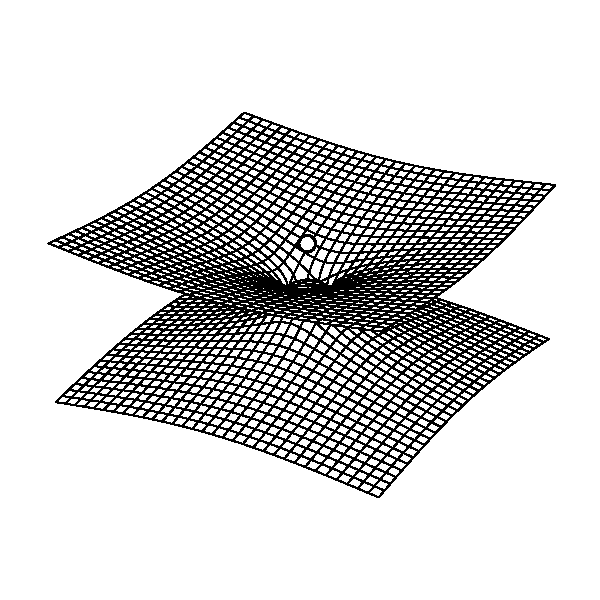
\includegraphics[width=5in]{../covers/P225.pdf}
		\par
		\vspace{1cm}
		{
			\Huge
			\textbf{Lecture Notes on General Relativity}
		}
		\par
		\vspace{0.5cm}
		{
			\Large
			\textsc{Physics 225}\\

			\vspace{0.5in}

			\textsc{Vercil Juan}\\[4pt]
		}
		{
			\large
			\textbf{IV - BS Physics}
		}
		\vfill
		{
			\large
			1st Semester, AY 2026-2027
		}
		
	\end{center}
    
\end{titlepage}
 
	\addcontentsline{toc}{section}{Front Matter}
	\newpage
	\pagenumbering{roman}
	\vspace*{1in}
{\LARGE
	\[
		\Gamma^\rho_{\mu\nu} = \frac{1}{2}g^{\rho\sigma}\qty(\partial_\mu g_{\sigma\nu} + \partial_\nu g_{\sigma\mu} - \partial_\sigma g_{\mu\nu}) \\[20pt]
	\]
	\[
		\dv[2]{x^\sigma}{\lambda} + \Gamma_{\mu\nu}^\sigma \dv{x^\mu}{\lambda} \dv{x^\nu}{\lambda} = 0\\[20pt]
	\]
	\[
		R_{\mu\nu} - \frac{1}{2}Rg_{\mu\nu} = \frac{8\pi G}{c^4}T_{\mu\nu}  
	\]
}

\vfill
{\large
\setlength{\leftmargin}{3cm}
\setlength{\rightmargin}{3cm}
\begin{quote}
	\textit{``Rationem vero harum Gravitatis proprietatum ex Phenomenis nondum potui deducere, et Hypotheses non fingo.''}

	\hfill -- \textsc{I. Newton}
\end{quote}
}

	\newpage
	\begin{center}
	{
		\Large
		\textbf{Physics 225 - General Relativity 1\\[10pt] Course Information}
	}    
\end{center}
\addcontentsline{toc}{subsection}{Course Information}

\subsubsubsection*{Course Description}
	\paragraph{Description: } 
	Manifolds, modern differential geometry and tensor analysis; basic principles of general relativity;
	Einstein field equations and their mathematical properties; exact solutions; linearized theory; variational
	principles and conservation laws; equations of motion; gravitational waves; experimental tests.

\subsubsubsection*{Instructor Details}
	\begin{itemize}[]
		\item[] \textbf{Instructor: } Dr. Michael Francis Ian Vega
		\item[] \textbf{Email: } {\texttt{\url{ivega.upd.edu.ph}}}
		\item[] \textbf{Lecture Hours: } R109, WF, 10:00 - 11:30 AM
		% \item[] \textbf{Classroom Number: } R109
	\end{itemize}

\subsubsubsection*{Course Requirements}
	\paragraph{Problem Sets} 

	Problem sets will be assigned throughout the semester, ideally one per week. These will be
	submitted electronically using a Google Form that I will be sending out close to the deadline. From each
	problem set a random selection of items will be graded. It is your responsibility to ensure that your work
	is neat and legible. If we cannot understand your work then you will not get any credit. These problem
	sets will make up the 30\% of your final grade.

	\paragraph{Written Exam} 
	There will be two written exams in the course. Each exam will constitute 30\% of the final grade.
	These are in-class, open-notes exams. You will have to designate one notebook as your 225
	notebook at the start of the semester. Only this notebook may be used to help you during the exams.

	\paragraph{Oral Exam} This will be scheduled during or shortly after Finals Week. This will make up the remaining 10\%
	of your final grade.



	\newpage
	\section*{Main References}
\addcontentsline{toc}{subsection}{Main References}

We shall not have a main textbook for the class. I used \textit{Schutz}, supplemented by the first edition of \textit{d’Inverno},
when I first started learning GR. I think they are both very good texts. However, I have my own way of
presenting GR that will not always follow the structure or presentation of any single book. My approach is
closest in style to the treatments of \textit{Liang+Zhou} and \textit{Wald}.

There are numerous sources you can refer to. I highly recommend that you look at different texts to help
understand my lectures better. Here are some good books I’ve used on numerous occasions. - \textsc{I. Vega}


\subsubsubsection*{Course Syllabus}
The Syllabus for the course can be found here:
\begin{itemize}
    \item[
        \href{run:C:/Users/verci/Documents/code/Class Notes - V/Physics 225/syllabus/syllabus_ps225_2025.pdf
		}{$\blacksquare$}
    ] 
	\textsc{\href{https://mail.google.com/mail/u/1/inbox
	}{Course Syllabus}}
\end{itemize}

\subsubsubsection*{For General Relativity}

\begin{itemize}[]

	\item[
		\href{run:C:/Users/verci/Documents/Reference Books/Physics/Introducing Einsteins Relativity A Deeper Understanding (Second edition) [d'Inverno, Vickers].pdf
	}{$\blacksquare$}
	]
	R d’Inverno, J Vickers,
	\textbf{\href{https://article.sk/book/Xgvb0ynOge/introducing-einsteins-relativity-a-deeper-understanding-second-edition.html
	}{
		Introducing Einstein’s Relativity: A Deeper Understanding%
	}}, 2022

	\item[
		\href{run:C:/Users/verci/Documents/Reference Books/Physics/Differential Geometry and General Relativity [Liang, Zhou].pdf
		}{$\blacksquare$}
	]
	C Liang and B Zhou,
	\textbf{\href{https://article.sk/book/92rXveVKgv/differential-geometry-and-general-relativity-volume-1.html
	}{
		Differential Geometry and General Relativity%
	}}, 2023

	\item[
		\href{run:C:/Users/verci/Documents/Reference Books/Physics/General Relativity [Wald].pdf
		}{$\blacksquare$}
	]
	R Wald,
	\textbf{\href{https://article.sk/book/9gkDMQrXjm/general-relativity.html
	}{
		General Relativity%
	}}, 1984

	\item[
		$\blacksquare$
	]
	V Ferrari, L Gualtieri, P Pani,
	% \textbf{\href{
	% }{
	% }}
	General Relativity and its Applications%
	, 2021

	\item[
		$\blacksquare$
	]
	T Padmanabhan,
	% \textbf{\href{
	% }{
	% }}
	Gravitation: Foundations and Frontiers%
	, 2010

	\item[
		$\blacksquare$
	]
	A Zee,
	Einstein Gravity in a Nutshell,
	2013

	\item[
		\href{run:C:/Users/verci/Documents/Reference Books/Physics/Spacetime and Geometry [Carrol].pdf
		}{$\blacksquare$}
	]
	S Carrol,
	\textbf{
		\href{https://article.sk/book/Yv2wkYWZ2p/spacetime-and-geometry-an-introduction-to-general-relativity.html
	}{
		Spacetime and Geometry: An Introduction to General Relativity%
	}}, 2003

	\item[
		$\blacksquare$
	]
	Choquet-Bruhat,
	Introduction to General Relativity, Black Holes, and Cosmology,
	2015

	\item[
		$\blacksquare$
	]
	J Hartle,
	\textbf{
		\href{https://article.sk/book/KV2VXKdegp/gravity-an-introduction-to-einsteins-general-relativity.html
		}{
			Gravity: An Introduction to Einstein’s General Relativity%
		}}, 2003. (undergrad)

	\item[
		\href{run:C:/Users/verci/Documents/Reference Books/Physics/A First Course in General Relativity Second Edition [Schutz].pdf
		}{$\blacksquare$}
	]
	B Schutz,
	\textbf{\href{https://article.sk/book/KN26VnNp20/a-first-course-in-general-relativity-second-edition.html
	}{
		A First Course in General Relativity 2nd Ed.%
	}}, 2009. (undergrad)

	\item[
		$\blacksquare$
	]
	MP Hobson, GP Efstathiou, and AN Lasenby,
	General Relativity: An Introduction for Physicists,
	2006. (strong for cosmology)

	\item[
		\href{run:C:/Users/verci/Documents/Reference Books/Physics/Lecture Notes on General Relativity [Hollands, Sanders].pdf
		}{$\blacksquare$}
	]
	S Hollands, K Sanders,
	\textbf{\href{https://www.freebookcentre.net/physics-books-download/Lecture-Notes-on-General-Relativity-by-S.-Hollands-and-Ko-Sanders.html
	}{
		Lecture Notes on General Relativity%
	}}, 2015

	\item[
		\href{run:C:/Users/verci/Documents/Reference Books/Physics/Gravitation and Cosmology [Weinberg].pdf
		}{$\blacksquare$}
	]
	S Weinberg,
	\textbf{
		\href{https://article.sk/book/1ojNn5RzjP/gravitation-and-cosmology-principles-and-applications-of-the-general-theory-of-relativity.html
	}{
		Gravitation and Cosmology%
	}}, 1972

	\item[
		\href{run:C:/Users/verci/Documents/Reference Books/Physics/Relativity - The Special and General Theory [Einstein].pdf
		}{$\blacksquare$}
	]
	A Einstein,
	\textbf{
		\href{https://www.gutenberg.org/files/36114/36114-pdf.pdf
	}{
		Relativity: The Special and General Theory%
	}}, 1920
\end{itemize}


\subsubsubsection*{For Differential Geometry}

\begin{itemize}[]

	\item[
		\href{run:C:/Users/verci/Documents/Reference Books/Physics/Semi-Riemannian Geometry [O'Neill].pdf
		}{$\blacksquare$}
	]
	B O’Neill,
	\textbf{\href{https://article.sk/book/wxWbnq3A2e/semiriemannian-geometry.html
	}{
		Semi-Riemannian Geometry%
	}}, 1983

	\item[
		\href{run:C:/Users/verci/Documents/Reference Books/Physics/Differential Geometry of Manifolds 2nd Ed. [Lovett].pdf
		}{$\blacksquare$}
	]
	S Lovett,
	\textbf{\href{https://article.sk/book/92rldR3Kgv/differential-geometry-of-manifolds-second-edition.html
	}{
		Differential Geometry of Manifolds 2nd Ed%
	}}, 2020

	\item[
		% \href{run:C:/Users/verci/Documents/Reference Books/Physics/Differential Geometry of Manifolds 2nd Ed. [Lovett].pdf
		% }{$\blacksquare$}
		$\blacksquare$
	]
	G Rudolph, M Schmidt,
	\textbf{\href{https://article.sk/book/M6xqNmzPgW/differential-geometry-and-mathematical-physics-part-i-manifolds-lie-groups-and-hamiltonian-system.html
	}{
		Differential Geometry and Mathematical Physics: Part I%
	}}, 2013

	\item[
		\href{run:C:/Users/verci/Documents/Reference Books/Physics/Introduction to Differential Geometry [Robbin, Salamon].pdf
		}{$\blacksquare$}
	]
	J Robbin, D Salamon,
	\textbf{\href{https://webapps.math.uci.edu/~brusso/diffgeom311pp.pdf?utm_source=chatgpt.com
	}{
		Introduction to Differential Geometry%
	}}, 2024
\end{itemize}


\begin{note}
	The hyperlinks in this lecture notes act as follows: The {\color{blue} $\blacksquare$} 
	hyperlink, when pressed, opens the relevant \texttt{pdf} in my (the Author's) local machine. This only
	works for my personal computer. The hyperlink on the {\color{blue}\textbf{name of the book}} links to a source
	of the book on the internet. Press that hyperlink to access that book.
\end{note}

	\newpage
	\section*{Reminders}
\addcontentsline{toc}{subsection}{Reminders}

\subsubsubsection*{Exam Dates}
\begin{itemize}
	\item[$\square$] Long Exam 1 : \textbf{\color{red} October 12, 2026,\quad 9-12 AM} 
	\item[$\square$] Long Exam 2 : \textbf{\color{red} December 7, 2026,\quad 9-12 AM} 
	\item[$\square$] Oral Exam\ \ : \textbf{\color{red} Finals week (TBA)}
\end{itemize}

\subsubsubsection*{Problem Set Dates}
\begin{itemize}
	\item[$\square$] September 29, 2026.
	\item[$\square$]
	\item[$\square$]
	\item[$\square$]
	\item[$\square$]
\end{itemize}


	\newpage
	
\section*{Preface}
\addcontentsline{toc}{section}{Preface}
\vspace{0.5cm}
\hspace{2em}Relativity. When I was a child, I remembered wondering why things go down the way they do.
My folks and those who are older just answer to me: That's simply the way things are. Later on,
when I was older, I picked up this old book called \textit{Science in Daily Life} where I learned
much about science and chemistry and all those good shit. That book was one of my prized posessions,
I still have it today, in fact. When I was a little older, right around fourth grade, my neighbor
was throwing out books she no longer used, and part of that mixture were books on chemistry and 
books on Physics. 

It was there where I learned about Newton and his apple. It was there where I learned about Einstein and
binding energies and logic gates, of nuclear physics and atom bombs; where I learned that gravity is a force that drew upon it other 
masses by the product of their quantities the inverse of the square of their distances. That made me interested in orbital mechanics,
astronomy, the Apollo program. That book was one of the reasons why I am where I am today. I say 
all this, because we all have an origin story of some sort. Some story we call ours, that tells 
our own humble beginnings. This was a story of how I fell in love in Physics, and why I chose it
to be my career once I reached adulthood. That's why I decided to be a Physicist.

Newton had origin stories. Einstein had an origin story. We must treasure where we came from, and 
what it took for us to get there, is all I'm trying to say. Anyways, I first leard about general 
relativity all those years ago, but thought it was very difficult and a hassle to understand. Understanding
special relativity and its implications were much easier, but boy, GR is a whole 'nother level. 
But fascinating! Differential geometry, manifolds, paradoxes, black holes, all so fascinating and interesting
for me, part of the reason why I fell in love with the damn philosophy of reason. But also, scary,
all those numbers and derivatives and the like, all so intimidating, that I thought back then I 
would never even learn it. And so, I 
find it funny, now, as an adult, that I took it as my undergraduate specialty of choice, joining
a laboratory that specialized in gravity, taking my thesis on gravity. The amount of difficult mathematics
one had to master to reach this point is insane, but, much like a mountain, the difficulty is part
of the journey, and to reach the top is sweeter than the pleasures we get to enjoy in our daily life.

And so, here I am today, taking a graduate course in my undergraduate degree, about the subject that
fascinated me as a child, but I found too difficult to climb and learn. Now, I know enough to say
that what I know is a drop in an endless ocean, and relativity, the jewel of modern physics, in 
both beauty and elegance, is the pearl at the bottom of it.
It makes me glad that it is what I chose to dedicate my academic life to, and I find within me
the desire to add to the sum of human knowledge, to leave a legacy behind and be remembered
in such way. It is only recently that I learned
to appreciate physics for what it is, a beautiful description of reality. In my early college years, the
stress of it all consumed me, and now I am about to graduate, I look back think of all those things 
I learned, and it impresses me that I could learn so much.

Anyways, these lecture notes are precisely that, transcriptions of lectures on the course of General Relativity,
by one of the leading physicists in the country, Dr. Vega, whom I personally idolized since I
learned about him when I was in highschool, being a homegrown gravitational physicist and all that,
and now I'm studying under him, ain't that something.
The content is precisely what he talks about in the lecture. Although not exactly verbatim, I tried 
my best to record all the words being said and tried to capture the topic being discussed at the moment,
doing my best to convey the idea and meaning of the lecture. So that, in the future, I may look upon it when I forget something or simply
as I please, and others, peers, students, friends, which I may give these lecture
notes to, may understand it in a manner that I understand it today. I wish the future may be kind to us,
and when we look back, to our stories and origins, may we smile and reminisce in mild happiness,
and be proud of what we have become.

\begin{flushright}
	\textbf{Vercil Juan}\\
	\textrm{V - BS Physics}\\
	\textsc{University of the Philippines Diliman}
\end{flushright}
\vfill
\begin{center}
	{
		\large
		\textsc{Physica Vincit Omnia}
	}
\end{center}

	\newpage
	{
	\hypersetup{linkcolor=black}
	\addcontentsline{toc}{subsection}{Contents}
	\tableofcontents
	\newpage
	\addcontentsline{toc}{subsection}{List of Figures}
	\listoffigures
	\newpage
	\addcontentsline{toc}{subsection}{List of Definitions}
	\listofdefinitions
	\newpage
	\addcontentsline{toc}{subsection}{List of Theorems}
	\listoftheorems
}

	\newpage
	\pagenumbering{arabic}
	\chaptersec{Review of Newtonian Physics}
		%date --- 12 - 08 -26

\subsection{Introduction}

	\begin{quote}
		\hspace{1em}``That gravity should be innate, inherent, and essential 
		to matter, so that one body may act upon another at a distance through
		a vacuum, without the mediation of anything else... is to me so great
		an absurdity that I believe no man who has, in philosophical matters,
		any competent faculty of thinking can ever fall into it."
		\hfill --  \textsc{Newton}
	\end{quote}
	We begin this course with the assumption that you have no idea what General Relativity is.
	How do we quantify what is gravity? What even is gravity? We begin with the classical equations of motion.

	The classical equations of motion, first described by Galileo and formalized by Isaac Newton, 
	have long served as the default model for describing the behavior of classical objects under 
	the influence, or lack thereof, of external forces, and remain a fundamental part of physics
	education due to their success in describing matter within the scope of ordinary human observation.
	However, in the dawn of the 20th century, contradictions between these classical descriptions
	and experimental observations began to surface, making it apparent that a new description of
	reality was needed to reconcile theory with these results.

	To motivate ourselves, we describe three concepts introduced over the history of classical mechanics and explain how 
	it leads to certain contradictions or problems that motivated the realization and invention of general relativity
	\newpage
	\subsubsection{Newton's Law of Gravitation}

		Newton's Laws as he prescribed them is expressed as follows:
		\begin{equation}
			m_N\dv[2]{\vb{x}_N}{t} 
			= 
			G \sum_M 
			\frac{
				m_N m_M (\vb{x}_M - \vb{x}_N)
			}{
				\norm{\vb{x}_M - \vb{x}_N}^3
			} 
		\end{equation}
		More often, it is shortened as:
		\begin{definition}{Newton's Law of Gravity}
			\begin{equation}
				\vb{F} = -\frac{GMm}{r^2}\vb{\hat{r}} 
			\end{equation}
		\end{definition}

		This is the familiar form of Newtonian gravity, and is perhaps one of the most recognizable equations in physics.
		This is what every high schooler knows and what every mentor presents, and is trivial to derive via experimentation.

		We can separate the mass $m$ experiencing the force from the mass $M$ producing it, and write

		\begin{equation}
			\vb{F} = m_g \qty(-\frac{GM}{r^2}\hat{\vb{r}})
		\end{equation}

		We can henceforth call $m_g$ as the \textit{gravitational mass} and the quantity $-\dfrac{GM}{r^2}\hat{\vb{r}}$ as the \textit{gravitational field}

		We can express it more generally by recognizing the force field is simply the negative gradient of a potential field.
		\begin{equation}
			\vb{F} = m_g\qty(-\grad\Phi)
			\label{eq: F = mg x -gradphi}
		\end{equation}
		where $\displaystyle \Phi = -\frac{GM}{r} $ is the gravitational potential produced by the source mass.

		Thus, we can henceforth call $m_g$ as the \textit{gravitational charge}. It follows from the fact that
		\begin{equation}
			\text{charge}\times \text{field gradient} = force
		\end{equation}
		This formulation is universal across all of physics.

		Analogous to electromagnetism, where 
		\begin{equation}
			\vb{F} = \frac{1}{4\pi\varepsilon_0} \frac{q_1 q_2}{r^2}\hat{\vb{r}} 
		\end{equation} 
		Like the electric charge $q$, the gravitational charge $m_g$ determines the strength of the interaction of the forces.

		An important property that Newtonian gravitation has is that it has superposition. i.e., fields add together linearly.
		This is therefore also true of the gravitational potential.

		For a system of point masses, the total potential field $\Phi(\vb{x})$ at a point $\vb{x}$ is given by the sum of the potentials produced by each individual mass:

		\begin{align*}
			\Phi(\vb{x}) &= \sum_i \Phi_i \\
						 &= -G\sum_i \frac{M_i}{\abs{\vb{x}-\vb{r}_i}} 
		\end{align*}

		We can extend this description from a discrete collection of point masses to a continuous mass distribution.
		Let the mass contained in an infinitesimal volume $\dd[3]{\vb{r}}$ be

		\begin{equation}
			dm_i = \rho(t,\vb{r}) \dd[3]{\vb{r}}
		\end{equation}
		Then we arrive with the continuum version of the gravitational potential field generated by a mass distribution.
		\begin{equation}
			\Phi(\vb{x}) 
			= - G \int \frac{
			\rho(t,\vb{r})}{\abs{\vb{x}-\vb{r}}} 
			\dd[3]{\vb{r}}
		\end{equation}

		Here, $\vb{r}$ denotes the position of each source element of the mass distribution, while $\vb{x}$ denotes the point at which the potential is being evaluated.

		We can now obtain a differential equation for the gravitational potential. Taking the Laplacian of $\Phi$ gives

		\begin{equation}
			\lpc \Phi = -G \int \rho(t,\vb{r})\dd[3]{\vb{r}} \lpc \frac{1}{\abs{\vb{x}-\vb{r}}}
		\end{equation}
		Recall that this operation results to a dirac-delta function
		\begin{equation}
			\lpc \frac{1}{\abs{\vb{x}-\vb{r}}} = - 4\pi\delta(\vb{x}-\vb{r})
		\end{equation}

		which relates the Laplacian of the inverse-distance potential to the Dirac delta function. Substituting this into the previous expression gives

		\begin{equation}
			\lpc \Phi = 4\pi G \int \rho(t,\vb{r})\dd[3]{\vb{r}} \delta(\vb{x}-\vb{r})
		\end{equation}
		Recall the sifting property of the Dirac delta
		\begin{equation}
			\int f(r)\delta(x-r) \dd{r} = f(x)
		\end{equation}
		From this we obtain	
		\begin{equation}
			\lpc \Phi = 4\pi G \rho(t,\vb{x})
		\end{equation}
		Since $\vb{x}$ is an arbitrary point, we may relabel it as 
		\begin{equation}
			\lpc \Phi(t,\vb{r}) = 4\pi G \rho(t,\vb{r})
		\end{equation}
		Thus, we arrived with the fundamental field equation which governs Newtonian Gravity

		\begin{theorem}{Field Equation for Newtonian Gravity}
			\begin{equation}
			   \lpc \Phi = 4\pi G \rho  
			\end{equation}
		\end{theorem}
		The significance of a field equation is that it relates a field to its sources. In this case, the mass density $\rho$ acts as the source of the gravitational potential field $\Phi$. 
		
		Note the following
		\begin{equation}
			\Phi = -G\int \frac{\rho \dd[3]{\vb r}}{\abs{\vb{x}-\vb{r}}} 
			\iff \lpc\Phi = 4\pi G \rho 
		\end{equation}

		The two are notionally equivalent. One is a differential equation and the other is the integral form. One can switch
		to and from them using the Laplacian and Green's functions\footnote{Green's functions are essentially the inverse of a laplacian, $\nabla^{-2}$}.
		It assigns the definition of the field, and fields assign values to every point in space.

		However, this formulation presents a fundamental problem. Since the potential $\Phi$ is determined directly by the mass density $\rho$, any change in the mass distribution produces 
		an immediate change in the gravitational field throughout space. There is no propagation delay or retardation. In other words, Newtonian gravity permits changes in the gravitational
		field to propagate instantaneously, which is incompatible with relativistic causality. This problem is one of the motivations for general relativity. 

		The corresponding requirement in GR is that, in the appropriate weak-field and slow-motion limit, general relativity must reduce to Newtonian gravity.

		Now that we have the potential of the field that the source creates, and thus the force, how do we determine how an object moves in response to that field?
		% \newpage
	\subsubsection{Newton's Equations of Motion}
		The quintessential equation governing the motion of classical bodies was expressed by Newton as
		\begin{equation}
			\vb{F} = m\vb{a}
		\end{equation}
		Everybody and their mother knows this shit.

		This states that if one sums of all the forces acting on an object, 
		it must equal its mass multiplied by its acceleration:
		\begin{equation}
			\sum\vb{F} = m\vb{a}
		\end{equation}
		We can rewrite the equation as
		\begin{equation}
			\vb{a} = \frac{1}{m} \sum \vb{F}
			\label{eq: a = 1/m f}
		\end{equation}

		Notice that the $m$ term acts as a kind of \textit{resistance} term\footnote{Recall Ohm's Law $V = IR$.}, similar to the concept of inertia. This is to be expected, since Newton's first law can essentially be understood as the statement that, in the absence of a net force, an object does not change its state of motion.

		Hence, we name this quantity the \textit{inertial mass}, $m_i$. Inertia denotes the difficulty or resistance of an object to a change in its state of motion.

		We can restate (\ref{eq: a = 1/m f}) with $m$ replaced by $m_i$, to distinguish inertial mass from the gravitational mass introduced previously:
		\begin{equation}
			\vb{a} = \frac{1}{m_i} \vb{{F}}
		\end{equation}

		Recall that we already have the definition of $\vb{F}$ from (\ref{eq: F = mg x -gradphi}). Thus, to calculate the motion of an object under the influence of gravity, we simply calculate its acceleration:
		\begin{equation}
			\vb{a} = \frac{m_g}{m_i}\qty(-\grad\Phi)
		\end{equation}

		Notice that this is similar in form to the equation of motion for a charged particle in an electric field.
		\begin{equation}
			\vb{a} = \frac{q}{m_i}\vb{E}
		\end{equation}
		where $m_i$ is the inertial mass, the measure of an object's resistance to changes in its motion. In both cases, the coupling to the field determines the force, while the inertial mass determines the resulting acceleration.

		However, for calculations involving Newtonian gravity, the ratio of the gravitational charge and inertial mass
		$\displaystyle \frac{m_g}{m_i}$ is assumed to be $1$. Thus, for gravity, the acceleration of a body is expressed as
		\begin{equation}
			\vb{a} = -\grad\Phi.
		\end{equation}
		This assumes that
		\begin{equation}
			m_g = m_i,
		\end{equation}
		This feels unnatural and unexpected, a truly remarkable coincidence in Newtonian theory. Why should it be the case that one force acts differently from other forces in terms of its charge carriers?
		Mass is a fundamental property that affects other forces, there's no immediate evidence why mass is gravity's charge carrier.

		There is no \textit{a priori} reason why the magnitude of gravitational force on a particle should equal the quantity that determines the particle's resistance to an applied force in general. 
		They play fundamentally different roles in the theory. It is 
		analogous to assuming that an object's coupling to some other field must be equal to 
		its inertial mass, like an electron's electromagnetic properties being dependent on mass.

		Nevertheless, for gravity this equality is accepted experimental fact without explanation. 
	

	\subsubsection{Weak Equivalence Principle}
		The assumption that
		\begin{equation}
			m_i=m_g
		\end{equation}
		is called the \textit{weak equivalence principle}.

		It follows that, for objects \underline{only} affected by gravity, the equation of motion is simply
		\begin{equation}
			\vb{a} = -\grad\Phi.
		\end{equation}

		That is, any test mass placed in the same gravitational field experiences the same acceleration, regardless of its mass or composition. The nature of the object itself does not appear in the equation of motion. The field prescribes the acceleration, the test body merely responds to it.

		One could therefore remove the test object $m$ and nothing about the gravitational field would change. In Newtonian mechanics, this is treated as a universal fact: the gravitational field exists independently of the particular body used to probe it.

		However, this raises a deeper question.

		One could argue that the stage for the motion of an object is the field itself. If we remove the object from some local region, the field remains.

		By the same logic, if we remove the field itself, what remains? In Newtonian mechanics, space $\R^3$ remains as the stage on which the field and matter exist.

		The influence of gravity has \underline{nothing} to do with the nature of the test object itself. The gravitational field does not change when the test object is removed, and its motion depends only on the field at its location.

		One might ask: if we remove all mass, would there not be no gravity? The answer is that we must distinguish the sources of the field from the test body. We are considering local interactions. Mass may exist somewhere outside the local region of interest and still generate a gravitational field within it. Given the local potential $\Phi$, we can determine information about its sources, but the test body itself is not one of those sources.

		Thus,
		\begin{equation}
			\vb{a} = -\grad\Phi
		\end{equation}
		is treated as inertial motion in a gravitational field.

		In the stage analogy, one could think of $-\grad\Phi$ as living on the stage of space $\R^3$. The field exists on space and determines how objects move through it. 
		In some fields such as particle physics, that is the case, they treat gravity as a special field  which acts on every particle and every particle responds to in the same way

		However, in GR, $-\grad\Phi$ is no longer treated as a field sitting on top of the stage. The gravitational field \textit{is} the stage. 
		The space time is what the rest of physics takes place in.

		The strong equivalence principle extends this idea: locally, the laws of physics in a freely falling frame are the same as those of an inertial frame in the absence of gravity. In other words, locally, gravity can be transformed away by choosing an appropriate freely falling frame.

		Inertial motion is therefore determined by the structure of spacetime.

		Physics takes place on the stage called spacetime, and GR governs that space time. The spacetime structure remains even after the particular body used to probe it is removed.

		In GR, instead of the gravitational potential field $\Phi$, we have the metric:
		\begin{equation}
			ds^2 = g_{\mu\nu} dx^\mu dx^\nu.
		\end{equation}

		The metric determines the geometry of spacetime and, consequently, the inertial trajectories of objects.

		In particle physics, one generally begins with a fixed flat spacetime $\R^4$ and defines fields upon that background. Gravity can then be treated as a field on this background, rather than as the geometry of spacetime itself. This approach is sound as a field-theoretic formulation and provides a natural route toward quantizing gravity and describing gravitons, but it is ugly and inelegant. Regardless, you can bootstrap yourself from there and arrive on the EFE

		The distinction of perspectives can be summarized as follows:
		\begin{center}
			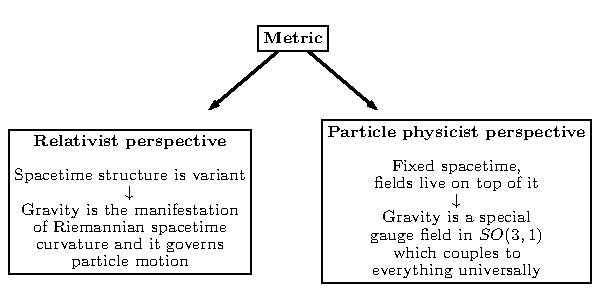
\includegraphics[width=4in,height=2in]{images/metricperspective.pdf}
		\end{center}
		Regardless of the formalism, the different approaches must reproduce the same classical predictions. The geometric formulation of GR ultimately leads to the Einstein field equations.
	\subsubsection{A Theory of Gravity}
		General Relativity, to be a theory of gravity, must explain gravitational phenomena.

		For example, Newtonian gravity became a theory of gravity because it explained the results Kepler had found. Kepler described the motion of the planets and discovered that their orbits were elliptical using data analysis, but he did not have an underlying physical theory explaining \textit{why} they followed these trajectories.

		Newton instead derived the observed behavior from first principles. His laws of motion and universal gravitation explained Kepler's laws and provided a general framework for celestial mechanics, and ended up predicting the whole of kinematics and dynamics.

		As such, GR as a theory of gravity must be able to explain observed gravitational phenomena: relativistic corrections to celestial mechanics, gravitational waves, black holes, gravitational collapse, and, on the largest scales, cosmology.

		Perhaps the grandest application of GR is cosmology. Newtonian gravity is fundamentally a local theory applied within a fixed space and time, while GR allows the spacetime itself to be dynamical. This makes it possible to formulate a theory describing the universe as a whole.

		\paragraph{DISTINCTION:
		} For something to be a theory of gravity, what must it possess?

		\begin{enumerate}
			\item \textbf{Dynamical variables}

			The theory must have variables describing the gravitational field in which objects move.

			\begin{align*}
				\text{Newton:} \qquad &\Phi\\
				\text{GR:} \qquad &g_{\mu\nu}
			\end{align*}

			\item \textbf{A law describing how the field affects objects}

			The theory must describe how its dynamical variables determine the motion of objects.

			For Newtonian gravity:
			\begin{equation}
				\vb{a} = -\grad\Phi.
			\end{equation}

			For GR, freely falling objects follow geodesics:
			\begin{equation}
				\dv[2]{x^\sigma}{\lambda} 
				+
				\Gamma^\sigma_{\mu\nu}
				\dv{x^\mu}{\lambda} 
				\dv{x^\nu}{\lambda} 
				=0,
			\end{equation}
			or, using the four-velocity $u^\mu$,
			\begin{equation}
				u^\mu\grad_\mu u^\nu = 0.
			\end{equation}

			\item \textbf{A law describing how objects produce the dynamical variable}

			Finally, the theory must tell us how matter produces the gravitational field.

			For Newtonian gravity:
			\begin{equation}
				\lpc\Phi = 4\pi G\rho.
			\end{equation}

			For GR:
			\begin{equation}
				R_{\mu\nu}
				-\frac{1}{2}g_{\mu\nu}R
				=
				8\pi G T_{\mu\nu}.
			\end{equation}
			Since the two formalisms attempt to explain the same phenomenon, we demand
			that the GR formulation reduces to the Newtonian formulation in weak fields.
		\end{enumerate}
		\par
		\begin{remark}
			Notice that $\lpc \Phi = 4\pi G \rho$ and $
					R_{\mu\nu}
					-\frac{1}{2}g_{\mu\nu}R
					=
					8\pi G T_{\mu\nu}
					$ 
			are inherently similar. They basically describe the same thing, but in different fields of geometry.
			Note the following:
			\begin{align*} 
				\underbrace{\lpc\Phi}_{\text{some combination of }\partial^2} &= \underbrace{4\pi G\rho}_{\text{constant multiplied to matter distribution}}
				\\
				\underbrace{R_{\mu\nu}
				-\frac{1}{2}g_{\mu\nu}R}
				_{\text{some combination of }\partial^2}
																	   &=
				\underbrace{8\pi G T_{\mu\nu}}
				_{\text{constant multiplied by matter distribution}}
			\end{align*}
		\end{remark}
		These three ingredients are the basic structure of a theory of gravity: a dynamical variable, a law governing how it affects matter, and a field equation governing how matter produces it.

		GR is inherently nonlinear. Going from the field to the motion of objects is already more complicated than in Newtonian gravity, but the field equation itself is also nonlinear: the metric determines the curvature, while the curvature determines the metric.

		Solving the Einstein field equations for realistic systems is therefore often extremely difficult. In many cases, exact solutions cannot be obtained, and the equations must be solved numerically. Careers have been made doing this. This is the domain of \textit{numerical relativity}.

		In the next chapters, we will explore how gravity can be explained by general relativity.

		\newpage
		% =======================================
% MEETING 2
% ---------------------------------------
% DATE   - AUGUST 14, 2026
% FORMAT - FACE TO FACE
% =======================================
% TOPIC  - EQUIVALENCE PRINCIPLE
% =======================================

\subsection{Einstein's Equivalence Principle}

	\subsubsection{Inertial Frames}

		The Weinberg definition is that, at every point in spacetime, i.e. at every $(t,x,y,z)$ 
		in a gravitational field, it is possible to choose a locally inertial frame, i.e. a freely 
		falling coordinate system, such that the ``laws of nature'' take the same form as they do in 
		an unaccelerated Cartesian coordinate system in the absence of gravity.

		In other words, fields that are accelerating are locally indistinguishable from gravity. 
		This is the basic idea behind the equivalence principle.

		Gravity can therefore be regarded as a fictitious force, because it can be removed by a 
		coordinate transformation. It is there only because we are using the wrong coordinate system.

		The equivalence principle states that it is always possible to remove gravity locally. 
		Therefore, gravity is a fictitious force'' that can be ``removed'' when describing the 
		local field in an experiment.

		The important difference between gravity and other fictitious forces is that gravity can 
		only be removed locally, while other fictitious forces can be removed globally. 
		The reason is that a gravitational field has spatial variation. Even after transforming 
		away the gravitational acceleration at one point, neighboring points may experience 
		slightly different accelerations.

		We say that, regardless of the mass of the object, it does not take part in determining 
		its own gravitational acceleration. The gravitational acceleration is universal.

		The measurement of differences between these gravitational fields is called \textit{tidal} measurement, 
		or simply the measurement of tides. These tidal effects cannot be transformed away over an extended 
		region.

	\subsubsection{Universality of Free Fall}

		The usual way this is expressed is to imagine a person in a closed box with no reference to the outside world. To gain 
		information about his environment, he begins conducting a free-fall experiment. Suppose they perform some experiment in 
		which they can measure the acceleration of objects.

		For an object $o_1$, they measure

		\begin{equation}
			\vb{a}_1 = \frac{m_{1g}}{m_{1i}} \vb{g}
		\end{equation}

		and for a second object $o_2$, they can measure

		\begin{equation}
			\vb{a}_2 = \frac{m_{2g}}{m_{2i}} \vb{g}.
		\end{equation}

		The universality of free fall is the statement that

		\begin{equation}
			\vb{a}_1 = \vb{a}_2
		\end{equation}

		under the same circumstances, regardless of the nature or mass of the objects. This is called the \textit{universality of free fall}.
		
		Suppose that the box is accelerating upward with acceleration $g\vu{z}$.
		\begin{equation}
			\vb{a}_\text{box} = g\vu{z}
		\end{equation}

		The observer releases the ball. From his perspective, the ball appears to accelerate downwards.
		\begin{equation}
			\vb{a}_\text{ball} = -g\vu{z}
		\end{equation}
		Therefore, it is reasonable to conclude that ``there is a gravitational field pulling the force downward".

		But there isn't. The ball is actually just continuing along its inertial trajectory while the box accelerates upward.

		Now compare this with another box which is stationary, with another observer sitting on the surface of Earth.

		The observer releases the same ball, and it falls downward with approximately

		\begin{equation}
			\vb{a}_\text{ball} = -g\vu{z}
		\end{equation}
		Inside the box, the experiment looks the same. So locally, motion due to acceleration is indistiguishable from motion
		incduced by a gravitational field. There is no experiment that can be performed by the two observers that can differentiate
		one from another. This is the strong equivalence principle.

		In Newtonian language, this corresponds to the equality of gravitational and inertial mass. The important point for the equivalence principle is that all sufficiently small freely falling objects respond to the gravitational field in the same way.

		Now, imagine the observer is in a box or elevator that is freely falling towards Earth.
		The box and everything inside it are accelerating downward together.
		Suppose the observer release a ball inside the box.
		The ball is falling toward Earth, but so is the box. Since both have essentially the same gravitational acceleration,
		\begin{equation}
			\vb{a}_\text{ball}\approx \vb{a}_\text{box}
		\end{equation}
		their relative acceleration is approximately zero:
		\begin{equation}
			\vb{a}_\text{relative} = \vb{a}_\text{ball} - \vb{a}_\text{box} \approx 0
		\end{equation}
		so the ball appears to float. The observer could throw it, and it would move approximately in a straight line at constant velocity relative to the observer.

		The observer would therefore reasonably conclude ``There is no gravity here. I'm in an inertial frame."

		But the observer actually is in Earth's gravitational field. In actual inertial motion, far from any gravitating bodies, the same observations will take place.
		Therefore, a falling observer is indistinguishable from an inertial observer. That is the weak equivalence principle.


		In a simple example, we can write the gravitational field as a non-inertial frame:

		\begin{equation}
			\ddot{y} = - g
		\end{equation}

		We can remove gravity, however, via certain transformations. Let

		\begin{equation}
			z = y - \frac{1}{2}gt^2
		\end{equation}

		This results in

		\begin{equation}
			\ddot{z} = 0.
		\end{equation}

		This is an inertial coordinate system, since there is no perceived acceleration. The point is that gravity can be removed locally by choosing an appropriate freely falling coordinate system.

		The person in the box cannot tell whether they are accelerating upward with constant acceleration $g$, or whether they are freely falling under the influence of gravity. In a sufficiently small region, the two situations are experimentally indistinguishable.

		Gravity is therefore, locally, simply the manifestation of being in the wrong frame.

		\textit{Inertial} means the absence of gravitational acceleration in the local frame. More precisely, an inertial frame is one in which freely falling objects move without coordinate acceleration.

		\paragraph{Weak, Strong, and Einstein Equivalence Principles}

			We have the weak equivalence principle, where the ``laws of nature'' are understood primarily as the laws of mechanics and the universality of free fall.
			For the strong equivalence principle, one extends the statement to gravitationally self-interacting or strongly gravitating systems, so that the equivalence applies more broadly than to test particles alone.

			The Einstein equivalence principle goes further: ``laws of nature'' genuinely means all laws of nature. It is one of the conceptual foundations of general relativity.
			\begin{theorem}{The Principle of Relativity}
				\label{thm:principle_of_relativity}
			    The laws of nature take the same form in all inertial observers.
			\end{theorem}
			
			In any theory of gravity, one can attempt to remove $g$ locally by an appropriate choice of coordinates. What makes general relativity special is the geometric interpretation of what remains after the local gravitational acceleration has been removed.

			It means that gravity is genuinely fictitious locally if no experiment confined to that sufficiently small region can tell that we are in a gravitational field. If one can remove gravity, then what remains should be the stage itself: the underlying spacetime structure and its geometry.

			In summary, over a sufficiently small region of space and time, a fictitious gravitational field produced by acceleration is indistinguishable from a gravitational field produced by mass (strong equivalence principle).
			Likewise, within a sufficiently small region of space, a freely falling observer cannot distinguish between free fall in a gravitational field and inertial motion in the absence of gravity (weak equivalence principle). 
			Therefore, a freely falling observer is locally an inertial observer.
\subsection{History of Relativity}

	The notion of inertiality plays a major role in relativity. Let us first explain relativity in its historical context.

	We begin with special relativity and Newtonian gravity. The combination of these ideas eventually leads us toward general relativity, where gravity is incorporated into the structure of spacetime itself.

	\subsubsection{Relativity before Einstein}

		What is relativity? It is an old notion that existed even by the time of Newton. The essential idea is that there should exist observers for which the laws of nature take the same form. Regardless of where the observer is or how they move within the appropriate class of frames, the laws of nature should be invariant.

		This is the equivalence of \textit{inertial observers}: the laws of nature take the same form for all inertial observers.

		Aristotle did not have this notion. He believed that there was a special place toward which objects naturally moved: the center of the universe, identified in practice with the center of the Earth. One could therefore imagine that this special region defined the natural frame in which the laws of nature took their proper form.

		It made sense within that picture to express physics relative to the center of the Earth, since all other frames could be considered as moving relative to this preferred location. For example, one could imagine waves in a pond as being fixed relative to the pond itself, with the pond providing a preferred rest frame.


		Galileo rejected this notion by positing that there is not a single preferred inertial state. Instead, there is a class of observers for whom the laws of mechanics are equally valid. These observers move uniformly relative to one another.

		This is called \textit{Galilean relativity}. There is a class of observers which all move relative to each other with uniform velocities.

		The transformation between two such frames can be written as
		\begin{align}
			t' &= t\\
			\vb{x}' &= \vb{x} - \vb{v}t
		\end{align}

		This relation explains how one can switch to the frame of reference of a second observer moving at velocity $\vb{v}$ relative to the first.

		In that case, one has the following invariance of Newtonian mechanics:

		\begin{equation}
			\vb{F} = m\vb{a} \implies \vb{F}' = m\vb{a}'.
		\end{equation}

		Newtonian theory therefore satisfies Galilean relativity: it is invariant under Galilean transformations.

		From the development of Newtonian mechanics onward, classical mechanics became the fundamental framework of physics.
		From 1687 onwards, the only fundamental laws of physics is Newtonian physics.

	\subsubsection{Maxwell's Results}

		For roughly three centuries, Newtonian mechanics was the jewel of physics. Then electromagnetism broke this picture.

		In 1862, Maxwell showed that Maxwell's equations are not Galilean invariant. They therefore do not satisfy Galilean relativity in the same way that Newton's equations do. This challenged centuries of orthodoxy.

		The response of academia was initially to deny that Maxwell's equations were fundamental in the same sense as Newtonian mechanics. One possibility was that Maxwell's equations were only correct in the rest frame of some physical medium, and that medium was called the \textit{aether}.

		The aether was imagined as an invented medium through which electromagnetic waves propagated. This was reasonable at the time, since
		all known waves needed a medium to travel from one place to another, think of sound or earthqakes or water waves.
		In this picture, Maxwell's equations described electromagnetic waves in the same broad conceptual sense that waves 
		in a pond are described relative to the pond.

		Light, therefore, would then only move at speed $c$ only in the rest frame of the aether.

		This led naturally to attempts to detect the Earth's motion through the aether, such as the Michelson-Morley experiment. However, the results of the experiment was null; the expected difference in the measured speed of light was not observed, and the result indicated that $c$ was the same in all different experimental directions.

		People fought against this result, as they should have. The natural response to an experimental discrepancy is to try to preserve a successful theory if possible and search for a physical explanation for the new result.

	\paragraph{Ad Hoc Solutions to the Aether Problem.}

		One proposed solution was Lorentz contraction. Objects would contract in the direction of motion through the aether, although there was initially no satisfactory physical explanation for why they should do so. It was essentially an ad hoc solution introduced to maintain consistency with the null result.

		Another proposed idea was \textit{ether dragging}. Imagine that the ether is not a fixed frame, but behaves something like molasses or syrup, so that the Earth in motion drags the ether around it. The Earth would then remain locally at rest with respect to the ether, and there would consequently be no observed change in $c$.

		The debates went on for decades. People had built careers around various versions of these theories, and many ad hoc solutions were introduced to preserve the compatibility of Maxwell's theory with Galilean relativity.

		There were dozens of theories introduced in the hope of making Maxwell's equations consistent with the Galilean framework.

	\subsubsection{Einstein's Contribution}

		Einstein came in 1905 with his \textit{annus mirabilis} papers.

		The three major papers associated with this period gave rise to major developments in quantum theory, statistical mechanics, and special relativity. Einstein developed these ideas all before turning 24.

		Everyone had been focused on finding a way to mesh Galilean relativity with Maxwell's equations. The common strategy was to deny the fundamentality of Maxwell's equations by claiming that they only worked in the preferred frame of the aether.

		Einstein instead reversed the argument.

		Einstein posited that Maxwell's equations are fundamental, while Newtonian mechanics is not fundamental. Newtonian mechanics was a theory that had been successful for three centuries, but its enormous historical success did not make it fundamentally immune to revision.

		His solution is:

		\begin{itemize}
			\item adopt $c$ as universal;
			\item accept Maxwell's equations as fundamental.
		\end{itemize}

		As such, the equations governing Galilean relativity must be dropped so that $c$ remains constant. By consequence, one also has to give up or modify Newtonian mechanics and stop treating it as fundamentally exact.

		One has to divorce oneself from the notion that Newtonian mechanics is fundamental.

		The notion of universal observers is still true: there is a class of observers for whom the laws of motion retain the same form. However, to reconcile this with the invariance of $c$, one must change the transformation law between observers.

		This leads to the unification of space and time and to the Lorentz transformations.

	\paragraph{Lorentz Transformations and Covariance}

		Maxwell's theory is relativistic, meaning that is relativistically covariant: under the appropriate relativistic transformations, its mathematical form does not change.
		This covariance is not apparent in the separate electric and magnetic fields, which transform into one another between inertial frames. Relativity instead unifies them as aspects of a single electromagnetic field.

		The task is therefore to find the correct transformation laws that keep Maxwell's equations invariant.
		These transformations will replace the Galilean transformation laws and reveal the kinematic structure required by electromagnetism.

		It is then found that the Poincar\'e-Lorentz transformations, initially formulated to explain the null result of Michelson-Morley and to save the aether hypothesis, provide the appropriate transformations:
		\begin{theorem}{Lorentz Transformations}
			Transformations of coordinates that allow $c$ to be invariant across all inertial observers.
			\begin{align}
				ct' &= \gamma(ct-\beta x) \\
				x'  &= \gamma(x - \beta ct) \\
				\gamma &= \frac{1}{\sqrt{1-\beta^2}} \\
				\beta &= \frac{v}{c}.
			\end{align}
		\end{theorem}

		The project, according to Einstein, is to rewrite all of physics so that it is in ``relativistically covariant'' form: the equations 
		should be invariant in form from one inertial observer to another\footnote{This isn't too difficult back in 1905, since the only fundamental theories of physics at the time were Newton's and Maxwells.}.

		The form of these transformations is the Lorentz transformations. (See \S\ref{subsubsec:lorentz-transformations})
		\begin{equation}
			x'^{\mu} = \tensor{\Lambda}{^\mu_\nu} x^\nu.
		\end{equation}
		where
		\begin{equation}
			x^\mu = (ct, x^1, x^2, x^3)
		\end{equation}
		and
		\begin{equation}
			\tensor{\Lambda}{^\mu_\nu} =
			\bmqty{
				\gamma & -\gamma \beta & 0 & 0\\
				-\gamma \beta & \gamma & 0 & 0 \\
				0 & 0 & 1 & 0 \\
				0 & 0 & 0 & 1
			}
		\end{equation}

		Now, the force equation becomes
		\begin{equation}
			\dv{\vb{p}}{t} = \vb{F}\implies \dv{p^\mu}{\tau} = F^\mu.
		\end{equation}
		The second equation (the four momentum and the four force) reduces to the first equation (the Newtonian vector form),  in the appropriate nonrelativistic, low-velocity limit.

	\paragraph{How About Gravity?}

		Gravity is simply

		\begin{equation}
			\lpc\Phi = 4\pi G \rho.
		\end{equation}

		This is not relativistically covariant, since it is written as a theory involving only space and does not incorporate space and time into a unified relativistic structure.

		One can try to modify it so that

		\begin{equation}
			\square \Phi = 4\pi G \tensor{T}{^\mu_\nu}.
		\end{equation}

		This is known as Nordstr\"om gravity. But this theory is incorrect as a theory of gravity because it does not predict the bending of light.

		However, Einstein was bothered by the equivalence principle. Why is there an equivalence of falling? Why does gravity have this peculiar property that all objects fall in the same way?

		This question leads to the deeper geometric interpretation of gravity.

	\paragraph{Minkowski Spacetime}

		It was Minkowski in 1907 who placed these transformations in their modern geometric form.

		One can make sense of special relativity by imagining space and time as a single structure: \textit{spacetime}. This spacetime possesses a metric, now known as the Minkowski metric,

		\begin{equation}
			\eta_{\mu\nu} =
			\bmqty{
				-1 & 0 & 0 & 0 \\
				\phantom{-}0 & 1 & 0 & 0 \\
				\phantom{-}0 & 0 & 1 & 0 \\
				\phantom{-}0 & 0 & 0 & 1
			}
		\end{equation}

		and the transformations that preserve the Minkowski metric are the correct relativistic transformations.

		The key conceptual step is that space and time are no longer treated as two completely separate structures. They form a single spacetime geometry, and inertial observers correspond to the natural geometric structure of this spacetime.

		\subsubsection{From Special to General Relativity}

		In 1915, Einstein formalized his theory of General Relativity, where he formalized the notion of spacetime and recognized that spacetime need not be described only by the Minkowski metric.

		The replacement is

		\begin{equation}
			\eta_{\mu\nu}\to g_{\mu\nu}.
		\end{equation}

		The Minkowski metric is therefore promoted from the fixed metric of special relativity to the more general spacetime metric $g_{\mu\nu}$, which may vary from place to place.

		Einstein expanded the notion of inertial observers to all observers in free fall within spacetime. Inertial observers are therefore no longer merely observers moving with uniform velocity relative to one another. They are also freely falling observers, following geodesics of the spacetime geometry.

		He got the basic idea relatively early, but obtaining the field equations took much longer.

		Relativity is very, very old, and the important thing Einstein did was expand it into a general theory in which the geometric structure itself becomes dynamical.

		Minkowski's relativity is special relativity, represented by $\eta$, called special because it is restricted to a class of observers moving uniformly relative to one another.

		The general form, represented by $g$, becomes general relativity, with gravity incorporated into the geometry of spacetime.
	
		\begin{question}{Wasn't Einstein a Machian?}
			There is a distinction here involving the idea of being \textit{Machian}. A Machian picture suggests that everything should be relational and that nothing should be absolute. Einstein was a Machian, but the theory that he founded is fundamentally not Machian.
			General relativity has a deeply relational character, although it is not simply Machian in every possible sense. The geometry of spacetime itself becomes part of the physical description rather than serving merely as an immutable background stage.
		\end{question}
	\paragraph{Relativity is more general than Light}

		% There is a notion that light is inherently tied to relativity. However, even if Maxwell's theory were somehow removed or replaced, the principle of relativity itself would remain.

		% Light has nothing fundamentally to do with the concept of relativity. Its role is historical: Maxwell's equations were what forced physicists to reconsider Galilean relativity and search for a new transformation law, but the principle of relativity is conceptually distinct from electromagnetism.

		% Relativity is a metaprinciple. Maxwell inspired the modern development of relativity, but Maxwell's theory is not the conceptual foundation of the principle itself.

		% Light is therefore not intrinsically tied to relativity. One can derive general relativity without making light the starting point, and obtain the same gravitational equations.

		% The next lecture goes on to deriving general relativity while making no fundamental use of light, yet arrives at the same equations.


		There is a common tendency to regard light as being intrinsically tied to
		relativity. Historically, however, light played a more specific role. Even if
		Maxwell's theory were somehow removed or replaced by another theory, the principle of
		relativity would remain.\footnote{Sir here goes on a rant about news sites 
		which sensationalize `slowing down light speed' experiments as `putting to question
		relativity'}

		Light has no fundamental role in the concept of relativity itself. Its
		importance is primarily historical: Maxwell's equations revealed that
		electromagnetic waves propagate at a universal speed that is incompatible with
		Galilean kinematics. This compelled physicists to reconsider the Galilean
		transformation and ultimately led to the Lorentz transformation. The principle
		of relativity, however, is conceptually distinct from electromagnetism.

		Relativity therefore is a metaprinciple. It is a more general principle concerning the relationship between
		physical laws and different observers. Maxwell's theory inspired and helped reveal the
		structure of spacetime, but it is not the conceptual foundation of the
		principle of relativity itself.

		Light is therefore not intrinsically tied to relativity. The relativistic
		structure of spacetime can be developed without taking electromagnetism or
		light as its starting point. Likewise, general relativity can be formulated
		without making light fundamental to its derivation, while still arriving at
		the same gravitational field equations.

		The next lecture will take precisely this approach: we will develop 
		relativity without making any mention of light and arrive at
		the same equations that describe gravity in Einstein's theory.
	\paragraph{The Role of $c$}

		% The only essential role of Maxwell's theory in this historical development is to establish $c$ as a universal constant that characterizes the structure of spacetime.

		% We can approach relativity with different values of the invariant speed. If we assign
		% \begin{equation}
		% 	c=\infty,
		% \end{equation}
		% we recover Galilean relativity.\footnote{This was in fact the case during the time of Galileo. It was a mainstream hypothesis that the speed of light was infinite}

		% If we assign
		% \begin{equation}
		% 	c=0,
		% \end{equation}
		% we obtain Carrollian relativity\footnote{This is in reference to Lewis Carrol's \textit{Alice in Wonderland}, likening the bizarre events that happen in such conditions to the plot of said work}.

		% And if we assign $c$ to be an arbitrary finite number between $0$ and $\infty$,
		% \begin{equation}
		% 	c\in(0,\infty),
		% \end{equation}
		% we obtain the relativistic structure associated with special relativity, and ultimately the framework in which general relativity is formulated. Do note that
		% $c$ need not be a specific value, but it is a constant parameter that can take on any fixed finite nonzero value. It acts as the \textit{speed limit} of the universe, the invariant
		% speed of the relativistic kinematic structure. The quantity $c$ is called the \textit{speed of light} 
		% because light is the first entity observed to travel at such speed, but later on we realized that gravitational waves and other massless
		% excitations propagate at such speed, while massive particles can approach it arbitrarily closely but cannot reach it. 
		% Light only gave $c$ the numerical designation we know today as \SI{299792458}{m/s}. 

		% We then develop a theory, without any mention of light, and see that a \textit{speed limit} will fundamentally arise
		% from first principles. We will tackle this in the next chapter.

		The essential role of Maxwell's theory in the historical development of
		relativity is to identify a universal invariant speed, $c$, that characterizes
		the structure of spacetime. However, the existence of such an invariant speed
		does not depend specifically on electromagnetism. We can construct relativistic
		kinematics with any finite, nonzero value of the invariant speed.

		Consider the limiting cases. If we take
		\[
			c \to \infty,
		\]
		we recover Galilean relativity.\footnote{This was in fact the case during the time of Galileo. It was a mainstream hypothesis that the speed of light was infinite}
		In this limit, the effects associated with the
		relativity of simultaneity vanish, and time becomes absolute.

		If instead we take
		\[
			c \to 0,
		\]
		we obtain Carrollian relativity,\footnote{This is in reference to Lewis Carrol's \textit{Alice in Wonderland}. It references the Red Queen's race in \textit{Through the Looking-Glass}, where the Queen tells Alice, ``Now, here, you see, it takes all the running you can do, to keep in the same place." In Carrollian physics, because $c\to0$, lightcones collapse entirely, meaning particles cannot move through space no matter how much momentum they have.}
		the ultra-relativistic counterpart of the
		Galilean limit. In this limit, the causal structure becomes degenerate in such
		a way that spatial motion relative to an inertial observer is effectively
		frozen.

		If instead we asign $c$ to be any fixed finite value,
		\[
			c \in (0,\infty),
		\]
		we obtain the Lorentzian kinematic structure underlying special relativity
		and, ultimately, general relativity. The particular numerical value of $c$
		is therefore not essential to the structure of the theory; any fixed finite
		nonzero value could serve as the invariant speed, with the numerical value
		depending on the choice of units and on the physical theory being described.

		The constant $c$ is commonly called the \textit{speed of light} because electromagnetic
		radiation propagates at this invariant speed. Historically, the value of $c$
		emerged from Maxwell's theory as the propagation speed of electromagnetic
		waves. Modern physics, however, understands $c$ more fundamentally as a
		property of spacetime itself: light travels at $c$ because photons are
		massless, just as gravitational waves propagate at $c$. Massive particles
		cannot reach $c$, although they may approach it arbitrarily closely.

		Thus, Maxwell's theory is not required in order to derive the existence of a
		finite invariant speed. Rather, it was the first physical theory to reveal
		that such a speed exists in nature and to give it the numerical value.
		We can therefore develop a theory of relativity without making any reference
		to light at all. Starting from the principles of spacetime symmetry, we will
		see that a finite invariant speed can arise from the kinematic structure
		itself. We will develop this approach in the next chapter.
















		\newpage
		% =============================================
% MEETING 3
% ---------------------------------------------
% DATE   - AUGUST 25, 2026
% FORMAT - ONLINE
% =============================================
% TOPIC  - DERIVING RELATIVITY WITHOUT LIGHT
% =============================================

\subsection{Relativity without Light}
	\label{subsec:relativity-without-light}
	We begin this section by doing a derivation of special relativity 
	in large contrast with standard methods which introduce relatvity
	with light-based thought experiments. Our derivation follows the 
	elegant logic developed by von Ignatowsky (1910)\cite{Ignatowsky1910} and later refined
	by others, showing that the Lorentz transformations follow from 
	fundamental symmetries alone.  

	\subsubsection{The Transformation Problem}
		Consider two inertial reference frames $S$ and $S'$, where $S$
		is taken as a \textit{rest} frame of reference, and $S'$ moves 
		with a constant velocity $v$ with respect to
		$S$. We can treat this as a 1+1 dimensional problem, referring to the position
		$x$ as the direction where $v$ travels.
		
		\begin{figure}[h]
			\centering
			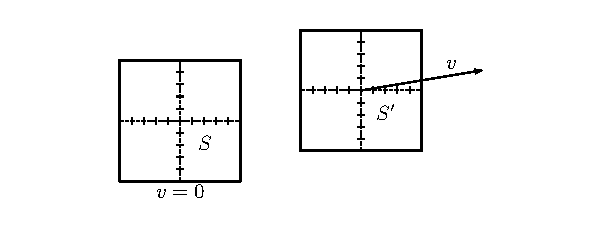
\includegraphics[width=4in, height=1.3in]{images/frames_in_motion.pdf}
			\caption{Frames $S$ and $S'$}
			\label{fig:frames-in-motion}
		\end{figure}

		In Galilean transformations, the relationship betwen the two reference
		frames can be described as 
		\begin{align*}
			x' &= x - vt\\
			t' &= t
		\end{align*}
		That is, expressed in matrix form, 
		\begin{equation}
			\bmqty{
				x'\\t'
			}
			= 
			\bmqty{
				1 & -v\\
				0 & 1
			}
			\bmqty{
				x\\t
			}
		\end{equation}
		This relationship is what is naively 
		assumed during day to day life, and in fact, it is
		readily apparent for observers without any knowledge of relativity. However,
		it has some issues. It implies that time $t$ is absolute, and, the reference frames
		$S$ and $S'$ are not strictly equivalent.
		
		As such, we need a more robust transformation. We seek the most general 
		transformation between the coordinates of the two frames.
		\begin{align}
		    x' = \overline X(x,t;v)\\
			t' = \overline T(x,t;v)
			\label{eq:general_transform}
		\end{align}
		The functions $\overline X$ and $\overline T$ are transformation functions that are initially unknown and undetermined.

		Our task, then, is to determine them from general physical principles. Simply 
		logic and mathematics, without any reference to experimental data whatsoever.
		This is, essentially, a purely mathematical approach. 

		Eventually, our goal
		is to obtain a transformation in the form of Lorentzian transfromations.

		\begin{equation}
			\bmqty{
				x'\\ t'
			}
			=
			\gamma
			\bmqty{
				1 & -\beta c \\
				-\beta/c & 1
			}
			\bmqty{
				x\\t
			}
		\end{equation}
		where $\gamma = \dfrac{1}{\sqrt{1-\beta^2}}$ and $\beta = \dfrac{v}{c}$

		An interesting question arises: Where does $c$ come from if we never assume light?

		\subsubsection{Principle of Relativity}

		The first assumption we make is Theorem \ref{thm:principle_of_relativity}, the principle of relativity.
		\begin{quote}
		    The laws of nature, that is, the laws of physics, take the same form in all inertial reference frames.
		\end{quote}

		In particular, $S$ and $S'$ are physically equivalent. There is no reason to regard 
		the transformation from $S$ to $S'$ as fundamentally different from the transformation 
		from $S'$ back to $S$.

		If $S'$ moves at velocity $v$ relative to $S$, then $S$ moves at a velocity $-v$ relative 
		to $S'$. Hence, the inverse transformation of (\ref{eq:general_transform}) must have the same functional form:
		\begin{align*}
		    x' = \overline X(x,t;-v)\\
			t' = \overline T(x,t;-v)
		\end{align*}

		This implies that if we apply the forward transformation followed by the inverse transformation, 
		we recover the original coordinates:
		\begin{equation}
			\begin{aligned}
				x &= \overline{X}\bigl(\overline{X}(x,t,v), \overline{T}(x,t,v), -v\bigr) \\
				t &= \overline{T}\bigl(\overline{X}(x,t,v), \overline{T}(x,t,v), -v\bigr)
			\end{aligned}
			\label{eq:composition-identity}
		\end{equation}

		\subsubsection{Isotropy of Space}

		The isotropy of space means that physics has no preferred direction. 
		In particular, the physics cannot distinguish between the $+x$ and $-x$ directions.
		This imposes the following:

		Consider reversing the spatial axis,
		\begin{equation}
			x\rightarrow -x.
		\end{equation}
		Under this reversal, the relative velocity also changes sign,
		\begin{equation}
			v\rightarrow -v.
		\end{equation}

		The spatial coordinate must therefore transform as
		\begin{equation}
			x'=-\overline X(x,t;v),
		\end{equation}

		while time, being a scalar under spatial reflection, satisfies
		\begin{equation}
			t'=\overline T(x,t;v).
		\end{equation}
		This distinction is important: $x$ changes sign under spatial reflection, but $t$ does not.

		Under time reversal combined with spatial reflection:

		\begin{equation}
			\begin{aligned}
				x' &= -\overline{X}(-x, t, -v) \\
				t' &= \overline{T}(-x, t, -v)
			\end{aligned}
			\label{eq:isotropy-conditions}
		\end{equation}

		For these to be consistent with the original transformations, we require:

		\begin{equation}
			\begin{aligned}
				\overline{X}(-x, t, -v) &= -\overline{X}(x, t, v) \\
				\overline{T}(-x, t, -v) &= \overline{T}(x, t, v)
			\end{aligned}
			\label{eq:parity-conditions}
		\end{equation}

	\subsubsection{The Invariance of Straight Lines}
		Free particles must move along straight lines in both frames. This is required
		by Newton's first law, the principle of inertia. In space time coodinates, we denote
		$x^\mu = (x,t)$\footnote{This is tensor notation, where $\mu$ identifies the component.
		In this 1+1 dimensional case, $x^1=x$ and $x^0 = t$. However, in general, $x^\mu=\bmqty{t,x,y,z}^\top$}
		and $x'^\mu = (x',t')$. Straight line motion in $S$ is therefore characterized by:
		\begin{equation}
			\dv[2]{x^\mu}{\tau} = 0 
		\end{equation}
		Where $\tau$ is some affine parameter\footnote{An affine parameter is an arbitrary parameter for which
		the geodesic equation is said to hold and takes the form of uniform motion without introducing artificial
		acceleration through the choice of parameter. i.e, affine parameters allow 
		reparametrization to be linear transformations. I don't understand it either, go figure. In this case, $\tau$ is called
		the \textit{proper time}}.

		The principle of inertia demands that straight lines map to straight lines.
		\begin{equation}
			\dv[2]{x^\mu}{\tau} = 0 \implies \dv[2]{x'^\mu}{\tau} = 0  
		\end{equation}
		The transformation from $S$ to $S'$ is represented in tensor notation as $x'^\mu = \overline{X}^\mu(x^\nu; v)$. Using the chain rule, with $x^\nu = x^\nu(\tau)$, we have:
		\begin{equation}
			\dv{x'^\mu}{\tau} = \sum_\nu \pdv{\overline{X}^\mu}{x^\nu} \dv{x^\nu}{\tau}
			\label{eq:chain-rule-first}
		\end{equation}
		Here, we impose the Einstein summation convention, where twice repeated indices are implicitly summed. 
		Explicitly:
		\begin{equation}
			\dv{x'^\mu}{\tau} = \pdv{\overline{X}^\mu}{x^0} \dv{x^0}{\tau} + \pdv{\overline{X}^\mu}{x^1} \dv{x^1}{\tau}
		\end{equation}
		Henceforth, we write this compactly as:
		\begin{equation}
			\dv{x'^\mu}{\tau} = \pdv{\overline{X}^\mu}{x^\nu} \dv{x^\nu}{\tau}
		\end{equation}
		with the understanding that $\nu$ is summed over its range. 

		Continuing the derivation, we have
		\begin{equation}
			\dv[2]{x'^\mu}{\tau} 
			= 
			\dv{}{\tau}\pqty{\pdv{\overline{X}^\mu}{x^\nu}} \dv{x^\nu}{\tau} 
			+ \pdv{\overline{X}^\mu}{x^\nu} \dv[2]{x^\nu}{\tau}
			\label{eq:chain-rule-second}
		\end{equation}
		The second term vanishes by the straight-line condition in $S$
		\begin{equation}
			\cancel{
			\dv[2]{x'^\mu}{\tau}}
		= 
		\dv{}{\tau}\pqty{\pdv{\overline{X}^\mu}{x^\nu}} \dv{x^\nu}{\tau} 
		+ \cancel{\pdv{\overline{X}^\mu}{x^\nu} \dv[2]{x^\nu}{\tau}}
		\label{eq:chain-rule-second-term}
		\end{equation}
		Therefore, from this result, we demand that the following relation must hold.
		\begin{equation}
			0 = \pdv[2]{\overline{X}^\mu}{x^\nu}{x^\sigma} \dv{x^\nu}{\tau} \dv{x^\sigma}{\tau}
			\label{eq:second-derivative-condition}
		\end{equation}
		For arbitrary velocities $\displaystyle\dv{x^\nu}{\tau}$,the quadratic form above must vanish for every possible velocity vector. this requires:
		\begin{equation}
			\pdv[2]{\overline{X}^\mu}{x^\nu}{x^\sigma} = 0
			\label{eq:linearity-condition}
		\end{equation}
		Therefore, $\overline{X}^\mu$ must be a linear function of the coordinates. Hence, we can write its components as:
		\begin{align*}
			\overline{X}(x,t,v) &= A(v)x + B(v)t + E(v)\\
			\overline{T}(x,t,v) &= C(v)x + D(v)t + F(v)
		\end{align*}
		These are just general equations of straight lines. 
	\subsubsection{Homogeneity of Spacetime}
		The next assumption we use is the homogeneity of space time.
		Spacetime homogeniety implies no preferred origin.

		Any point in both $S$ and $S'$ can be an 
		origin and spacetime would remain the same, so therefore we can choose the 
		location of the origin for both. 

		Therefore, we demand that the origin of $S$ gets mapped to the origin of $S'$ at $t=0$.
		\begin{equation}
			x = t = 0 \iff x' = t' = 0
		\end{equation}
		This is not really essential. However, it makes the derivation simpler and easier, since we can
		then set the constants $E(v)$ and $F(v)$ to zero. Doing otherwise would make the constant 
		terms indeterminable, which would increase the difficulty of the problem. However, the general
		result is the same. With this assumption, we can reduce our transformations to
		\begin{equation}
			\begin{aligned}
				\overline{X}(x,t,v) &= A(v)x + B(v)t \\
				\overline{T}(x,t,v) &= C(v)x + D(v)t
			\end{aligned}
			\label{eq:linear-no-constants}
		\end{equation}
		Thus, only four free functions of velocity  remain to be determined: $A(v), B(v), C(v),$ and $D(v)$.
		Our task, then, is to reduce these four free functions to just one function by exploiting properties
		that were previosuly shown. 

	\subsubsection{Parity Constraints}
		Applying the parity conditions from Eq.~(\ref{eq:parity-conditions}) to the linear forms, we have
		\begin{equation}
			\begin{aligned}
				\overline{X}(-x,t,-v) &= -\overline{X}(x,t,v) \\
				\overline{T}(-x,t,-v) &= \overline{T}(x,t,v)
			\end{aligned}
		\end{equation}
		This yields the following:
		\begin{equation}
			\begin{aligned}
				-A(-v)x + B(-v)t &= -A(v)x - B(v)t \\
				-C(-v)x + D(-v)t &= C(v)x + D(v)t
			\end{aligned}
			\label{eq:parity-linear}
		\end{equation}
		For these to hold for all $x$ and $t$, the following must be true
		\begin{equation}
			\begin{aligned}
				A(-v)&=A(v)\\
				D(-v)&=D(v)\\
				B(-v)&=-B(v)\\
				C(-v)&=-C(v)
			\end{aligned}
			\label{eq:parity-results}
		\end{equation}
		Thus, $A(v)$, $D(v)$ are even functions of $v$, and $B(v)$, $C(v)$ are odd functions of $v$
	\subsubsection{Inverse transformation and composition constraints}
		The inverse transformation from $S'$ to $S$ is
		\begin{equation}
		    \bmqty{
		    	x\\t
		    }
			=
			\bmqty{
				A(-v) & B(-v)\\
				C(-v) & D(-v)
			}
			\bmqty{
				x'\\t'
			}
		\end{equation}
		Explicitly,
		\begin{equation}
			\begin{aligned}
				x &= A(-v)x'+B(-v)t' \\
				t &= C(-v)x'+D(-v)t'
			\end{aligned}
			\label{eq:inverse-transform}
		\end{equation}
		Using the parity relations (\ref{eq:parity-results}),
		\begin{align*}
			x &= A(v)x'-B(v)t' \\
			t &= -C(v)x'+D(v)t'
		\end{align*}
		Substituting
		\begin{align*}
			x' &= A(v)x+B(v)t \\
			t' &= C(v)x+D(v)t
		\end{align*}
		to (\ref{eq:inverse-transform}), we obtain
		\begin{align*}
			x &= \phantom{-}A(Ax+Bt)-B(Cx+Dt) \\
			t &= -C(Ax+Bt)+D(Cx+Dt)
		\end{align*}
		Collecting coefficients we have,
		\begin{align*}
			x &= (A^2-BC)x + B(A-D)t \\
			t &= C(D-A)x + (D^2-BC)t
		\end{align*}
		Since $x$ and $t$ are arbitrary, the coefficients must satisfy
		\begin{equation}
		    \begin{aligned}
				A^2-BC&=1 \\
				B(A-D)&=0 \\
				C(D-A)&=0 \\
				D^2-BC&=1
		    \end{aligned}
			\label{eq:coefficient-conditions}
		\end{equation}
		So far, nothing specifically relativistic has appeared, there's no magic yet.
		We just used natural assumptions that come from geometry, and principle of relativity. 
	\subsubsection{The Trivial and Nontrivial Branches}
		The conditions
		\begin{align}
			B(A-D)&=0\\
			C(D-A)&=0
		\end{align}
		give us two cases.

		\paragraph{Case 1:} $A\neq D$

			If $A\neq D$, then, we are forced to conclude
			\begin{equation}
				B = C = 0
			\end{equation}
			The remaining equations give
			\begin{equation}
				A^2 = D^2 = 1
			\end{equation}
			Therefore,
			\begin{align*}
				A = \pm 1\\
				D = \mp 1
			\end{align*}

			Thus, the transformation becomes
			\begin{align*}
				x' &= \pm x\\
				t' &= \mp t
			\end{align*}
			This is a trivial transformation, corresponding to an identity/reflection type transformation
			rather than a continuosly varying boost between each reference frame. This is obvious. Of course, when you
			flip a frame, all the assumptions and constraints still hold. This is uninteresting.

			They are therefore not the nontrivial transformation we seek.
		\paragraph{Case 2:} $A=D$

			This is the nontrivial condition. The physically interesting case is therefore
			\begin{equation}
			A(v)=D(v).
			\end{equation}
			The condition
			\begin{equation}
				A^2-BC=1
			\end{equation}
			then gives
			\begin{equation}
				BC=A^2-1.
			\end{equation}
			provided that $B\neq 0$
			Thus:
			\begin{equation}
				C = \frac{A(v)^2-1}{B(v)}.
			\end{equation}
			We have reduced the four unknown free functions to two, since $A=D$, and once you know $A$ and $B$, you know C.
	\subsubsection{The motion of the origin of $S'$}
		Consider the motion of $S'$ through $S$.
		The spatial origin of (S') is defined by
		\begin{equation}
			x'=0
		\end{equation}

		Since $S'$ moves at velocity $v$ relative to $S$, its origin follows the trajectory
		\begin{equation}
			x=vt
		\end{equation}
		But every event on this trajectory must satisfy $x'=0$.
		Again, that is for the spatial origin. That means that entire \textit{worldline} needs to be mapped to $x' = 0$.
		
		Using 
		\begin{equation}
		    x' = Ax+ Bt
		\end{equation}
		we therefore have
		\begin{align*}
			0 
			&= Avt + Bt\\
			&= (Av + B)t
		\end{align*}
		Since this must hold for an arbitrary $t$, then
		\begin{equation}
		    B(v) = -v A(v)
		\end{equation}
		Now we only have one free function, $A(v)$.

		Consequently, we have
		\begin{equation}
		    C = \frac{A^2(v)-1}{vA(v)} 
		\end{equation}
		Thus, we have reduced the transformation to the following
		\begin{equation}
			\bmqty{
				x'\\t'
			} =
			\bmqty{
				A & -vA \\[4pt]
				- \dfrac{(A^2-1)}{vA} & A
			}
			\bmqty{x\\t}
		\end{equation}

		Now we only need to know $A$, except we dont know what properties of $A$ is.
		The only thing we can say for now is that matrix needs to reduce to the identiy matrix when $v = 0$

		Thus we impose
		\[
			A(v)\to 1,\quad v\to 0. 
		\]

		Since the $\tensor{M}{^1_0}$ term is a fraction with $v$ in the denominator, it must vanish sufficiently fast.
		therefore, $A^2 - 1 \approx \order{v^2}$
	\subsubsection{Introduction of a Third Observer}
		\label{subsubsec:3Intro3rdObserver}
		Consider a third inertial frame $S''$.

		Suppose $S''$ moves with constant velocity $u$ relative to $S'$, while $S'$ moves with
		constant velocity $v$ relative to $S$.

		It's the same framework, then. The transformation from $S'$ to $S''$ takes a similar form
		as from $S$ to $S'$. Let $M$ be a matrix such that 
		\begin{equation}
			\tensor{M}{^\mu_\nu}(v) = 
			\bmqty{
				A(v) & -vA(v) \\[4pt]
				- \dfrac{(A(v)^2-1)}{vA(v)} & A(v)
			}
		\end{equation}
		We can therefore denote the transformation from the $S$ frame to the $S'$ frame to be
		\begin{equation}
			x'^\mu = \tensor{M}{^\mu_\nu}(v) x^\nu
		\end{equation}
		Since the transformation is the same, then the transformation from $S'$ to $S''$ is
		\begin{equation}
			x''^\mu = \tensor{M}{^\mu_\nu}(u) x'^\nu
		\end{equation}
		Suppose that $S''$ is moving at a speed $w$ relative to $S$. Then
		\begin{equation}
			x''^\mu = \tensor{M}{^\mu_\nu}(w) x^\nu
		\end{equation}
		However, we demand the closure of transformations under composition. i.e, the form of the transformation is the 
		same, just with a different argument.
		Then, the transformation from $S$ to $S''$ is obtained by composing the two transformations from the intermediate reference
		frame.
		\begin{equation}
			x''^\mu = \tensor{M}{^\mu_\nu}(u)\tensor{M}{^\nu_\sigma}(v) x^\sigma
		\end{equation}
		That is, the form of the transformation from $S$ to $S''$ is the same form as the transformations
		from the other frames of reference.
		\begin{equation}
			\tensor{M}{^\mu_\sigma}(w) = \tensor{M}{^\mu_\nu}(u)\tensor{M}{^\nu_\sigma}(v)
		\end{equation}
		The crucial requirement is that the composition of two allowed transformations must itself be an allowed transformation.
	\subsubsection{The Emergence of an Invariant Speed}
		\label{subsubsec:emergenceinvariantspeed}
		We evaluate the composition by doing matrix multiplication.
		\begin{equation*}
			\tensor{M}{^\mu_\nu}(w) = 
			\bmqty{
				A(u) & -uA(u) \\[4pt]
				- \dfrac{(A(u)^2-1)}{uA(u)} 
					 & A(u)
			}
			\bmqty{
				A(v) & -vA(v) \\[4pt]
				- \dfrac{(A(v)^2-1)}{vA(v)} 
					 & A(v)
			}
		\end{equation*}
		Therefore, we have
		{\scriptsize
			\begin{equation*}
			\tensor{M}{^\mu_\nu}(w) = 
			\begin{bmatrix}
				A(u)A(v) + \dfrac{uA(u)\bigl(A(v)^2-1\bigr)}{vA(v)} & 
				-(u+v)A(u)A(v) \\[14pt]
				-\dfrac{\bigl(A(u)^2-1\bigr)A(v)}{uA(u)} - \dfrac{A(u)\bigl(A(v)^2-1\bigr)}{vA(v)} & 
				A(u)A(v) + \dfrac{vA(v)\bigl(A(u)^2-1\bigr)}{uA(u)}
			\end{bmatrix}
			\end{equation*}
		}
		By the nature of $M$, we see that the diagonal elements of the transformation matrix
		are equal, $\tensor{M}{^0_0}=\tensor{M}{^1_1}$. Therefore, we require the 
		equality of the elements. We equate:
		\begin{equation}
			A(u)A(v) + \dfrac{uA(u)\bigl(A(v)^2-1\bigr)}{vA(v)} 
			=
			A(u)A(v) + \dfrac{vA(v)\bigl(A(u)^2-1\bigr)}{uA(u)}
		\end{equation}
		Simplifying, we find that

		\begin{equation*}
			\cancel{A(u)A(v)} + \dfrac{uA(u)\bigl(A(v)^2-1\bigr)}{vA(v)} 
			=
			\cancel{A(u)A(v)} + \dfrac{vA(v)\bigl(A(u)^2-1\bigr)}{uA(u)}
		\end{equation*}
		\begin{equation}
			\dfrac{uA(u)\bigl(A(v)^2-1\bigr)}{vA(v)} 
			=
			\dfrac{vA(v)\bigl(A(u)^2-1\bigr)}{uA(u)}
		\end{equation}
		\begin{equation}
			\dfrac{\bigl(A(v)^2-1\bigr)}{v^2A^2(v)} 
			=
			\dfrac{\bigl(A(u)^2-1\bigr)}{u^2A^2(u)}
		\end{equation}
		The left hand side only depends on $u$, and the right hand side only depends on $v$.
		Since $u$ and $v$ are arbitrary, both sides must equal a universal constant.

		Let that constant be $k$:
		\begin{equation}
		    \frac{A^2(v) -1}{v^2A^2(v)} = k
		\end{equation}
		Rearranging, we have
		\begin{align*}
			A^2(v) - 1 & = kv^2A^2(v)\\
			A^2(v)(1-kv^2) & = 1
		\end{align*}
		Therefore,
		\begin{equation}
			A = \frac{1}{\sqrt{1 - kv^2}} 
		\end{equation}
		where we choose the positive branch because the transformation must 
		continuously approach the identity as $v\to 0$, thus reducing to the Galilean limit.
		\begin{equation}
		    A(0) = 1
		\end{equation}
		Note the units of $k$. For $A$ to be dimensionless, it has to have units which are $[L^{-2}][T^2]$, i.e, the inverse 
		of the units of the square of velocity.

		Now, notice that $M_{10}$ reduces to
		\begin{equation}
		    \frac{A^2 - 1}{vA} = kvA 
		\end{equation}
		
		Thus the transformation becomes
		\begin{equation}
			\bmqty{
				x'\\t'
			}=
		    A 
			\bmqty{
				1 & -v \\
				-kv & 1
			}
			\bmqty{
				x\\t
			}
		\end{equation}

		Equivalently,
		\begin{align}
			x'
			&=
			\frac{x-vt}{\sqrt{1-kv^2}}
			\\[4pt]
			t'
			&=
			\frac{t-kvx}{\sqrt{1-kv^2}}
		\end{align}

		This are already the Lorentz transformations in generalized form.

		From this, we can derive that\footnote{To be proven.}
		\begin{equation}
			w = \frac{u+v}{1 + kuv} 
		\end{equation}
		This is the familiar relativistic velocity addition formula. 

		Writing $k$ always in terms of $1/k^2$ is a bit cumbersome, especially when writing longer proofs.
		We hereby assign a new symbol for the speed.
		Let $\kappa = \frac{1}{\sqrt{k}}$.

		Suppose we set $u = \kappa$. Then, we find
		\begin{equation}
		    w = \frac{\kappa + v}{1+kv\kappa} 
		\end{equation}
		Since $k\kappa = \dfrac{1}{\kappa}$, we then obtain
		\begin{align*}
			w &= \frac{\kappa + v}{1 + \frac{v}{\kappa}} \\
			  &= \frac{\kappa + v}{(\kappa + v)/\kappa} \\
			  &= \kappa
		\end{align*}
		thus:
		\begin{equation}
		    u = \kappa \implies w = \kappa
		\end{equation}
		The speed $\kappa$ is therefore invariant under the velocity-composition law. 

		This is the crucial result from all that derivation.
		The principle of relativity does not tell us what the invariant speed is. It 
		tells us that:
		\begin{theorem}{Universal Invariant Speed}
			\hspace{2em}For the Lorentzian branch of the kinematics, there must exist a 
			universal invariant speed $\kappa$.
		\end{theorem}
		\newpage	
	\subsubsection{The Relevance of Light}
		Where did light enter the discussion? It has not entered the argument at all. We only 
		began with the following fundamental principles
		\begin{enumerate}
		    \item principle of relativity
			\item homogeneity of space
			\item homogeneity of time
			\item isotropy of space
			\item principle of inertia
			\item closure of transformations under compositions
		\end{enumerate}
		and these assumptions led us to find the transformation equations. Nowhere did 
		Maxwell or electromagnetics come into the picture.

		We did not need light at all. In this sense, the theory of relativity is derived
		and works on pure mathematical logic alone. All of physics bows down to this principle.

		The empirical question that can then be raised is: Which value $k$ describes our universe?

		Experiment tells us that the invariant speed is the speed of light in a vacuum.
		\begin{equation}
		    \kappa = c
		\end{equation}
		so that
		\begin{equation}
		    k = \frac{1}{c^2} 
		\end{equation}
		It did not need to be light. If we were more sensitive to gravitational waves,
		we would have called it thus. However, we are a species who evolved to sense light
		better, and it was this that lead us to stumble upon relativity. But there is in 
		fact no need at all for it. A a blind society, insensitive to light, just with principles and logic, can
		establish relativity. Thus, electromagnetism does not need to be used to \textit{derive} the Lorentz
		transformation. Instead, electromagnetism provides us an empirical way of identifying
		the invarient speed. 
		
		In this sense, light acts as a calibrator of the kinematics rather than as the logical 
		foundation of the transformation.
		
	\subsubsection{The Galilean Limit}
		There is another possibility.

		If we set $\kappa\to 0$, then $\kappa\to\infty$ and $A\to1$,
		the transformation thus becomes
		\[
		    \bmqty{
		    	x'\\t'
		    } =
			\bmqty{
				1 & -v \\
				0 & 1
			} \bmqty{
				x\\t	
			} 
		\]
		These are precisely the Galilean transformations. The corresponding 
		velocity addition law is then
		\[
			w = u + v
		\]
		In this case, the invariant speed is effectively infinite. Thus, Galilean relativity can 
		be viwed as the $\kappa \to \infty$ limit of the generalized transformation.
	\subsubsection{Lorentzian, Galilean, and Carrollian kinematics}
		The parameter $k$ therefore distinguishes different possible kinematic structures.

		For $k>0$, there is a finite invariant speed
		\[
			\kappa = \frac{1}{\sqrt{k}} 
		\]
		giving us Lorentzian relativity.

		For $k=0$, the invariant speed becomes infinite, giving Galilean relativity.
		The main reason that Galilean relativity took hold for so long is for quite some 
		time in the enlightenment, people thought that the speed of light is infinite, 
		and so that is the logical conclusion.

		While inaccurate at relativistic scales, Galilean relativity, and by extension 
		Newtonian physics, remains central to physics education because, for systems 
		involving velocities $v\ll c$ and ordinary spatial and temporal scales, it provides
		an excellent approximation to relativistic physics. In this regime, the corrections
		predicted by special relativity are negligible, making the Galilean description both 
		sufficiently accurate and considerably simpler as a description of reality.

		There is also a limiting case in which the invariant speed tends to zero. As $k\to\infty$,
		\begin{equation}
		    \kappa \to 0
		\end{equation}
		This is associated with the Carrolian limit of relativity.
		In this regime, the causal structure becomes increasingly restrictive: events 
		at distinct spatial locations cannot influence one another within any finite
		time interval, and the notion of spatial propagation effectively disappears. 
		The resulting Carrollian kinematics therefore describes a theory in which particles 
		may evolve in time while remaining effectively frozen in space, providing the 
		opposite extreme to the Galilean limit of instantaneous propagation.

		These three structures can therefore be understood schematically with light cones,
		representing the travel of information in an observer's frame of reference.
		\begin{figure}[h]
			\centering
			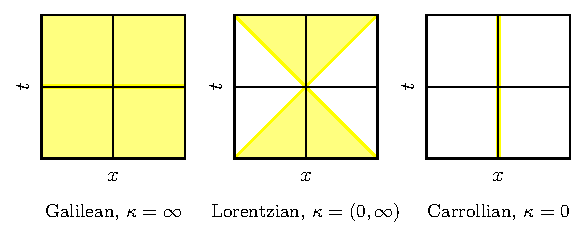
\includegraphics[width=4in]{images/cones_types_of_relativity.pdf}
			\caption{Light cones in different types of relativity}
			\label{fig:cones-types-of-relativity}
		\end{figure}

		The light cone structure which posits finite travel of information belongs to 
		the finite Lorentzian case. The causal cone has a finite opening angle because 
		there is a finite maximum invariant speed. In the Galilean limit, the cone opens 
		out to incompass instantaneous propagation of information, no matter the distance
		of the interaction. In the Carollian limit, the cone collapses, corresponding to
		the extreme opposite situation where spatial propagation, and travel of information,
		is suppressed, no matter now much momentum a particle carries. As such a body can 
		only travel forwards in time, fixed in the same space, with no information reaching it.
		Such a universe would be mathematically interesting, but in effect, it is a dead universe.

	\subsubsection{Conclusion}
		This, and this is a point that I will not get of tired telling you,\footnote{Actual verbatim quote from sir}
		proves the point that the derivation of the Lorentz transformation does not logically require 
		the existence of light. The transformation
		\[
			\bmqty{
		    	x'\\t'
		    } =
			\gamma
			\bmqty{
				1 & -v \\
				-\beta & 1
			} \bmqty{
				x\\t	
			} 
		\]
		can be obtained from the structure of inertial frames and the relativity principle alone, 
		with the constant $c$ initially appearing simply as an arbitrary invariant speed. Experiment
		then tells us that this invariant speed is 
		\begin{equation}
			c = \SI{299792458}{m/s}
		\end{equation}
		and that electromagnetic wave propagation also happens to have an invariant speed, and that speed turned out
		to be $c$ as well, for electromagnetic radiation travel precisely this speed in a vacuum.

		The logical relationship can be summarized as 
		\[
			\text{Relativity}\implies\text{possible invariant speed } \kappa
		\]
		while experiment establishes
		\[
			\kappa = c
		\]
		Electromagnetism therefore provides an empirical realization of the invariant speed; 
		it is not necessary as a premise in the kinematic derivation itself.
		The deeper lesson is that the Lorentz transformations and relativity itself is fundamentally a statement about 
		the symmetry of spacetime, not specifically about light.
		\begin{remark}
			Some points because I wasn't able to elaborate on them. $\overline{X}^\mu(x^\nu)$ is simply 
			the tensor packaging of the transformation functions, where $\overline{X}^0(x^\nu;v) = \overline{X}(x,t;v)$
			and $\overline{X}^1(x^\nu;v) = \overline{T}(x,t;v)$. It is a vector valued function. Whereas $\tensor{M}{^\mu_\nu}$
			is a matrix. Once linearity is proven, we can show that $\tensor{M}{^\mu_\nu}$ is a Jacobian, related to $\overline{X}^\mu$
			by
			\[
				\tensor{M}{^\mu_\nu} = \pdv{\overline{X}^\mu}{x^\nu} 
			\]
		\end{remark}	
		\newpage
		\subsubsection*{Addendum}
			In \S \ref{subsubsec:emergenceinvariantspeed}, we are given the velocity addition formula
			\[
				w = \frac{u+v}{1+kuv}
			\]
			and told it is true without proof, despite being pivotal to the proof that there is
			an invariant speed that arises in Lorentzian mechanics.

		    This wasn't elaborated in the lecture for time constraint reasons, as Sir was rushing to finish the 
			invariant speed derivation before class dismissal, and thus it was left as an exercise to the student. 
			Finding no satisfaction in it being simply stated as true, I took the liberty of proving the relation.
			\begin{proof}
				From \S \ref{subsubsec:3Intro3rdObserver}, we know that the origin of the second frame
				$S''$ has velocity
				\begin{equation}
					\label{eq:wterm}
					w = \dv{x}{t} 
				\end{equation}
				as measured from $S$.

				The same reference frame has velocity
				\[
					u = \dv{x'}{t'} 
				\]
				as measured from $S'$. 

				We also know that $S'$ travels at a velocity $v$ relative to $S$.
				We aim to determine $w$ in terms of $u$ and $v$. 

				From the generalized Lorentz transformation,
				we have the transformed coordinates in $S'$
				\begin{align*}
					x' = \frac{x - vt}{\sqrt{1-kv^2}} && t' = \frac{t-kvx}{\sqrt{1-kv^2}}`` 
				\end{align*}
				Taking the differentials of these equations give
				\begin{align*}
					\dd{x'} = \frac{\dd{x}-v\dd{t}}{\sqrt{1-kv^2}} && \dd{t'} = \frac{\dd{t}-kv\dd{x}}{\sqrt{1-kv^2}}  
				\end{align*}
				Hence, we have
				\begin{align*}
					u &= \dv{x'}{x'}\\ &= \frac{\dd{x}-v\dd{t}}{\dd{t}-kv\dd{x}}  
				\end{align*}
				We divide both the numerator and denominator by $\dd{t}$, we have
				\begin{align*}
					u &= \frac{\displaystyle\dv{x'}{t}}
					{\displaystyle\dv{t'}{t}} \\[10pt]
					  &= \frac{\displaystyle\dv{x}{t} - v\dv{t}{t}}
					          {\displaystyle\dv{t}{t} - kv \dv{x}{t}}  
				\end{align*}
				Since we know that (\ref{eq:wterm}), and $\displaystyle\dv{t}{t}=1$, then we obtain.
				\begin{equation}
					u = \frac{w-v}{1-kvw} 
				\end{equation}
				Solving for $w$, we find that
				\begin{align*}
					u(1-kvw) &= w-v\\
					u - kuvw &= w-v\\
					u + v &= w + kuvw\\
					u + v &= w(1+kuv)\\
					w &= \frac{u+v}{1+kuv} 
				\end{align*}
				Therefore, the velocity of $S''$ relative to $S$ is:
				\begin{theorem}{Relativistic Velocity Addition}
					\begin{equation}
						w = \frac{u+v}{1+kuv} 
					\end{equation}
				\end{theorem}
			\end{proof}

		\newpage
	\chaptersec[Aspects of Differential\\Geometry]
	           {Aspects of Differential Geometry}
		% =======================================
% MEETING 4
% ---------------------------------------
% DATE   - AUGUST 28, 2026
% FORMAT - ONLINE
% =======================================
% TOPIC  - MANIFOLDS AND TOPOLOGICAL SPACES
% =======================================


\subsection{Manifolds and Topological Spaces}

	\textit{This lecture was conducted online due to weather constraints, and so I had time to pause and rewind the lecture. Thus, most of what is written here is verbatim.}

	Last meeting, we discussed that relativity
	functions without the need of light, and derived the equations
	of SR without any assumptionss pertaining to light and assumptions
	that were more natural coming from established or logical 
	principles. 

	What we will learn in subsequent lectures is that SR, at least
	in the way we understand it now, is really about physics in 
	Minkowski spacetime. 

	And so, we will discuss what spacetime is today, and one of the foundational
	concepts in understanding spacetime is the notion of manifolds.
	So today, we shall start talking about manifolds. This is gonna be a very
	lightning quick introduction to manifolds.

	So why manifolds? Why are they important? Before we get to manifolds, let's first understand
	what spacetime actually is, and what are topological spaces and other preliminaries.

	\subsubsection{Spacetime}
		Spacetime, in an intuitive sense, is just a collection of all \textit{events} in physics. 
		An event is just a \textit{here} and a \textit{now}, so you can think 
		of spacestime as a here and a now. It's very intuitive, the way a philosopher
		might want to describe it. Spacetime, as we understand it, is just\footnote{we say just because this was how it was conceived back in the olden times}
		the background on which physics takes place. The stage, so to speak. 

		It's hard to imagine physics without actually thinking about events. Say, for example, an electromagnetic field,
		there's always some kind of field vector, like an electric field vector or a magnetic field vector
		existing at some spatial point and some instant of time. We think about some sort of arrow
		existing on some kind of background, traditionally $\R^3 + t$, and that's what we think 
		spacetime is. There is always spacetime, there has always been space and time in physics,
		but for most cases, we didn't give it much thought, right? It was simply a stage at which
		physics happens, and where particles and fields effectively \textit{play}. 

		However, modern physics is different. In fact, in some sense, this is a \textit{characteristic} of 
		modern physics, we have to take into account the role played by spacetime because spacetime
		is not just some inert object anymore, in general relativity in particular, because in fact all
		modern relativistic theories have to contend with the empirical fact that spacetime does have
		dynamical role serving a stage for everything else.

		Modern physics requires us to be careful of this \textit{stage}, because it participates 
		greatly in how reality behaves. In particular, we have to be careful about the structures which
		live on this stage. 

		So what am I talking about here, what \textit{structures}? These are structures that we are 
		all familiar with, such as scalars, vectors, and there will be a spinors sometiems, one forms,
		but in general, all of these will be subsumed by what we know to be tensors. So all these objects
		are the objects that can naturally live on space time. We want these to be the things that represent
		the physical objects that we're used to, such as fields and particles, and we need a mathematical
		structure which can contain or allow the existence of these objects and this will turn out 
		most naturally to be a manifold. 

		Before relativity, as I've explained in previous lectures, the implicit assumption that
		there was some kind of background that was just plainly Euclidean. Pre-relativity, before
		Einstein's time, there was just the Newtonian picture. For example there was already
		a space time in those times, a space structure and a time structure. Here, it's probably
		not very appropriate to join space and time, because it was really space \textit{and} time,
		to have a Euclidean structure, at least a Euclidean structure for space. In fact, it was a 
		very specific kind of space time, it was a manifold\footnote{which is what we generally call what a spacetime is}
		\begin{equation}
			\label{eq:manifold}
				\mathcal{M} = \R\cross\R^3
		\end{equation}
		In other words, it had the familiar Euclidean space $\R^3$ for space and time. So you can sort of 
		visualize it as something like this

		\begin{figure}[h]
		    \centering
		    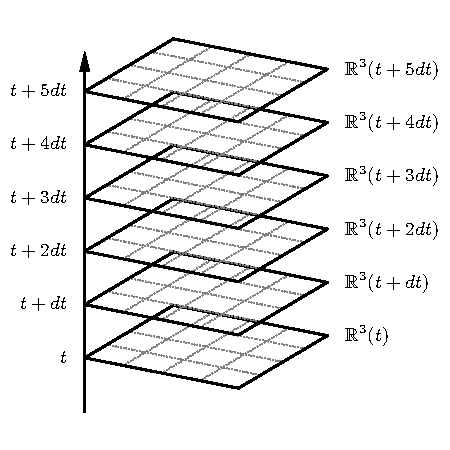
\includegraphics[width=3in,height=3in]{images/prerelativityspacetime.pdf}
		    \caption{Conception of space time before relativity}
		    \label{fig:prerelativityspacetime}
		\end{figure}
		
		So each point in time $t$ (which is a real line $\R$), which is absolute global universal time, there is an associated copy of $\R^3$.
		Time is going forward, and space is \textit{coupled} to each point in time, and there would be a 
		particle going through this space time. This was the structure of pre-Relativity physics, This was
		before Minkowksi. Bear in mind that this is not Euclidean $\R^4$, but simply distinct $\R$ and $\R^3$ structures.

		Furthermore, for this Euclidean space, there is also an assumed distance metric, which
		measures the distances between points in $\R^3$. For Euclidean space, this is basically the distance formula.

		\[
			d(u,v) = \sqrt{\sum_i(u_i - v_i)^2},\qquad u,v\in\R^n
		\]

		But in the modern conception of spacetime, it has to be far more general, in recognition
		of the insights of Einstein and many others. So, we'll provide a more modern definition. In fact,
		there are several definitions of spacetime, they all roughly correspond to the same thing. Some
		are just more careful because some are more mathematically oriented. But I shall provide two
		definitions just for your reference. The first one is by Sasane\cite{Sasane2021}, he was a mathematician 
		interested in relativity. 

		\begin{definition}{Spacetime (Sasane)}
		Spacetime, ($\mathcal{M},g$) is a connected four dimensional, oriented (time oriented)
			Lorentzian manifold $\mathcal{M}$ with metric $g$, equipped with a Levi-Civita connection,
			induced by $g$, together with a time orientation.
		\end{definition}

		There are a couple of things we should take note of here. Notably, there are terms like \textit{connected}, which
		we'll explain in due course. \textit{Four dimensional}, which more or less we have a notion of, and there is a 
		\textit{manifold}, which we're going to talk about today. There is the term \textit{Lorentzian}, which actually
		refers to the metric $g$, and there's also a notion of the \textit{Levi-Civita connection}, and somehow
		this Levi-Civita connection is supposed to come from $g$, presumably. What this means is that if there
		is a metric $g$, it implies a Levi-Civita connection. And we have \textit{time orientation}. All of these terms,
		we will have to parse in the days ahead. 

		The more classic definition of spacetime comes from the great Hawking and Ellis\cite{HawkingEllis1973},\footnote{If you are particularly interested in understanding relativity from a mathematical point of view, I will highly recommend Hawking and Ellis as a book, but not as a first textbook. There are still aspects of Hawking and Ellis that are a bit difficult for me to understand, but this has been  a standard reference for some time.}
		The definition they provide is a little bit simpler than Sasane's which is more modern, they say that
		\begin{definition}{Spacetime (Hawking and Ellis)}
			Spacetime is the collection of all events, represented by a pair $\mathcal{M},g$, where $\mathcal{M}$ is a connected
			four dimensional Hausdorff $C^\infty$ manifold and $g$ is a Lorentz metric
		\end{definition}
		There are some common elements, such as the terms \textit{connected} and \textit{four dimensional}. There is a topological
		feature here: \textit{Hausdorffness}. This is a separability assumption, we will discuss this in a bit. And then there is a 
		notion of a $C^\infty$ manifold, which we will discuss today as well, and then there is a Lorentz metric and $g$, both 
		definitions pertain to the same thing, which we will make sense of in the days ahead. 

		First we discuss the $C^\infty$ manifold, or manifolds in general.

	\subsubsection{Manifolds}
		Those definitions discuss both an $\mathcal{M}$ manifold and a $g$ metric. As such, we discuss what is a manifold. 
		First, I will write down what I consider to be a sufficient definition for what a manifold is, and then I'll give 
		you my own take of how do you make sense of a manifold, from an intuitive point of view. 

		\begin{definition}{Manifold}
			An $n$-dimensional differentiable or smooth manifold\footnote{In this class when we talk about manifolds we always mean differentiable or smooth manifold} $\mcal M$
			is a topological space with open cover\footnote{If you take the union of all these open sets then it gives you the whole manifold} 
			$\qty{\mathcal{O}_\alpha}$ (i.e., $\mathcal M = \cup_\alpha \mathcal{O}_\alpha$)
			and charts $\qty{(\psi_\alpha, \mathcal{O}_\alpha)}$ such that each $\psi_\alpha$ is a homeomorphism and if $\mathcal{O}_\alpha \cap \mathcal{O}_\beta\neq\varnothing$, the composite map $\psi_\beta \circ \psi_\alpha^{-1}$ is
			$C^\infty$ (or smooth).
		\end{definition}

		The gist is that a differentiable manifold or a smooth manifold is something that is 
		coordinatizable. So from a physicist's standpoint, that's a way to understand what a manifold is.  An $n$-dimensional manifold is a topological space 
		that is locally homeomorphic to $\R^n$, together with appropriate compatibility within charts. It has the local differential structure of $\R^n$ but not necessarily its global properties.

		\newpage %remove if able
		In short: A manifold is basically a topological space on which you can install coordinates in. It is a topological
		space which is coordinatizable.

		So, obviously there are numerous examples when you need coordinatizability and it's very  difficult to actually imagine
		situations in fundamental physics in which there are no coordinates, and there are many examples of these manifolds in physics,
		in fact manifold structures
		are implicit for most branches of physics. For those branches of physics you don't need to be very careful
		about what the manifold  is, so long as you're using coordinates to describe your physics. However, if you need to place
		coordinates in your physics, you need the structures given by manifolds.

		For example, Thermodynamics, so when you think about the state spaces there, coordinatized by, say $P_V T$, for instance, 
		thermodynamic variables, those are examples of manifolds. When you're doing mechanics, for example, you deal with phase spaces,
		phase spaces typically have coordinates that you can configure, such as $q_\alpha$ and $p_\alpha$, those are also manifolds.

		Any application or situation, where you have coordinates, you implicitly use manifolds. The important point is that in GR, or relativity, we have to be careful
		about the manifold and not just be so focused on the coordinates because the coordinates are just things that live on top of a 
		manifold. 

		I'm hoping that's clear, but we'll make that even clearer in a bit.

		\begin{figure}[h]
			\centering
			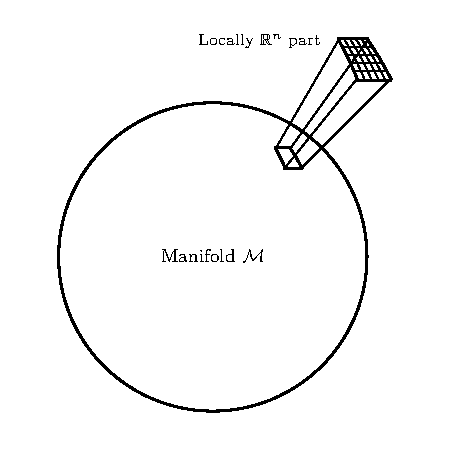
\includegraphics[width=3in]{images/manifold_ex1.pdf}
			\caption{Manifold example}
			\label{fig:manifoldex1}
		\end{figure}
		Aside from being locally coordinatizable, it is also always\footnote{i.e., every point has a neighborhood homeomorphic to an open subset of $\R^n$} locally $\R^n$. 

		In other words, if a manifold exists (Fig \ref{fig:manifoldex1}), and you take a small part there, that small part of it will always have a set of $n$ coordinates. That is, a set of $n$ numbers describe the members of the set, that's
		what it means. Locally $\R^n$ just means that you can always find $n$ numbers to completely describe the elements of any set $\mathcal{O}_\alpha$. 
		But before we get to that, now we talk about topological spaces; this is gonna be another very lightning quick review of what
		a topology is, because this is not a mathematical methods class, this is really a GR class but we have to say a little bit about it.

	\subsubsection{Topological Space}
		A topological space is just a set with a topology. What is a topology? A topology on a set $\mathcal M$ is a collection $\mathcal T$ of subsets of $\mathcal M$, called open sets, satisfying three axioms defined below. 
		In other words, a topology is an abstract specification of what is called open balls or open sets, usually $\R^n$, denoted by \textit{the set of open sets}, $\qty{\mathcal{O}_\alpha}$.
		If you have a set $\mcal M$, you can identify subsets of that set, and call it open sets.
		But you can't just name any subset to be an open set, they have to satisfy certain
		rules or criteria. These criteria are:
		\begin{enumerate}[(1)]
			\item The set $\mathcal{M}$ and the null set $\varnothing$ are both open. 
				\[
					\mathcal{M},\varnothing\in\qty{\mathcal{O}_\alpha}
				\]
				Since $\qty{\mathcal{O}_\alpha}$ is defined as the set of all open sets, we require in the specification of open set that $\mcal{M}$, the full set,
				and the empty set $\varnothing$, are both elements of the set of open sets.
			\item If you take an arbitrary union of open sets, it must also be open
				\[
					A_i \in \openset\implies \bigcup_i A_i \in \openset
				\]
				For example, you already specified the open sets in the set, and you take the any union of any of those things you named in the open set, their union 
				must also be open. It holds regardless of how many unions of sets you take. It must also be an element of $\qty{\mathcal{O}_\alpha}$
			\item Finite intersections of open sets must be open. 
				\[
					A_1, A_2,\ldots, A_n \in \openset\implies \bigcap_{i=1}^n A_i \in \openset
				\]
				for any positive integer $n$.

				That is, for any open set you define, the finite intersection of how many such sets you take, must also be open. The \textit{finite} restriction in 
				this case is crucial.
		\end{enumerate}
		That's it, that's all we need to define an open set. I'll give you a very easy example, it's very trivial, it's hardly useful but it's good for understanding 
		definitions, it's what's known as the indiscrete topology. 
		\paragraph{Indiscrete Topology}

		In the indiscrete topology, we define that the only open sets are $\mathcal M$ and the null set $\varnothing$. 
		\[
			\qty{\mathcal{O}_\alpha} = \qty{\mathcal{M},\varnothing}
		\]	

		Is this a topology? Clearly it satisfies the first condition, by construction. The required members of the topology are already open sets by declaration.
		Does this satisfy the second criteria of arbitrary unions? Well, the only union you can take is between $\mathcal M$ and the empty set, and itselves, and as such:
		\begin{align*}
			\mcal{M} \cup \varnothing = \mcal M &&
			\mcal{M} \cup \mcal{M} = \mcal{M}&&
			\varnothing \cup \varnothing = \varnothing
		\end{align*}
		But $\mathcal M$ is already an open set by definition, as is $\varnothing$. Therefore, it satisfies the second criteria. What about finite intersections? Here, it is not really relevant
		because the open set is already a finite set with only two elements. Similarly, the only intersection we can take is 
		\begin{align*}
			\mcal{M} \cap \varnothing = \varnothing &&
			\mcal{M} \cap \mcal{M} = \mcal{M}&&
			\varnothing \cap \varnothing = \varnothing
		\end{align*}
		and all of these are already members of the set of open sets, so the third criteria is already satisfied. So this is an example, the simplest example, of a topology.
		You identify subsets, not necessarily proper subsets, but subsets of your set of open sets, and you call them open. It's a declaration of what the open sets in your set are. 
		
		This is what's known as the coarsest topology, because it only has two open sets. It is practically useless for application, but again it's good for understanding definitions.
		\paragraph{Discrete Topology}
		We also have what we call a discrete topology, which is the other side of spectrum. The discrete topology is the finest topology, since it says that all the subsets of the set 
		of all open sets are be open.
		\[
			\qty{\mcal{O}_\alpha} = \text{all subsets}
		\]
		So clearly, all three criteria are already satisfied, because all the subsets are defined to be open. So trivially, this is already
		a topology. But the problem with this is that it's too fine grained, and it's not exactly useful anywhere else. 
		That's a very rough sketch of what a topology is, let me tell you what topologies are used for.

		A topology on a set is essential for providing a notion of continuity of maps on the set. 

		This is the most important point. We normally have this naive, sort of intuitive understanding of what a continuous function is, this is already 
		distilled by mathematicians. So if you were to talk about an arbitrary set, what notion do you need for you to 
		define the continuity of functions on a set. 

		So in other words, say we have a map $f$
		\[
			f:M\to N
		\]
		if you say for example that $f$ is continuous map from $M$ to $N$, the assumption here is that, you cannot make sense of this unless
		$M$ and $N$ are topological spaces. This is already assuming that $M$ and $N$ to be topological spaces. In other words, they need to be sets 
		with a topology, i.e., both $M$ and $N$ have identifiable open sets that are subject to the conditions defined above.

		This is all a bit a abstract, but hopefully will induce you to try to learn more because, topology, in general, is taught over several semesters. So
		I'm just giving you a sense here of what it means, and because we need to define what continuity is, in order to grasp a 
		full understanding of what we need topological spaces for.

	\subsubsection{Continuity}
		The modern definition of continuity is this
		\begin{definition}{Continuity}		    
			In general, a map $f:M\to N$ is continuous if the preimage of $\mcal{O}$ belongs to the topology $\mcal{T}_1$, for all open sets in $\mcal{T}_2$, where $\mcal{T}_1$ is the topology on $M$ and $\mcal{T}_2$ is the topology on $N$
			\[
				f^{-1}[\mcal{O}]\in\mcal{T}_1,\ \forall \mcal{O}\in\mcal{T}_2
			\]
		\end{definition}
		What does this all mean? If you say \textit{the topology}, you don't mean just the set. Say the set $M$, it has the accompanying topology which is just a specification
		of open sets on $M$, then you have $N$, where you need to also specify what the open sets are (what you call $\mcal{T}_2$). The requirement then, for the map $f$ to 
		be continuous is that for all the sets that you take in $N$, its preimage, must also be open in $\mcal{T}_1$, or in $M$. This
		is the clearest way that it can be discussed which makes sure that you can understand that this is in fact identical to the notion of continuity in terms of open balls
		that is being discussed in calculus.

		Suffice to say, then, that the definition of continuity requires topologies to exist in both the domain and the codomain. 
		\begin{equation*}
			\begin{rcases}
				(M, \mathcal{T}_1) \\
				(M, \mathcal{T}_2)
			\end{rcases}
			\text{ Topological spaces}
		\end{equation*}
		The key point here is that without topology, there is no notion of continuity.
		Now this all sounds very abstract; I mean this is a fun subject, I actually like topology
		a lot, but for physics, it is usually enough to use open sets. 

		\paragraph{What is a preimage?} 
			The preimage is kind of like the inverse of a function. For example, say that $f$ is a function which maps the domain $M$ to the codomain $N$ (Fig. \ref{fig:preimagedefinition}). The
			preimage means that if you take any set in $N$, say $\mcal{O}$, then the preimage of $\mcal{O}$ is all the elements on $M$ that when $f$ is applied, will be mapped to $N$. So,
			in essence, it's like the inverse function.
			The inverse of $f$ need not exist, but the preimage will always exist. So there are a bunch of points in $M$, call them $\mcal W$, that will be mapped entirely to $\mcal O$ by $f$. Those sets of points
			is the preimage of $\mcal O$. i.e., $f(f\inv[\mcal O]) = \mcal O$
			\[
				f^{-1}[\mcal O] = \qty{x\in M : f(x)\in \mcal O}
			\]
			\begin{figure}[h]
				\centering
				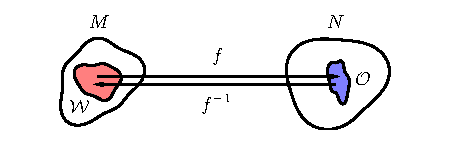
\includegraphics[width=3in,height=1in]{images/preimage.pdf}
				\caption{Pre-image of $\mcal{O}$, $ \mcal{W}=f^{-1}[\mcal{O}]$ and $\mcal{O} = f[\mcal{W}]$}
				\label{fig:preimagedefinition}
			\end{figure}
		\paragraph{Usual examples of Topologies}
			We already discussed many weird examples like indiscrete and discrete topologies. However, there
			are more usual topologies. These are the so-called \textbf{Open ball topologies}, the standard
			topology in $\R^n$. Some examples are
			\begin{enumerate}[(1)]
			    \item $\R$

					  The real line is an example of an open topology. It has open intervals as its open sets; this is the standard 
					  Euclidean topology. Such examples are the set of numbers from $x$ to $y$ in the real line:
					  \begin{align*}
						  (x,y),\quad x<y,\quad x,y \in \R
					  \end{align*}
					  These are the open sets. Therefore, the set of open sets of $\R$ is
					  \[
						  \openset = \qty{\cup_\alpha(x_\alpha,y_\alpha): x_\alpha<y_\alpha}
					  \]
					  These are the open intervals which define a topology. You can check this using the three criteria: $\R$ is open $(-\infty,\infty)$, any union
					  of open intervals is still open, and any finite intersections of open intervals in the real line is also open. Therefore, these sets form a topology on $\R$.
					  \begin{remark}
						  Finite here is important, because you can imagine a construction of sets, say $\qty{\frac{1}{n},1},\ n\in\N$, these are all individually open, this is a subset 
						  of all possible intervals from 0 to 1. If you take an infinite intersection of this interval, $1/n$ will eventually converge (limit) to zero, hence:
						  \[
							  \bigcap_n^\infty \pqty{\frac{1}{n},1} = [0,1)
						  \]
						  Then it is no longer open. For larger and larger $n$'s, the result will include $0$, so it will longer be 
						  open, that's why you need the intersections to be finite. That's the standard topology in $\R$. In fact, 
						  you can also define a topology using closed intervals, that's also an interesting exercise.
					  \end{remark}

				\item $\R^n$ 

					  Typically, in general $\R^n$, we use open balls $B_r$ with radius $r$. 
					  \[
						  B_r(\vb x) \equiv \qty{\vb y : \abs{\vb{x}-\vb{y}} < r}
					  \]
					  That is, all the points $\vb y$ with a distance from $\vb x$ less than $r$, a \textit{ball} which has open intervals, is an open 
					  set.

					  If you declare that your open sets are open balls in $\R^n$, you recover the so-called standard topology as well. 
					  Similar to the arguments for $\R^1$, we can also show that all of $\R^n,\ n\in\Z$ to be topologies. It has a name, called
					  Euclidean topologies.
			\end{enumerate}
			There's a lot to study here, but we're not going to need all of topology, it's sufficient to know what a topology is and why it's important
			for our understanding of a manifold. 

			So again, what is a topology? It's just a set and a specification of open sets of the set. That is, $\mcal M$ and the open sets of $\mcal M$. 

			Going back to the definition of a manifold, it is a topological space with an open cover $\openset$, these are just the open sets
			I talked about, and also, we require that the union of all these open sets, it results to the full manifold set itself, $\mcal M$. 
			\begin{equation}
				\label{eq:union-of-opensets}
				\mcal{M} = \bigcup_\alpha \mcal O_\alpha
			\end{equation}
			There should be no element of the set that does not belong to an open set. For example, you start with a set $\mcal M$, and then you 
			declare open sets to be your topology. In that declaration, there should be no element or point in $\mcal M$ that is not part of an open set. That's
			the requirement for you to have an open cover. These sets of open sets need to satisfy the conditions for the criteria for a topological space.
		
			It has charts, which maps open sets to a subset of $\R^n$, and it is a homeomorphism. Homeomorphism just means that $f$ and $f^{-1}$ are both continuous. It is
			a rough sense of saying that they are topologically equivalent spaces. So it's saying that those open sets are topologically the same as $\R^n$.
	\subsubsection{Homeomorphism}

		Let's define a homeomorphism; Now that we have a notion of continuity, we can use that.
		\begin{definition}{Homeomorphism}
			A map $f$ between two sets $M$ to $N$, is said to be \textit{homeomorphic} or a homeomorphism, if 
			\[
				f:M\to N
			\]
			such that $f$ and its preimage $f^{-1}$ are both continuous. 
		\end{definition}
		So a homeomorphism is usually what we understand is the precise terminology for a map that continuously 
		deforms something to something else; That's how we usually understand topology, it's like rubber sheet geometry. We demand a unique, one-to-one correspondence from points from $M$ to $N$.
		If you can continuously deform something to something else\footnote{No cutting or removing parts, all parts of $N$ can be remapped to $M$},
		then those two things are homeomorphic, they are deformable to each other. This is best illustrated by Fig. \ref{fig:homeomorphism}.

		We take this to mean that $M$ and $N$ are topologically equivalent. In the point of view of topology, they are one and the same,
		you cannot distinguish them with topological features, i.e., they are continuously deformable to each other.
		\begin{figure}[h]
			\centering
			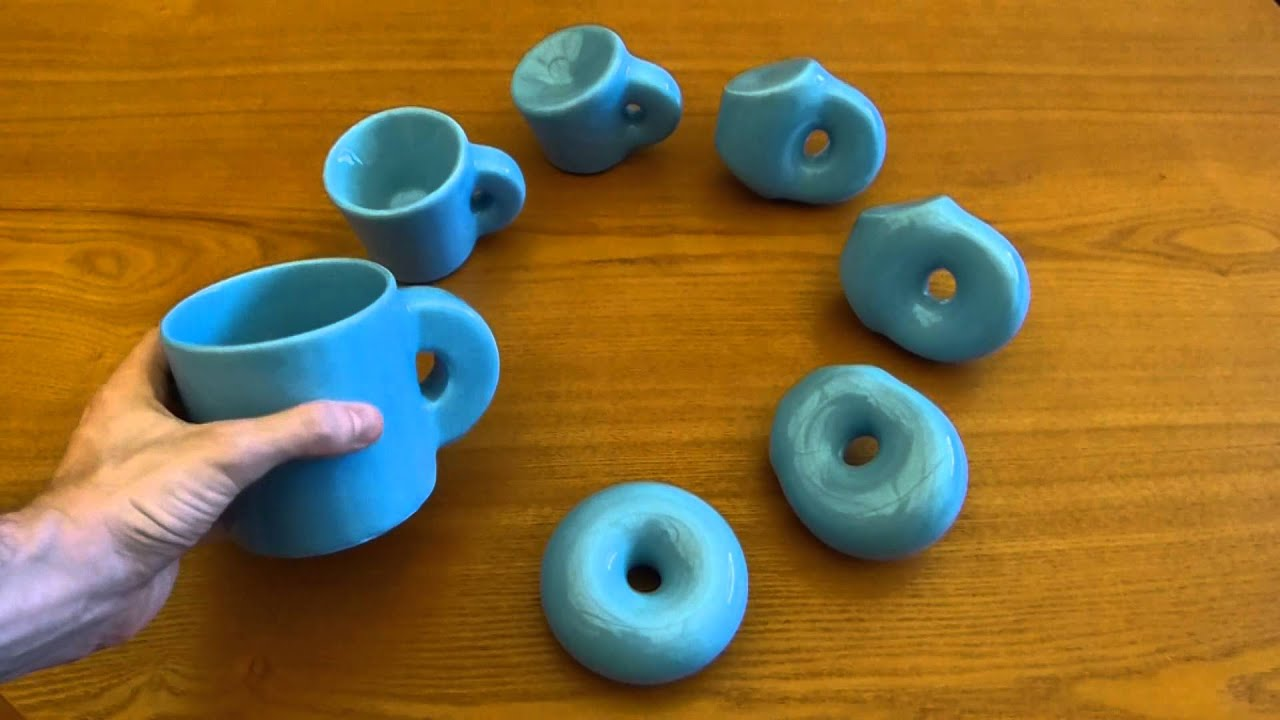
\includegraphics[width=4in]{images/topologyjoke.png}
			\caption{A classic example of a homeomorphism: A topology joke}
			\label{fig:homeomorphism}
		\end{figure}
			

	\subsubsection{Charts}
		% Charts are maps from open sets to $\R^n$
		A requirement for manifolds is that for all open sets in the manifolds, there is an attached
		chart. This chart has to be a homeomorphism from the open sets that you've declared on your set, to a subset of $\R^n$,
		which would be some union of open balls because open balls will have a standard topology.

		Suppose you have open sets $\mcal{O}_1, \mcal{O}_2$, and $\mcal{O}_3$ on a manifold $\mcal M$. If you take the union of 
		all these things that you've declared to be open, then it should become the entire manifold, from (\ref{eq:union-of-opensets}).
		Then it constitutes an open cover. For each of these sets $\mcal{O}_\alpha$, there should be a map $\psi_\alpha$ from $\mcal{O}_\alpha$ to $\R^n$.
		We can only represent these as two dimensional but these are $n$ dimensional. This is illustrated by Fig. \ref{fig:charts}

		For example, take $\mcal{O}_\alpha$, it has a chart $\psi_\alpha$ that maps it to $\R^n$. It therefore has an image $\psi_\alpha[\mcal{O}_\alpha]$ under $\psi_\alpha$
		\[
			\psi_\alpha:\mcal{O}_\alpha\to \psi_\alpha[\mcal O_\alpha]\subseteq\R^n
		\]

		\begin{figure}[h]
			\centering
			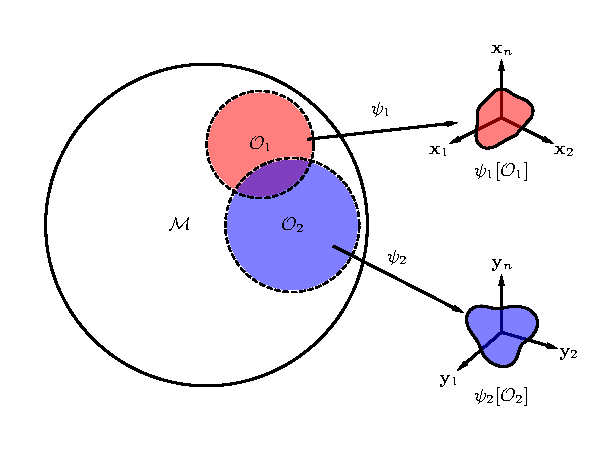
\includegraphics[width=4in,height=3in]{images/charts.pdf}
			\caption{Charts $\psi$ mapping from $\mcal{O}_\alpha$ to $\R^n$}
			\label{fig:charts}
		\end{figure}

		Now, this may sound abstract but this is something that we do in physics all the time. Because this process of providing this $\psi_1$ which
		is a map from points from $\mcal{M}$ to $\R^n$, that's nothing but a coordinate system. $\mcal M$ is just a set, an abstract set with no coordinates, it's 
		an independent object on its own, simply a collection of points constituting the elements of $\mcal M$. There is no innate coordinates
		there. When you supply it with coordinates, as we do in physics all the time, that's where the notion of manifolds comes in. 

		Manifolds are used here because we're giving each point in an abstract set $\mcal M$, say $p^i$, a set of coordinates $\vb{x}_i$. In other words we're giving a map from $\mcal O_1$ to 
		have some numerical value of each point, similar to how we assign points on the Earth (an abstract oblate-spheroidal collection of atoms and points) arbitrary longitudes and latitudes ($\R^2$).
		That is, we are \textit{charting} the manifold.
		% \[
		% 	(x^1,x^2,\ldots,x^n)\to \vb{x}_1,\vb{x}_2,\ldots,\vb{x}_n,\quad x^i\in\mcal{M},\ \vb{x}_i\in\R^n
		% \]
		\[
			\psi:\mcal O \to \R^n,\quad p\mapsto \vb{x} = (x^1(p),\ldots,x^n(p))
		\]
		Now, the requirement that $\psi_1$ needs to be a homeomorphism is a statement that $\mcal{O}_1$ and $\psi_1[\mcal{O}_1]$ are 
		topologically the same. What you did is you continuously deformed $\mcal{O}_1$ into $\psi_1[\mcal{O}_1]$, but they are topologically equivalent. There is no difference.\footnote{Jesus fucking christ all that work just to say ``we just put coordinates in objects''}
		That's all basically what it is.

		These charts are otherwise known in physics as coordinate systems. This is what I call locally $\R^n$. The coordinates that $\psi_1$ uses, only apply to $\mcal{O}_1$. If we 
		take a point outside $\mcal{O}_1$, say from $\mcal{O}_2$, then $\psi_1$ is no longer valid. It's only locally $\R^n$, because $\mcal O_2$ will have a different $\R^n$ appropriate
		to it. So that the coordinates that $\psi_1$ furnish on $\mcal O_1$ will no longer apply to any point
		that does not belong to $\mcal O_1$. The map is no longer valid.

		The final condition for a manifold to be space time is that it has to be differentiable, i.e., how the different coordinate systems
		interact with each other.

	\subsubsection{Differentiable Manifolds}
		Differentiable or smooth manifolds (both are synonymous) i.e., $C^\infty$ manifolds, are manifolds which can be differentiated
		continuously. What do we mean by that?

		Take an open set $\mcal O_1$ and $\mcal O_2$ both subsets of $\mcal M$, and overlap each other, i.e., there is a part of $\mcal O_2$ that is a subset of $\mcal O_1$ and vice versa. 
		$\psi_1$ maps $\mcal O_1$ to $\R^n$, say $\vb{x}=(x_1,x_2,\ldots,x_n)$, and $\psi_2$ maps $\mcal O_2$ to $\R^n$, say $\vb{y}=(y_1,y_2,\ldots,y_n)$. Note that these are different coordinate systems that each apply only to the chart which mapped it.
		However, since $\mcal O_1$ and $\mcal O_2$ are intersectional, then the maps must also have some parts that are intersectional. 
		That is, $\psi_1$ will map both parts of $\mcal O_1$ and $\mcal O_2$. As such, there will be a map that is $\psi_1[\mcal O_1 \cap \mcal O_2]$.
		Similarly, $\psi_2$ will map a part of $\mcal O_1$ intersectional to $\mcal O_2$, $\psi_2[\mcal O_2 \cap \mcal O_1]$.
		\begin{figure}[h]
			\centering
			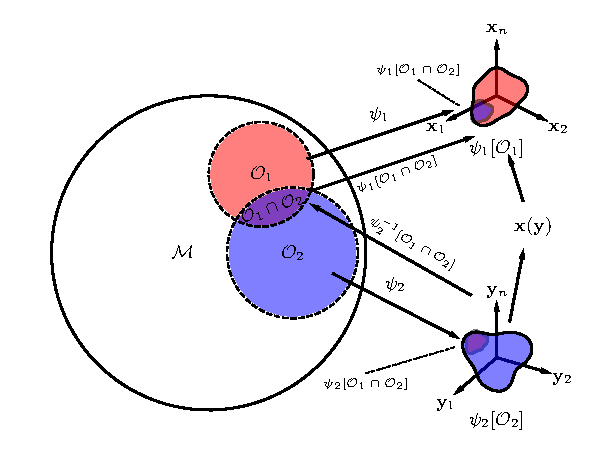
\includegraphics[width=4in,height=3in]{images/differential_manifolds.pdf}
			\caption{Differentiability of manifolds}
			\label{fig:differential-manifolds}
		\end{figure}

		Notice that you can actually map both these regions from $\psi_2[\mcal O_2 \cap \mcal O_1]$ to $\psi_1[\mcal O_1 \cap \mcal O_2]$
		directly. You can do that by constructing:
		\begin{equation}
			\label{eq:psi1psi2compose}
			\psi_1\circ \psi_2\inv : \R^n \to \R^n
		\end{equation}
		Obviously $\psi_2\inv$ only works on the region that was mapped by $\psi_2$. We can then map the preimage of $\psi_2[\mcal O_1\cap \mcal O_2]$,
		which is defined, then composing that to the map $\psi_1$ to $\R^n$, i.e., it maps from $\R^n$ to another $\R^n$, thereby bypassing the need for explicitly describing $\mcal M$. 

		Equation (\ref{eq:psi1psi2compose}) only really applies to the region $\mathcal O_1 \cap \mathcal O_2$. As such, the map $\psi_1\circ\psi_2\inv[\mcal O_1\cap\mcal O_2]$
		only really applies to $\psi_2[\mcal O_1 \cap \mcal O_2]$, not to all of $\R^n$.
		\[
			\psi_1 \circ \psi_2^{-1} : 
			\underbrace{\psi_2[\mathcal{O}_1 \cap \mathcal{O}_2]}_{\subseteq \mathbb{R}^n} 
			\to 
			\underbrace{\psi_1[\mathcal{O}_1 \cap \mathcal{O}_2]}_{\subseteq \mathbb{R}^n} 
		\]
		\newpage
		This can be written in the more concrete usual notation as $\vb{x}$ being a function of $\vb{y}$, i.e., taking the $\vb y$ coordinates and spitting out the $\vb x$ coordinates:
		\begin{equation}
			\label{eq:differentialmanifolds-RntoRN}
			\psi_1\circ \psi_2\inv \iff \vb{x}(\vb{y})
		\end{equation}
		These are called \textbf{transition functions} in the math literature. But for now, we'll call it, simply, as coordinate transformations. 

		Now, let's go back to the definition of a manifold, Def. 3.3, we see that \textit{all such transition functions} $\psi_\beta\circ\psi_\alpha\inv$ \textit{must be }$C^\infty$.

		This is the last key part, and we have now explained all the terms needed to define a differentiable manifold (a.k.a., $C^\infty$ manifolds). The definition of a $C^\infty$ manifold
		requires that all such coordinate transformations are $C^\infty$, and we understand $C^\infty$ in the usual sense, because in normal calculus, you can take as many 
		derivatives as you want, and still be continuous. This is applicable because $\vb{x}(\vb y)$ is a usual $\R^n\to \R^n$ function, it is something that everybody understands.
		All objects like these should be infinitely differentiable. One should take as many derivatives as they want.

		So again, what is a manifold? It's simply a set of open sets with coordinate systems, and every time the open sets overlap, the transition functions (coordinate transformations) must
		always be infinitely differentiable, if it is to be a $C^\infty$ manifold.
		\begin{question}{About the notion of $C^\infty$, if you take derivatives again and again of a function, wouldn't it at some point become zero? And so, it seems impossible for it to be infinitely differentiable.}
			It is still differentiable! If you can differentiate a zero function, it is still differentiable, and the result is 0 again, \textit{ad infinitum}, you can still keep on going, and the result remains continuous. 
			What we mean by differentiability here is the usual criteria for differentiability which are the lack of spikes or discontinuities that will make the manifold undifferentiable at that point. We require these to be \textit{smooth}.
			When we get to black holes, we will find that the coordinate systems will break down precisely when you encounter violations of this requirement to be infinitely differentiable,
			which signifies we reached the end of our chart, and we need a new coordinate system. 
		\end{question}	
		One of the things which you should sort of take from this notion of a manifold is that the coordinate 
		systems can lead you astray. The manifolds can be very well defined and well behaved. However, at some point, the transformation will cause a divergence which is not allowed by your
		chosen coordinate transformation, that will signify you have a problem with the chart, it has gone beyond where it can represent, by which you need to find another coordinate transformation which fits your uses.
		There are other kinds of manifolds which are not $C^\infty$, mathematicians may sometimes demand only $C^2$. So sometimes you may 
		see people say $C^2$ manifold, because for the transition functions, they only want it to be 
		$C^2$. Sometimes they say topological manifold, this is simply a $C^0$ manifold, it is only continuous but the derivatives are not. 
		For us in physics, we're always going to use infinitely differentiable manifolds. If we see a manifold, we will always demand for it to be a $C^\infty$, or a smooth, or differentiable manifold.
		This is what we demand of spacetime.


		The entire set of open-set/chart pairs, since it is an open cover, is called an atlas (to continue the analogy with maps)
		\[
			\text{Atlas} \equiv \qty{(\psi_\alpha,\mathcal O_\alpha)}
		\]
		The unions of $\mcal O_\alpha$ and $\psi_\alpha$ constitute an atlas on $S^2$

		% That's the last bit of terminology, before we have understood all the terms that were said in the definitions for space time, and for a manifold.
	\subsubsection{Examples}
		\begin{enumerate}[(1)]
			\item $\R^n$
				
				Obviously. $\R^n$ itself is a manifold. In fact, the nice thing about $\R^n$ is that it can be covered by a single chart. For $\R^n$, it's just the usual $\R^n$.
				This chart is that the identity transformation:
				\[
					\text{Id}: \R^n \to\R^n
				\]
			\item $S^2$

				$S^2$, the two sphere, has various ways to coordinatize. One way is by the so-called stereographic projection (Fig. \ref{fig:stereographicprojection}).
				We want a chart $\psi$ that globally maps all of $S^2$ to $R^2$, such that $\psi:S^2\to\R^2$. One nice map is called the stereographic projection, where we coordinatize 
				points by using the north pole $N$, and projecting a line from $N$ to any point in $S^2$, $p$ until it intersects a plane described by $\R^2$. 
				We can place the plane to be coincident with the center of $S^2$ or on the south pole $S$. The intersection point on the plane, $(x,y)$ is then the map from the surface of $S^2$ to $\R^2$.
				\[
					\psi_N:p\mapsto(x,y)
				\]
				This is simply a way of assigning $S^2$ to $\R^2$. However, since we map $S^2$ from  the point $N$, it cannot be 
				projected onto the plane, hence, it is not represented in $\R^2$
				\[
					\psi_N: S^2-\{N\} \to \R^2
				\]
				This is an example of a coordinate system which can have multiple charts. $\psi_N$ is insufficient to describe all of 
				$S^2$, hence, we need another map. We will construct the same projection, where we attach the plane to be coincident with $N$, 
				and instead take the line from $S$ to project to the plane. This is now
				\[
					\psi_S = S^2 - \{S\} \to \R^n 
				\]
				We call $S^2 - \{S\}=\mcal O_S$ and $S^2 - \{N\}=\mcal O_N$. Note that the union is the entire manifold.
				\[
					\mcal O_N \cup \mcal O_S = S^2
				\]
				So, $\qty{\psi_N,\mcal O_N}$ and $\qty{\psi_S,\mcal O_S}$ constitute an atlas for $S^2$.

				Another way is to use longitude and colatitude, the usual way to coordinatize a sphere
				\[
					(\theta,\phi)
				\]
				where $\theta$ is the colatitude, $\theta=[0,\pi]$, and $\phi$ is the longitude, ($\phi = [0, 2\pi)$). 
				With this method, we can also embed $S^2$ to $\R^3$. This chart maps all of $S^2$ to a \textit{subset}
				of $\R^2$. However, it has two main problems: (1) At the poles, longitude is undefined, for every longitude line
				meets there, therefore $\phi$ is undefined, and the system breaks down, and (2) The longitude wraps around, with $0$ and $2\pi$ representing
				the same meridian, so the mapping repeats.

				However, it is a very useful coordinate system on most of the sphere, but not a global chart. In that sense, other maps
				are needed to complete the entire atlas. 
				This illustrates why a manifold may require multiple coordinate charts to describe it globally. For most intents and purposes,
				using the latitude-longitude convention is very useful. However, due to it's limitations in describing all points on $S^2$,
				other projection mappings are preferred.

				These are just two ways to
				map $S^2$, there are other ways to do so which are more contrived, but I encourage you to study them
		\end{enumerate}

		\begin{figure}[h]
			\centering
			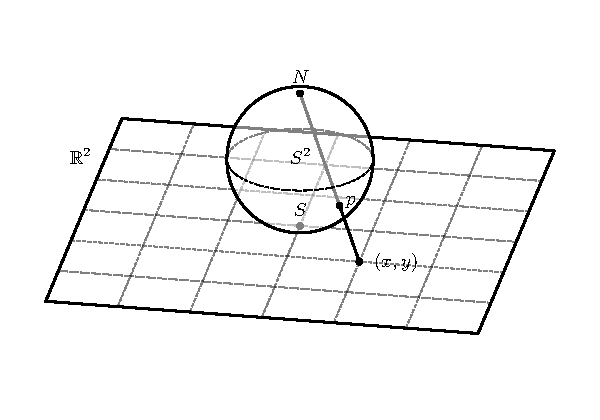
\includegraphics[width=4in, height=2.8in]{images/sterographicprojection.pdf}
			\caption{Stereographic projection of $S^2$ to $\R^2$, using $N$}
			\label{fig:stereographicprojection}
		\end{figure}
	
		Like we said in the beginning, literally anything in physics where we use coordinates is a manifold. Normally in most areas of physics, we're not too careful
		about the manifold because we mostly think about the stuff on top of the manifold. However, this is spacetime physics,
		when we study spacetime, spacetime itself \textit{is} the manifold. So we have to consider the manifold itself. Anything you might conceive of, field theory (fields living in $\R^4$, coordinatized by $t$ and $\vb x$),
		mechanics (which lives in phase space, coordinatized by $x$ and $p$), thermodynamics, which are also manifolds coordinatized by thermodynamic variables. Literally anything 
		where you're using coordinates, there is an underlying manifold there. 

		Very roughly, we wouldn't be too far off from the definition that basically a manifold is something that it's a set and that it's locally coordinatizable, and 
		that locally is equivalent to $\R^n$. If you can put coordinates on a set, you essentially have a manifold.

		Now, obviously the question would be: What are not manifolds? They do exist, those are the sets which does not have
		the things we demand of them. For example, A geometric object that appears to self-intersect in an embedding may fail to be a manifold at the intersection point, 
		for the definitiones required will fail at the interseciton.

		In physics, GR especially, we respect the democracy of coordinate systems. Charts are just there as computational devices.
		They have to interact with charts in such a way that we get coodinate transformations, infinitely continuous. If your transformation
		is not continuously differentiable, which means you have a divergence somewhere, it means that your chart is invalid. It signals that 
		the domain of your chart is probably smaller than you imagined.
			
	\paragraph{Addendum}
		A pretty neat description of a topological manifold I found from Robbin and Salamon, which is at least clear for me, goes as follows:
		\begin{definition}{Topological Manifold}
			A topological manifold is a topological space $\mcal M$ such
			that each point $p\in M$ has an open neighborhood $\mcal O$ which is homeomorphic
			to an open subset of a Euclidean space.	    
		\end{definition}
		This is far more succint than the definition presented in the lecture.
		

				
			

		


			



		
		

		
		
		
		


		\newpage
		% =============================================
% MEETING 5
% ---------------------------------------------
% DATE   - SEPTEMBER 2, 2026
% FORMAT - FACE TO FACE
% =============================================
% TOPIC  - STRUCTURES ON MANIFOLDS
% =============================================

\subsection{Structures on Manifolds}

	We begin this meeting by recapping what we learned from the previous
	lecture, namely differentiable manifolds, charts, and topology. We then
	develop the notion of spacetime as a differentiable manifold and discuss
	the importance of describing the laws of physics in terms of geometric 
	objects rather than particular coordinate systems. From there, we introduce
	scalar fields and, more importantly, develop the definition of vectors on a
	general manifold through the idea of directional derivatives. 

	\subsubsection{Spacetime as a Manifold}
		We consider spacetime to be a differentiable, or smooth, manifold.
		That is, spacetime is a topological space which is \textit{locally}
		homeomorphic to $\R^n$, together with additional structure that allows
		us to perform calculus.

		The important point is that a manifold does not, in general, possess
		a single global coordinate system. Instead, we describe it using
		coordinate patches, or \textit{charts}, each of which maps a portion
		of the manifold into $\R^n$.

		For example, consider a three-dimensional manifold $\mcal{M}$.
		Suppose that $Q_1,Q_2\subset\mcal{M}$ are two overlapping coordinate
		patches. On $Q_1$, we may introduce spherical coordinates
		\[
			\vb{r}=(r,\theta,\phi),
		\]
		while on $Q_2$ we may introduce Cartesian coordinates
		\[
			\vb{x}=(x,y,z).
		\]
		A chart is a pair
		\[
			\qty{Q_\alpha,\psi_\alpha},
		\]
		where $\psi_\alpha$ is a map from the manifold to $\R^n$. It is a coodinate system, so to speak.
		\[
			\psi_\alpha:Q_\alpha\to\R^n
		\]
		maps points on the manifold to their coordinate representations.

		Thus, if $p\in Q_1\cap Q_2$, we can describe the same point using
		either coordinate system:
		\[
			\psi_1(p)=\vb{r},
			\qquad
			\psi_2(p)=\vb{x}.
		\]

		Since the two charts overlap, we can move from one coordinate
		representation to the other by composing one chart with the inverse
		of the other:
		\begin{equation}
			\vb{x}
			=
			\psi_2\circ\psi_1^{-1}(\vb{r}).
		\label{eq:coordinate-transition-x-from-r}
		\end{equation}
		Likewise,
		\begin{equation}
			\vb{r}
			=
			\psi_1\circ\psi_2^{-1}(\vb{x}).
		\label{eq:coordinate-transition-r-from-x}
		\end{equation}
		More directly, we can represent $\vb{x}$ as a function of $\vb{r}$, and 
		vice versa.
		\[
			\vb{x}(\vb r)
			\quad
			\longleftrightarrow
			\quad
			\vb{r}(\vb x)
		\]

		The maps
		\[
			\psi_\beta\circ\psi_\alpha^{-1}
		\]
		are called \textit{transition maps}. The requirement that these
		transition maps be sufficiently differentiable is what allows the
		manifold to be given a differentiable structure.
		\begin{figure}[h]
			\centering
			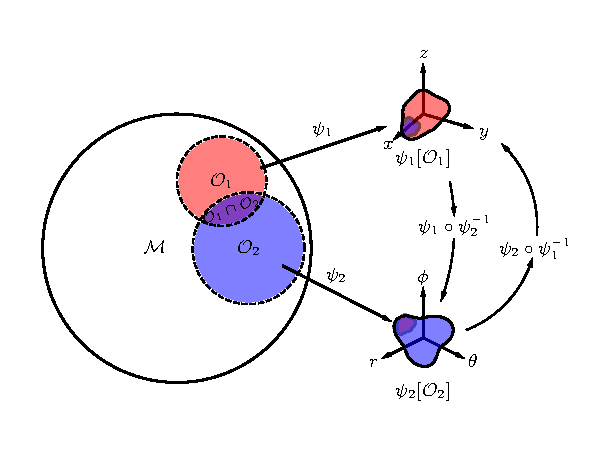
\includegraphics[width=4in, height=3in]{images/manifold_example.pdf}
			\caption{An example of a manifold being represented in different
			coordinate systems, cartesian and polar in this case, and how to interchange between them using transition functions.}
			\label{fig:manifold-coordinate-systems}
		\end{figure}

		A collection of charts whose domains cover the manifold,
		\[
			\mcal{M}=\bigcup_\alpha Q_\alpha,
		\]
		is called an \textit{atlas}. The charts are required to be compatible
		on their overlaps:
		\begin{equation}
			\psi_\beta\circ\psi_\alpha^{-1}
			:
			\psi_\alpha(Q_\alpha\cap Q_\beta)
			\to
			\psi_\beta(Q_\alpha\cap Q_\beta)
			\label{eq:transition-map}
		\end{equation}
		must be smooth wherever the two coordinate patches overlap.

		This is the essential idea behind a differentiable manifold. We do
		not require the manifold itself to resemble $\R^n$ globally. We only
		require that, in sufficiently small neighborhoods, it can be
		described using ordinary Euclidean coordinates.

		The existence of multiple charts is particularly useful when a
		coordinate system develops a \textit{coordinate singularity}. If one
		coordinate system becomes inconvenient or singular in some region,
		we may simply use another chart which covers that region and the singularity
		does not exist.

		For example, spherical coordinates are singular at $r=0$ and at the
		poles where $\theta=0,\pi$. These singularities need not represent
		anything physically pathological; they may simply indicate that the
		chosen coordinates have broken down.

		In general relativity, this distinction is crucial. A coordinate
		singularity is not necessarily a physical singularity, it may only be 
		a mathematical artifact. For example,
		the Schwarzschild coordinates possess a coordinate singularity at
		$r=2GM$ (in units where $c=1$), which can be removed by changing
		coordinates. By contrast, the Schwarzschild curvature singularity
		at $r=0$ is a genuine physical singularity and is not removed by a
		mere change of coordinates.

	\subsubsection{General Covariance}

		The central lesson of the manifold formulation is that the laws of
		physics should not depend on the particular coordinate system used
		to describe them, this is known as general covariance. As long as the coordinate system is appropriate, one
		may use any system he or she desires that makes the physics being
		performed more convenient, as long as the limits of such formulation is known.
		In general relativity, physical quantities should therefore be
		expressed in terms of geometric objects which possess well-defined
		transformation properties under changes of coordinates.

		Among the objects we will encounter are:
		\begin{enumerate}[(a)]
		\item scalars,
		\item vectors,
		\item one-forms, or dual vectors,
		\item tensors,
		\item spinors.
		\end{enumerate}

		Spinors require some additional structure beyond the ordinary tensor
		bundle and therefore do not fit directly into the elementary tensor
		description of general relativity. Nevertheless, spinor fields can
		be defined on suitable spacetime manifolds and are important when
		describing fermionic matter.

		The purpose of this meeting is to construct these geometric objects
		starting from the manifold itself.

	\subsubsection{Scalar Functions}

		A scalar field is the simplest geometric object that we can define
		on a manifold. It is simply a function which assigns one real number
		to every point of the manifold:
		\begin{equation}
			f:\mcal{M}\to\R.
			\label{eq:scalar-function}
		\end{equation}
		There is no coordinate system involved in the definition itself.

		Given a point $p$ in the manifold.
		\[
			p\in\mcal{M},
		\]
		the scalar field simply assigns $p$ to a real number
		\[
			f: p\mapsto f(p)\in\R.
		\]

		Coordinates only enter when we wish to represent the scalar field
		explicitly. Given a chart
		\[
			\psi:Q\subset\mcal{M}\to\R^n,
		\]
		we can construct the coordinate representation of $f$ by composing
		it with the inverse chart:
		\begin{equation}
			f\circ\psi^{-1}:\R^n\to\R.
			\label{eq:scalar-coordinate-representation}
		\end{equation}

		Writing
		\[
			\vb{x}  = \psi(p)
			=
			\qty(x^1,x^2,\ldots,x^n),
		\]
		we therefore obtain the familiar expression of a scalar field.
		\begin{equation}
			f:\vb{x}
			\mapsto
			f\circ\psi^{-1}(\vb{x})
			\equiv
			f(\vb{x}).
			\label{eq:scalar-chart-representation}
		\end{equation}

		\begin{figure}[h]
			\centering
			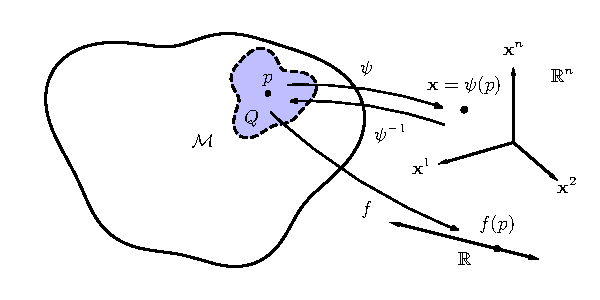
\includegraphics[width=4in, height=2in]{images/manifoldtoscalar.pdf}
			\caption{A scalar function as a map from a manifold to the real
			numbers.}
			\label{fig:manifold-to-scalar}
		\end{figure}

		The coordinate representation of the function arises
		only after choosing a chart.
		Thus, the coordinates
		\[
			\vb{x}\equiv(x^1,x^2,\ldots,x^n)
		\]
		should not be confused with points of the manifold themselves.
		They are merely the coordinate representation of points in a
		particular chart.
		The manifold itself is coordinate-independent.

		To perform differential geometry, we require our functions to possess
		the appropriate degree of differentiability. A function is called
		\textit{smooth} if its coordinate representation is infinitely
		differentiable:
		\begin{equation}
			f\in C^\infty(\mcal{M}).
			\label{eq:smooth-function}
		\end{equation}

		We may denote the set of all smooth real-valued functions on
		$\mcal{M}$ by
		\begin{equation}
			\mcal{F}(\mcal{M})
			\equiv
			C^\infty(\mcal{M}).
			\label{eq:smooth-function-space}
		\end{equation}

		An important example of scalar functions are the coordinate
		functions themselves. Given a chart $\psi$, we may write
		\begin{equation}
			x^\alpha(p)
			\equiv
			\psi^\alpha(p),
			\label{eq:coordinate-function}
		\end{equation}
		where $\psi^\alpha$ denotes the $\alpha$th component of the chart.

		Thus, each coordinate $x^\alpha$
		is itself a scalar function on the region covered by the chart.
		This point will become important when we construct vectors.

	\subsubsection{Vectors}
		The concept of a vector space is undoubtedly familiar to most readers. 
		In prerelativity physics it is assumed that space has the natural structure of a three
		dimensional vector space once one has designated a point to serve as the origin; the
		natural rules for adding and scalar multiplying spatial displacements satisfy the
		vector space axioms. In special relativity, spacetime similarly has the natural structure 
		of a four-dimensional vector space. 

		However, when one considers curved
		geometries (as we do in general relativity), this vector space structure is lost. For
		example, there is no natural notion of how to \textit{add} two points on a sphere and end
		up with a third point on the sphere. Nevertheless, vector space structure can be
		recovered in the limit of "infinitesimal displacements" about a point. It is this notion
		of "infinitesimal displacements" or tangent vectors which lies at the foundation of
		calculus on manifolds. Therefore, we will devote considerable attention below to
		giving a precise mathematical definition of this concept.

		The ordinary notion of a vector comes from linear algebra.

		A vector is an algebraic object that belongs to a vector space $\bb{V}$, which is an algebraic
		structure equipped with operations of vector addition and scalar
		multiplication satisfying the usual vector-space axioms, which defines what multiplication and 
		addition is, and what is a unit and a zero vector, among other things. However, in this case, we 
		are concerned about closure and linearity.

		In particular, if
		\[
		    \vb{v}_1,\vb{v}_2\in\bb{V},
		    \qquad
		    \alpha,\beta\in\R,
		\]
		then closure requires
		\begin{equation}
			\alpha\vb{v}_1+\beta\vb{v}_2\in\bb{V}.
			\label{eq:vector-space-closure}
		\end{equation}

		Anything can be called a vector provided that it satisfies all the
		axioms defining a vector space. There is therefore no requirement
		that a vector must necessarily be represented as an arrow in
		Euclidean space.

		The familiar arrow picture is a useful visualization, but it is not
		the fundamental definition of a vector.

		In $\R^3$, we normally introduce vectors as directed line segments.
		Given points $p$ and $q$, for example, one can draw an arrow pointing
		from $p$ to $q$.

		\begin{figure}[h]
			\centering
			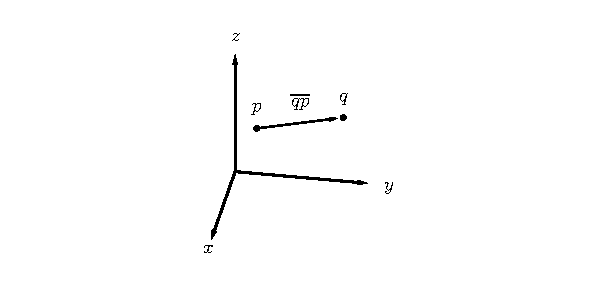
\includegraphics[width=4in,height=2in]{images/R3vectors.pdf}
			\caption{The familiar representation of vectors as directed
			arrows in Euclidean space. This picture relies on the affine
			structure of $\R^3$.}
			\label{fig:R3-vectors}
		\end{figure}

		There is, however, a subtlety here.

		In Euclidean space, we possess an \textit{affine structure}: points
		can be subtracted to obtain vectors, and vectors can be added to
		points. Thus, if $p$ and $q$ are points in $\R^3$, the displacement
		\[
			q-p \equiv \overline{qp}
		\]
		is naturally interpreted as a vector.  

		A general manifold does not possess this structure. It is not applicable or intrinsic to the manifold itself. In particular,
		there is no natural operation $q-p$
		for two arbitrary points $p,q\in\mcal{M}$.

		Therefore, if we want to define vectors on a general manifold, we
		need a definition which does not depend upon arrows, position
		vectors, or the ability to subtract points.

		The solution is to define vectors in terms of \textit{directional
		derivatives}.

	\subsubsection{Directional Derivatives}

		In $\R^n$, suppose that $\vb{v}_p$ is a vector based at the point
		$p$. Given a smooth function $f$, its directional derivative in the
		direction $\vb{v}_p$ is
		\begin{equation}
			\vb{v}_p(f)
			\equiv
			\lim_{t\to0}
			\frac{
			f(\vb{x}_p+t\vb{v}_p)-f(\vb{x}_p)
			}{t}.
			\label{eq:directional-derivative}
		\end{equation}

		In ordinary vector calculus, this is equivalent to
		\begin{equation}
			\vb{v}_p(f)
			=
			\vb{v}_p\cdot\grad f(p)
			\label{eq:directional-derivative-gradient}
		\end{equation}

		However, Eq. (\ref{eq:directional-derivative}) makes use of the
		affine structure of $\R^n$, since it explicitly contains
		\[
			\vb{x}_p+t\vb{v}_p.
		\]
		We therefore seek a definition which retains the algebraic properties
		of a directional derivative without requiring us to add vectors to
		points.

		The key observation is that the directional derivative is an
		\textit{operator acting on functions}.

		Consider a vector $\vb{v}_p$ acting on two smooth functions $f$ and
		$g$. Directional differentiation satisfies two fundamental
		properties.
		\begin{enumerate}[(1)]
			\item It is linear:
				\begin{equation}
					\vb{v}_p(\alpha f+\beta g)
					=
					\alpha\vb{v}_p(f)
					+
					\beta\vb{v}_p(g),
					\label{eq:vector-linearity}
				\end{equation}
				for
				\[
					\alpha,\beta\in\R,\qquad f,g\in\mcal{F}(\R^n)
				\]
			\item It satisfies the Leibniz rule:
				\begin{equation}
					\vb{v}_p(fg)
					=
					f(p)\vb{v}_p(g)
					+
					g(p)\vb{v}_p(f).
					\label{eq:vector-leibniz}
				\end{equation}
		\end{enumerate}
		These two properties do not require an affine structure.

		We therefore take them as the fundamental definition of a tangent
		vector.

		\begin{definition}{Tangent Vector}
			A tangent vector at $p\in\mcal{M}$ is a linear map of manifolds to real functions 
			\begin{equation}
				\vb{v}_p:
				\mcal{F}(\mcal{M})\to\R^n
				\label{eq:tangent-vector-definition}
				\end{equation}
				which satisfies the Leibniz rule
				\begin{equation}
				\vb{v}_p(fg)
				=
				f(p)\vb{v}_p(g)
				+
				g(p)\vb{v}_p(f).
				\label{eq:tangent-vector-leibniz}
			\end{equation}
		\end{definition}

		Thus, we define vector is nothing but a derivative operator on a manifold satisfying the
		appropriate algebraic properties.


		This also explains why the usual arrow does not appear in the
		definition.
		The arrow is only our preconceived geometric picture of a vector.
		The fundamental object is the action of the vector on functions.
		\begin{figure}[h]
			\centering
			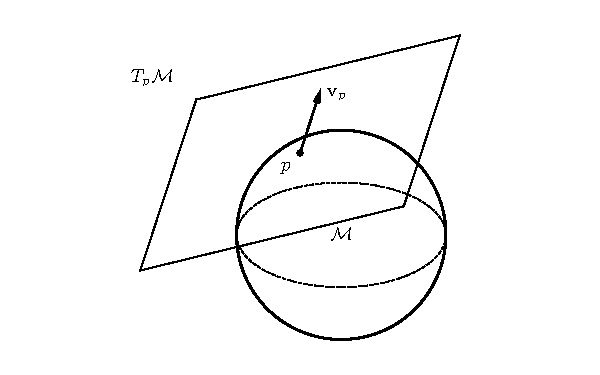
\includegraphics[width=4in, height = 2.5in]{images/vectordef.pdf}
			\caption{A tangent vector $\vb{v}$, represented as a directional derivative
			lying in the tangent plane at a point $p$ of the manifold, in this case, a surface embedded on a sphere in $\R^3$. The tangent plane in this
			case represents the tangent space $T_p \mcal{M}$}.
			\label{fig:vector-definition}
		\end{figure}


	\subsubsection{The Tangent Space}

		The collection of all tangent vectors at a point $p$ forms a vector
		space.

		\begin{theorem}{Tangent Space}
			The set of all tangent vectors at $p\in\mcal{M}$ forms a vector
			space, called the \textit{tangent space at $p$}, denoted
			\begin{equation}
				T_p\mcal{M}.
				\label{eq:tangent-space}
			\end{equation}
		\end{theorem}

		\begin{proof}
			Let $\vb{v}_p,\vb{w}_p\in T_p\mcal{M}$.

			We define vector addition by the plus operator, $+$. It acts likeso
			\begin{equation}
				(\vb{v}_p+\vb{w}_p)(f)
				\equiv
				\vb{v}_p(f)+\vb{w}_p(f),
				\label{eq:tangent-vector-addition}
			\end{equation}
			and scalar multiplication by the following operation:
			\begin{equation}
				(\alpha\vb{v}_p)(f)
				\equiv
				\alpha\vb{v}_p(f).
				\label{eq:tangent-vector-scalar-multiplication}
			\end{equation}

			The zero vector is defined by
			\begin{equation}
				\vb{0}_p(f)=0.
				\label{eq:tangent-zero-vector}
			\end{equation}

			We must verify closure. For the sum,
			\begin{align}
				(\vb{v}_p+\vb{w}_p)(fg)
				&=
				\vb{v}_p(fg)+\vb{w}_p(fg)
				\nonumber\\
				&=
				f(p)\vb{v}_p(g)
				+g(p)\vb{v}_p(f)
				\nonumber\\
				&\quad
				+f(p)\vb{w}_p(g)
				+g(p)\vb{w}_p(f)
				\nonumber\\
				&=
				f(p)(\vb{v}_p+\vb{w}_p)(g)
				+
				g(p)(\vb{v}_p+\vb{w}_p)(f).
				\label{eq:tangent-space-closure}
			\end{align}

			Hence $\vb{v}_p+\vb{w}_p$ also satisfies the Leibniz rule and is
			therefore a tangent vector.

			Similarly, for $\alpha\in\R$,
			\begin{align}
				(\alpha\vb{v}_p)(fg)
				&=
				\alpha\vb{v}_p(fg)
				\nonumber\\
				&=
				\alpha f(p)\vb{v}_p(g)
				+
				\alpha g(p)\vb{v}_p(f)
				\nonumber\\
				&=
				f(p)(\alpha\vb{v}_p)(g)
				+
				g(p)(\alpha\vb{v}_p)(f).
				\label{eq:tangent-space-scalar-closure}
			\end{align}

			Therefore the set of tangent vectors satisfies closure under
			addition and scalar multiplication, and the remaining vector
			space axioms follow from the corresponding properties of the
			real numbers.
		\end{proof}

		From these, we also prove that the corollary expressions are also linear.
		\[
			(\alpha \vb{v}_p + \beta \vb{w}_p) (f) = \alpha \vb{v}_p (f) + \beta \vb{w}_p (f)
		\]
		and
		\[
			(\alpha \vb{v}_p + \beta \vb{w}_p)\cdot\grad f
			=
			\alpha \vb{v}_p \cdot \grad f + \beta \vb{w}_p \cdot \grad f
		\]
		Every vector in $T_p\mcal{M}$ is therefore associated with the same
		point $p$. This is different from the elementary picture of vectors
		in $\R^n$, where vectors are often drawn with their tails at the
		origin.

		A tangent vector does not have to be thought of as an arrow extending
		from one point of the manifold to another. It belongs to the tangent
		space \textit{at a particular point}.

	\subsubsection{The Coordinate Basis}
		We now construct an explicit basis for $T_p\mcal{M}$.

		Suppose that
		\[
		    \qty{Q,\psi}
		\]
		is a chart around $p$, with coordinates
		\[
		    \qty{x^1,x^2,\ldots,x^n}.
		\]
		We define the coordinate basis vectors by their action on a smooth
		function $f$:
		\begin{equation}
			(\partial_\mu)_p(f)
			\equiv
			\eval{
			\pdv{(f\circ\psi^{-1})}{x^\mu}
			}_{\psi(p)}.
			\label{eq:coordinate-basis-definition}
		\end{equation}

		The notation
		\[
		    (\partial_\mu)_p
		\]
		should therefore be interpreted as a map acting on functions.

		In other words,
		\[
		    (\partial_\mu)_p
		    :
		    \mcal{F}(\mcal{M})\to\R.
		\]
		The derivative is taken not directly on the abstract manifold, but
		on the coordinate representation
		$f\circ\psi\inv$ in $\R^n$.

		The remarkable fact is that these coordinate derivative operators
		form a basis for the entire tangent space.

		\begin{theorem}{Coordinate Basis of the Tangent Space}
			Given a chart $\qty{Q,\psi}$ with coordinates
			$\qty{x^1,\ldots,x^n}$, the set
			\begin{equation}
			\qty{
			(\partial_1)_p,
			(\partial_2)_p,
			\ldots,
			(\partial_n)_p
			}
			\label{eq:coordinate-basis-set}
		\end{equation}
		constitutes a basis for $T_p\mcal{M}$.
		\end{theorem}

		\begin{proof}
			We prove linear independence and spanning separately.
			\begin{enumerate}[(1)]
				\item Linear Independence
					
					Recall that vectors $\vb{v}_1, \vb{v}_2,\ldots,\vb{v}_n$ are linearly 
					independent if 
					\[
						\alpha^1 \vb{v}_1 + \alpha^2 \vb{v}_2 + \cdots + \alpha^n \vb{v}_n = \vb{0} \qquad\equiv a^\mu(\p_\mu) = \vb{0}
					\]
					implies that
					\[
						\alpha^1=\alpha^2=\cdots=\alpha^n = 0 \qquad \equiv a^\mu = 0
					\]
					In this case, we shall prove that is indeed the case. 

					Suppose that some coefficients $\alpha^\mu$ and the basis sums to zero.
					\begin{equation}
						\alpha^\mu(\partial_\mu)_p
						=
						\vb{0}_p
						\label{eq:basis-linear-independence-assumption}
					\end{equation}

					Acting on an arbitrary function $f$ gives
					\begin{equation}
						\alpha^\mu(\partial_\mu)_p(f)
						=
						0.
						\label{eq:basis-linear-independence-action}
					\end{equation}

					In particular, since it is convenient, we choose $f=x^\nu$. Then
					\begin{equation}
						\alpha^\mu(\partial_\mu)_p(x^\nu)=0.
						\label{eq:basis-linear-independence-coordinate}
					\end{equation}

					By definition,
					\begin{align}
						(\partial_\mu)_p(x^\nu)
						&=
						\eval{
							\pdv{
								(x^\nu\circ\psi^{-1})
							}{x^\mu}
						}_{\psi(p)}
						\nonumber\\
						&=
						\eval{
							\pdv{x^\nu}{x^\mu}
						}_{p}
						\nonumber\\
						&=
						\tensor{\delta}{^\nu_\mu}
						\label{eq:coordinate-basis-delta}
					\end{align}

					Hence,
					\begin{align}
						\alpha^\mu\tensor{\delta}{^\nu_\mu}
						&=
						\alpha^\nu\\
						\nonumber
						&=
						0
						\label{eq:basis-alpha-zero}
					\end{align}

					Therefore the coordinate basis vectors are linearly independent.

				\item Spanning\footnote{Wald, p.16}

					Let
					\[
						\vb{v}_p\in T_p\mcal{M}.
					\]

					Define the components of $\vb{v}_p$ with respect to the
					coordinate basis as the action of the operator on that basis.
					\begin{equation}
						v^\nu
						\equiv
						\vb{v}_p(x^\nu).
						\label{eq:vector-components}
					\end{equation}

					We claim that
					\begin{equation}
						\vb{v}_p
						=
						v^\mu(\partial_\mu)_p.
						\label{eq:vector-basis-expansion}
					\end{equation}

					To see this, let $f$ be an arbitrary smooth function. The
					coordinate representation of $f$ is a smooth function of
					$x^1,\ldots,x^n$, so its ordinary multivariable differential
					gives
					\begin{equation}
						\vb{v}_p(f)
						=
						v^\mu(\partial_\mu)_p(f).
						\label{eq:vector-acting-on-function}
					\end{equation}

					Since the two tangent vectors have the same action on every
					smooth function, they are the same vector. Hence
					\[
						\vb{v}_p
						=
						v^\mu(\partial_\mu)_p.
					\]
					Therefore the coordinate vectors span $T_p\mcal{M}$.
			\end{enumerate}
			That completes the proof.
		\end{proof}

		Thus every tangent vector can be written in the form
		\begin{equation}
			\vb{v}_p
			=
			v^\mu(\partial_\mu)_p.
			\label{eq:vector-coordinate-expansion}
		\end{equation}

		Suppressing the explicit point label when there is no ambiguity,
		we conventionally write
		\begin{equation}
			\vb{v}
			=
			v^\mu\partial_\mu.
			\label{eq:abstract-vector-expansion}
		\end{equation}

		This is the origin of the familiar ``arrow'' notation in a traditional coordinate
		basis, $\vb{v} = v^\mu \vb{e}_\mu$. In this case, we prove that the coordinate
		basis is therefore similar, but not exactly equivalent to the elementary basis vectors. 
		We shall expound more on this next meeting.
		\[
			\vb{e}_\mu \equiv \partial_\mu = \eval{\pdv{}{x^\mu}}_{p}
		\]

		For example, in Cartesian coordinates on $\R^3$,
		\begin{equation}
			\vb{v}
			=
			v^x\pdv{}{x}
			+
			v^y\pdv{}{y}
			+
			v^z\pdv{}{z}.
			\label{eq:cartesian-vector}
		\end{equation}

		In spherical coordinates, the very same tangent vector can instead
		be represented as
		\begin{equation}
			\vb{v}
			=
			v^r\pdv{}{r}
			+
			v^\theta\pdv{}{\theta}
			+
			v^\phi\pdv{}{\phi}.
			\label{eq:spherical-vector}
		\end{equation}

		The components
		$
		    v^\mu
		$
		change when we change coordinates, while the geometric vector
		$\vb{v}$ itself does not.

		This is one of the central ideas of differential geometry:

		\begin{quote}
			The vector is the geometric object; its components are merely its
			representation in a chosen basis.
		\end{quote}

	\subsubsection{Abstract Index Notation (Preliminary)}

		In general relativity, it is useful to distinguish between a vector
		as an abstract geometric object and its components in a particular
		coordinate system.

		We may therefore write
		\[
			\vb{v}
		\]
		for the vector itself, while
		\[
			v^\mu
		\]
		denotes its components with respect to the coordinate basis
		$\partial_\mu$.

		Thus,
		\begin{equation}
			\vb{v}
			=
			v^\mu\partial_\mu
			\label{eq:abstract-index-vector}
		\end{equation}

		The index $\mu$ is not itself a coordinate label such as $x$ or $y$.
		It is an abstract index indicating which component of the vector is
		being referred to.

		In a coordinate system,
		\[
			\mu=0,1,\ldots,n-1,
		\]
		and Einstein summation convention is understood whenever an index
		appears once upstairs and once downstairs, it is summed. A summed index is known as a \textit{dummy index}.

		For example, in four-dimensional spacetime,
		\begin{equation}
			\vb{v}
			=
			v^\mu\partial_\mu
			=
			\sum_{\mu=0}^{3} 
			v^\mu\partial_\mu
			=
			v^0\partial_0
			+
			v^1\partial_1
			+
			v^2\partial_2
			+
			v^3\partial_3.
			\label{eq:four-vector-expansion}
		\end{equation}

		In a coordinate system
		\[
			x^\mu=(t,x,y,z),
		\]
		this becomes
		\begin{equation}
			\vb{v}
			=
			v^t\pdv{}{t}
			+
			v^x\pdv{}{x}
			+
			v^y\pdv{}{y}
			+
			v^z\pdv{}{z}.
			\label{eq:spacetime-vector-expansion}
		\end{equation}

		The crucial conceptual transition is therefore
		\begin{equation}
			\boxed{
				\text{vector}
				\quad\longrightarrow\quad
				\text{derivative operator}
			}
			\label{eq:vector-as-derivative}
		\end{equation}
		rather than
		\[
			\text{vector}
			\quad\longrightarrow\quad
			\text{arrow in space}.
		\]
		The arrow remains a useful visualization, but the derivative-operator definition 
		is what genuinely survives on an arbitrary differentiable manifold. However, for 
		a greater understanding of the geometries involved in general relativity, where 
		spacetime is curved, where there is no global notion of parallelism, and where 
		vectors at different points cannot be directly compared, we need to recover the
		\textit{sense} or notion of being an arrow of a vector from first principles. 
		This recovery comes through curves: a vector is realized as the tangent to a curve,
		giving us an arrow with both a direction and, once a metric is introduced, a magnitude. 
		This will be discussed at length in the coming lectures. 
		Without this recovery, the formalism remains abstract and disconnected from the physical
		intuition that drives relativity.

		\newpage
		% =======================================
% MEETING 6
% ---------------------------------------
% DATE   - SEPTEMBER 4, 2026
% FORMAT - ONLINE
% =======================================
% TOPIC  - VECTORS, VECTOR TRANSFORMATION, CURVES AND TANGENT VECTORS 
% =======================================

\subsection{Vectors on Manifolds}

	\subsubsection{Review of Structures on Manifolds}

		Last meeting, we talked about structures on manifolds.
		These are the mathematical objects that will be important
		in general relativity. We discussed scalars, which was
		fairly easy, and we also started looking at vectors.

		The key thing here is that a vector on a manifold is really
		a map: it is a derivative operator, or a derivation. At least,
		this is how we tried generalizing it.

		So by that, we mean it's a map that can act on functions. So
		if you have a vector $\vb{v}_p$ on a point $p\in\mcal M$, which belongs to $T_p \mcal M$,
		\begin{equation}
			\vb{v}_p \in \TpM 
		\end{equation}
		that means it can act on functions, and these actions on functions will
		be a real number.
		\[
			\vb{v}_p: f(\mcal M) \to \R
		\]

		So it's kind of like a directional derivative. The
		intuition is that if you provide a function to $\vb{v}_p$,
		it will return a rate of change of that function along some kind
		of direction.

		We haven't really completely filled in the details of that
		story. As we discussed before, we have to recover the arrow again. We
		ask how do we explicitly make a vector look like a directional
		derivative in $\R^n$, so that's in part what we are going to
		achieve today.

		The other thing we discussed last time is that $\TpM$, otherwise called
		a tangent space (we will justify why that name is appropriate), is basically
		the set of all vectors, or directional derivatives, at $p$. It's a vector space, or a
		linear space, but for it to become a vector space we had to define what the
		operation of plus, $+$, means, what scalar multiplication means, we also 
		introduced some properties that a vector must satisfy, and similar notions
		of coordinate basis vectors and abstract index notation. Today, we proceed
		with the apt description that further investigates what vectors are.
		\newpage
	\subsubsection{Coordinate Bases}

		Now, being a vector space, one of the most important things one can do when
		one has a vector space is establish a basis on that vector space. We know already
		from our many experiences with vector spaces in physics. One nice basis is the so-called
		coordinate basis on $\TpM$. The coordinate basis is one that we get from having a
		chart containing $p$.

		So if we have a manifold and a point $p$, remember that it is going to be an open
		set that contains $p$, and then there is going to be a chart $\psi$ that maps $p$ to a coordinate system.
		\begin{figure}[h]
			\centering
			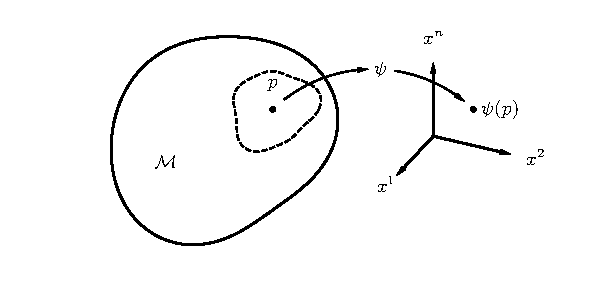
\includegraphics[width=4in, height=2in]{images/psimapping.pdf}
			\caption{Mapping of $p$ from a manifold $\mcal M$ to $\R^n$ via $\psi$}
			\label{fig:psimapping}
		\end{figure}

		This we often just write as $\{x^\alpha\}$, instead of saying $\psi$, which is fairly
		abstract; we just say $\qty{x^\alpha}$ and express it in terms of the coordinate functions.
		$\qty{x^\alpha}$ are the coordinate functions associated with $\psi$.
		\[
			\psi \iff \qty{x^\alpha}
		\]

		and once we have that we have our basis, which is expressed as a directional derivative
		in terms of the coordinate functions.
		\[
			\qty{\pdv{}{x^\alpha}}
		\]

		Often times, we will write this simply as
		\[
			\qty{\p_\alpha}
		\]

		When it's confusing, for example, when you have two different bases, we will write this differently.
		For example, if you have a different basis from a different chart $\qty{y^\alpha}$, we instead
		explicitly define each basis vector
		\[
			\psi_x \implies\qty{\pdv{}{x^\alpha}},\qquad \psi_y \implies \qty{\pdv{}{y^\alpha}}
		\]

		An example would be different representations of a vector in Cartesian coordinates in $\R^3$
		or spherical coordinates in $\R^3$. As a shorthand, we can also write
		\[
			\qty{\pdv{}{x^\alpha}}=\qty{\partial_\alpha},\qquad \qty{\pdv{}{y^\alpha}}=\qty{\partial'_\alpha}
		\]

		If there is confusion, like when there is a possibility that we're working on different charts, with
		two different sets of coordinate vectors, we can use this convention of having a primed operator.

		We also discussed last time that since it's a basis, I can now express any vector $\vb{v}_p$ in terms
		of any coordinate basis, so we can write, in terms of the $x$ chart,
		\[
			\vb{v}_p = 
			v_p^\alpha \partial_\alpha = 
			v_p^\alpha \pdv{}{x^\alpha}  
		\]

		Here, we said that $v_p^\alpha$ is really nothing but the action of $\vb{v}_p$ on the
		coordinate basis function $x^\alpha$. This is what we established last time.
		\[
			v_p^\alpha = \vb{v}_p(x^\alpha)  
		\]

		\begin{question}{So is $\partial_\alpha$ equivalent to the elementary basis vectors $\vb{e}_i$?}
			No, not all the time. They are kind of similar, but they are not quite the same. The elementary basis vectors
			in traditional physics are equivalent to them in Cartesian $\R^3$, simply
			a different way of writing
			\[
				\ihat, \jhat, \khat \equiv \pdv{}{x},\pdv{}{y},\pdv{}{z} 
			\]

			However, in other coordinate systems, this is not necessarily the case, because when we say
			something like $\vb{e}_\alpha$, then we are already saying something about the magnitude
			of these vectors, since these are unit and orthogonal vectors, whereas $\partial_\alpha$
			are not necessarily unit nor orthogonal because we do not have a notion of length here yet,
			and we do not have a notion of orthogonality as well. Those statements precede those notions.
			We can have coordinate basis vectors even without the notion of lengths, orthogonalities, or
			inner products. In Cartesian coordinates, these will turn out indeed to be equivalent once we introduce
			the so-called Euclidean metric. The Euclidean metric is what's going to provide us a sense of
			length and orthogonality, which is an inner product. Prior to that, without the metric, we already
			have coordinate basis vectors, but not the usual sense of lengths or orthogonality, which $\ihat$, $\jhat$, and $\khat$
			already contain.

			\hspace{1em}For example, the spherical basis vectors point in the same direction as $\partial_\alpha$, but they
			are not equivalent to the coordinate basis vectors you get from the manifold.
			\[
				\vu*{r}, \vu*{\theta}, \vu*{\phi}\not\equiv \pdv{}{r},\pdv{}{\theta},\pdv{}{\phi}  
			\]
			These are still coordinate basis vectors; it's very easy—you just take the coordinate and put it in the denominator,
			but they have (you will see this when we introduce the meaning of length) different
			magnitudes. Later on, when we introduce the notion of normalization and define a unit vector, then we recover the same vectors.
		\end{question}

	\subsubsection{Change of Coordinates}

		Now we proceed to the question that we left hanging in the last lecture.

		Suppose $p\in\mcal M$ belongs to two different charts, $\psi_1$ and $\psi_2$, and as such
		we have two different sets of coordinate functions that apply to and describe $p$.

		If that is the case, then we also have different sets of coordinate basis vectors on $\TpM$. It's
		the same $\TpM$, but for each chart, it can be described by two different sets of basis vectors, $\qty{x^\alpha}$ and $\qty{y^\alpha}$.
		So the question becomes: how do the different sets of components of $\vb{v}_p$ relate from one chart to another? Note that
		the components $v^\alpha$ are not the same as the vector $\vb{v}$. The components can change,
		but the vector remains the same.

\newpage
		\begin{figure}[h]
			\centering
			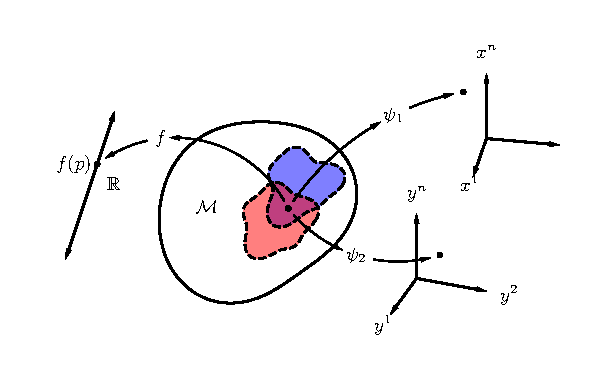
\includegraphics[width=4in,height=2.5in]{images/twocharts.pdf}
			\caption{Representation of a point $p\in\mcal M$ in coordinate basis charts $\qty{x^\alpha}$, $\qty{y^\alpha}$, and a scalar function $f$}
			\label{fig:}
		\end{figure}

		Notice that $x^\alpha$ is the $\alpha$th coordinate function on the chart $\psi_1$, since $\psi_1:p\mapsto x^\alpha$
		\[
			x^\alpha = \psi_1^\alpha(p)
		\]
		Similarly for $\psi_2$, we have
		\[
			y^\alpha = \psi_2^\alpha(p)
		\]

		We asked last lecture: how do we express a coordinate transformation from $y$ to $x$ in terms of $\psi_1$ and $\psi_2$? We find that
		\[
			y^\alpha (x^\beta) = (\psi_2 \circ \psi_1\inv)^\alpha(x^\beta)
		\]

		Now we want to understand how we define a vector present in both charts, and how its components relate to each other.

		To specify a vector, as we defined it in the last lecture, is to specify a map from functions to real numbers. We first need to define the map.
		Every vector is a derivative operator. If you tell me how it operates on a function, then you will have specified the vector.

		Suppose a vector on the $y$ basis at point $p$ is acting on a function. Recall how we defined this in the last lecture:
		\begin{equation}
			\qty( \pdv{}{y^\alpha})_p f = \eval{\pdv{f\circ\psi_2\inv}{y^\alpha}}_{\vb{y}_p}
			\label{eq:y-vector}
		\end{equation}
		Similarly, the $x$ coordinate vectors have exactly the same form.
		\begin{equation}
			\label{eq:x-vector}
			\qty( \pdv{}{x^\alpha})_p f = \eval{\pdv{f\circ\psi_1\inv}{x^\alpha}}_{\vb{x}_p}
		\end{equation}

		Notice that the definitions are exactly the same; the only difference is that we use the corresponding chart for each coordinate system.
		So, how do these things relate to each other? That's what we're trying to address.

		We can insert, in essence, an identity map $\psi\inv\circ\psi$
		\[
			\qty( \pdv{}{x^\alpha})_p f 
			= \eval{\pdv{f\circ\psi_2\inv \circ \psi_2 \circ\psi_1\inv}{x^\alpha}}_{\vb{x}_p}
		\]
		Then, we can just expand this out with standard multivariable calculus techniques, in particular
		we use the chain rule.

		\begin{question}{Is $\psi\circ\psi\inv$ also an identity?}
			Yes, it is also an identity map. However, we had to do it in this particular order for this derivation
			because we will not get the result we desire due to the non-commutative nature of
			these operators.
		\end{question}

		Proceeding with the operation, we find that
		\begin{equation}
			\pqty{ \pdv{}{x^\alpha}}_p f 
			=
			\eval{\pdv{(f\circ\psi_2\inv)}{y^\beta}}_{\vb{y}_p} \eval{\pdv{(\psi_2\circ\psi_1\inv)^\beta}{x^\alpha}}_{\vb{x}_p} 
			\label{eq:id-operator}
		\end{equation}

		Notice the change to $\vb{y}_p$. Since $f\circ \psi_2\inv$, as defined, is simply $f(\vb{y}_p)$, we evaluate from there.
		Now, what is $\psi_2\circ\psi_1\inv$? From the last lecture, as you can verify, this is just $\vb{y}(\vb{x})$, i.e., it
		can be represented as $y^\beta$.

		Also notice that we used another dummy index $\beta$. Since we used the chain rule, which sums over intermediate coordinates,
		we need to represent the intermediate coordinate index separately from the fixed
		$\alpha$, which labels the $x$-coordinate we are differentiating with respect to.

		Now we can represent (\ref{eq:id-operator}) as
		\[
			\qty( \pdv{}{x^\alpha})_p f 
			=
			\eval{\pdv{(f\circ\psi_2\inv)}{y^\beta}}_{\vb{y}_p} 
			\eval{\pdv{y^\beta}{x^\alpha}}_{\vb{x}_p} 
		\]

		But now, looking at this, we see that the first term is just (\ref{eq:y-vector}). This is nothing but
		\[
			\pqty{ \pdv{}{x^\alpha}}_p f 
			=
			\pqty{\pdv{}{y^\beta}}f \cdot 
			\eval{\pdv{y^\beta}{x^\alpha}}_{\vb{x}_p} 
		\]

		We can rearrange this because this is just multiplication, and $\displaystyle\eval{\pdv{y^\beta}{x^\alpha}}_{\vb{x}_p}$ are just numbers. Then
		\[
			\pqty{ \pdv{}{x^\alpha}}_p f 
			=
			\eval{\pdv{y^\beta}{x^\alpha}}_{\vb{x}_p} 
			\pqty{\pdv{}{y^\beta}}f  
		\]

		Notice that this is for an arbitrary function $f$, and as such, in an operational sense, we can write
		\begin{equation}
			\pqty{ \pdv{}{x^\alpha}}_p 
			=
			\eval{\pdv{y^\beta}{x^\alpha}}_{\vb{x}_p} 
			\pqty{{\pdv{}{y^\beta}}}_p
			\label{eq:chain-rule-result}
		\end{equation}

		One of the things that you will obviously see here is that this is nothing but the expression
		of the chain rule in multivariable calculus. It is as if we just wrote down the chain rule. It's very
		easy to remember. However, note that this has a different interpretation: we are giving a new interpretation
		to the chain rule. Because what is this statement actually telling you?
		What we're doing here is expressing the left-hand side, which is a vector, as a superposition, or a sum, over other
		basis vectors. So we are expressing a vector on the left-hand side as a linear combination of vectors on the right-hand side.

		So something like the chain rule, which is taken for granted in multivariable calculus because it is used so
		often, now gets a different interpretation in terms of vectors. The values on (\ref{eq:chain-rule-result}) are
		just numbers, so it's as if we are doing
		\[
			\ket{\psi} = \psi^i \ket{e_i}
		\]
		or a matrix multiplication
		\[
			\vb{x} = \vb{M}\vb{y}
		\]

		We interpret (\ref{eq:chain-rule-result}) as the following: The $\alpha$th basis vector in the $x$-coordinate system
		is a linear combination of the basis vectors in the $y$-coordinate system. Similarly, you can express
		\[
			\eval{\pdv{}{y^\alpha}}_p =  
			\eval{\pqty{
				\pdv{x^\beta}{y^\alpha} 
			}}_{\vb{y}_p} 
			\pqty{{\pdv{}{x^\beta}}}_p
		\]

		So it means that we can represent one basis in terms of the other. So how then do
		we relate the different components coming from these basis vectors?

		What we did earlier was that, given two sets of basis vectors, we asked how to relate one in terms
		of the other.

		By the way, the expressions $\displaystyle\pdv{y^\beta}{x^\alpha}$ are Jacobians; this is often called the tangent map,
		which we will explain later on. This is actually the partial derivatives of the transition functions, which are defined
		to be smooth in smooth manifolds.

	\subsubsection{Vector Transformation Laws}

		If I have a vector $\vb{v}_p \in \TpM$, and I have two different charts, then I get
		to represent this vector using two different sets of basis vectors. I can say that
		\begin{equation}
			\vb{v}_p = v_p^\mu \pdv{}{x^\mu}
			\label{eq:vpx}
		\end{equation}

		or we can write the same vector as
		\begin{equation}
			\vb{v}_p = {v'_p}^\nu \pdv{}{y^\nu}
			\label{eq:vpy}
		\end{equation}

		The important thing here is that we are talking about the same vector. Just like we can represent the vectors
		in different ways in different coordinate systems
		\begin{align*}
			\vb{v} &= v_x \ihat + v_y \jhat + v_z \khat\\
			\vb{v} &= v_r \vu*{r} + v_\theta \vu*{\theta} + v_\phi \vu*{\phi}
		\end{align*}

		Since they are the same vector, then we can equate (\ref{eq:vpx}) and (\ref{eq:vpy})
		\[
			{v'_p}^\nu \pdv{}{y^\nu}
			=	
			{v_p}^\mu \pdv{}{x^\mu}
		\]

		But we can express $\displaystyle\pdv{}{y^\nu}$ in terms of the coordinate basis vectors in $x$, as we have shown
		\[
			{v'_p}^\nu
			\pqty{
				\pdv{x^\mu}{y^\nu}
				\pdv{}{x^\mu} 
			}
			=	
			{v_p}^\mu \pdv{}{x^\mu}
		\]

		Though remember, the mnemonic is that of the chain rule. Functionally, this is different: it is a linear combination of the basis vectors.
		Proceeding, we can move the LHS to the RHS, and we find
		\[
			\pqty{
				v'_p \pdv{x^\mu}{y^\nu} - v_p^\mu
			}
			\pdv{}{x^\mu}
			=
			\vb{0}
		\]

		Now we invoke the fact that we proved last lecture: that $\displaystyle\pdv{}{x^\mu}$ is
		a basis, so the vectors are linearly independent. If the sum of the
		coefficients and the vectors is the zero vector, then the components inside the
		parentheses are equal to zero. Hence
		\[
			{v'}_p^\nu \pdv{x^\mu}{y^\nu} - v_p^\mu
			=
			0
		\]

		As such we can write
		\begin{equation}
			{v_p}^\mu = 
			{v'}_p^\nu \pdv{x^\mu}{y^\nu}  
			= 
			{\pdv{x^\mu}{y^\nu}} {v'_p}^\nu
			\label{eq:vpp-to-vp} 
		\end{equation}

		Similarly, we can express (\ref{eq:vpp-to-vp}), by inverting the
		argument and taking the reciprocal of the derivative as
		\begin{equation}
			{v'_p}^\nu = 
			\pdv{y^\nu}{x^\mu} v_p^\mu 
			\label{eq:vp-to-vpp}
		\end{equation}

		So this is how the components of the vector $\vb{v}_p$ relate to one another under
		a change of basis; this is a component transformation.

		Some of you will recognize this as the Arfken\cite{Arfken1985} standard definition of a vector. In fact, it is a contravariant vector.
		This is the old-fashioned definition of a contravariant vector. This is what's being taught by Arfken and a lot
		of other elementary or introductory physics books. We say old-fashioned because this is how it has traditionally been done
		before, but for us it is insufficient. For most physicists and most physics work, it is probably sufficient, but it doesn't
		really answer what a vector is, in a rigorous sense.

		If you ask ``What is a vector?'', a physicist would say, ``Well, if its components transform this way, it's a vector'' or ``It's an element of a vector space'', without
		really saying or answering what a vector is. So now, we know what a vector is: it's a derivative
		operator, and as a consequence of that, its components transform in a manner described by (\ref{eq:vp-to-vpp}).

		So this is no longer the definition of a contravariant vector; it is the transformation rule arising from the fact that
		vectors are derivative operators. For classical physics, it is generally sufficient to say how it transforms, but the problem is
		in GR and, in fact, for most of physics, we are emphasizing the geometric object itself, defining
		what the object is rather than how its components transform under different coordinate systems.

		We are trying to divorce ourselves from coordinates as much as possible. We are trying to work with the geometric objects themselves.
		Now we say it is a contravariant vector because there is a different kind of vector which is a covariant vector.

	\subsubsection{Contravariant and Covariant Vectors}

		A contravariant vector is as defined earlier. The appropriate transformation for such a vector is
		\[
			{v'_p}^\nu = \pdv{y^\nu}{x^\mu} v_p^\mu.
		\]

		It is called a contravariant vector because its components transform inversely (or ``contra") to the basis
		vectors. Recall that the basis vectors themselves transform as
		\[
		\pdv{}{x^\alpha} = \pdv{y^\beta}{x^\alpha} \pdv{}{y^\beta},
		\]
		so the basis vectors in the new coordinate system are related to the old ones by the same Jacobian matrix.
		The components, however, use the inverse Jacobian:
		\[
			v^\mu = \pdv{x^\mu}{y^\nu} v'^\nu.
		\]

		This ``opposite" transformation behavior—basis vectors transforming one way and components transforming the
		inverse way—is the origin of the term ``contravariant." The components are said to transform contravariantly.

		In contrast, a covariant vector (or one-form) has components that transform in the same way as the basis vectors.
		If you have a covariant vector $\omega_p$, the transformation rules are expressed as
		\begin{equation}
			\label{eq:covariantvectordef}
			(\omega_p)'_\nu = 
			\pdv{x^\mu}{y^\nu} \pqty{\omega_p}_\mu 
		\end{equation}

		This is the definition of a covariant vector. But later on, in a couple of lectures from now,
		we will see that we will no longer call these vectors. These are actually going to be one-forms.
		Something which transforms like (\ref{eq:covariantvectordef}) is called a one-form, or alternatively, a
		dual vector.
		We will explore these in much greater detail in the next meeting. For now, it suffices to recognize that contravariant 
		vectors are what we traditionally think of as "arrows" or tangent vectors, while covariant vectors are linear functionals 
		that act on them to produce real numbers—the natural generalization of the dot product or inner product in a coordinate-free setting.

		This distinction will become crucial when we introduce metrics and begin to discuss how to raise and lower indices,
		compute lengths, and define angles in curved spacetime. But those are topics for future lectures

		So that we aren't so confused, we have encountered these in physics before, a contravariant vector is equivalent to a \textit{ket},
		\[
			\ket{\psi}
		\]
		and a covariant vector is equivalent to a \textit{bra}
		\[
			\bra{\phi}
		\]

		We do not say that bras and kets are the same. Of course, they are isomorphic, but they
		are quite different. They serve different purposes.
		Covariant and contravariant vectors are usually defined in terms of how they
		transform in physics, but we will define these other vectors later on, when we discuss one-forms.
\newpage
	\subsubsection{Non-Coordinate Bases}

		Now it's important to emphasize that $\TpM$ is a vector space. You don't always need coordinate basis vectors for vector spaces.
		In fact, later on we will find that it is quite practical and useful to adopt non-coordinate basis vectors.

		So the vector basis need not be coordinate basis vectors; in other words, they don't need to come from a coordinate system or a chart
		because it's a space, you can put in a plethora, an infinite number of basis vectors on it.

		For example, you have a set of basis vectors; you will need $n$ of them if you have an $n$-dimensional manifold, and
		they will have some components with respect to some basis, and these bases need not come from
		a coordinate system; they can be linear combinations of coordinate basis vectors.
		\[
			e_{(\beta)} = e_{(\beta)}^\alpha \pdv{}{x^\alpha} 
		\]

		The only constraint is
		that it must have a nonzero determinant. You don't get a basis unless the matrix formed by the basis vectors
		has a nonzero determinant. It must be nonsingular; otherwise, you do not have a basis.

		Later on, when we go to Lie derivatives, we will investigate under what conditions $e_{(\beta)}$ will actually have a coordinate representation.
		The short answer is that the Lie derivative should be zero.
		\[
			\mathscr{L}_{(\beta)} e_{(\alpha)} = 0
		\]

		If this is true for any $\alpha$ and $\beta$ for this new set of basis vectors that we've introduced, then
		there is a set of coordinates for which these are coordinate basis vectors. I can find a coordinate system to write,
		for example:
		\[
			e_{\beta} = \pdv{}{z^\beta} 
		\]

		If the Lie derivative condition is satisfied, but we'll get to that much later on.
\newpage
	\paragraph{Recovering the Geometric Arrow}

		So now, we want to be able to recover the notion of an arrow in $\R^n$. So far, we've had a lot of properties
		that we have sort of found and recovered in what we understand to be traditional vectors in physics. But to really get
		a sense of an arrow, we need to talk about curves and tangent vectors.

\subsection{Curves and Tangent Vectors}
	\subsubsection{Curves}

		We feel like we have a notion or sense of what a curve is, since we encounter it in physics
		a lot. However, for our purposes, we need to precisely define what a curve is.
		\begin{definition}{Curves}
			A curve $C$ in a manifold $\mcal M$ is a map from an open interval $I\subset\R$
			onto $\mcal M$
			\begin{equation}
				\label{eq:curvedef}
				C:I \to \mcal{M}
			\end{equation}
		\end{definition}
		\begin{figure}[h]
			\centering
			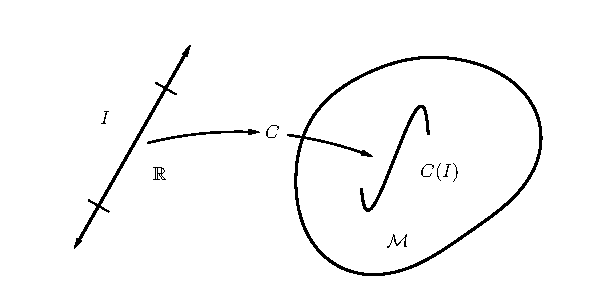
\includegraphics[width=4in,height=2in]{images/curve_in_a_manifold.pdf}
			\caption{A curve mapping a real line interval to a manifold}
			\label{fig:curve-in-a-manifold}
		\end{figure}

		$C(I)$ is a function, which is different from how we usually imagine a curve, which is
		some line with a curvature on $R^n$. $C(I)$ is not actually the curve itself, but
		the image of the curve. So what we tend to think of as the curve is really the image
		of the curve $C$, because $C$ itself is the map; $C$ is the function. It's the instruction manual that tells
		us how to relate a real number to a point in $\mcal M$, i.e., $C:\R\mapsto p$. $C(I)$ is a set of points in $\mcal M$.
		And $I\subset \R$ is called a parameterization. $I$ need not be a proper subset; it can be the entire real line. It is how we parameterize a curve. Say, for example, you want to think of the parameter
		$I$ as time, $t$, which is a very typical parameter in physics; the parameter need not be uniform. People can have different parameterizations,
		different clocks running at different rates, for instance.

		Imagine a different curve, say $C':I'\to \mcal{M}$, with different parameters $I'$, such that
		\[
			C(I)= C'(I')
		\]
		then we call these curves to have the same image, but different parameterizations. So we often say
		that $C$ and $C'$ are reparameterizations of each other. They have the same image, the same set of points,
		but the parameter $I$ that maps it is different, i.e., $C'(t')\neq C(t)$.

		If they are reparameterizations of each other, then it is not so strange that there will exist an onto map,
		a surjective map $\alpha: I \to I'$, such that
		\[
			\alpha(t)=t'
		\]
		and
		\[
			C = C'\circ \alpha
		\]

		An important thing to emphasize here is that a curve on its own does not need coordinates.
		It's a map from the subset of the real line to the manifold. However, in physics, it's very common
		to express curves in terms of coordinates, which we can do on manifolds by mapping the points
		$C(I)$ to $\R^n$. Pictorially, we
		can represent this as
		\begin{figure}[h]
			\centering
			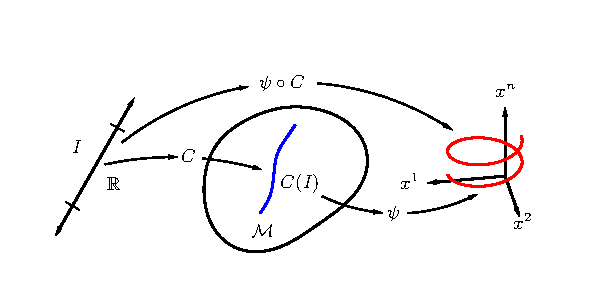
\includegraphics[width=4in,height=2in]{images/curves-chart.pdf}
			\caption{$\psi:C(I)\to \R^3$}
			\label{fig:cuves=chart}
		\end{figure}

		As such, we can recover the normal parameterization of a real number as a coordinate in $\R^n$.
		\[
			\psi\circ C: I \to \R^n
		\]
		Recall that $I\subset\R$, therefore $\psi\circ C:\R\to\R^n$. In other words
		\[
			\psi\circ C: t \mapsto x^\alpha(t)
		\]

		This is simply the usual sense of parameterization of a curve. For example, $[x(t),y(t),z(t)]$, which is how we normally describe curves in physics.
		You can provide a coordinate representation of curves, but the curve itself actually did not require
		the coordinates. So what we do is coordinatize a curve.

	\subsubsection{Coordinate Curves}

		There are going to be these special curves which we need to define. Given some chart, which we represent with $\qty{x^\alpha}$,
		consider the following subsets of open sets in $\mcal M$ for which the coordinates are valid, with chart $\psi$, and atlas $\qty{\mcal{O},\psi}$. Consider the following
		subset of all points in $\mcal{O}$ such that
		\[
			\qty{
				p\in\mcal{O} : 
				x^2(p) = \text{constant, }
				x^3(p) = \text{constant, }
				\ldots
				x^n(p) = \text{constant }
			}
		\]

		What do you imagine these sets of points to be? The image of this map is a straight line at $x^1(p)$, because we are keeping all the $x^\alpha$'s constant, except
		for $x^1$. However, the set that we're looking at, since it's a set of all $p$'s in $\mcal O$, is the pre-image of the
		points that will get mapped into a line. So this set is asking you to imagine what points in $\mcal O$ will get mapped into a
		straight line by $\psi$.

		\begin{figure}[h]
			\centering
			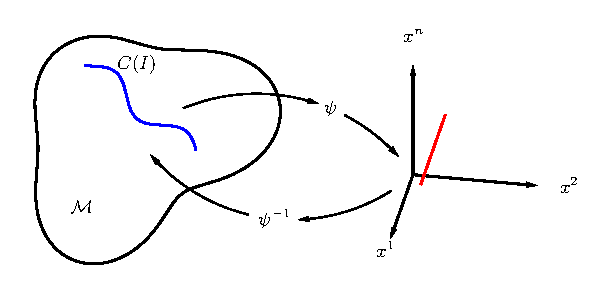
\includegraphics[width=4in,height=2in]{images/specialcurves.pdf}
			\caption{Curve on $\mcal M$ mapped to $\R^n$, resulting on a curve with only $x^1$ varied, and the rest of $x^\alpha$ constant}
			\label{fig:specialcurve}
		\end{figure}

		So with this set, consider the inverse map $\psi\inv$; it defines a set of points that will get mapped to a straight line. Since we know it is continuous,
		then that necessarily means that the pre-image is a continuum of arbitrary points, i.e., the preimage is a curve on the manifold, because it's mapping an
		open interval of $\R$ onto a set of points in $\mcal M$. This is a special type of curve; it's called the $x^1$ coordinate line or $x^1$ coordinate curve.
		Notice here that the parameter is $x^1$. This is an important notion.

		The $x^1$ coordinate curve is the image of a curve on the manifold whose parameter is the $x^1$ coordinate.

		We can then imagine, instead, doing the same for a line where $x^2$ is a parameter, then $x^3$, and so on, until $x^n$. What you then form then
		is a map of the correspondences of each axes or coordinate basis in the chart to a curve on the manifold itself, a set of curves on the manifold
		that correspond to each coordinate axes of the chart. You are therefore,
		placing a reference grid on how points on the manifold will map to $\R^n$ when $\psi$ is applied.
		Each point $p$ on the chart lies at the intersection of exactly $n$ coordinate curves, one for each coordinate direction.
		The coordinate curves depend entirely on the choice of chart. A different chart will generally produce a different set of curves on the manifold

		A second property is that the tangent vector, which is a vector that we will define later for curves, of the coordinate curves
		form a coordinate basis. The tangent vector to the $x^\alpha$ coordinate curve at $p$ is precisely the coordinate
		basis vector $\p_\alpha$. 

		If you imagine a manifold as a curved surface embedded in higher-dimensional space, then coordinate curves are
		the grid lines drawn on the surface. The tangent vectors to these curves are the arrows that point along the grid lines. 
		Any tangent vector can then be thought of as a linear combination of these grid-line arrows.

	\subsubsection{Tangent Vectors at Curves}

		You have an intuitive sense of what a tangent vector is: it's the arrow that points in the direction
		instantaneously of the curve. In a sense, a tangent vector is our traditional notion of what a tangent vector is.
		But because it's a vector, we now know that it's supposed to be a directional derivative.
		We have to appropriately define, then, a tangent vector as a derivative operator.

		\begin{figure}[h]
			\centering
			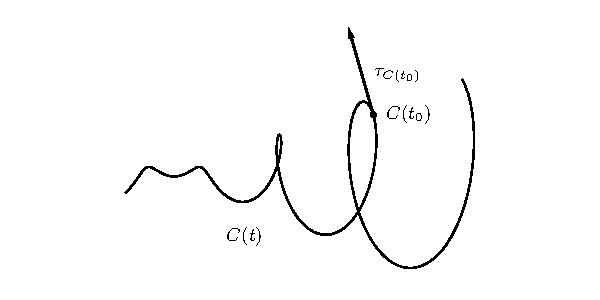
\includegraphics[width=4in,height=2in]{images/tangentvectors.pdf}
			\caption{Tangent vector $\tau$ on a curve $C(t)$}
			\label{fig:tangentvectors}
		\end{figure}

		It's always associated with a curve; i.e., if there's a curve, there must be a tangent vector. We define it then as such.

		\begin{definition}{Tangent Vector at Curves}
			If $C(t)$ is a curve, then the tangent vector $\tau$ at $C(t_0)$ is the derivative operator
			such that $\tau_{C(t)}$ acting on an arbitrary function $f$, is defined to be
			\begin{equation}
				\label{eq:tangent_vector}
				\tau_{C(t_0)} (f) = 
				\eval{\dv{(f\circ C)}{t}}_{t_0}
			\end{equation}
		\end{definition}
	
		Now we ask, what is the nature of the object that results from this definition? What are its properties?
		What is the map $f\circ C$? Remember that $f$ is a map from the manifold to real numbers, and $C$ is a map
		from real numbers to the manifold. So $f\circ C$ is a map from real numbers to real numbers.
		\[
			f\circ C : \R \to \R
		\]

		So it's
		simply a normal function, a perfectly sensible real function, which hass a derivative
		with respect to a parameter.

		Notice that the definition of a tangent vector requires a curve. If you have the same curve $C$,
		but evaluate it at another parameter $t_1$, then it makes a different tangent vector acting on
		the same function, but evaluated at a different point.
		\[
			\tau_{C(t_1)} (f) = 
			\eval{\dv{(f\circ C)}{t}}_{t_1}
		\]

		This is a different tangent vector. We can show that this is in fact a vector as we previously defined it, i.e.,
		it must satisfy linearity and the Leibniz property, but by the nature of the function, since it's a derivative operator, it obviously
		satisfies both. This definition satisfies the properties of being a vector, or being a derivation. We will recover the notion
		of an arrow from this; this is where the traditional arrow definition of a vector comes from.
		Here, we only define it. We shall discuss it in detail in the next meetings.
		\begin{proof}
			For $a,b\in\mathbb{R}$ and $f,g\in C^\infty(M)$,
			\begin{align}
				\tau_{C(t_0)}(af+bg)
				&=
				\eval{\dv{}{t}\bigl((af+bg)\circ C\bigr)}_{t_0} \notag\\
				&=
				a\eval{\dv{(f\circ C)}{t}}_{t_0}
				+b\eval{\dv{(g\circ C)}{t}}_{t_0} \notag\\
				&=
				a\tau_{C(t_0)}(f)+b\tau_{C(t_0)}(g),
			\end{align}
			so it is linear.

			For $f,g\in C^\infty(M)$,
			\begin{align}
				\tau_{C(t_0)}(fg)
				&=
				\eval{\dv{((fg)\circ C)}{t}}_{t_0} \notag\\
				&=
				\eval{\dv{}{t}\bigl((f\circ C)(g\circ C)\bigr)}_{t_0} \notag\\
				&=
				\eval{\qty[
					(g\circ C)
					\dv{(f\circ C)}{t}
					+
					(f\circ C)\dv{(g\circ C)}{t}
				]}_{t_0} \notag\\
				&=
				\tau_{C(t_0)}(f)g(C(t_0))
				+
				f(C(t_0))\tau_{C(t_0)}(g).
			\end{align}
			Thus $\tau_{C(t_0)}$ is a derivation at $C(t_0)$, and hence, a vector.
		\end{proof}

		\newpage
		% =======================================
% MEETING 7
% ---------------------------------------
% DATE   - September 11, 2026
% FORMAT - Online
% =======================================
% TOPIC  - Tangent vectors
% =======================================

\subsection{Tangent Vectors}

	We begin with what we learned last time.
	We already defined the notion of a vector on a manifold.
	This entails the notion that if you have a map $V$ belonging
	to a so-called tangent space, $V\in\TpM$, then this is a map from
	smooth functions to real numbers:
	\[
		V: \mcal{F} \to \R
	\]
	We also learned that if you have a chart, represented by ${x^\mu}$,
	then you can always represent a vector as a linear combination of
	the so-called coordinate basis vectors, which we represent in the following way:
	\[
		v_p = v_p^\mu \eval{\pdv{}{x^\mu}}_p
	\]
	Here, $v^\mu$ are the components, and $\pdv{}{x^\mu}$ are the basis vectors
	at a point $p$ on the manifold. At each point $p$, there exists a tangent space.
	\begin{figure}[h]
		\centering
		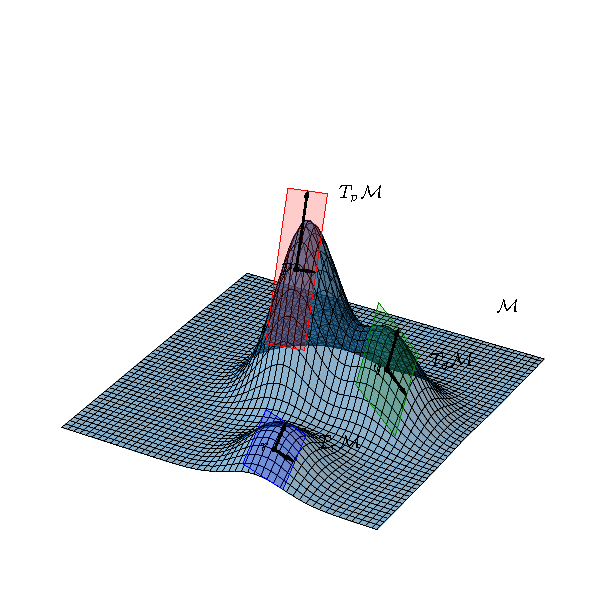
\includegraphics[
			width=4in,
			trim = {0cm 1cm 0cm 3cm},
			clip
			]{images/tangentspaces.pdf}
		\caption{Tangent spaces at points $p$, $q$, and $r$ in an arbitrary manifold $\mcal M$.
			The arrows are the respective basis vectors on the embedding axes.}
		\label{fig:tangentspacesonpoints}
	\end{figure}

	We also say that $\TpM$ is a vector space. The key point here
	is that we need to differentiate $\TpM$ from the manifold $M$ itself.
	$\TpM$ is the space of all vectors that live at $p$, which is not necessarily
	the same thing as $M$.

	This is what makes differential geometry confusing because when we learn
	elementary differential geometry, we often learn it in the context of
	$\R^2$ or $\R^3$. In $\R^2$, the manifold is $\R^2$ itself, so when you get
	a tangent space at a point $p$, call it $T_p\R^2$, which is the space of
	all derivative operators at $p$, then the tangent space is isomorphic to
	$\R^2$ itself. This is why we confuse positions in $\R^2$ with vectors.
	However, in general, that is not the case.

	In this lecture, we will be covering the notion of a tangent vector associated
	with curves on a manifold. Our usual notion of tangency, which is something
	like a tangent line or a tangent plane to curves or surfaces in $\R^2$ or $\R^3$,
	will be recovered as the same notion, but defined more precisely in terms
	of a tangent vector.

	We will draw out a very important distinction between the tangent space
	$\TpM$ and the manifold $\mcal{M}$ itself, which can very often be lumped
	together and confused because $T_p\R^n$ is isomorphic to $\R^n$, which
	is how it is introduced. That is, we have barely any distinction
	between a position vector and a position. For example, say we have a point
	$p$ defined by $(x,y)\in\R^2$. We can then think of a vector
	$(x,y)_p\in T_p\R^2$, and there is really no clear distinction between the two.
	It is important to understand that, in general, manifolds and tangent spaces
	are really different things.

	\subsubsection{Tangent Vector Components}

		We introduce a shorthand when writing down components. In general, a vector
		$v_p$ can always be written in terms of its components
		$v_p^\mu \pdv{}{x^\mu}$, given a chart and the coordinate basis vectors
		coming from that chart. However, these components are just numbers,
		plain real numbers:
		\[
			v_p^\mu\in\R
		\]
		We can compute them easily by having the vector itself $v_p$ act
		on the coordinate functions. That is,
		\begin{equation}
			\label{eq:vectoract}
			v_p^\mu = v_p[x^\mu]
		\end{equation}
		This is a perfectly well-defined operation, since $v_p$ can act on functions,
		and such an operation results in a real number. How can we see that this is true?
		\begin{proof}
			A vector $v_p$ can be written in general as
			\[
				v_p = v_p^\nu \pqty{\pdv{}{x^\nu}}_p
			\]

			We can make this vector act on a coordinate function $x^\mu$:
			\[
				v_p[x^\mu]
				= v_p^\nu \qty(\pdv{}{x^\nu})_p x^\mu
			\]

			Remember how the basis vector operates on functions. To this effect,
			we have
			\[
				v_p[x^\mu]
				= v_p^\nu \qty(\pdv{x^\mu}{x^\nu})_p
			\]

			However, by definition,
			\[
				\pdv{x^\mu}{x^\nu}
				= \tensor{\delta}{^\mu_\nu},
			\]
			therefore
			\[
				v_p[x^\mu]
				= v_p^\nu \tensor{\delta}{^\mu_\nu}
			\]
			Which is just
			\[
				v_p[x^\mu] = v_p^\mu
			\]

			So these components can be obtained by making the vector
			act on the coordinate function.
			\footnote{
				From here on, we use the following convention. For operators, brackets
				$[\cdot]$ indicate that the operator is acting on something, while
				parentheses $(\cdot)$ denote that they depend on something.
			}
		\end{proof}

		We are later going to use this shorthand in our calculations.

		Taking from where we left off in the previous lecture, we discussed
		curves, which are maps from an open interval $I\subseteq\R$ to the manifold,
		i.e.,
		\[
			C:I\to\mcal{M}
		\]

		So if we have a chart, ${x^\mu}$, then a curve is parameterized in $\R^n$ as
		\[
			\psi\circ C \iff x^\mu(t),
			\qquad t\in I\subseteq\R
		\]
		Recall, however, that this is a parameterization. The curve itself is independent
		of the parameterization. Given a curve, we can define a tangent vector.
		If $C(t)$ is a curve, then we define the tangent vector associated with this
		curve as
		\[
			\tau(f) = \eval{\dv{(f\circ C)}{t}}_{t_0}
		\]
		Sometimes, this tangent vector $\tau$ is denoted as
		\begin{equation}
			\label{eq:tauatc}
			\tau = \eval{\pdv{}{t}}_{C(t_0)}
		\end{equation}
		That is, it is a vector at the point $C(t_0)$ that is able to act on functions,
		and it does so precisely as we defined it.

		This is a familiar operation because these are just a set of numbers,
		and we take a derivative of them with respect to $t$. It is a normal derivative
		associated with the point $C(t_0)$.

		Recall that we also previously defined a set of special curves called the
		$x^\mu$ coordinate lines. These are curves which, when mapped by $\psi$
		to $\R^n$, only vary one component while allowing the rest to remain constant.
		It is the image of a curve with parameter $x^\mu$. In effect, since we have
		an association between these sets of points in the image of $C$, $x^\mu$
		becomes a parameter on this curve. It serves as the $t$, so to speak.
		As we vary $x^\mu$ in $\R^n$, the corresponding preimage on the manifold
		also varies. Therefore, we can effectively express this coordinate curve as
		\[
			C(x^\mu)
		\]
		Since $\psi$ is a one-to-one map, its inverse preserves the correspondence
		between curves in the coordinate domain and curves on the manifold. For example,
		if we have $C(x^1)$ and $C(x^2)$, those two curves should be independent
		and will not overlap in the coordinate domain. Each coordinate line in $\R^n$
		will correspond to a different coordinate curve on the manifold, and each
		coordinate serves as a parameter for its corresponding family of curves.
		If this correspondence were not one-to-one, $\psi$ would not be a valid chart.

		Note that we are not just choosing any arbitrary line in $\R^n$. We are choosing
		lines which preserve the other coordinates $x^\nu$, while only varying $x^\mu$.
		For example, consider the polar-coordinate pair $(r,\theta)$. The coordinate
		domain for polar coordinates is a subset of $\R^2$, with
		\[
			r\in[0,\infty),
			\qquad
			\theta\in[0,2\pi).
		\]

		When we map coordinate lines to a manifold, say a ball, we map these lines of
		constant values such that the other coordinates remain fixed while only one
		is allowed to vary. Say we want to map a coordinate line for $\theta$.
		We select a value of $r$, keep it constant, and allow $\theta$ to vary.
		This would be a $\theta$-coordinate line.

		It is not the only $\theta$-coordinate line; there are multiple coordinate
		lines for each coordinate, as long as the other coordinates are held fixed
		and the corresponding coordinate is varied. In this way, we are effectively
		putting a \textit{grid} on the manifold, which corresponds to lines of constant
		values in the coordinate domain.
		\begin{figure}[h]
			\centering
			\includegraphics[width=3in]{polarcoordline.pdf}
			\caption{Coordinate curves of the polar coordinate basis}
			\label{fig:polarcoordline}
		\end{figure}

		Each coordinate is therefore associated with a family of coordinate lines.
		Now that the notion of coordinate curves is understood, and tangent vectors
		are associated with curves, we can then assign tangent vectors to these
		coordinate curves.

		Given an $x^\mu$-coordinate line, with $x^\mu$ as the parameter, it is
		common to denote the tangent vector at a point $p$ as
		\begin{equation}
			\label{eq:tangentvector on a curve}
			\eval{\pdv{}{x^\mu}}_{p} [f]
			= \eval{\pdv{f(x^\mu)}{x^\mu}}_{x^\mu(p)}
		\end{equation}
		with $f$ being an arbitrary function evaluated on the curve.\footnote{
			Recall that when we say $f$, what we really mean is
			$f\circ\psi\inv$, i.e.,
			$f(x) \equiv (f\circ\psi\inv)[x]$.
		}
		We are taking a derivative with respect to the $x^\mu$ parameter.

		Notice that the tangent vector that we wrote in
		(\ref{eq:tangentvector on a curve}) is the same as the definition
		that we used for coordinate basis vectors. This particular definition
		of the tangent vector on a coordinate curve precisely coincides with the
		previous definition of coordinate basis vectors, which we denote in the same way.

		This then implies that coordinate basis vectors are tangent vectors.
		They are tangent vectors associated with the $x^\mu$ coordinate curve.
		They are one and the same.

		We defined vectors previously as simply an abstract notion, but here,
		we recover what we mean by a vector. A coordinate basis vector is simply
		the tangent vector to a coordinate curve, whose components describe the
		rate of change of the coordinates along that curve, and whose direction
		corresponds to increasing $x^\mu$.

		Let's bring this definition a little bit more down to earth. Consider
		$x^\mu(t)$ to be the parametric equations for a curve, i.e., we now use
		coordinates to represent the abstract curve. Let's then consider the action
		of a tangent vector $\tau$ associated with $C(t_0)$ on an arbitrary function $f$:
		\[
			\eval{\pdv{}{t}}_{C(t_0)}f
			= \eval{\dv{f(C(t))}{t}}_{t_0}
		\]

		What we will do is find an expression for this tangent vector that uses the chart.
		We can rewrite this as
		\[
			\eval{\pdv{}{t}}_{C(t_0)}f
			= \eval{\dv{(f\circ\psi\inv\circ\psi\circ C)}{t}}_{t_0}
		\]
		We recall that
		$f\circ\psi\inv:x^\mu\mapsto f\circ\psi\inv(x^\mu)=f(x^\mu)$,
		which is how we represent the function $f$ in coordinates, and
		$\psi\circ C:t\mapsto x^\mu(t)$, which is the parametric form for the curve.
		It looks complicated, but this entire expression is nothing but the following:
		\[
			\eval{\pdv{}{t}}_{C(t_0)}f
			= \eval{\dv{f(x^\mu(t))}{t}}_{t_0}
		\]
		This is just normal calculus. We just use the chain rule:
		\[
			\eval{\pdv{}{t}}_{C(t)} f
			= \eval{\dv{x^\mu}{t}}_{t_0}
				\eval{\pdv{f}{x^\mu}}_{x^\mu(C(t_0))}
		\]
		We rearrange things a bit. Notice that the second term on the right-hand side
		is nothing but (\ref{eq:tangentvector on a curve}). Recall here that
		$p=C(t_0)$. As such, we can write it as the coordinate basis vectors acting on $f$:
		\[
			\eval{\pdv{}{t}}_{C(t_0)} f
			= \eval{\dv{x^\mu}{t}}_{t_0}
				\eval{\pdv{}{x^\mu}}_{x^\mu(C(t_0))} f
		\]
		Since $f$ is arbitrary, we can remove it, and hence we find that
		\begin{equation}
			\label{eq:curve as basis}
			\eval{\pdv{}{t}}_{C(t_0)}
			=
			\eval{\dv{x^\mu}{t}}_{t_0}
			\eval{\pdv{}{x^\mu}}_{x^\mu(C(t_0))}
		\end{equation}

		Recall that this is a tangent vector associated with a curve $C$ at $t_0$,
		and we have now written it down as a linear combination of basis vectors.
		This shows that any tangent vector can be written as a linear combination
		of coordinate basis vectors. Therefore, a tangent vector is a vector in
		the tangent space, represented as a derivation acting on smooth functions.

		Not only that, but the components of the tangent vector are
		\[
			\dv{x^\mu}{t},
		\]
		which is exactly what we understand a tangent vector to be in the usual
		geometric parameterization sense: something analogous to a \textit{velocity},
		the rate of change of the coordinates $x^\mu$ with respect to $t$.

		The distinction here is that what we used to call a tangent vector in a
		mechanical sense is not actually the tangent vector itself; rather,
		$\dot{x}^\mu$ are the components of the tangent vector:
		\[
			\underbrace{\eval{\pdv{}{t}}_p}_{\text{tangent vector}}
			=
			\underbrace{\dv{x^\mu}{t}}_{\text{components}}
			\underbrace{
				\eval{
					\pdv{}{x^\mu}
				}_p
			}_{\text{basis vectors}}.
		\]
		The components require a coordinate system, or a chart. The tangent vector
		itself is independent of the choice of coordinates, but the values of its
		components will change depending on the chart you choose. The tangent vector
		itself does not change; it is a geometric object associated with the curve.
		We are drawing a distinction between coordinate expressions and the object itself.

		So a tangent vector is a vector, which may seem obvious. However, what is
		perhaps more surprising is that directional derivatives themselves are
		tangent vectors.

		\noindent\textit{Exercise: All directional derivatives are tangent vectors.}

		It suffices to show that if you have a derivative operator $v$ acting on
		$f$ at a point $p$, $v[f]$, I can always associate a curve on the manifold
		which passes through $p$, such that we can use that curve to define the same
		tangent vector. Thus, we can always associate a curve with a tangent vector
		at point $p$.
		You should be able to find a curve such that
		\[
			v[f] = \dv{[f(C(t))]}{t},
		\]
		where $v$ is an arbitrary vector acting on an arbitrary $f$. When you have
		shown that, then you have shown that any vector can be associated with some
		curve, and we can do this by invoking the uniqueness of solutions to
		differential equations.

		\begin{question}{Are tangent vectors similar to velocities since it's represented as $\dot{x}^\mu$?}
			The velocity itself, physical velocity, is a tangent vector.

			\hspace{1em}
			In usual physics, we usually refer to
			\[
				\dv{x^\mu}{t}
			\]
			as the velocity. However, the velocity \textit{components} can change
			with a change of chart and coordinates. But the velocity vector itself does not.

			\hspace{1em}
			The tangent vector is not something that depends on $x^\mu$; it is an
			abstract geometric object. $\dot{x}^\mu$ is not the tangent vector;
			it is just the components of the tangent vector. The vector itself is
			a geometric object that precedes the introduction of a chart.

			\hspace{1em}
			Prior to our discussions in this class, the usual way of thinking
			about tangent vectors was through coordinates. But how do we define
			things without coordinates?
			These definitions are precisely what we laid out: vectors are operators
			on functions. If you give a vector a chart, it will have components that
			are identical to how we used to think about tangent vectors.
		\end{question}

		When we do geometry, we are so used to using coordinates, and in this
		form of thinking, we are trying to define objects and geometry that are
		independent of our way of describing them. Geometry is not something
		which depends on how we choose to represent what axes we choose.
		Geometry has to be defined without recourse to coordinates.

		However, as physicists, we always calculate in coordinates for anything practical.
		I am not saying that we are completely going to devalue coordinates;
		we just need to be more careful with them and remember that there is an object
		that precedes the coordinate representation.

		GR is mostly about mindsets, and in this, we take the hierarchy of:
		geometrical objects, basis, components. It's not going to be that hard,
		but it does require a certain frame of mind, because how we define and
		manipulate things in physics is highly dependent on how we interpret and
		think about things.

		If we start with components, GR actually becomes harder. I could have taught
		you GR directly without doing any differential geometry: we could just say
		``these are the equations, these are how they're manipulated,'' and then
		solve the PDEs involved. However, without the foundations given to us by
		differential geometry, it is going to be very difficult to interpret the
		results we obtain.
		You can just compute it, you can put it in \texttt{mathematica} and do the
		calculations, and usually, that's where the bulk of the work comes from.
		But then, once you have a result, how do you think about the result?
		You have to go back to what it means geometrically.

		We always ask that question: What does this mean, geometrically?

		Now, for the rest of the lecture series, and from the previous definitions,
		we denote that there is not going to be any difference between vectors,
		tangent vectors, and derivative operators or derivations. They are all
		one and the same. When you refer to the geometric object with one of those
		names, you refer to all of them.

		You think about the class of curves that is associated with the operator,
		and how a derivation acts on functions.

	\subsubsection{Vector Fields}

		So obviously, tangent vectors at a single point are of limited utility
		in physics. When we do physics, what we really deal with are vector fields.
		So what is a vector field?

		In $\R^n$, a vector field simply means that you define a vector at every point
		in $\R^n$; it is a specification of a vector $v$ for all points $p\in\R^n$.

		A vector field on a manifold works in precisely the same way. It is a
		selection of a vector at every tangent space of a manifold. So if we have
		a manifold $\mcal M$ and take a point $p$, it is associated with a tangent
		space $T_p\mcal M$, and if we take a point $q\in\mcal M$, it is associated
		with a tangent space $T_q\mcal M$.

		At every point, there is going to be a tangent space that can be defined,
		which sort of \textit{sticks out} from the manifold.
		These tangent spaces are vector spaces; however, $\mcal M$ itself is not
		necessarily a vector space.

		Bear in mind that these tangent spaces do not intersect one another.
		We are used to thinking about vectors and planes being embedded in $\R^3$.
		However, in general, there is nothing that exists outside the manifold itself
		that we need to regard as an ambient space.

		Tangent spaces are abstract spaces. There is no ambient space around them
		that the tangent space is a subset of. The only geometric object we are
		assuming is the manifold. There is no intersection between tangent spaces
		at different points.

		We represent tangent spaces as planes because it is a convenient pictorial
		representation; it is easier to visualize. However, there is not really a
		plane in the usual sense. When we say a plane, we think of it as a subset
		of a bigger space. However, a tangent space is not a subset of a bigger
		space; it is simply an abstraction associated with each point on the manifold.
		That's a common misconception, and we wish to differentiate it.

		Moving on, the set of all tangent spaces constitutes the tangent bundle.
		More precisely, the tangent bundle is the disjoint union of all tangent spaces:
		\[
			T\mcal M = \bigcup_p T_p\mcal M.
		\]
		This is called the tangent bundle. A vector field is then a selection
		of a vector at each point, or equivalently, a section of the tangent bundle.

		\begin{definition}{Vector field}
			A vector field $v$ is a section of the tangent bundle $T\mcal M$, which assigns
			a vector $v_p$ for all $p$ in $\mcal{M}$.
		\end{definition}

		Let me explain why that's an appropriate terminology. Let's illustrate it
		with an easy example. Let's say $\mcal M$ is a one-dimensional manifold,
		$\R$. That means you can completely characterize it with one coordinate,
		a line, basically.

		So how would you represent a vector field on a line? How would one represent it?
		Say we have a variable $x$ representing points $p\in\R$. Let's say a vector
		field $v$ is a function of $x$:
		\[
			v(x).
		\]
		Recall that a vector is an operator. It acts on functions and returns
		a real number. A vector field, however, assigns a vector to each point.
		In a coordinate representation on $\R$, this can be described by a
		function of $x$.

		What we really think of then as a vector field is a collection of vectors
		associated with the points in $\R$. The corresponding functions are smooth,
		so the vector field varies smoothly from point to point; this is the usual
		setting of real analysis.
		\begin{figure}[h]
			\centering
			\includegraphics[width=4in, height=2in]{images/vectorfieldRtrad.pdf}
			\caption{A vector field on the $\R$ line}
			\label{fig:vectorfield}
		\end{figure}

		This vector field is just like a normal vector field: it is a bunch of arrows
		throughout. We make a mistake, though, because we think that vectors live
		on $\R$ as arrows. It is how we represent them.

		However, $v(x)$ really lives in a tangent space:
		\[
			v(x)\in T_x\R.
		\]

		However, $v$ does not live on $\R$; it just happens that $T_x\R$ is isomorphic
		to $\R$. What we usually do, then, is simply represent the vector itself
		as existing in $\R$.

		We would like to emphasize the fact that vectors live in tangent spaces,
		and so we represent them on another \textit{axis} instead, similar to how
		we treat complex numbers. We draw arrows like:
		\begin{figure}[h]
			\centering
			\includegraphics[width=4in, height=2in]{images/vectorfildTxR.pdf}
			\caption{Representing a vector field in $T_p\R$ as a different axis}
			\label{fig:vectorfieldTpR}
		\end{figure}

		This is just a different representation of a vector field. What is the
		tangent bundle, then?

		The tangent bundle is the collection of all these tangent spaces. In this
		example, if we represent each tangent space as a separate copy of $\R$,
		the tangent bundle can be visualized as an entire plane. We stitch these
		spaces together as a bundle, and the vector field is then represented as
		a cross-section, or section, of this tangent bundle.

		We can represent a different vector field depending on how we take sections
		of the tangent bundle, and a vector field corresponds to a choice of one
		vector at each point.

	\subsubsection{Connection}

		\begin{question}{Is a tangent bundle one dimension higher than the manifold?}
			It's a tricky question. Strictly speaking, the tangent bundle is not
			defined merely by ``connecting'' tangent spaces, because we have no
			notion of a connection between them from the definitions given so far.
			We \textit{can't} really connect them right now.

			\hspace{1em}
			What we have simply said is that the tangent bundle is a collection
			of tangent spaces, one at each point. There is nothing in what we have
			said so far that allows us to compare or connect objects living on
			different tangent spaces.

			\hspace{1em}
			They are all isomorphic as vector spaces, they have one-to-one correspondences, but there is no natural
			isomorphism or canonical identification between one tangent space and
			another. It requires extra structure. The structure that allows us to
			relate vectors at different points is what we call a \textit{connection},
			which we will discuss soon. Connection is actually what's going to give us curvature.
		\end{question}

		On a manifold, there is no natural notion of vector subtraction or addition
		for vectors living in different tangent spaces. Say you have an arbitrary
		vector $\vb{v}_p$ at a point $p$, living in $\TpM$, and another vector
		$\vb{v}_q$ at a point $q$, living in $T_q\mcal M$. Those two vectors
		are independent of each other: they live in different tangent spaces
		because they are based at two different points on the manifold (refer to Fig. \ref{fig:tangentspacesonpoints})

		You cannot combine them in a natural way. You need to first specify how
		vectors at different points are to be related. You need to provide precise
		instructions for how these vectors are connected. That's why it is called
		a connection.

		A connection is then the additional structure that allows us to compare
		vectors at different points and, together with the appropriate definitions,
		to define curvature. That's what we are getting into in the next few weeks,
		hopefully.

		Now, connection combined with curves gives us the notion of parallel transport.
		We are building the tools needed for us to be able to define and do certain
		things that are taken for granted in physics. We are being very careful and
		laying down the foundations that we will then use in GR.

		If you have a connection and a curve, you have parallel transport. Then,
		given two different points on a curve, you can parallel transport a vector
		from one point to the other. If parallel transport around a closed curve
		fails to return a vector to its original value, i.e., there is a difference
		between the vectors, this is an indication of
		non-zero curvature. We shall discuss this more in the coming weeks.

		\subsubsection*{Exercise Result}
			\begin{proof}
				Let $v$ be a directional derivative at $p\in\mcal M$. Choose a chart
				$(U,\psi)$ around $p$, and write
				\[
					v^\mu = v[x^\mu].
				\]
				Define a curve $C:I\to\mcal M$ by
				\[
					C(t) = \psi\inv\pqty{\psi(p)+t v^\mu e_\mu},
				\]
				for $t$ sufficiently close to $0$. Hence, $C(0) = p$. Writing
				\[
					x^\mu(t) = \psi^\mu(C(t)),
				\]
				we have
				\[
					x^\mu(t)=x^\mu(p)+t v^\mu,
				\]
				and hence
				\[
					\eval{\dv{x^\mu}{t}}_{t=0}=v^\mu.
				\]
				Now, by the chain rule,
				\begin{align}
					\eval{\dv{(f\circ C)}{t}}_{t=0}
					&=
					\eval{\dv{x^\mu}{t}}_{t=0}
					\eval{
						\pdv{(f\circ\psi\inv)}{x^\mu}
					}_{\psi(p)} \\
					&=
					v^\mu
					\eval{
						\pdv{(f\circ\psi\inv)}{x^\mu}
					}_{\psi(p)} \\
					&=
					v^\mu
					\eval{
						\pdv{f}{x^\mu}
					}_{p} \\
					&= v[f].
				\end{align}
				Therefore,
				\[
					v[f]
					=
					\eval{\dv{(f\circ C)}{t}}_{t=0},
				\]
				so $v$ is the tangent vector generated by the curve $C$ at $p$.
				Hence every directional derivative is a tangent vector.
			\end{proof}
	\subsubsection{Physicsal Examples}
		This is all too abstract, no? I\footnote{the author} really can't
		help but lose the sense of groundedness we have on the physical nature of things.
		What we have learned so far is kinda in wooey-magic-abstract land. So
		I have taken it upon myself to find some examples to make these
		abstract concepts more concrete.

		Before we begin, a word on notation. Throughout, we must be careful
		to distinguish several different objects that are too often conflated.
		In particular, we must distinguish the manifold itself, its coordinate
		functions, its parametrization into an ambient space, and the coordinate
		functions of that ambient space.

		Let $\mathcal M$ be an $n$-dimensional manifold, and let
		$U\subseteq\mathcal M$ be a coordinate neighborhood. A coordinate chart
		is a map
		\[
			\psi:U\to\R^n,
		\]
		which assigns $n$ coordinates to each point of $U$. Writing
		\[
			\psi(p)
			=
			\pqty{x^1(p),\ldots,x^n(p)},
		\]
		the functions
		\[
			x^\mu:U\to\R,
			\qquad
			\mu=1,\ldots,n,
		\]
		are the \textit{coordinate functions} on the manifold. They take a
		point $p\in U$ and return its $\mu$-th coordinate. The coordinates
		therefore belong to the description of the manifold itself. They are
		not vectors and they are not the components of a vector.

		Now suppose that $\mathcal M$ is embedded in an $m$-dimensional
		ambient space, which we take to be $\R^m$. Let the ambient coordinates
		be denoted by $X^\nu$, with
		\[
			X^\nu:\R^m\to\R,
			\qquad
			\nu=1,\ldots,m.
		\]
		These ambient coordinate functions describe points from the perspective
		of the surrounding space.

		If the manifold is embedded through a parametrization
		\[
			\vb{r}:V\subseteq\R^n\to\R^m,
		\]
		then its components are the ambient coordinates evaluated on the
		parametrized point:
		\[
			\vb{r}(x^1,\ldots,x^n)
			=
			\bigl(
				X^1(x^1,\ldots,x^n),
				\ldots,
				X^m(x^1,\ldots,x^n)
			\bigr).
		\]
		More precisely, the functions appearing here are the compositions
		$X^\nu\circ\vb r$, with the composition conventionally suppressed.

		Let $\{\vb e_\nu\}$ denote the standard basis of the ambient space,
		\[
			\vb e_\nu=\pdv{}{X^\nu}.
		\]
		Then the position vector of the embedded point may be written as
		\[
			\vb r
			=
			X^\nu\vb e_\nu,
		\]
		or, as a function of the intrinsic coordinates,
		\[
			\vb r(x^\mu)
			=
			X^\nu(x^\mu)\vb e_\nu.
		\]

		The chart $\psi$ and the parametrization $\vb r$ are inverse maps on
		the corresponding coordinate patch. If
		\[
			u=\psi(p)
			=
			\pqty{x^1(p),\ldots,x^n(p)},
		\]
		then
		\[
			\vb r(u)=p.
		\]
		Thus,
		\[
			\vb r\circ\psi=\operatorname{id}_U.
		\]
		Conversely,
		\[
			\psi\circ\vb r=\operatorname{id}_{V}
		\]
		when $\vb r$ is the parametrization associated with the chart.

		The distinction is therefore:
		\begin{itemize}
			\item $\mathcal M$ is the manifold itself.
			\item $x^\mu$ are the coordinate functions on $\mathcal M$.
			\item $X^\nu$ are the coordinate functions of the ambient space.
			\item $\vb r$ is the parametrization or embedding map which
			      realizes the manifold as a subset of the ambient space.
		\end{itemize}

		The relationship between the intrinsic and ambient descriptions becomes
		particularly useful when constructing a basis for the tangent space.
		The coordinate basis on $\mathcal M$ is
		\[
			\left\{
				\partial_\mu
			\right\}
			=
			\left\{
				\frac{\partial}{\partial x^\mu}
			\right\}.
		\]
		These are tangent vectors to the manifold. Under the embedding, their
		images in the ambient tangent space are obtained by differentiating
		the embedding:
		\[
			\pdv{\vb r}{x^\mu}
			=
			\pdv{X^\nu}{x^\mu}
			\pdv{}{X^\nu}
			=
			\pdv{X^\nu}{x^\mu}\vb e_\nu.
		\]
		Note that this operation also just results in itself. By the chain rule, we find that $\p_\mu\vb{r}\equiv \p_\mu$. This is an important property we will use later.
		\begin{equation}
			\label{eq:vector-embed-eqiuvalence}
			\pdv{\vb{r}}{x^\mu}
			=
			\pdv{X^\nu}{x^\mu}\pdv{}{X^\nu}
			=
			\pdv{}{x^\mu}.
		\end{equation}
		Hence, we recover the coordinate basis vector when differentiating the
		embedding with respect to its corresponding coordinate.

		Thus, the Jacobian
		\[
			\pdv{X^\nu}{x^\mu}
		\]
		gives the components of the embedded tangent basis vectors
		$\partial\vb r/\partial x^\mu$ with respect to the ambient basis
		$\{\vb e_\nu\}$. In particular, the tangent basis of the embedded
		manifold is
		\[
			\left\{
				\pdv{\vb r}{x^\mu}
			\right\}.
		\]

		With this distinction established, we can finally look at some concrete
		examples with more explicit operations and presentation.

		\begin{enumerate}[(1)]
			\item The Cartesian plane ($\R^2$)

				Take, for example, a flat $2$D manifold parameterized by its
				intrinsic coordinate parameters $u,v$. We can embed this manifold
				in the Cartesian plane through the parametrization
				\[
					\vb{r}(u,v)
					=
					\bigl(x(u,v),y(u,v)\bigr),
				\]
				where we define
				\[
					x(u,v)=u,
					\qquad
					y(u,v)=v.
				\]
				Thus,
				\[
					\vb{r}(u,v)=(u,v).
				\]

				To find the coordinate basis vectors at a point
				$p=\vb{r}(u,v)$, we take the partial derivatives of the
				parametrization with respect to each intrinsic coordinate:
				\[
					\partial_u\vb{r}
					=
					\pdv{\vb{r}}{u},
					\qquad
					\partial_v\vb{r}
					=
					\pdv{\vb{r}}{v}.
				\]
				Since the components of $\vb{r}$ are $x$ and $y$, we have
				\begin{align*}
					\partial_u\vb{r}
					&=
					\pqty{
						\pdv{x}{u},
						\pdv{y}{u}
					}
					=
					\pqty{
						\pdv{u}{u},
						\pdv{v}{u}
					}
					=
					(1,0),
					\\
					\partial_v\vb{r}
					&=
					\pqty{
						\pdv{x}{v},
						\pdv{y}{v}
					}
					=
					\pqty{
						\pdv{u}{v},
						\pdv{v}{v}
					}
					=
					(0,1).
				\end{align*}

				Therefore, the coordinate basis is
				\[
					\left\{
						\partial_u,\partial_v
					\right\}
					=
					\left\{
						(1,0),(0,1)
					\right\}.
				\]
				But since $u=x$ and $v=y$, these are precisely the Cartesian
				basis vectors:
				\[
					{
						\partial_u=\partial_x,
						\qquad
						\partial_v=\partial_y.
					}
				\]
				In other words, because the intrinsic coordinates $(u,v)$ are
				identical to the ambient Cartesian coordinates $(x,y)$, the
				intrinsic coordinate basis of the manifold coincides with the
				usual Euclidean Cartesian basis.

				Notice, then, that the components of the cartesian basis are 
				\[
					\pdv{}{x}\vb{r} = (1,0) \qquad \pdv{}{y} \vb{r} = (0,1)
				\]
				These are simply the components of the usual elementary Cartesian
				basis we know from elementary differential geometry. This is where the 
				\textit{sense} of being a column matrix being isomorpic to a vector comes 
				from. The matrix elements comes from differentiating the coordinates of 
				the parameterization $\vb{r} = X^\nu$, with the coordinate basis for the manifold
				$x^\mu$. The $\nu$-th component of the basis therefore is

				\[
					(\p_\mu \vb{r})^\nu = \pdv{X^\nu}{x^\mu} 
				\]

				Therefore, for a parametrization $\vb{r} = (x,y)$ which is equivalent
				to a Euclidean plane, we define that the components of the basis vectors are
				\[
					\vb{e}_x = \p_x \vb{r} = \bmqty{
						1\\0
					}  
					\qquad \vb{e}_y = \p_y\vb{r} = 
					\bmqty{
						0\\1
					} 
				\]

				The components therefore, are what we usually refer in physics 
				as vectors. 

				\begin{remark}
				    We remark that in usual physics, what we call a vector
					\[
						\vb{v} = \bmqty{
							v^1\\v^2\\v^3
						} 
					\]
					is not really the vector, but its instead its components.

					The actual vector is $\vb{v} = v^\mu \p_\mu$, but we use the 
					components and the actual vector interchangably. What we call the 
					elementary basis vectors $\vb{e}_x$, $\vb{e}_y$, and so on, the matrices
					\[
						\vb{e}_x = \bmqty{
							1&0&0
						}^\top \qquad \vb{e}_y = \bmqty{
							0&1&0
						}^\top
					\]
					is not the vector itself, but the components of the vector, $(\vb{e}_x)^\nu$.
					The actual vector is $\vb{e}_x = \partial_x$,
					whose components in the coordinate basis $\{\partial_x, \partial_y, \partial_z\}$
					are $(1, 0, 0)$.
					A vector whose components are $(1, 0, 0)$ is
					\[
						\vb{v} = v^\mu \partial_\mu = 1 \cdot \partial_x + 0 \cdot \partial_y + 0 \cdot \partial_z
						= \partial_x.
					\]
					However, we can kinda cross over this by doing what I call the \textit{ambient representation}.
					From earlier, we got a result that is 
					\[
						\p_\mu \vb{r} \equiv \p_\mu
					\]
					That is, when a coordinate basis acts on an embedding, it sort of recovers itself. That is not 
					exactly true, but it shows that a the result of a basis acting on an embedding, and the basis
					itself, are isomorphic, i.e., $\p_x \vb{r}\equiv \p_x$ or $\p_y \vb{r} \equiv \p_y$. This is how
					we recover the introductory vector physics representation of a basis vector. 
				\end{remark}

			\item An abstract $1$D manifold embedded in $\R^2$

				A $1$D manifold is a space in which one coordinate is sufficient
				to specify a point locally. Let the coordinate on the manifold
				be $t$, so that
				\[
					t:\mathcal M\to\R.
				\]
				We can embed this $1$D manifold into $\R^2$ through
				\[
					\vb{r}(t)
					=
					\bigl(
						x(t),y(t)
					\bigr).
				\]
				Here $x$ and $y$ are the ambient coordinate functions, in $\R^2$ cartesian coordinates. The
				parameter $t$, on the other hand, is the coordinate on the
				manifold itself.

				The coordinate basis of the tangent space is simply
				\[
					\left\{
						\partial_t
					\right\}.
				\]
				As an ambient vector, this basis vector is obtained by
				differentiating the embedding:
				\[
					\partial_t\vb{r}
					=
					\pdv{x}{t}\vb{e}_x
					+
					\pdv{y}{t}\vb{e}_y.
				\]
				Equivalently,
				\[
					\partial_t\vb{r}
					=
					\pqty{
						\dv{x}{t},
						\dv{y}{t}
					}
				\]

				An arbitrary tangent vector is therefore
				\[
					v=v^t\partial_t.
				\]
				As an ambient vector (the tangent vector acting on an ambient embedding), we can express this explicitly as components.
				\[
					v[\vb{r}]
					=
					v^t\partial_t\vb{r}
					=
					v^t
					\left(
						\dv{x}{t}
						,
						\dv{y}{t}
					\right).
				\]

				Notice what happened here. The manifold has only one intrinsic
				direction, represented by $\partial_t$, even though its embedding
				lives in a two-dimensional ambient space. The vector therefore
				has one intrinsic component $V^t$, while its representation in
				the ambient space has two components.

			\item An abstract $2$D manifold embedded in $\R^3$

				Now consider a $2$D manifold with coordinates $(u,v)$. We can
				embed it into $\R^3$ through
				\[
					\vb{r}(u,v)
					=
					\bigl(
						x(u,v),
						y(u,v),
						z(u,v)
					\bigr).
				\]
				The manifold has two coordinate basis vectors,
				\[
					\left\{
						\partial_u,\partial_v
					\right\}.
				\]
				To find their components in the ambient space, we differentiate
				the components of the embedding:
				\[
					\partial_u\vb{r}
					=
					\pqty{
						\pdv{x}{u},
						\pdv{y}{u},
						\pdv{z}{u}
					},
					\qquad
					\partial_v\vb{r}
					=
					\pqty{
						\pdv{x}{v},
						\pdv{y}{v},
						\pdv{z}{v}
					}.
				\]

				We will refer to these component representations in the same
				way that vectors are usually written in elementary physics. Recall
				the result we got earlier, that a basis acting on an embedding 
				is equivalent to itself (or to some extent)
				\[
				\p_\mu \vb{r} \equiv \p_\mu
				\]
				it is not the same, obviously, but it is \textit{isomorphic}, which
				allows us to write vectors in the more traditional and intuitive
				way of thinking about them.

				From this, we can show that, in example (1), we have the result.
				\[
					\p_x \vb{r} = \vb{e}_x = \bmqty{
						1\\0\\0
					} \qquad 
					\p_y \vb{r} = \vb{e}_y = \bmqty{
						0\\1\\0
					} \qquad 
				\]
				We can instead get rid of the operation on the embedding, and just 
				represent the vectors precisely as their ambient representation. This
				is a heuristic, a shorthand, it is not physical at all. However, it allows us to think 
				of a vector in the usual and intuitive way it is presented in elementary vector physics.
				That is, we define that $\p_\mu \equiv \p_\mu \vb{r}$, for a certain
				ambient representation of an embedding $\vb{r}$. Hence, we \textit{define}
				that
				\[
					\p_x \equiv \vb{e}_x = \bmqty{
						1\\0\\0
					} \qquad 
					\p_y \equiv \vb{e}_y = \bmqty{
						0\\1\\0
					} \qquad 
				\]
				
				Thus, although $\partial_u$ and $\partial_v$ are the actual
				tangent vectors, we may write their ambient representations as
				\[
					\partial_u
					=
					\pqty{
						\pdv{x}{u},
						\pdv{y}{u},
						\pdv{z}{u}
					},
					\qquad
					\partial_v
					=
					\pqty{
						\pdv{x}{v},
						\pdv{y}{v},
						\pdv{z}{v}
					}.
				\]

				An arbitrary tangent vector $V$ in the ambient space is\footnote{This is not really a vector, this is the result of a vector acting on an embedding, $V[\vb{r}]$, but we shall refer to it as a vector for now. It's a shorthand. This is where we also get $\p_\mu \vb{r}\equiv \p_\mu$, what we usually call a vector is instead $v[\vb{r}] = v^\mu \p_\mu\vb{r}$}.
				\[
					V
					=
					V^u\partial_u+V^v\partial_v.
				\]
				Therefore, in terms of its ambient components,
				\[
					V
					=
					V^u
					\pqty{
						\pdv{x}{u},
						\pdv{y}{u},
						\pdv{z}{u}
					}
					+
					V^v
					\pqty{
						\pdv{x}{v},
						\pdv{y}{v},
						\pdv{z}{v}
					},
				\]
				or
				\[
					V
					=
					\pqty{
						V^u\pdv{x}{u}+V^v\pdv{x}{v},
						V^u\pdv{y}{u}+V^v\pdv{y}{v},
						V^u\pdv{z}{u}+V^v\pdv{z}{v}
					}.
				\]

				Thus, the vector has only two independent components,
				$V^u$ and $V^v$, even though its representation in the
				three-dimensional ambient space has three components. The
				three ambient components are constrained by the fact that the
				vector must remain tangent to the embedded surface.

				Thus, we are not really showing what the vector really is, we 
				are showing how it would look like in the ambient space $\R^3$,
				which is much more intuitive and physical for us.


			\item The unit circle

				Consider the unit circle embedded in $\R^2$, parameterized by
				the intrinsic coordinate $\theta$:
				\[
					\vb{r}(\theta)
					=
					\bigl(
						\cos\theta,\sin\theta
					\bigr).
				\]
				The circle has one coordinate basis vector,
				\[
					\left\{
						\partial_\theta
					\right\}.
				\]
				Differentiating the components of the embedding gives
				\[
					\partial_\theta\vb{r}
					=
					\pqty{
						-\sin\theta,
						\cos\theta
					}.
				\]
				Thus, referring to the vector by its usual elementary-physics
				component representation, we write
				\[
					\partial_\theta
					=
					\pqty{
						-\sin\theta,
						\cos\theta
					}.
				\]

				An arbitrary tangent vector is
				\[
					V=V^\theta\partial_\theta.
				\]
				Its ambient components are therefore
				\[
					V
					=
					V^\theta
					\pqty{
						-\sin\theta,
						\cos\theta
					}
					=
					\pqty{
						-V^\theta\sin\theta,
						V^\theta\cos\theta
					}.
				\]

				Although the vector is represented by two components in the
				ambient plane, it has only one independent component, $V^\theta$,
				because the circle is a $1$D manifold.
			\item Polar coordinates

				Consider the Euclidean plane $\R^2$, parameterized by the
				polar coordinates $(r,\theta)$. We can regard the plane as a
				$2$D manifold $\mathcal M$ with coordinate functions
				\[
					r:\mathcal M\to\R,
					\qquad
					\theta:\mathcal M\to\R.
				\]
				We embed this manifold into $\R^2$ through
				\[
					\vb{r}(r,\theta)
					=
					\bigl(
						x(r,\theta),
						y(r,\theta)
					\bigr),
				\]
				where
				\[
					x(r,\theta)=r\cos\theta,
					\qquad
					y(r,\theta)=r\sin\theta.
				\]
				Thus,
				\[
					\vb{r}(r,\theta)
					=
					\bigl(
						r\cos\theta,
						r\sin\theta
					\bigr).
				\]

				The coordinate basis of the manifold is
				\[
					\left\{
						\partial_r,\partial_\theta
					\right\}.
				\]
				To find their components in the ambient Cartesian space, we
				differentiate the components of the embedding:
				\[
					\partial_r\vb{r}
					=
					\pqty{
						\pdv{x}{r},
						\pdv{y}{r}
					}
					=
					\pqty{
						\cos\theta,
						\sin\theta
					},
				\]
				and
				\[
					\partial_\theta\vb{r}
					=
					\pqty{
						\pdv{x}{\theta},
						\pdv{y}{\theta}
					}
					=
					\pqty{
						-r\sin\theta,
						r\cos\theta
					}.
				\]

				Once again, we refer to the component representations 
				in the same way as elementary vector physics.
				Thus, the coordinate basis vectors have the ambient
				representations
				\[
					\partial_r = \vb{e}_r
					=
					\pqty{
						\cos\theta,
						\sin\theta
					},
					\qquad
					\partial_\theta = \vb{e}_\theta
					=
					\pqty{
						-r\sin\theta,
						r\cos\theta
					}.
				\]

				An arbitrary tangent vector is
				\[
					V
					=
					V^r\partial_r
					+
					V^\theta\partial_\theta.
				\]
				Therefore, its ambient Cartesian components are
				\[
					V
					=
					V^r
					\pqty{
						\cos\theta,
						\sin\theta
					}
					+
					V^\theta
					\pqty{
						-r\sin\theta,
						r\cos\theta
					}.
				\]
				Combining the components gives
				\[
					V
					=
					\pqty{
						V^r\cos\theta
						-
						rV^\theta\sin\theta,
						\,
						V^r\sin\theta
						+
						rV^\theta\cos\theta
					}.
				\]

				Thus, the vector has two independent components, $V^r$ and
				$V^\theta$, corresponding to the two intrinsic directions of
				the manifold. Its representation in the ambient Cartesian
				space also has two components, but these are related to
				$V^r$ and $V^\theta$ through the coordinate transformation.

			\item The unit sphere

				Consider the unit sphere $S^2$ embedded in $\R^3$. Using spherical
				coordinate functions $(\theta,\phi)$ that describe the surface,
				its embedding is
				\[
					\vb{r}(\theta,\phi)
					=
					\bigl(
						\sin\theta\cos\phi,
						\sin\theta\sin\phi,
						\cos\theta
					\bigr).
				\]
				The coordinate basis of the sphere is
				\[
					\left\{
						\partial_\theta,\partial_\phi
					\right\}.
				\]
				Differentiating the components of the embedding gives
				\[
					\partial_\theta\vb{r}
					=
					\pqty{
						\cos\theta\cos\phi,
						\cos\theta\sin\phi,
						-\sin\theta
					},
				\]
				and
				\[
					\partial_\phi\vb{r}
					=
					\pqty{
						-\sin\theta\sin\phi,
						\sin\theta\cos\phi,
						0
					}.
				\]

				Referring to them in the same way as elementary vector physics\footnote{I must reiterate this enough. This is a heuristic, a tool, that relates the abstract vector to how it is usually presented in introductory physics to make it more intuitive. Do not confuse the elementary vector representation to what the actual vector (geometric object) is. They are not the same thing.}
				Thus, the two coordinate basis vectors have the ambient
				representations
				\begin{align*}
					\partial_\theta
					&=
					\pqty{
						\cos\theta\cos\phi,
						\cos\theta\sin\phi,
						-\sin\theta
					}\\
					\partial_\phi
					&=
					\pqty{
						-\sin\theta\sin\phi,
						\sin\theta\cos\phi,
						0
					}
				\end{align*}
				An arbitrary tangent vector is
				\[
					V
					=
					V^\theta\partial_\theta
					+
					V^\phi\partial_\phi.
				\]
				Therefore, its ambient components are
				\[
					V
					=
					\bmqty{
						V^\theta\cos\theta\cos\phi
						-
						V^\phi\sin\theta\sin\phi\\
						V^\theta\cos\theta\sin\phi
						+
						V^\phi\sin\theta\cos\phi\\
						-V^\theta\sin\theta
					}
				\]

				Thus, although the vector is represented by three components
				in the ambient space, it has only two independent components,
				$V^\theta$ and $V^\phi$, because it is tangent to a $2$D manifold.
			\item A $2$D manifold as a surface graph

				Consider the surface
				\[
					\vb{r}(x,y)
					=
					\qty(
						x,y,z(x,y)
					).
				\]
				Here the intrinsic coordinates are $x$ and $y$, while the
				ambient coordinates are $(X,Y,Z)$, with
				\[
					X=x,
					\qquad
					Y=y,
					\qquad
					Z=z(x,y).
				\]

				The intrinsic coordinate basis is
				\[
					\left\{
						\partial_x,\partial_y
					\right\}.
				\]
				To find their components in the ambient space, we differentiate
				the components of the embedding:
				\[
					\partial_x\vb{r}
					=
					\pqty{
						\pdv{X}{x},
						\pdv{Y}{x},
						\pdv{Z}{x}
					}
					=
					\pqty{
						1,
						0,
						\pdv{z}{x}
					},
				\]
				and
				\[
					\partial_y\vb{r}
					=
					\pqty{
						\pdv{X}{y},
						\pdv{Y}{y},
						\pdv{Z}{y}
					}
					=
					\pqty{
						0,
						1,
						\pdv{z}{y}
					}.
				\]
				Referring to them in elementary vector representation, we have:
				\[
					\partial_x
					=
					\pqty{
						1,
						0,
						\pdv{z}{x}
					},
					\qquad
					\partial_y
					=
					\pqty{
						0,
						1,
						\pdv{z}{y}
					}.
				\]

				An arbitrary tangent vector is
				\[
					V
					=
					V^x\partial_x
					+
					V^y\partial_y.
				\]
				Therefore, its ambient components are
				\[
					V
					=
					V^x
					\pqty{
						1,
						0,
						\pdv{z}{x}
					}
					+
					V^y
					\pqty{
						0,
						1,
						\pdv{z}{y}
					}.
				\]
				Combining the components gives
				\[
					V
					=
					\pqty{
						V^x,
						V^y,
						V^x\pdv{z}{x}
						+
						V^y\pdv{z}{y}
					}.
				\]
		\end{enumerate}

		From all this, we gather how we can represent vectors (the geometric abstract object) 
		which are operators, in a more physical and intuitive manner, which are column matrices. We therefore 
		arrive with the following realization:
		\begin{definition}{Traditional vectors}
		    The \textbf{traditional vector}, which is what is usually taught in introductory physics, is not 
			really a vector. \textbf{A vector is a derivation. What we usually call a vector (traditional), is the vector (derivation)
			acting on an ambient embedding space}.
		\end{definition}
		This \textit{ambient representation}, which removes the 
		notion of the embedding, is not fundamental.
		It will not be present in the rest of this work. Think of it simply
		as a shorthand, a heuristic that will allow you to quickly think about and recover
		the familar picture of the traditional vector from its geometric formulation. This is not rigorous by itself,
		I just discovered this on my own by fucking around with the math of actual examples
		(which is then validated by further reading). It's a practical method, but really, this isn't rigourous at all. A rigourous formulation
		would be to show a vector as acting on embedding coordinate functions. However it 
		allows for a more physical representation of the abstract spaces, so it's fine by me.
	\newpage

		\newpage
		% =======================================
% MEETING 8
% ---------------------------------------
% DATE   - September 16, 2026
% FORMAT - F2F 
% =======================================
% TOPIC  - Dual Vectors
% =======================================

\subsection{Dual Vectors}

	From the last lecture, we learned that a vector field is a selection
	of a vector for each tangent space $T_p \mcal M$, i.e., we select one
	vector $v$ for each vector space, which is present for each point in the 
	manifold. We call the union of these tangent spaces for all of $p$ to be
	a tangent bundle $T\mcal M$.
	\[
		T\mcal M = \bigcup_p T_p \mcal M
	\]
	and a vector field $v$ is a section of that tangent bundle.
	\[
		v \in T\mcal M
	\]
	Now, recall what the action of a vector at a point is; It is a derivation that can
	act on functions, which returns back a real number $v_p: \mcal F \to \R$. i.e., $v_p[f]\in\R$. It 
	is a map which gets fed a function, or rather a set of functions for each 
	coordinate, and it returns the rate of change for that particular direction, which is 
	\[
		v_p:\mcal{F} \to \R
	\]

	Similarly, a vector field is another operation or derivation, which gets fed a set
	of functions, and returns another set of functions. Instead of getting a set of numbers, we 
	receive another set of functions.
	\[
		v:\mcal{F}\to\mcal{F}
	\]

	Recall a scalar field. A scalar field is a simply a smooth function from the manifold to the real numbers.
	\[
		f:\mcal M \to \R,\qquad f\in\mcal{F}
	\]
	At each point $p\in\mcal M$, a scalar field assigns a number:
	\[
		f(p)\in\R
	\]

	A tangent vector $v_p\in T_p\mcal M$ acts on a scalar field by taking its directional
	derivative at $p$, i.e.,
	\[
		v_p[f]\in\R
	\]

	A vector field $v$ then assigns a tangent vector $v_p$ to every point $p$ on a manifold, so its action
	on a scalar field produces another scalar field, $v:\mcal{F}\to\mcal{F}$, that is:
	\[
		(v[f])(p) = v_p[f]
	\]

	As an example consider the real line $\R$. This is a manifold. For each point $p\in\R$, there 
	exists a tangent space $T_p\R$. Vectors exist on this tangent space. However, it is usually 
	conventional to represent vectors themselves as existing on the real line (refer to Fig. \ref{fig:vectorfieldRtrad}), while on reality,
	they exist on the tangent space. This is coincidental, because $\R$ and $T_p\R$ are isomorphic, i.e., $\R\simeq T_p\R$. However,
	if we are to be general, this is confusing, and we lose sight of the distinction between the tangent space
	and the manifold. We can instead represent $v$ as a function on the real line, and represent a vector as the values of these functions.
	\begin{figure}[h]
		\centering
		\includegraphics[width=4in, height=2in]{images/vectorsasfunctions.pdf}
		\caption{defaultcaption} % to be filled
		\label{fig:defaultlabel}
	\end{figure}

	In this illustration, then, we can imagine that $\cup_p T_p\R$ is a plane. 
	Most of this, we discussed last meeting. 
	Recall that a tangent vector acts only on a point. It get's fed a function, and evaluates
	the \textit{rate of change} of that function at that point only, and returns a number. 
	A vector field \textit{acts} on all the points defined on the manifold, and assigns a vector there. 

	We can write it like so: For a chart $\psi$ with coordinate functions
	$\{x^\nu\}$, we can represent a vector field as
	\begin{equation}
		\label{eq:vecfield}
		v = v^\mu(x^\nu)\pdv{}{x^\mu}.
	\end{equation}
	We write $v^\mu(x^\nu)$ because the components of the vector field depend
	on the choice of coordinates. Each $v^\mu$ is itself a scalar field.

	Recall that a coordinate function takes a point $p$ and assigns it a
	real number. Thus, $x^\sigma$ takes the point $p$ and returns its
	$\sigma$-th coordinate:
	\[
		x^\sigma:p\mapsto x^\sigma(p).
	\]

	A vector field can act on these coordinate functions. In particular,
	\begin{align*}
		v[x^\sigma]
		&= v^\mu(x^\nu)\pdv{x^\sigma}{x^\mu} \\
		&= v^\mu(x^\nu)\tensor{\delta}{^\sigma_\mu} \\
		&= v^\sigma(x^\nu).
	\end{align*}
	Therefore, when a vector field acts on the $\sigma$-th coordinate
	function, it returns the $\sigma$-th component of the vector field:
	\[
		v[x^\sigma]=v^\sigma.
	\]

	For example, in three dimensions,
	\[
		v =
		v^1(x^1,x^2,x^3)\pdv{}{x^1}
		+
		v^2(x^1,x^2,x^3)\pdv{}{x^2}
		+
		v^3(x^1,x^2,x^3)\pdv{}{x^3}.
	\]
	Each $v^\mu$ is a scalar field in its own right. Acting on the
	coordinate functions extracts these scalar fields:
	\[
		v[x^1]=v^1,\qquad
		v[x^2]=v^2,\qquad
		v[x^3]=v^3.
	\]
	Each $v^\mu$ is a scalar field in of itself. 

	\subsubsection{Dual Space}

		Here, we further discuss what we introduced in the previous chapters. The dual space, 
		also known as the covector space, or covariant space, or cotangent space. It has a lot of names, we will refer to covectors, duals, covariant vectors interchangably.

		Recall that a vector is a derivation, which acts on functions and returns real numbers.
		Duals, then, are algebraic structures which act on a vector and returns a real number.
		From this, we can define the dual space as the following:

		\begin{definition}{Dual Space}
			For a vector space $V$ with an element $v\in V$, a dual space
			$V^*$ is a space of linear functionals on $V$, such that a \textit{dual} $\omega\in V^*$
			acts on $v$ with the following property:
			\[
				\omega:V \to \R,\qquad v\mapsto \omega(v)
			\]
		\end{definition}
		We can then distinguish a tangent vector, whose input is a scalar field or function
		\[
			v_p:\mcal F \to \R
		\]
		whereas, for a  dual vector, the input is a tangent vector.
		\[
			\omega_p : \TpM \to \R
		\]

		In Physics, particularly in Quantum Theory, we have the \textit{bra} operator, $\bra{\cdot}$. This 
		is a covector. In particular, for functions $\alpha$ and $\beta$, we have
		\[
			\braket{\alpha}{\beta}\in\mathbb{C}
		\]
		This already has the property of linearity we know
		\[
			\bra{\alpha}\pqty{
				A\ket{\xi} + B\ket{\sigma}
			} = 
			A\braket{\alpha}{\xi} + B \braket{\alpha}{\sigma}
		\]
		Before QM, this is also already encountered in linear Algebra. If you consider
		a column matrix to be a vector, then a row matrix is a covector. They are homeomorphic
		to vectors and covectors in differential geometry.

		If $\displaystyle \bmqty{a\\b\\c}\in V$, then $\displaystyle \bmqty{
		d & e & f}\in V^*$. Notice, then, that when you take their product, the result
		is a real number:
		\[
			\bmqty{
				d&e&f
			} 
			\bmqty{
				a\\b\\c
			} 
			=
			ad + be + cf \in \R
		\]
		The only restriction we find ourselves in GR is that we are limited
		to the study of real numbers for this course, for majority of our encounters
		with physical backing all take place in the real axis. There exists a branch of mathematics 
		called complex differential geometry, it is an interesting field, but for most of our purposes, we shall
		not need it.

		The set of all dual vectors happen to be a vector space as well. To define 
		a dual vector you need to provide specific instructions on how it acts
		on all vectors. Once you have done that, you have defined a covector completely.

		\paragraph{Notation.} From here on out, we shall sporadically denote a vector to have an overline, $\overline{v}$, and 
		a dual to have an underline, $\underline{\omega}$. This is purely for teaching purposes, as it allows us to 
		identify which is which immediately. However, after some time, when you are already 
		able to identify duals and vectors within proper context, we will eventually rid ourselves of this pedagogical tool.

	\subsubsection{Properties and Operations}

		For the dual space to be a vector space, it must satisfy the 
		conditions we set to define a vector space, and that is linearity,
		multiplicative scaling, and the existence of a zero vector.

		As an operator, we require the following properties for a dual vector.
		\begin{enumerate}
			\item Linearity

				For $\underline{\omega}_1,\underline{\omega}_2\in V^*$ and $\overline{x}\in V$,
				\[
					\pqty{
						\underline{\omega}_1
						+
						\underline{\omega}_2
					}
					[\overline{x}]
					:=
					\underline{\omega}_1[\overline{x}]
					+
					\underline{\omega}_2[\overline{x}]
				\]
				
			\item Scalar multiplication

				For all $\alpha\in\R$, $\overline x \in V$ and $\underline{\omega}\in V^*$,
				\[
					\pqty{
						\alpha
						\underline{\omega}
					}
					[\overline{x}]
					:=
					\alpha\underline{\omega}[\overline{x}]
				\]

			\item Zero covector

				There exists a unique covector $\underline{0}\in V^*$ such that, for all $\overline{x}\in V$,
				\[
					\underline{0}[\overline{x}] = 0
				\]
		\end{enumerate}

		An operator on $v\in V$ must satisfy these conditions before they 
		can be considered to belong in $V^*$.

	\subsubsection{Dual Basis}

		Recall that the dual space $V^*$ of a vector space $V$ is the space of all
		linear maps from $V$ to $\R$:
		\[
			V^*
			=
			\left\{
				\underline{\omega}:V\to\R
				\;\middle|\;
				\underline{\omega}\text{ is linear}
			\right\}.
		\]
		Thus, a covector does not require a manifold to be defined. On a manifold,
		the corresponding construction is applied to the tangent space at a point.
		A covector is instead a map that defines an operation to vectors. It is an 
		abstract dual vector space. However, a dual vector space needs a basis, and as such,
		we define the following:

		\begin{definition}{Dual basis}
			Let $\{\overline{e}_\mu\}$ be a basis for $V$. We define the corresponding
			dual basis $\{\underline{e}^\mu\}$ of $V^*$ that acts on the basis of $V$
			such that
			\begin{equation}
				\label{eq:dual-basis-definition}
				\underline{e}^\mu[\overline{e}_\nu]
				=
				\tensor{\delta}{^\mu_\nu}.
			\end{equation}
		\end{definition}

		That is, the $\mu$-th covector returns $1$ when acting on the $\mu$-th
		basis vector and $0$ when acting on every other basis vector.

		Since $\{\overline{e}_\mu\}$ is a basis for $V$, an arbitrary vector
		$\overline{v}\in V$ can be written as
		\[
			\overline{v}
			=
			v^\nu\overline{e}_\nu.
		\]
		\begin{proof}
			Using the linearity of $\underline{e}^\mu$, its action on $\overline{v}$
			is therefore
			\begin{align}
				\underline{e}^\mu[\overline{v}]
				&=
				\underline{e}^\mu
				\left[
					v^\nu\overline{e}_\nu
				\right]
				\nonumber\\
				&=
				v^\nu
				\underline{e}^\mu[\overline{e}_\nu]
				\nonumber\\
				&=
				v^\nu
				\tensor{\delta}{^\mu_\nu}
				\nonumber\\
				&=
				v^\mu.
				\label{eq:dual-action}
			\end{align}
			Hence, the action of the $\mu$-th dual basis vector extracts the $\mu$-th
			component of $\overline{v}$.
		\end{proof}

		We now show that $\{\underline{e}^\mu\}$ is a basis for $V^*$ by proving
		linear independence and spanning.

		\paragraph{Linear independence}

		\begin{proof}
			Suppose that a linear combination of the dual basis vectors vanishes:
			\[
				a_\mu\underline{e}^\mu
				=
				\underline{0},
			\]
			where $a_\mu\in\R$. Acting on an arbitrary basis vector
			$\overline{e}_\nu$ gives
			\begin{align}
				0
				&=
				\underline{0}[\overline{e}_\nu]
				\nonumber\\
				&=
				\left(
					a_\mu\underline{e}^\mu
				\right)
				[\overline{e}_\nu]
				\nonumber\\
				&=
				a_\mu
				\underline{e}^\mu[\overline{e}_\nu]
				\nonumber\\
				&=
				a_\mu
				\tensor{\delta}{^\mu_\nu}
				\nonumber\\
				&=
				a_\nu.
			\end{align}
			Since this holds for every $\nu$, we have
			\[
				a_\nu=0
			\]
			for every $\nu$. Therefore,
			\[
				\left\{
					\underline{e}^\mu
				\right\}
			\]
			is linearly independent.
		\end{proof}

		\paragraph{Spanning}

		\begin{proof}
			Let $\underline{\omega}\in V^*$ be an arbitrary covector. We want to
			show that $\underline{\omega}$ can be written as a linear combination of
			the dual basis vectors.

			Suppose we write the components of a covector as $\omega_\mu$. Consider the arbitrary 
			covector
			\[
				\underline{\omega}'
				=
				\omega_\mu\underline{e}^\mu.
			\]
			Acting on an arbitrary vector $\overline{v}=v^\nu\overline{e}_\nu$ gives
			\begin{align}
				\underline{\omega}'[\overline{v}]
				&=
				\left(
					\omega_\mu\underline{e}^\mu
				\right)
				[\overline{v}]
				\nonumber\\
				&=
				\omega_\mu
				\underline{e}^\mu[\overline{v}]
				\nonumber\\
				&=
				\omega_\mu v^\mu.
			\end{align}
			On the other hand, by the linearity of $\underline{\omega}$,\footnote{We shall prove this relation in a bit}
			\begin{align}
				\underline{\omega}[\overline{v}]
				&=
				\underline{\omega}
				\left[
					v^\mu\overline{e}_\mu
				\right]
				\nonumber\\
				&=
				v^\mu
				\underline{\omega}[\overline{e}_\mu]
				\nonumber\\
				&=
				v^\mu\omega_\mu.
			\end{align}
			Therefore,
			\[
				\underline{\omega}'[\overline{v}]
				=
				\underline{\omega}[\overline{v}]
			\]
			for every $\overline{v}\in V$. Hence,
			\[
				\underline{\omega}'
				=
				\underline{\omega},
			\]
			and consequently
			\begin{equation}
				\label{eq:covector-expansion}
				\underline{\omega}
				=
				\omega_\mu\underline{e}^\mu,
				\qquad
				\omega_\mu
				=
				\underline{\omega}[\overline{e}_\mu].
			\end{equation}
			Thus, the dual basis spans $V^*$.
		\end{proof}

		Since $\{\underline{e}^\mu\}$ is both linearly independent and spanning,
		it is indeed a basis for $V^*$. 

		Note the following: We can extract the components of a covector by feeding it 
		a basis vector. Consider
		\begin{align*}
			\underline{\omega}
			[\overline{e}_\nu]
			&=
			\omega_\mu \underline{e}^\mu
			[\overline{e}_\nu] \\
			&= \omega_\mu \tensor{\delta}{^\mu_\nu}\\
			&= \omega_\nu
		\end{align*}
		That is, feeding the $\nu$-th basis vector on a dual vector will get us the 
		$\nu$-th component of the covector.

		We can therefore write vectors and covectors as the following
		\begin{align*}
			\underline{\omega} = \omega_\mu \underline{e}^\mu &&
			\overline{v} = v^\mu \overline{e}_\mu
		\end{align*}
		These are fundamentally different abstract geometric objects. They just happen to be isomorphic.
		One acts on functions, the other acts on vectors. 

	\subsubsection{Double-dual space}
		Consider: Since $V^*$ is a vector space, and a dual vector space acts on a vector space, shouldn't there be a dual space for a dual vector space? 
		There should be, and in fact this chain can be continued ad infinitum:
		\[
			V \to V^* \to V^{**} \to \cdots \to V^{**\cdots**}.
		\]

		However, there is a natural relationship between $V$ and its double dual $V^{**}$. For any $v\in V$, we can 
		define an element of $V^{**}$ by
		\[
			\uuline{\Omega} [\underline \omega] := \underline\omega[\overline v],
			\qquad \underline\omega\in V^*.
		\]
		Thus, there is a natural map
		\[
			V \to V^{**},
			\qquad
			\overline v \mapsto \uuline{\Omega}
		\]
		This map is always injective. If $V$ is finite-dimensional, 
		it is also surjective, and hence
		\[
			V^{**}\cong V.
		\]
		Thus, for finite-dimensional vector spaces, taking the 
		dual twice brings us back to a space naturally isomorphic 
		to the original vector space.

		That is, if $\uuline{\Omega}\in V^{**}$, then
		\[
			\uuline{\Omega}[\underline\omega]\in\mathbb R,
			\qquad \underline\omega \in V^*.
		\]
		When $V$ is finite-dimensional, every such $\uuline\Omega$ can be 
		identified with some $v\in V$, such that
		\begin{equation}
			\label{eq:double-dual-vector-congruency}
			\uuline{\Omega}[\underline\omega]=\underline\omega[\overline v].
		\end{equation}
		In this sense, $V$ and $V^{**}$ are naturally identified and correspond with one another.

		\paragraph{Going back to manifolds}

		On a manifold, vector spaces are replaced by tangent spaces
		$T_p\mathcal M$. Their dual spaces are the cotangent spaces
		\[
			T_p^*\mathcal M := (T_p\mathcal M)^*.
		\]
		This is where covectors, or cotangent vectors, live.

	\subsubsection{The Differential of a Function}

		Now that we have characterized duals abstractly, we can define a particularly important covector: the differential of a function.

		\begin{definition}{Differential of a function}
			Given $f\in\mathcal F(\mathcal M)$, its differential at $p\in\mathcal M$ is the covector
			\[
				(\underline{df})_p\in T_p^*\mathcal M
			\]
			defined by
			\[
				(\underline{df})_p:T_p\mathcal M\to\mathbb R,
				\qquad
				\overline{v}_p\mapsto (\underline{df})_p[\overline{v}_p]:=\overline{v}_p[f].
			\]
		\end{definition}

		That is, the differential of a function takes a tangent vector and returns the directional derivative of the function in that direction. In other words,
		\[
			(\underline{df})_p[\overline{v}_p]=\overline{v}_p[f].
		\]
		Since $\overline{v}_p[f]$ is linear in $\overline v_p$, $(\underline{df})_p$ is a linear map and therefore a covector.

		If we define the differential at every point $p\in\mathcal M$, we obtain a covector field:
		\[
			\underline{df}\in T^*\mathcal M.
		\]
		Thus,
		\[
			\underline{df}\iff\text{a covector field}.
		\]

		Covector fields are called \textit{one-forms}. They are sections of the cotangent bundle $T^*\mathcal M$, where
		\[
			T^*\mathcal M
			=
			\bigcup_{p\in\mathcal M}T_p^*\mathcal M.
		\]

		To put it more physically, Lagrangian mechanics naturally lives on the tangent bundle $T\mathcal M$, whose points specify positions and velocities. Hamiltonian mechanics naturally lives on the cotangent bundle $T^*\mathcal M$, whose points specify positions and momenta. The latter is the phase space of Hamiltonian mechanics.

		\subsubsection{$n$-forms}

		An $n$-form is defined as a wedge product of $1$-forms. 

		A wedge product (or \textit{exterior product}) is an operation which
		combines vectors, or more commonly, covectors/forms, to produce an antisymmetric 
		higher-rank objects.

		For two 1-forms $\alpha, \beta \in V^*$, their wedge-product is a $2$-form:
		\[
			\alpha \wedge \beta
		\]
		It is defined by antisymmetrizing the tensor product (we will discuss what it is in \S \ref{subsec:tensor product}). That is,
		\[
			\alpha\wedge\beta = \alpha\otimes\beta - \beta\otimes\alpha
		\]
		so that, acting on two vectors $u, v$,
		\[
			(\alpha \wedge \beta)[u,v] = \alpha[u]\beta[v]-\alpha[v]\beta[u]
		\]
		It is antisymmetric because if we exchange the two arguments,
		\[
			(\alpha \wedge \beta)[v,u] = \alpha[v]\beta[u]-\alpha[u]\beta[v]
		\]
		so
		\[
			(\alpha \wedge \beta)[v,u] = - (\alpha\wedge\beta)[u,v]
		\]

		In particular, 
		\begin{equation}
			\label{eq:self-wedge}
			\alpha\wedge\alpha = 0
		\end{equation}

		An $n$-form is a basis for geometric integration, and wedge products gives us a natural
		langauge for integration on manifolds. Say for example the coordinate 1-forms, $\dd{x}^1$ and $\dd{x}^2$.
		Let $x^1 =x$ and $x^2 = y$. When we integrate an area element, we have
		\[
			\int f \dd{A} = \iint f \dd{x}\dd{y}
		\]
		Properly speaking, $\dd{x}\dd{y}$ should be a two-form, $\dd{x}\wedge\dd{y}$. It is an oriented area element. Therefore, what we really
		ought to write is
		\[
			\int f \dd{x}\wedge \dd{y}
		\]

		Similarly, $\dd{V} = \dd{x}\dd{y}\dd{z}$ is properly $\dd{x}\wedge\dd{y}\wedge\dd{z}$, a three-form. It is an oriented volume element. 

		Therefore, when we see expressions such as 
		\[
			\int\omega
		\]
		This means we are integrating $n$-forms. A differential, and the wedge product of 
		differentials, are the basis for integration.

		More generally, if $\omega$ is a $k$-form and $\eta$ is an $\ell$-form,
		then their wedge product is a $(k+\ell)$-form:
		\[
			\omega\wedge\eta\in\Lambda^{k+\ell}(V^*).
		\]
		Thus, we can construct $n$-forms by taking wedge products of $1$-forms,
		such as
		\[
			\dd{x}^1\wedge\dd{x}^2\wedge\cdots\wedge\dd{x}^n
		\]

		On an $n$-dimensional manifold, an $n$-form can be integrated over an
		$n$-dimensional oriented region:
		\[
			\int_{\mathcal M}\omega
		\]
		More generally, a $k$-form is integrated over a $k$-dimensional oriented
		manifold or submanifold.

		Therefore, differential forms provide the mathematical objects that
		underlie the familiar notation of integration. The symbols $\dd{x}$,
		$\dd{x}\wedge\dd{y}$, and
		$\dd{x}\wedge\dd{y}\wedge\dd{z}$ should not merely be thought of as
		infinitesimal quantities; they are, respectively, $1$-, $2$-, and
		$3$-forms.

		This is not very important for the beginning of GR, but it will become
		very useful in the latter parts, when deriving GR using the variational principle.

		In elemetary calculus and real anaylsis, we naturally think of this \textit{differential} as a small change, an \textit{infintesimal}. 
		\[
			x + \dd{x} = \text{a small change in }x
		\]
		If mathematicians saw you using that literally, they might throw a book at you. This is not at all what 
		we mean by a differential, this is a heuristic. A very useful heuristic, sure, but it's wrong.
		It's only a shorthand for thinking about a quantity that is arbitrarily small. What we mean when we say $dx$ is that it's a limit as $\Delta x$ vanishes,
		but it's not equal to $0$ itself.
		\[
			x + dx = \lim_{\Delta x \to 0} x + \Delta x \quad \neq x
		\]
		We don't actually need this to perform integration, we can integrate with $n$ forms entirely, but it's a heuristic, and
		it's a pedagological tool, which allows us to think of things in an intuitive manner.
		Learning elementary calculus using the complexities of one-forms is a
		difficult endeavor. It is doable, yes, but you need to have learned differential calculus prior,
		which is pointless when you're trying to learn introductory calculus in the first place.

		Heuristics such as these make teaching and understanding things simpler.
		Heuristics are tools, and they are very useful tools. Do not throw your tools away for
		the sake of rigor. However, you must remember how these tools are justified, and what they
		really are under the hood, mathematically, lest you may lose sight of the operations you do when you extend 
		your calculations beyond which those heuristics apply.

	\subsubsection{Differential Basis}

		Moving forward, consider a chart with basis functions $\{x^\mu\}$. Recall that each $x^\mu$ is a
		scalar function. The differential of each of these functions is then
		\[
			dx^\mu
		\]
		Let's consider the following set of $n$ one-forms of the coordinate basis functions, 
		$\{\underline{\dd{x}}^\mu\}$.
		Let this act on a basis vector. We know that if you have a chart, the most natural
		basis vectors is the coordinate basis vector, hence:
		\begin{align*}
			\dd{x^\mu}\qty[
				\pdv{}{x^\nu}  
				] 
			&= \pdv{}{x^\nu}[x^\mu]\\
			&= \pdv{x^\mu}{x^\nu}\\
			&= \tensor{\delta}{^\mu_\nu}
		\end{align*}

		This is precisely the property of a dual basis, (\ref{eq:dual-basis-definition}). Hence
		$\dd{x^\mu}$ is a basis for $T^* \mcal M$. 

		Since $\underline{dx}^\mu$ is a basis, we get to write an arbitrary one-form as a linear 
		combination of components $\omega_\mu$ and the basis:
		\[
			\underline\omega = \omega_\mu \dd{x^\mu}
		\]
		and we also find that $\overline{v}[x^\mu]= \underline{dx}^\mu [v]$, as per the previously 
		defined properties. Since $\overline{v}[x^\mu] = v^\mu$, then $\underline{dx}^\mu [v] = v^\mu$ as previously shown. We can prove
		it explicitly, however.
		\begin{proof}
			\begin{align*}
				dx^\mu[v] 
				&= v[x^\mu]\\
				&= v^\nu \pdv{}{x^\nu} [x^\mu] \\
				&= v^\nu \pdv{x^\mu}{x^\nu}\\
				&= v^\nu \tensor{\delta}{^\mu_\nu}\\
				&= v^\mu
			\end{align*}
		\end{proof}

		Consider, that since we can write a one-form as 
		\[
			\underline{df} = \omega_\mu\dd{x^\mu}
		\]
		We must find an expression of the components $\omega_\mu$. We can do that
		by the following:

		Consider the differential at point $p$. 
		We can get the differential dual of a function $df$ for each point 
		on the manifold:
		\[
			(\underline{df})_p [v] = \overline{v}_p[f]
		\]
		We can then do a point by point substitution, and we have the covector field.\footnote{This 
		is also what we do to find the vector field, define it for all points in $\mcal M$}
		\[
			\underline{df}[v] = \overline{v}[f]
		\]
		We can expand $\overline v$ and calculate it over
		\begin{align*}
			\underline{df}[v] &= \overline{v}[f]\\
							  &= v^\mu \pdv{}{x^\mu}[f]\\
							  &= v^\mu \pdv{f}{x^\mu} \\
							  &= \dd{x^\mu}[v] \pdv{f}{x^\mu}
		\end{align*}
		However, $v$ is an arbitrary vector. In an operational sense, it is not needed. Hence, we have
		\[
			\underline{df} = dx^\mu \pdv{f}{x^\mu} 
		\]
		Since these are all just numbers, we can rearrange this, and we find the result is:
		\begin{equation}
			\label{eq:df-basis}
			\underline{\dd{f}} = \pdv{f}{x^\mu} \dd{x^\mu} 
		\end{equation}
		That is the components of a differential of a function $f$. However, recall that we 
		have seen this before. In classical real analysis, when we are asked to find the differential
		of $f(x,y,z)$, we write:
		\[
			df = \pdv{f}{x}dx + \pdv{f}{y}\dd{y} + \pdv{f}{z}\dd{z}  
		\]
		This is the same thing! Just reconceptualized. Since $\dd{x^\mu}$ are one forms, then,
		an arbitrary one form is simply a linear combination of other one-forms. 
		Given a chart, the differential of 
		a function is a one form whose components are the gradient and the basis are the differential
		of the coordinate basis functions. 

		That is, $\omega_\mu = \partial_\mu f$ and $e^\mu = dx^\mu$. Therefore
		\[
			df = \p_\mu f \dd{x^\mu}
		\]
		From this property, we can also define a change of basis, from $x^\mu$ to $x^\nu$. This is a dual transformation rule.
		\begin{equation}
			\label{eq:dual-change-basis}
		    dx^\nu = \pdv{x^\nu}{x^\mu} dx^\mu 
		\end{equation}
		
		We need a useful expression for a component of a covector given a basis. 
		We express an arbitrary covector as 
		\[
			\underline\omega = \omega_\mu dx^\mu
		\]
		Let's have it act on a coordinate basis vector $\p_\nu$. We have
		\begin{align*}
			\underline\omega[\p_\nu] 
			&= \omega_\mu \dd{x}^\mu[\p_\nu]\\
			&= \omega_\mu \tensor{\delta}{^\mu_\nu}\\
			&= \omega_\nu
		\end{align*}

		That is, if you want the $\nu$-th component of a one-form, you need to 
		feed it the $\nu$-th basis vector

	\subsubsection{The Interior Product}
		We can write a vector as
		\[
			\overline v = v^\mu \partial_\mu.
		\]
		We can write the component of the vector as an extraction of the dual basis
		\[
			v^\mu = \underline{dx}^\mu[v].
		\]
		However, from (\ref{eq:double-dual-vector-congruency}), recall that the double dual $V^{**}$ is canonically isomorphic to
		$V$, i.e., $V^{**}\cong V$, so that
		\[
			\uuline{v}[\underline{\omega}] = \underline{\omega}[\overline{v}].
		\]
		Therefore, since the two are isomorphic, we \emph{define} the following
		operation as equivalent:
		\[
			v^\mu = \overline{v}[\underline{dx}^\mu].
		\]
		This is called the \textit{interior product} (or \emph{contraction}).
		That is, we define
		\begin{align*}
			dx^\mu[v] &= v[dx^\mu] \\
					  &= i_\nu\, dx^\nu.
		\end{align*}
		This is an identity between the two ways of evaluating the pairing.

		We see that we have this universal feature: if we need the $\mu$-th
		component of an object, we feed it the $\mu$-th basis object. The
		expression $v[dx^\mu]$ is understood to mean ``evaluate the
		double-dual image of $v$ on the covector $dx^\mu$'' — and the result
		is the same number $v^\mu$ as $dx^\mu[v]$.

		\begin{theorem}{Component extraction}
			For a covector $u = u_i e^i$ and the dual basis $\{e^i\}$
			satisfying $e^i[e_j] = \tensor{\delta}{^i_j}$, the components are given
			by the standard pairing
			\[
				u_i = u[e_i].
			\]
			For a vector $v = v^i e_i$, the same components are recovered
			by evaluating the double-dual image of $v$ on the covectors
			$e^i$:
			\[
				v^i \equiv v[e^i] = e^i[v],
			\]
			where $v$ on the right is understood as an element of $V^{**}$
			via the canonical embedding.
		\end{theorem}

		Bases need not come from a chart, it is not necessary. A chart produces a
		\emph{coordinate basis}, but any set of linearly independent vectors
		spanning the tangent space is a legitimate basis. Given a chart, we
		can always write a general basis in terms of the coordinate basis,
		\[
			e_i = e_i{}^\mu \pdv{}{x^\mu},
		\]
		where $e_i{}^\mu$ are the components of the $i$-th basis vector.
		As long as the matrix $\pqty{e_i{}^\mu}$ has nonzero determinant,
		the vectors $\{e_i\}$ are linearly independent and hence form a basis:
		\[
			\det\pqty{e_i{}^\mu} \neq 0.
		\]
		A nonzero determinant is a requirement. 
		If the determinant were zero, the vectors would be
		linearly dependent and could not span the tangent space, so the whole framework
		collapses.

		There's a lot more to differential geometry 
		than what we currently show, a lot more fields than
		the Riemmannian that we study. Differential geometry is something that has been studied for over
		300 years, long before relativity. However, we can only teach you 
		the elements of differential geometry that is necessary to learn General Relativity.

		For theorists, it is natural to formulate physics in the language of
		differential geometry. In practice, however, computations are almost
		always carried out in coordinates: for example, the Schwarzschild
		solution is most conveniently written in the chart $(t, r, \theta, \phi)$.
		The basis vectors used in such computations are not necessarily tied to
		those coordinates — a point we will return to — but a coordinate basis
		is usually the simplest to work with, and from it one can, in principle,
		free oneself from coordinates entirely.

		Observers, i.e., experimental physicists, however, do not have access to this abstract description.
		An experimentalist measures \emph{components}, and only components. A
		clock measures a proper time interval; a rod measures a proper length;
		a detector measures an energy or a momentum. These are all scalars
		obtained by contracting tensorial objects with the observer's own
		local frame — never the abstract tensors themselves.
		This raises a practical problem. Tensors in a general curved spacetime
		are defined at each point, but they live in the tangent space, and there
		is no canonical way to compare or evaluate them without introducing
		extra structure. What the observer actually carries with them is a
		\emph{local inertial frame}: a set of four orthonormal basis vectors
		attached to their worldline, one timelike (their 4-velocity) and three
		spacelike (their local spatial axes). This frame is what a physical
		observer uses to decompose any tensor into measurable components.

		The mathematical object that captures this is the \textit{orthonormal tetrad}
		(or \emph{vierbein}): a set of four orthonormal basis vectors defined at each
		point, consisting of one timelike vector corresponding to the observer's 4-velocity
		and three spacelike vectors corresponding to their local spatial axes. By projecting
		tensors onto this local frame, one obtains the components that the observer measures.
		The tetrad therefore bridges the abstract geometric description of spacetime and
		concrete measurements: it is defined geometrically independently of any particular
		coordinate system, while its components in a coordinate basis provide the quantities
		used in practical calculations.

		For us to understand what that all means, we shall begin to discuss tensors.
\newpage
\subsection{Tensors}
	Tensors are algebraic objects, similar to what we already defined before 
	for vectors and duals. However, it is more general than that.
	\subsubsection{Definition}
		\begin{definition}{Tensor}
			A tensor of $(k,l)$ type is a multilinear map 
			from the product of dual and vector spaces to real numbers,
			such that
			\begin{equation}
				\label{eq:tensor-defn}
				T:
				V^*_1 \times 
				V^*_2 \times 
				\cdots
				V^*_k \times
				V_1 \times
				V_2 \times
				\cdots
				V_l
				\to \R
			\end{equation}
		\end{definition}

		That is, you need to supply a tensor $k$ covectors and $l$ vectors 
		for it to map to a real number. A tensor is therefore a function, that accepts 
		covectors and vectors,
		with several \textit{slots} for each. It has $k$ slots for covectors, and $l$ slots
		for vectors.
		\[
			T(
			\underbrace{
				\underline{\phantom{x}},
				\underline{\phantom{x}},
				\underline{\phantom{x}},
				\ldots,
				\underline{\phantom{x}},
				\underline{\phantom{x}},
				\underline{\phantom{x}}
			}_{k\text{ slots for covectors}},
			\underbrace{
				\underline{\phantom{x}},
				\underline{\phantom{x}},
				\underline{\phantom{x}},
				\ldots,
				\underline{\phantom{x}},
				\underline{\phantom{x}},
				\underline{\phantom{x}}
			}_{l\text{ slots for vectors}},
			)
		\]
		Think of it as a machine, that takes in $k$ covectors, and $l$
		vectors, and spits out a real number. 

		\paragraph{Multilinearity} A tensor has to be multilinear, meaning that the tensor is linear in
		each slot separately. For example, if the first covector is varied,
		\begin{align*}
			T(\alpha\underline{\omega}+\beta\underline{\xi},
			\underline{\omega}_2,\ldots,\underline{\omega}_k,
			\overline x_1,\ldots,\overline x_l)
			&=
			\alpha
			T(\underline{\omega},\underline{\omega}_2,\ldots,
			\underline{\omega}_k,\overline x_1,\ldots,\overline x_l)
			\\
			&\quad+
			\beta
			T(\underline{\xi},\underline{\omega}_2,\ldots,
			\underline{\omega}_k,\overline x_1,\ldots,\overline x_l).
		\end{align*}
		
		In general, for $\omega^{(\mu)}\in V^*$ and $v^{(\mu)} \in V$, we can express it as (explicitly putting sums here)
		\begin{align*}
			&T\left(
			\sum_a \alpha_a \omega_a^{(1)},
			\ldots,
			\sum_a \alpha_a \omega_a^{(k)},
			\sum_b \beta_b v_b^{(1)},
			\ldots,
			\sum_b \beta_b v_b^{(l)}
			\right)
			=\\
			&\sum_{a_1,\ldots,a_k}
			\sum_{b_1,\ldots,b_l}
			\alpha_{a_1}\cdots\alpha_{a_k}
			\beta_{b_1}\cdots\beta_{b_l}
			T\left(
			\omega_{a_1}^{(1)},\ldots,\omega_{a_k}^{(k)},
			v_{b_1}^{(1)},\ldots,v_{b_l}^{(l)}
			\right).
		\end{align*}

	\subsubsection{Vectors and covectors as tensors}
		From the definition, immediately we can see that a covector
		is a tensor.
		\[
			\underline{\omega} \in V^*,\qquad \underline{\omega}:V\to\R
		\]
		Specifically, it is a type $\binom{0}{1}$ tensor\footnote{$(k,l)$ and $\binom{k}{l}$ are interchangeable}. It takes one vector, 
		and spits out a real number. We refer to it as belonging to the type (0,1) tensor. 
		\[
			\underline\omega \in \binom{0}{1}
		\]

		Using isomorphism, and the properties and identities shown before, the vector space can
		be thought of as \textit{accepting} dual vectors, because the dual space of the dual space
		is a vector space. So it has one slot for a covector. 
		\[
			\overline{\lambda}\in V,\qquad \overline{\lambda}: V^* \to \R
		\]
		That is, a vector is an element of type $\binom{1}{0}$ tensors.
		\[
			\overline{\lambda}\in\binom{1}{0}
		\]
		
		From that logic, a scalar has no slots for a vector or covector, and simply returns a real number.
		Therefore, a scalar is a $\binom{0}{0}$ tensor.
		\[
			a\in\R, \qquad a:\R\to\R \implies \quad a\in \binom{0}{0}
		\]

	\subsubsection{Tensors as vector/covector operators}
		Suppose a tensor $T\in\binom{1}{1}$, such that
		\[
			T: V^*\times V\to \R
		\]
		Note that because it is multilinear, we can sort of 
		leave a slot \textit{blank} to be filled in. We can
		fill the first slot with a covector, and leave the vector 
		slot as blank.
		\[
			T(\underline\omega,\underline{\phantom{x}})
		\]
		It should be immediately obvious then, that this tensor, left with a vacant slot, becomes
		an independent operator. It becomes a dual vector, since it accepts only one vector.
		\[
			T(\underline\omega,\underline{\phantom{x}})
			\in V^*
		\]
		That is, it is a map, from covectors to covectors, when the vector slot is left vacant.
		It accepts a covector, and turns it into another covector.
		\[
			T:V^* \to V^*,\qquad 
			T(\underline\omega,\underline{\phantom{x}})
			\in\binom{0}{1}
		\]
		Similarly, if the same tensor were supplied with only a vector, it has one remaining slot
		for a covector, and hence, it becomes a vector. It takes a vector, and returns another vector.
		\[
			T(
				\underline{\phantom{\omega}},
				\overline{v}
			)
			\in V,\quad T:V \to V ,\qquad 
			T(
				\underline{\phantom{\omega}},
				\overline{v}
			)
			\in\binom{1}{0}
		\]
		In general, for a $\binom{k}{l}$ tensor, when supplied with $m$ covectors and $n$ vectors,
		becomes an type $(k-m, l-n)$ tensor, with condition $m\leq k$ and $n\leq l$. 
		\[
			T\in\binom{k-m}{l-n}
		\]

		The point here is filling slots of tensors 
		produces a tensor of lower type.

		\paragraph{Tensor Rank} The rank or order of a tensor is the total number of slots it has
		for accepting other tensors. For a $(k,l)$ tensor, the rank is
		\[
			T\in\binom{k}{l},\qquad \rank T = k+l
		\]
		For example, the Riemman tensor $\tensor{R}{^\rho_{\sigma\mu\nu}}$, of type (1,3), is a rank 4 tensor. The Levi-Civita symbol $\tensor{\varepsilon}{_{ij}^k}$ is a rank 3 tensor, since it has 3 total slots.
		The Kronecker-delta $\tensor{\delta}{^i_j}$, metric tensor $g_{\mu\nu}$, and matrices $a_{ij}$ in general are rank 2 tensors, because
		each has two tensor slots. Vectors, $v = v^\mu \p_\mu$ and duals, $\omega = \omega_\mu dx^\mu$, are rank 1 tensors, because
		it can only accept one tensor, and finally, a scalar is a
		rank 0 tensor, because it accepts no tensors. 

		\paragraph{Examples}
		\begin{enumerate}[(1)]
			\item An $n\times n$ matrix.
				
				All square matrices are isomorphic to type $(1,1)$ tensors. They
				represent a tensor of type (1,1), once bases for $V$ and $V^*$ are chosen. Note 
				that they themselves are not tensors in the geometric sense, just as row and column matrices
				are not covectors and vectors, but they are isomorphic to each other, and
				thus we can perform the same operations on them.

				From the previous chapter, we discussed how column matrices 
				are isomorphic to vectors.
				\[
					\bmqty{
						v^1\\v^2\\\vdots\\v^n
					}\in V
				\]
				and row matrices are isomorphic to covectors.
				\[
					\bmqty{
						\omega_1 &
						\omega_2 &
						\cdots &
						\omega_n
					}
					\in V^*
				\]
				Now consider how do we make a matrix output a real number? Let's do a 
				$2\times 2$ matrix to keep the math simple.

				If you feed a $2\times 2$ matrix a column vector, it becomes a column
				vector
				\[
					\bmqty{
						a_{11} & a_{12}\\
						a_{21} & a_{22}\\
					} 
					\bmqty{
						v_1\\ v_2	
					} 
					=
					\bmqty{
						v_1 a_{11} + v_2 a_{12}\\
						v_1 a_{21} + v_2 a_{22}\\
					} 
				\]
				This is exactly analogous to what we have shown earlier. A (1,1) tensor,
				fed a vector, becomes a vector. This tensor is then a map from a vector, to
				another vector. If you then operate it to a covector, it returns a real number.

				For a second example, consider multiplying a row matrix instead. Doing 
				so returns another row matrix.
				\[
					\bmqty{
						\omega_1& \omega_2	
					} 
					\bmqty{
						a_{11} & a_{12}\\
						a_{21} & a_{22}\\
					} 
					=
					\bmqty{
						\omega_1 a_{11} +\omega_2 a_{21}&
						\omega_1 a_{12} +\omega_2 a_{22}
					} 
				\]
				Again, this is analogous to what we have shown. A tensor, when fed 
				a covector, returns another covector. It maps a covector to another 
				covector. If you operate this covector to a vector, it returns a real number. 

				Now consider feeding the matrix both a vector and a covector. You will find that
				\[
					\bmqty{
						\omega_1& \omega_2	
					} 
					\bmqty{
						a_{11} & a_{12}\\
						a_{21} & a_{22}\\
					} 
					\bmqty{
						v_1\\ v_2	
					} 
					=
						v_1 \omega_1 a_{11} + v_1 \omega_2 a_{21} +
						v_2 \omega_1 a_{12} + v_2 \omega_2 a_{22}
				\]

				Therefore, it returned a scalar, which is precisely what a tensor is defined to do.
				It accepted one covector, and one vector, and returned a real number.
			\item A cross product

				Consider the introductory Mathematical Physics definition of a cross product.
				\[
					\vb{u}\times \vb{v} = \varepsilon_{ijk} u_i v_j \vu{e}_k
				\]
				Now we use the established tensor notation, of raised and lowered indices
				indicating vector and covector components. We have vectors $u = u^i\p_i$, $v = v^j\p_j$,
				and the resulting cross product to be $(u\times v)^k \p_k$. Thus, calculating the cross
				product components\footnote{Shown on the next page}, we have
				\[
					(u\times v)^k = 
					\tensor{\varepsilon}{_{ij}^k} u^i v^j
				\]
				
				We have shown then, that the cross product of two vectors
				returns a vector. But that all hinges on the fact that the 
				Levi-Civita symbol is a tensor\footnote{Technically it's a 
				pseudotensor which is only really a tensor under orthogonal
				transformations and the Euclidean isometry group, i.e.,
				in flat, Euclidean metric and cartesian coordinates. It is a
				tensor \textit{density} of weight $+1$, and under general coordinate
				transformation, it changes, but since this is an example, we'll 
				call it a tensor for now}. The 
				Levi-Civita tensor is a rank 3 tensor, of type (1,2).
				It accepts 
				two vectors and one covector. Once it gets fed
				two vectors, its vector slots are filled, and thus it can only accept 
				a covector. The two lower slots are contracted with the vectors $u$ and $v$, leaving the upper $k$ index free.
				The resulting object is therefore a linear map from covectors to real numbers, which is naturally
				an element of $V^{**}\cong V$, i.e., a vector. 

				Therefore, it then acts as a map from two vectors to another vector,
				when the two vectors are supplied, and returns a vector itself. This is
				precisely the cross product.

				Note that since it is a rank 3 tensor, and it ate two rank 1 tensors, its rank
				also went to 1. When a rank $n$ tensor accepts $m$ vectors/covectors, its rank
				decreases by $n-m$.
		\end{enumerate}

		\begin{remark}
			An explicit cross product is expressed as follows. Note that this
			only applies in the Euclidean metric. For two vectors
			$u = u^i \p_i$ and $v = v^j \p_j$, we aim to find the components
			of $u \times v$. Recall that the cross product of the basis
			vectors is
			\[
				\p_i \times \p_j = \tensor{\varepsilon}{_{ij}^k} \p_k
			\]
			Then
			\begin{align*}
				u \times v
				&= (u^i \p_i) \times (v^j \p_j) \\
				&= u^i v^j (\p_i \times \p_j) \\
				&= u^i v^j \tensor{\varepsilon}{_{ij}^k} \p_k \\
				&= \tensor{\varepsilon}{_{ij}^k} u^i v^j \p_k \\
				&= (u \times v)^k \p_k
			\end{align*}
			Therefore the components are
			\[
				(u \times v)^k = \tensor{\varepsilon}{_{ij}^k} u^i v^j
			\]
		\end{remark}

		\paragraph{Ordering of Covectors and Vectors}
		An important property is the following: the \emph{order} of the covector
		and vector slots matters. One may reorder the slots as long as the
		relative order among the covectors and among the vectors is preserved,
		but changing the intrinsic order \emph{within} either group is not allowed.

		For example, consider a $(3,3)$ tensor
		\[
			T(\omega_1, \omega_2, \omega_3, v^1, v^2, v^3).
		\]
		One may interleave the vectors and covectors, since the two groups
		occupy independent sets of slots, e.g.,
		\[
			T(\omega_1, \omega_2, \omega_3, v^1, v^2, v^3)
			=
			T(\omega_1, \omega_2, v^1, \omega_3, v^2, v^3)
			=
			T(\omega_1, \omega_2, v^1,v^2,v^3, \omega_3)
		\]
		However, permuting the covectors among themselves, or the vectors among
		themselves, changes the tensor's action:
		\[
			T(\omega_1, \omega_2, \omega_3, v^1, v^2, v^3)
			\neq
			T(\omega_1, \omega_2, \omega_3, v^2, v^1, v^3)
			\;\neq\;
			T(\omega_1, \omega_2, v^3, \omega_3, v^1, v^2).
		\]

% =======================================
% MEETING 9
% ---------------------------------------
% DATE   - September 18, 2026
% FORMAT - F2F
% =======================================
% TOPIC  - Tensor product
% =======================================
\subsubsection{Tensor Product}
	\label{subsec:tensor product}
	The point of a tensor is this: A tensor is a function (or a \textit{machine}, if you will),
	that accepts covectors and vectors with $k$ and $l$ slots. After all the slots are filled,
	then the tensor spits out a real number. However, as long as those slots aren't filled yet,
	it becomes a tensor of lower rank, or lower type.

	Ordering matters between the sets of vectors and covectors. You
	can permute between them, but permuting within the group is not allowed. 

	Recall the identity we set out earlier. We have the following 
	coordinate basis for covectors and vectors:
	\begin{align*}
		\overline{e}_\mu = \p_\mu && \underline{e}^\mu = dx^\mu
	\end{align*}

	We can find the components of an arbitrary vector or covector likeso:
	\[
		v^\mu = dx^\mu[v] \equiv v[dx^\mu]
	\]
	and
	\[
		\omega_\mu = \omega[\p_\mu]\equiv \p_\mu[\omega]
	\]
	This is a sort of product of operation which is symmetric, hence it is called the 
	interior product.
	Coacting, or \textit{multiplying} rank 1 tensors together
	results on another tensor (recall: $a\in\R$ is just a rank 0 tensor).

	We need to define the notion of a tensor product, which
	allows us to combine tensors of different rank to produce a 
	new tensor. 

	\begin{definition}{Tensor Product}
	    If $\varphi$ and $\vartheta$ are covectors, or $(0,1)$ tensors, then
		their tensor product $\varphi\otimes\vartheta$ is a $(0,2)$ tensor, such that, for $x,y\in(1,0)$:
		\begin{equation}
			\label{eq:tensor-product-defn}
			(\varphi\otimes\vartheta)[x,y] = \varphi[x]\vartheta[y]
		\end{equation}

		More generally, if $T$ has type $(k, l)$ and $S$ has type $(m, n)$,
		then $T \otimes S$ has type $(k + m, l + n)$, defined by
		\begin{align*}
			&(T \otimes S)(\omega_1, \ldots, \omega_k, \omega'_1, \ldots, \omega'_m,
			v_1, \ldots, v_l, v'_1, \ldots, v'_n)
			=\\ &T(\omega_1, \ldots, \omega_k, v_1, \ldots, v_l)
			  \,S(\omega'_1, \ldots, \omega'_m, v'_1, \ldots, v'_n).
		\end{align*}
		This is also known as an outer product.
	\end{definition}

	\paragraph{Example}

	Say we have one-forms $dx^1$ and $dx^2$. If we let them act on a pair 
	of vetors $x$ and $y$, we have
	\begin{align*}
		(dx^1\otimes dx^2) [x,y] &= \dd{x}^1[x]\dd{x^2}[y] \\
		&=x^1 y^2
	\end{align*}
	Those are individual components.
	
	It should be clear from the definition that the outer product is
	not commutative.
	\[
		\varphi\otimes\vartheta 
		\neq 
		\vartheta\otimes\varphi
	\]
	For example, if we let it act on the vectors $x,y$, then
	\begin{align*}
		\varphi\otimes\vartheta[x,y] &=
		\varphi[x]\vartheta[y]\\
		\vartheta\otimes\varphi[x,y]&=
		\vartheta[x]\varphi[y]\\
		\varphi[x]\vartheta[y]&\neq
		\vartheta[x]\varphi[y]
	\end{align*}
	\paragraph{Properties} The tensor product must satisfy the following 
	properties
	\begin{enumerate}[(1)]
		\item \text{Bilinearity}

			For scalars $a, b$ and tensors
			  $\varphi, \theta, \omega$ of compatible type,
			  \[
				  \varphi \otimes (a\theta + b\omega)
				  = a\,(\varphi \otimes \theta) + b\,(\varphi \otimes \omega),
			  \]
			  \[
				  (a\varphi + b\theta) \otimes \omega
				  = a\,(\varphi \otimes \omega) + b\,(\theta \otimes \omega).
			  \]
		\item \text{Associativity}

			\[(\varphi \otimes \theta) \otimes \omega
			= \varphi \otimes (\theta \otimes \omega)\]
		\item \text{Multiplicative scaling}

			\[(a\varphi) \otimes \theta
			   = a\,(\varphi \otimes \theta)
		   = \varphi \otimes (a\theta)\]
		\item \text{Noncommutativity}
			
			In general, for tensors $\phi$ and $\theta$ acting on arbitary tensors,
			\[\varphi \otimes \theta \neq \theta \otimes \varphi\]
	\end{enumerate}
	\begin{proof}
	   Exercise to the student. 
	\end{proof}

\subsubsection{Basis Tensors}
	Like vectors and covectors, tensors which are defined as a linear combination of 
	scalars by basis vectors or basis covectors, we must find a way
	to generalize what a basis is for higher order tensors.

	Consider a tensor $g \in \binom{0}{2}$, acting on two vectors
	$x, y \in \binom{1}{0}$, such that
	\[
		g[x, y] \mapsto \alpha \in \R.
	\]
	We can express $x$ and $y$ in terms of a basis:
	\[
		x = x^\mu \p_\mu,
		\qquad
		y = y^\nu \p_\nu.
	\]
	Thus, we can express $g$ as
	\[
		g[x, y]
		= g\bqty{x^\mu \p_\mu,\; y^\nu \p_\nu}.
	\]
	Since $x^\mu$ and $y^\nu$ are just numbers, i.e., constants, we
	can pull them out:
	\[
		g[x, y]
		= x^\mu y^\nu\, g[\p_\mu, \p_\nu].
	\]
	Notice that $g$ is accepting two vectors. Hence, the entire
	expression is just a product of real numbers. Let us define
	\[
		g[\p_\mu, \p_\nu] = g_{\mu\nu}.
	\]
	Thus we can rearrange it to
	\[
		g[x, y]
		= \tensor{g}{_{\mu\nu}}\, x^\mu y^\nu.
	\]
	Recall that $x^\mu = dx^\mu[x]$ and $y^\nu = dx^\nu[y]$. Then
	\[
		g[x, y]
		= \tensor{g}{_{\mu\nu}}\,
		  dx^\mu[x]\, dx^\nu[y].
	\]
	From the definition of the tensor product,
	\[
		dx^\mu[x]\, dx^\nu[y]
		= (dx^\mu \otimes dx^\nu)[x, y].
	\]
	We can then represent the entire expression as
	\[
		g[x, y]
		= \tensor{g}{_{\mu\nu}}\,
		  (dx^\mu \otimes dx^\nu)[x, y].
	\]
	However, the vectors $x$ and $y$ are arbitrary. We can remove
	them, hence
	\[
		g = g_{\mu\nu}\, dx^\mu \otimes dx^\nu.
	\]
	Notice here that we have represented a tensor
	$g \in \binom{0}{2}$ as a linear combination of
	$\binom{0}{2}$ tensors $dx^\mu \otimes dx^\nu$, with
	components $g_{\mu\nu}$.

	Recall what we have done in the previous sections. A vector, for
	instance, can be represented by a product of components and a
	basis, and similarly for covectors:
	\[
		v = v^\mu \p_\mu,
		\qquad
		u = u_\nu\, dx^\nu.
	\]
	We have arrived at a similar expression. Therefore, we can
	conclude that $dx^\mu \otimes dx^\nu$ must be a basis. This is
	what we call a \textit{basis tensor}.

	In the same logic, if you have a tensor $m \in \binom{2}{0}$
	acting on two covectors in $\binom{0}{1}$, then we arrive at the
	same conclusion:
	\[
		m = m^{\mu\nu}\, \p_\mu \otimes \p_\nu,
	\]
	where $m^{\mu\nu} = m[dx^\mu, dx^\nu]$. Therefore
	$\p_\mu \otimes \p_\nu$ is also a basis tensor.

	\begin{definition}{Basis Tensor Representation}
		In general, we can represent an arbitrary $(k, l)$ tensor
		$T$ as
		\[
			T
			=
			\tensor{T}{^{a_1 a_2 \cdots a_k}_{b_1 b_2 \cdots b_l}}
			\p_{a_1} \otimes \p_{a_2} \otimes \cdots \otimes \p_{a_k}
			\otimes
			dx^{b_1} \otimes dx^{b_2} \otimes \cdots \otimes dx^{b_l}.
		\]
		where
		\[
			\p_{a_1} \otimes \cdots \otimes \p_{a_k}
			\otimes
			dx^{b_1} \otimes \cdots \otimes dx^{b_l}.
		\]
		is a $(k, l)$ basis tensor, and
		\[
			\tensor{T}{^{a_1 \cdots a_k}_{b_1 \cdots b_l}}
		\]
		are the $(k, l)$ tensor components.
	\end{definition}

	As with vectors and covectors, basis tensors must follow the
	property
	\[
		e^\mu[e_\nu] = e_\nu[e^\mu] = \tensor{\delta}{^\mu_\nu}.
	\]
	An equivalent statement for a general basis tensor is that the
	$(k, l)$ basis tensor acts on the corresponding basis vectors and
	covectors to give products of Kronecker deltas:
	\begin{align*}
		&\pqty{
			\p_{a_1} \otimes \cdots \otimes \p_{a_l}
		      \otimes 
			dx^{b_1} \otimes \cdots \otimes dx^{b_k}
		}
		\bqty{
			dx^{c_1}, \ldots, dx^{c_l}
			,\;
			p_{d_1}, \ldots, \p_{d_k}
		}\\
		&=
		\tensor{\delta}{^{c_1}_{a_1}} \cdots \tensor{\delta}{^{c_k}_{a_k}}\,
		\tensor{\delta}{^{b_1}_{d_1}} \cdots \tensor{\delta}{^{b_l}_{d_l}}.
	\end{align*}
	This is the natural generalization of $e^\mu[e_\nu] =
	\delta^\mu{}_\nu$ to higher-rank basis tensors: the covector
	slots and vector slots each pick off one Kronecker delta, and
	the full result is the product. It is this property that makes
	the representation
	\[
		T
		=
		\tensor{T}{^{a_1 \cdots a_k}_{b_1 \cdots b_l}}
		\,
		\p_{a_1} \otimes \cdots \otimes \p_{a_k}
		\otimes
		dx^{b_1} \otimes \cdots \otimes dx^{b_l}
	\]
	unique, and it is what allows the components to be extracted by
	the rule
	\[
		\tensor{T}{^{a_1 \cdots a_k}_{b_1 \cdots b_l}}
		=
		T\bqty{dx^{a_1}, \ldots, dx^{a_k},\;
		       \p_{b_1}, \ldots, \p_{b_l}}.
	\]
	In other words, the $(a_1, \ldots, a_k;\, b_1, \ldots, b_l)$ component
	of $T$ is obtained by feeding $T$ the corresponding basis
	covectors and basis vectors.
	
	This sort of notation is relatively uncommon in mathematics, but has been 
	universally accepted in physics.

	\paragraph{Example} Consider a $(2,1)$ tensor represented in tensor basis form
	\[
		\kappa = \tensor{\kappa}{^{\mu\nu}_{\sigma}} \p_\mu \otimes \p_\nu \otimes dx^\sigma
	\]
	If we want to find the $\tensor{T}{^{\alpha\beta}_\gamma}$-th component, we feed it the 
	basis tensors $dx^\alpha, dx^\beta,\text{ and }\p_\gamma$. 
	\begin{align*}
		\kappa
		[dx^\alpha,dx^\beta, \p_\gamma] 
		&= 
		\tensor{\kappa}{^{\mu\nu}_{\sigma}} 
		\p_\mu \otimes \p_\nu \otimes dx^\sigma
		[dx^\alpha,dx^\beta, \p_\gamma] \\
		&=
		\tensor{\kappa}{^{\mu\nu}_{\sigma}} 
		\p_\mu[dx^\alpha]
		\p_\nu[dx^\beta]
		dx^\sigma[\p_\gamma]\\
		&=
		\tensor{\kappa}{^{\mu\nu}_{\sigma}} 
		\tensor{\delta}{^\alpha_\mu}
		\tensor{\delta}{^\beta_\nu}
		\tensor{\delta}{^\sigma_\gamma}\\
		&=
		\tensor{\kappa}{^{\alpha\nu}_{\sigma}} 
		\tensor{\delta}{^\beta_\nu}
		\tensor{\delta}{^\sigma_\gamma}\\
		&=
		\tensor{\kappa}{^{\alpha\beta}_{\sigma}} 
		\tensor{\delta}{^\sigma_\gamma}
		\\
		&=
		\tensor{\kappa}{^{\alpha\beta}_{\gamma}} 
	\end{align*}
	
	Thus, we can see that the same contraction operation applies here as it 
	does for vectors and covectors.
\subsubsection{Symmetric Tensor Product and Transformation Law}
	% We mentioned several lectures ago that 
	% to get the notion of lengths and orthogonality 
	% between vectors, we need an operation that will
	% allow us to measure lengths and angles. An operation,
	% which takes two vectors, and spits out a scalar. 
	% We shall discuss that operation now.

	A tensor product, in general, is noncommutative.
	\[
		\p_\mu \otimes \p_\nu \neq \p_\nu \otimes \p_\mu
	\]
	However, there are important tensors for which interchanging the
	two tensor factors leaves the tensor unchanged. Such tensors are
	called \textit{symmetric tensors}. These tensors have a notion of commutativity.	

	Consider a tensor $g\in(2,0)$. 
	\[
		g = 
		g_{\mu\nu} dx^\mu \otimes dx^\nu
	\]
	In a 2D manifold (to keep the math simple), its explicit decomposition
	would be
	\begin{align*}
		g = 
		g_{11} \dd{x}^1 \otimes dx^1 +
		g_{12} \dd{x}^1 \otimes dx^2 +
		g_{21} \dd{x}^2 \otimes dx^1 +
		g_{22} \dd{x}^2 \otimes dx^2
	\end{align*}
	Now, suppose the tensor is symmetric, i.e.,
	\[
		g_{\alpha\beta} = g_{\beta\alpha} 
	\]
	This is the same sense of a matrix being symmetric. There
	are many cases where the tensor you are working with are symmetric,
	for example, in GR, the general metric tensor is symmetric. The 
	stress tensor $\sigma_{ij}$ and strain tensor $\varepsilon_{ij}$ is symmetric, the inertia tensor $I$, 
	and so on.

	In that case, we can write the explicit decomposition as
	\[
		g = 
		g_{11} \dd{x}^1 \otimes dx^1 +
		g_{12} (dd{x}^1 \otimes dx^2 +
		\dd{x}^2 \otimes dx^1) +
		g_{22} \dd{x}^2 \otimes dx^2
	\]
	Notice, however, that all the tensor elements are now symmetric ($g_{11}=g_{11}, g_{22}=g_{22}$, and $g_{12}=g_{21}$, by construction).

	We have a sense of a symmetric product here, which we can use. It suggests that,
	for symmetric tensors, it is convenient to suppress the explicit tensor product
	and introduce an implicit symmetric product. Let us define the following

	\begin{definition}{Symmetric Tensor Product}
		For a symmetric tensor, i.e.,
		\[
			dx^{\mu}\otimes dx^\nu = dx^\nu \otimes dx^\mu
		\]
		We define a symmetric tensor product $dx^\mu dx^\nu$ such that
		\begin{align*}
			dx^{\mu}dx^{\nu} &= 
			\frac{1}{2}\pqty{
				dx^{\mu}\otimes dx^\nu + dx^\nu \otimes dx^\mu
			}\\
							 &= dx^\nu dx^\mu
		\end{align*} 
		This is also known as the symmetrized tensor product.
	\end{definition}

	Now that we can do that, we can rewrite $g$ as 
	\[
		g = g_{11}(dx^1)^2 + 2g_{12} dx^1 dx^2 + g_{22} (dx^2)^2
	\]
	Notice, if you interpret this physically, that 
	this is just an infinitesimal square of arclength.

	Now that we can write it in an easier geometric way, we just collapse the expression back to
	the general tensor product, with the understanding that the product of the differentials
	represents an appropriate symmetric tensor product.
	\[
		g = g_{\mu\nu} dx^\mu dx^\nu
	\]
	Notice that this is just a normal covector operation. We can examine
	how the tensor components $g_{\mu\nu}$ transform by performing a change 
	of basis, from $x^\mu$ to $y^\sigma$. 

	Let $x^\mu = x^\mu(y^\sigma)$. Recall the change of basis formulation defined in the last chapter. That is,
	\[
		dx^\mu = \pdv{x^\mu}{y^\sigma} dy^\sigma
	\]
	We can then write the expression as
	\begin{align*}
		g 
		&= g_{\mu\nu} dx^\mu dx^\nu\\
		&= g_{\mu\nu} 
		\pqty{
			\pdv{x^\mu}{y^\sigma} 
			dy^\sigma 
		}
		\pqty{
			\pdv{x^\nu}{y^\rho} 
			dy^\rho 
		}
	\end{align*}
	The Jacobians are just constants, we can pull them out
	\[
		g = 
			\pdv{x^\mu}{y^\sigma} 
			\pdv{x^\nu}{y^\rho} 
			\,
		g_{\mu\nu} 
			dy^\sigma
			dy^\rho 
	\]
	On the other hand, since $g$ is the same tensor regardless of the 
	coordinate system, we may express it directly in terms of the new coordinates
	as
	\[
		g = g'_{\sigma\rho} dy^\sigma dy^\rho
	\]
	Comparing the two expressions, we now have a tensor transformation rule. This
	is how the components of a $(0,2)$ tensor transforms under a change of basis.
	\[
		g'_{\sigma\rho} 
		=
		\pdv{x^\mu}{y^\sigma} 
		\pdv{x^\nu}{y^\rho} 
		\,
		g_{\mu\nu} 
	\]
	This is the transformation law for a $(0,2)$ symmetric tensor. In particular,
	the metric components transform covariantly because each lower index
	contributes one factor of the Jacobian.

	This all hinges on the assumption that the tensor product is symmetric, and the tensor components are symmetric.
	The tensor product is hence, implicit.

\subsubsection{Contraction Operation}
	We need to define what a contraction is.
	
	\begin{definition}{Contraction}
		If a tensor $T$ has a contravariant index and a covariant index
		which are contracted, then the contraction operation $C$ acts on
		the tensor by summing over the repeated index. If
		$T\in{(k,l)}$, then
		\[
			C(T)\in{(k-1,l-1)}.
		\]
		Thus, $CT$ is a new tensor with both its contravariant and
		covariant rank reduced by $1$.
	\end{definition}
	For example, suppose $T$ has components
	\[
		T
		=
		T^{a_1\cdots \mu\cdots a_k}{}_{b_1\cdots \mu\cdots b_l}
		\,
		\p_{a_1}\otimes\cdots\otimes \p_\mu\otimes \cdots \otimes\p_{a_k}
		\otimes
		dx^{b_1}\otimes\cdots\otimes dx^\mu\otimes\cdots\otimes dx^{b_l},
	\]
	where the repeated index $\mu$ appears once upstairs and once
	downstairs. The contraction sums over all possible values of
	$\mu$:
	\[
		CT
		=
		\sum_{\mu}
		T^{a_1\cdots \mu\cdots a_k}{}_{b_1\cdots \mu\cdots b_l}
		\,
		\p_{a_1}\otimes\cdots
		\otimes
		dx^{b_1}\otimes\cdots.
	\]
	The contracted index $\mu$ then disappears, leaving a tensor of
	type $(k-1,l-1)$.

	Another example, consider a tensor $T\in(1,1)$ with basis
	$dx^\mu$ and $\p_\mu$:
	\[
		T = T^\mu{}_\nu\,\p_\mu\otimes dx^\nu.
	\]
	When we perform a contraction, the vector and covector basis
	are evaluated against one another:
	\[
		dx^\nu[\p_\mu]=\delta^\nu_\mu.
	\]
	Thus,
	\[
		CT
		=
		T^\mu{}_\nu\,\delta^\nu_\mu
		=
		T^\mu{}_\mu,
	\]
	which is a scalar, of type $(0,0)$. This is the trace of the $(1,1)$ tensor.
	
\subsubsection{Abstract Index Notation}
	When it comes to tensor notation, there are several competing schools of thought
	regarding how it would be represented. We can show these 
	different notation with the following
	\begin{enumerate}[(1)]
		\item Index--free notation

			To illustrate this, let's show the following. Consider a tensor $S\in\binom{p}{q}$, and 
			another tensor $T\in\binom{r}{s}$. 

			Individually, the tensors act like so
			\[
				S[\theta_1,\cdots,\theta_p,\phi_1,\cdots,\phi_q]
			\]
			and
			\[
				T[\theta_1,\cdots,\theta_r,\phi_1,\cdots,\phi_s]
			\]
			The tensor product
			between them is
			\[
				S\otimes T \in \binom{p+r}{q+s}
			\]
			That is, it accepts $p+r$ covectors, and $q+s$ vectors. Let $\theta_i$ be covectors and 
			$\phi_j$ be vectors. 
			Then, the tensor product acts like
			\[
				(S\otimes T)[\theta_1,\cdots, \theta_{p},\phi_1,\cdots,\phi_q,\theta_{p+1},\cdots,\theta_{p+r},\phi_{q+1},\cdots,\phi_{q+s}]
			\]
			This can all be confusing, no? It is easy to make mistakes in this notation. As such, 
			you need to respect the order of the covectors and vectors. 
			We can rearrange the order by which the tensor accepts arguments. This is simply equivalent to
			\[
				(S\otimes T)[\theta_1,\cdots, \theta_{p+r}, \phi_1, \cdots, \phi_{q+s}]
			\]
			Because the order of the duals and vectors themselves do not matter, what matters is 
			the order of the vectors among the group of vectors, and the order of the covectors among the 
			group of covectors. That order is respected, but to simplify things, the new tensor acts the same way
			if we feed it the $S$ covectors first, then the $S$ vectors, followed by the $T$ covectors and vectors. 

			Writing it down in component form, we have
			\begin{align*}
				&S\otimes T =
				\tensor{S}{^{i_1,\cdots,i_p}_{j_1,\dots,j_q}}
				\tensor{T}{^{k_1,\cdots,k_q}_{l_1,\dots,l_s}}\\
						   &\p_{i_1}\otimes\cdots\otimes\p_{i_p}\otimes dx^{j_1}\otimes\cdots\otimes dx^{j_q}
				\p_{k_1}\otimes\cdots\otimes\p_{k_q}\otimes dx^{l_1}\otimes\cdots\otimes dx^{l_s}
			\end{align*}
			Equivalently,
			\begin{align*}
				&S\otimes T =
				\tensor{S}{^{i_1,\cdots,i_p}_{j_1,\dots,j_q}}
				\tensor{T}{^{k_1,\cdots,k_q}_{l_1,\dots,l_s}}\\
						   &\p_{i_1}\otimes\cdots\p_{i_p}\otimes
				\p_{k_1}\otimes\cdots\p_{k_q}\otimes
				dx^{j_1}\otimes\cdots\otimes dx^{j_q}\otimes
				dx^{l_1}\otimes\cdots\otimes dx^{l_s}
			\end{align*}
			We do this because the tensor product commutes for vectors and covectors.
			The slots for covectors and the slots for vectors should not be confused with 
			one another. Covector order and vector order matters, but the order of the covectors and vectors themselves don't really matter.

			Under this notation, there is no ambiguity. As long as the order of the covectors and vectors 
			are respected, we can swap them and indicate which slots belong to which.

			However, as you might have noticed, this notation is very cumbersome. I am intentionally
			showing you how inconvenient it is to use this notation. All those shit regarding 
			bases that you need to follow. However, mathematicians love this notation.
			They prefer it precisely because it is rigourous, and no confusion can happen.
			
			This notation is called the \textit{index-free} notation. It is index free because the 
			tensor itself has no index, only the component has. It is what we have been
			using so far to understand tensors. However, it has a few drawbacks.

			First, is that the expression of a tensor is very long and very cumbersome to write. It is
			easy to make mistakes. Second, is that you do not know the type of the tensor immediately just
			by looking at it. We need to specify that a tensor is of type $(k,l)$, which is separate
			from how we define the tensor itself. It is difficult to perform calculus on it, and 
			it's just inconvenient. Contraction operations on tensors using this notation is hard.
			Manipulating things is diffilcult. For example, showing that
			\[
				S\otimes T \neq T\otimes S
			\]
			explicity is cumbersome, since we need to define everything.

			However, this is very common in pure mathematics. It is inconvenient, but rigourous. It is unambigous,
			and it is exact.
		\item Index notation

			This notation is quite old fashioned. It is used by 
			Physicists to express and  manipulate tensors, specially from those
			under the old universities such as Princeton or MIT. It was widely
			accepted in physics in the last century. Here, we denote the tensor with indices.

			For example, a $(2,1)$ tensor is just 
			\[
				\tensor{T}{^{\mu\nu}_{\sigma}}
			\]

			That's the tensor itself. All the basis that accompany it, and its components, are implied. 

			A tensor product between, say $\tensor{S}{^\mu_\nu}$ and $\tensor{T}{^{\alpha\beta^\gamma}_{\epsilon\xi}}$
			is just
			\[
				\tensor{S}{^\mu_\nu}
				\otimes
				\tensor{T}{^{\alpha\beta\gamma}_{\epsilon\xi}}
				=
				\tensor{(S\otimes T)}{^{\mu\alpha\beta\gamma}_{\nu\epsilon\xi}}
			\]

			It has a few advantages. First, you already know the type of the tensor without being explicitly
			told. From the symbol itself, for example, we can already tell that the tensor above is a $(4,3)$ tensor.
			Second, manipulating it for calculus, contraction, and other operations are easy. There is no need
			to fuss about with the basis vectors or covectors. It is convenient.

			However, it also has some drawbacks. You can't easily tell if what you are manipulating 
			is the tensor itself, or just its components. It's hard to check the validity of the mathematics
			you do if it is difficult to identify what is it you are working with. Also, if you 
			manipulate larger tensors, the amount of indices become too many, and it might be 
			more difficult to work with. Lastly,
			mathematicians will not understand what you are referring to. If you give a mathametician, say
			\[
				\tensor{T}{^\mu_\beta}
			\]
			They will not call that a tensor. They will call that a scalar. It's the operation of a tensor
			on the bases. It is a collection of components.
			\[
				T[dx^\beta,\p_\mu]
			\]
			So for them, what physicists refer to as a tensor is not necesarilly a tensor itself. 
			So there is some difficulty collaborating between the two.

		\item Abstract Index notation

			Penrose and others, specially from those that came from the Chicago school of thought,
			went halfway between the two. They used both elements of the notation.

			They \textit{defined} the following: If a tensor symbol uses \textit{Latin} indices,
			it is a tensor, the geometric object.
			
			For example,
			\[
				\tensor{T}{^{a}_{bc}}
			\]
			From this, it is immediately clear that the tensor is a $(1,2)$ tensor. There is no
			explicit reference to its type, because it is obvious from the indices alone.

			A tensor product is simply
			\[
				\tensor{T}{^{ab}_{c}}
				\tensor{S}{^d_e} 
				=
				\tensor{S}{^d_e}\tensor{T}{^{ab}_c}
				=
				\tensor{(S\otimes T)}{^{abc}_{de}}
			\]
			Since a tensor product makes a new tensor, it's also very easy to show.
			\[
				\tensor{T}{^{ab}_{c}}
				\tensor{S}{^d_e} 
				=
				\tensor{S}{^d_e}\tensor{T}{^{ab}_c}
				=
				\tensor{U}{^{abc}_{de}}
			\]
			From this, it is immediately clear that $U$ is a $(3,2)$ tensor. 

			It does not show the components, but it presents tensors in a more convenient way, similar 
			to the index notation that old physicists used.

			They then \textit{defined} that if a tensor symbol uses \textit{Greek} indices, then
			it is the components of a tensor, not the tensor itself. For example
			\[
				\tensor{T}{^\mu_{\nu\sigma}}
			\]
			are the tensor components. You can then combine it with the basis $p_\mu$, $dx^\nu$, and 
			others, so that it qualifies as a bona fide tensor.
			\[
				\tensor{T}{^\mu_{\nu\sigma}}\p_\mu \otimes dx^\nu \otimes dx^\sigma
			\]
			Therefore, a tensor can be represented as 
			\[
				\tensor{T}{^{a}_{bc}}
				=
				\tensor{T}{^\mu_{\nu\sigma}}\p_\mu\otimes dx^\nu\otimes dx^\sigma
			\]
			And a tensor acting on covectors and vectors can be easily represented as 
			\[
				T[\omega,\xi]=
				\tensor{T}{^{ab}_c}\omega_a \xi_b
			\]
			It is then immediately clear that $\omega$ and $\xi$ are covectors, and $T$ is
			lacking a vector input, since it is a $(2,1)$ tensor. You do not immediately
			get that information in index-free notation, most have to be explicitly stated, and you
			have to rely on context to understand things. It is also clear that it is a tensor \textit{acting} on other tensors,
			and not just components, and the indices indicate the slots being filled. There is no ambiguity, but it's easy to use. You therefore get both the convenience
			of index notation, and the rigour (should you desire) of the index-free notation.
			But tensor manipulation and operations itself are easier than the latter, but clearer than the former.
			I\footnote{Sir Vega} myself trained 
			as a relativist and took my PhD and Post Doc under those schools, my adviser studied
			under Penrose, so I also adapt this notation.

			One major drawback of this is again, if you work with higher dimensional tensors,
			you will run out of letters very quickly.
	\end{enumerate}

	Moving forward, we will use this abstract index notation to do our calculations.
	You may ask, ``Why teach index free notation at all''? It's that you can understand
	all the rigour of the mathematics before you can be free to break it and make heuristics 
	of your own. Index free notation is cumbersome, but it is exact, which is useful.
	Furthermore, if I did not teach you index-free notation, you would have a hard time understanding
	mathematical papers and books teaching differential geometry from a pure math perspective. 
	It would take some time and difficulty before you fully grasp what they mean, and there are very good, 
	comprehensive pure math differential geometry text books that are written purely under index-free
	notation. 
	You would not gain anything from those resources if you do not understand the notation they use.
	We learned it first, so that we know the foundations of what really it is we are doing.
	When we have truly leard all the rules, then we can start being lazy and do things
	in the abstract way we desire. However, never forget that the root of the notation you are using,
	which is the index-free rigourous definition. If you take your notation and run with it, 
	without appreciating the true meaning underneath it all, you will have a hard time extending
	your mathematics beyond where those assumptions your notation makes.
	

\subsubsection{Metric Tensor}
\subsubsection{Inner Product}

		\newpage
		% =======================================
% MEETING 9
% ---------------------------------------
% DATE   - September 18, 2026
% FORMAT - F2F
% =======================================
% TOPIC  - Tensor product
% =======================================
\subsubsection{Tensor Product}
	\label{subsec:tensor product}
	The point of a tensor is this: A tensor is a function (or a \textit{machine}, if you will),
	that accepts covectors and vectors with $k$ and $l$ slots. After all the slots are filled,
	then the tensor spits out a real number. However, as long as those slots aren't filled yet,
	it becomes a tensor of lower rank, or lower type.

	Ordering matters between the sets of vectors and covectors. You
	can permute between them, but permuting within the group is not allowed. 

	Recall the identity we set out earlier. We have the following 
	coordinate basis for covectors and vectors:
	\begin{align*}
		\overline{e}_\mu = \p_\mu && \underline{e}^\mu = dx^\mu
	\end{align*}

	We can find the components of an arbitrary vector or covector likeso:
	\[
		v^\mu = dx^\mu[v] \equiv v[dx^\mu]
	\]
	and
	\[
		\omega_\mu = \omega[\p_\mu]\equiv \p_\mu[\omega]
	\]
	This is a sort of product of operation which is symmetric, hence it is called the 
	interior product.
	Coacting, or \textit{multiplying} rank 1 tensors together
	results on another tensor (recall: $a\in\R$ is just a rank 0 tensor).

	We need to define the notion of a tensor product, which
	allows us to combine tensors of different rank to produce a 
	new tensor. 

	\begin{definition}{Tensor Product}
	    If $\varphi$ and $\vartheta$ are covectors, or $(0,1)$ tensors, then
		their tensor product $\varphi\otimes\vartheta$ is a $(0,2)$ tensor, such that, for $x,y\in(1,0)$:
		\begin{equation}
			\label{eq:tensor-product-defn}
			(\varphi\otimes\vartheta)[x,y] = \varphi[x]\vartheta[y]
		\end{equation}

		More generally, if $T$ has type $(k, l)$ and $S$ has type $(m, n)$,
		then $T \otimes S$ has type $(k + m, l + n)$, defined by
		\begin{align*}
			&(T \otimes S)(\omega_1, \ldots, \omega_k, \omega'_1, \ldots, \omega'_m,
			v_1, \ldots, v_l, v'_1, \ldots, v'_n)
			=\\ &T(\omega_1, \ldots, \omega_k, v_1, \ldots, v_l)
			  \,S(\omega'_1, \ldots, \omega'_m, v'_1, \ldots, v'_n).
		\end{align*}
		This is also known as an outer product.
	\end{definition}

	\paragraph{Example}

	Say we have one-forms $dx^1$ and $dx^2$. If we let them act on a pair 
	of vetors $x$ and $y$, we have
	\begin{align*}
		(dx^1\otimes dx^2) [x,y] &= \dd{x}^1[x]\dd{x^2}[y] \\
		&=x^1 y^2
	\end{align*}
	Those are individual components.
	
	It should be clear from the definition that the outer product is
	not commutative.
	\[
		\varphi\otimes\vartheta 
		\neq 
		\vartheta\otimes\varphi
	\]
	For example, if we let it act on the vectors $x,y$, then
	\begin{align*}
		\varphi\otimes\vartheta[x,y] &=
		\varphi[x]\vartheta[y]\\
		\vartheta\otimes\varphi[x,y]&=
		\vartheta[x]\varphi[y]\\
		\varphi[x]\vartheta[y]&\neq
		\vartheta[x]\varphi[y]
	\end{align*}
	\paragraph{Properties} The tensor product must satisfy the following 
	properties
	\begin{enumerate}[(1)]
		\item \text{Bilinearity}

			For scalars $a, b$ and tensors
			  $\varphi, \theta, \omega$ of compatible type,
			  \[
				  \varphi \otimes (a\theta + b\omega)
				  = a\,(\varphi \otimes \theta) + b\,(\varphi \otimes \omega),
			  \]
			  \[
				  (a\varphi + b\theta) \otimes \omega
				  = a\,(\varphi \otimes \omega) + b\,(\theta \otimes \omega).
			  \]
		\item \text{Associativity}

			\[(\varphi \otimes \theta) \otimes \omega
			= \varphi \otimes (\theta \otimes \omega)\]
		\item \text{Multiplicative scaling}

			\[(a\varphi) \otimes \theta
			   = a\,(\varphi \otimes \theta)
		   = \varphi \otimes (a\theta)\]
		\item \text{Noncommutativity}
			
			In general, for tensors $\phi$ and $\theta$ acting on arbitary tensors,
			\[\varphi \otimes \theta \neq \theta \otimes \varphi\]
	\end{enumerate}
	\begin{proof}
	   Exercise to the student. 
	\end{proof}

\subsubsection{Basis Tensors}
	Like vectors and covectors, tensors which are defined as a linear combination of 
	scalars by basis vectors or basis covectors, we must find a way
	to generalize what a basis is for higher order tensors.

	Consider a tensor $g \in \binom{0}{2}$, acting on two vectors
	$x, y \in \binom{1}{0}$, such that
	\[
		g[x, y] \mapsto \alpha \in \R.
	\]
	We can express $x$ and $y$ in terms of a basis:
	\[
		x = x^\mu \p_\mu,
		\qquad
		y = y^\nu \p_\nu.
	\]
	Thus, we can express $g$ as
	\[
		g[x, y]
		= g\bqty{x^\mu \p_\mu,\; y^\nu \p_\nu}.
	\]
	Since $x^\mu$ and $y^\nu$ are just numbers, i.e., constants, we
	can pull them out:
	\[
		g[x, y]
		= x^\mu y^\nu\, g[\p_\mu, \p_\nu].
	\]
	Notice that $g$ is accepting two vectors. Hence, the entire
	expression is just a product of real numbers. Let us define
	\[
		g[\p_\mu, \p_\nu] = g_{\mu\nu}.
	\]
	Thus we can rearrange it to
	\[
		g[x, y]
		= \tensor{g}{_{\mu\nu}}\, x^\mu y^\nu.
	\]
	Recall that $x^\mu = dx^\mu[x]$ and $y^\nu = dx^\nu[y]$. Then
	\[
		g[x, y]
		= \tensor{g}{_{\mu\nu}}\,
		  dx^\mu[x]\, dx^\nu[y].
	\]
	From the definition of the tensor product,
	\[
		dx^\mu[x]\, dx^\nu[y]
		= (dx^\mu \otimes dx^\nu)[x, y].
	\]
	We can then represent the entire expression as
	\[
		g[x, y]
		= \tensor{g}{_{\mu\nu}}\,
		  (dx^\mu \otimes dx^\nu)[x, y].
	\]
	However, the vectors $x$ and $y$ are arbitrary. We can remove
	them, hence
	\[
		g = g_{\mu\nu}\, dx^\mu \otimes dx^\nu.
	\]
	Notice here that we have represented a tensor
	$g \in \binom{0}{2}$ as a linear combination of
	$\binom{0}{2}$ tensors $dx^\mu \otimes dx^\nu$, with
	components $g_{\mu\nu}$.

	Recall what we have done in the previous sections. A vector, for
	instance, can be represented by a product of components and a
	basis, and similarly for covectors:
	\[
		v = v^\mu \p_\mu,
		\qquad
		u = u_\nu\, dx^\nu.
	\]
	We have arrived at a similar expression. Therefore, we can
	conclude that $dx^\mu \otimes dx^\nu$ must be a basis. This is
	what we call a \textit{basis tensor}.

	In the same logic, if you have a tensor $m \in \binom{2}{0}$
	acting on two covectors in $\binom{0}{1}$, then we arrive at the
	same conclusion:
	\[
		m = m^{\mu\nu}\, \p_\mu \otimes \p_\nu,
	\]
	where $m^{\mu\nu} = m[dx^\mu, dx^\nu]$. Therefore
	$\p_\mu \otimes \p_\nu$ is also a basis tensor.

	\begin{definition}{Basis Tensor Representation}
		In general, we can represent an arbitrary $(k, l)$ tensor
		$T$ as
		\[
			T
			=
			\tensor{T}{^{a_1 a_2 \cdots a_k}_{b_1 b_2 \cdots b_l}}
			\p_{a_1} \otimes \p_{a_2} \otimes \cdots \otimes \p_{a_k}
			\otimes
			dx^{b_1} \otimes dx^{b_2} \otimes \cdots \otimes dx^{b_l}.
		\]
		where
		\[
			\p_{a_1} \otimes \cdots \otimes \p_{a_k}
			\otimes
			dx^{b_1} \otimes \cdots \otimes dx^{b_l}.
		\]
		is a $(k, l)$ basis tensor, and
		\[
			\tensor{T}{^{a_1 \cdots a_k}_{b_1 \cdots b_l}}
		\]
		are the $(k, l)$ tensor components.
	\end{definition}

	As with vectors and covectors, basis tensors must follow the
	property
	\[
		e^\mu[e_\nu] = e_\nu[e^\mu] = \tensor{\delta}{^\mu_\nu}.
	\]
	An equivalent statement for a general basis tensor is that the
	$(k, l)$ basis tensor acts on the corresponding basis vectors and
	covectors to give products of Kronecker deltas:
	\begin{align*}
		&\pqty{
			\p_{a_1} \otimes \cdots \otimes \p_{a_l}
		      \otimes 
			dx^{b_1} \otimes \cdots \otimes dx^{b_k}
		}
		\bqty{
			dx^{c_1}, \ldots, dx^{c_l}
			,\;
			p_{d_1}, \ldots, \p_{d_k}
		}\\
		&=
		\tensor{\delta}{^{c_1}_{a_1}} \cdots \tensor{\delta}{^{c_k}_{a_k}}\,
		\tensor{\delta}{^{b_1}_{d_1}} \cdots \tensor{\delta}{^{b_l}_{d_l}}.
	\end{align*}
	This is the natural generalization of $e^\mu[e_\nu] =
	\delta^\mu{}_\nu$ to higher-rank basis tensors: the covector
	slots and vector slots each pick off one Kronecker delta, and
	the full result is the product. It is this property that makes
	the representation
	\[
		T
		=
		\tensor{T}{^{a_1 \cdots a_k}_{b_1 \cdots b_l}}
		\,
		\p_{a_1} \otimes \cdots \otimes \p_{a_k}
		\otimes
		dx^{b_1} \otimes \cdots \otimes dx^{b_l}
	\]
	unique, and it is what allows the components to be extracted by
	the rule
	\[
		\tensor{T}{^{a_1 \cdots a_k}_{b_1 \cdots b_l}}
		=
		T\bqty{dx^{a_1}, \ldots, dx^{a_k},\;
		       \p_{b_1}, \ldots, \p_{b_l}}.
	\]
	In other words, the $(a_1, \ldots, a_k;\, b_1, \ldots, b_l)$ component
	of $T$ is obtained by feeding $T$ the corresponding basis
	covectors and basis vectors.
	
	This sort of notation is relatively uncommon in mathematics, but has been 
	universally accepted in physics.

	\paragraph{Example} Consider a $(2,1)$ tensor represented in tensor basis form
	\[
		\kappa = \tensor{\kappa}{^{\mu\nu}_{\sigma}} \p_\mu \otimes \p_\nu \otimes dx^\sigma
	\]
	If we want to find the $\tensor{T}{^{\alpha\beta}_\gamma}$-th component, we feed it the 
	basis tensors $dx^\alpha, dx^\beta,\text{ and }\p_\gamma$. 
	\begin{align*}
		\kappa
		[dx^\alpha,dx^\beta, \p_\gamma] 
		&= 
		\tensor{\kappa}{^{\mu\nu}_{\sigma}} 
		\p_\mu \otimes \p_\nu \otimes dx^\sigma
		[dx^\alpha,dx^\beta, \p_\gamma] \\
		&=
		\tensor{\kappa}{^{\mu\nu}_{\sigma}} 
		\p_\mu[dx^\alpha]
		\p_\nu[dx^\beta]
		dx^\sigma[\p_\gamma]\\
		&=
		\tensor{\kappa}{^{\mu\nu}_{\sigma}} 
		\tensor{\delta}{^\alpha_\mu}
		\tensor{\delta}{^\beta_\nu}
		\tensor{\delta}{^\sigma_\gamma}\\
		&=
		\tensor{\kappa}{^{\alpha\nu}_{\sigma}} 
		\tensor{\delta}{^\beta_\nu}
		\tensor{\delta}{^\sigma_\gamma}\\
		&=
		\tensor{\kappa}{^{\alpha\beta}_{\sigma}} 
		\tensor{\delta}{^\sigma_\gamma}
		\\
		&=
		\tensor{\kappa}{^{\alpha\beta}_{\gamma}} 
	\end{align*}
	
	Thus, we can see that the same contraction operation applies here as it 
	does for vectors and covectors.
\subsubsection{Symmetric Tensor Product}
	A tensor product, in general, is noncommutative.
	\[
		\p_\mu \otimes \p_\nu \neq \p_\nu \otimes \p_\mu
	\]
	However, there are important tensors for which interchanging the
	two tensor factors leaves the tensor unchanged. Such tensors are
	called \textit{symmetric tensors}. These tensors have a notion of commutativity.	

	Consider a tensor $g\in(2,0)$. 
	\[
		g = 
		g_{\mu\nu} dx^\mu \otimes dx^\nu
	\]
	In a 2D manifold (to keep the math simple), its explicit decomposition
	would be
	\begin{align*}
		g = 
		g_{11} \dd{x}^1 \otimes dx^1 +
		g_{12} \dd{x}^1 \otimes dx^2 +
		g_{21} \dd{x}^2 \otimes dx^1 +
		g_{22} \dd{x}^2 \otimes dx^2
	\end{align*}
	Now, suppose the tensor is symmetric, i.e.,
	\[
		g_{\alpha\beta} = g_{\beta\alpha} 
	\]
	This is the same sense of a matrix being symmetric. There
	are many cases where the tensor you are working with are symmetric,
	for example, in GR, the general metric tensor is symmetric. The 
	stress tensor $\sigma_{ij}$ and strain tensor $\varepsilon_{ij}$ is symmetric, the inertia tensor $I$, 
	and so on.

	In that case, we can write the explicit decomposition as
	\[
		g = 
		g_{11} \dd{x}^1 \otimes dx^1 +
		g_{12} (\dd{x}^1 \otimes dx^2 +
		\dd{x}^2 \otimes dx^1) +
		g_{22} \dd{x}^2 \otimes dx^2
	\]
	Notice, however, that all the tensor elements are now symmetric ($g_{11}=g_{11}, g_{22}=g_{22}$, and $g_{12}=g_{21}$, by construction).

	We have a sense of a symmetric product here, which we can use. It suggests that,
	for symmetric tensors, it is convenient to suppress the explicit tensor product
	and introduce an implicit symmetric product. Let us define the following

	\begin{definition}{Symmetric Tensor Product}
		For a symmetric tensor, i.e.,
		\[
			dx^{\mu}\otimes dx^\nu = dx^\nu \otimes dx^\mu
		\]
		We define a symmetric tensor product $dx^\mu dx^\nu$ such that
		\begin{align*}
			dx^{\mu}dx^{\nu} &= 
			\frac{1}{2}\pqty{
				dx^{\mu}\otimes dx^\nu + dx^\nu \otimes dx^\mu
			}\\
							 &= dx^\nu dx^\mu
		\end{align*} 
		This is also known as the symmetrized tensor product.
	\end{definition}

	Now that we can do that, we can rewrite $g$ as 
	\[
		g = g_{11}(dx^1)^2 + 2g_{12} dx^1 dx^2 + g_{22} (dx^2)^2
	\]
	Notice, if you interpret this physically, that 
	this is just an infinitesimal square of arclength.

	Now that we can write it in an easier geometric way, we just collapse the expression back to
	the general tensor product, with the understanding that the product of the differentials
	represents an appropriate symmetric tensor product.
	\[
		g = g_{\mu\nu} dx^\mu dx^\nu
	\]
	Notice that this is just a normal covector operation.
\subsubsection{Tensor Transformation Law}
	We can examine
	how the tensor components $g_{\mu\nu}$ transform by performing a change 
	of basis, from $x^\mu$ to $y^\sigma$. 

	Let $x^\mu = x^\mu(y^\sigma)$. Recall the change of basis formulation defined in the last chapter. That is,
	\[
		dx^\mu = \pdv{x^\mu}{y^\sigma} dy^\sigma
	\]
	We can then write the expression as
	\begin{align*}
		g 
		&= g_{\mu\nu} dx^\mu dx^\nu\\
		&= g_{\mu\nu} 
		\pqty{
			\pdv{x^\mu}{y^\sigma} 
			dy^\sigma 
		}
		\pqty{
			\pdv{x^\nu}{y^\rho} 
			dy^\rho 
		}
	\end{align*}
	The Jacobians are just constants, we can pull them out
	\[
		g = 
			\pdv{x^\mu}{y^\sigma} 
			\pdv{x^\nu}{y^\rho} 
			\,
		g_{\mu\nu} 
			dy^\sigma
			dy^\rho 
	\]
	On the other hand, since $g$ is the same tensor regardless of the 
	coordinate system, we may express it directly in terms of the new coordinates
	as
	\[
		g = g'_{\sigma\rho} dy^\sigma dy^\rho
	\]
	Comparing the two expressions, we now have a tensor transformation rule. We can equate 
	$g'_{\sigma\rho}$ with the coefficients on the previosu form, and we find the behavior of
	how the components of a $(0,2)$ tensor transforms under a change of basis.

	\begin{theorem}{Symmetric Tensor Transformation}
		Under a change of basis from $x$ to $y$, a symmetric $(0,2)$ tensor's components
		transform such that
		\begin{equation}
			\label{eq:symmetric-tensor-transformation}
			g'_{\sigma\rho} 
			=
			\pdv{x^\mu}{y^\sigma} 
			\pdv{x^\nu}{y^\rho} 
			\,
			g_{\mu\nu} 
		\end{equation}    
	\end{theorem}
	
	In particular,
	the metric components transform covariantly because each lower index
	contributes one factor of the Jacobian.

	This all hinges on the assumption that the tensor product is symmetric, and the tensor components are symmetric.
	The tensor product is hence, implicit.
	\paragraph{Tensor Field}
	If we assign a tensor of type $(k,l)$ at every point on a manifold $\mcal M$, we then obtain  a
	\textbf{tensor field} of type $(k,l)$. A tensor field $T$ is said to be \textbf{smooth} if 
	\[
		T(\omega^1,\ldots,\omega^k, v_1,\ldots, v_l)\in \mcal{F}_{\mcal M}
	\]
	for all smooth dual vector fields $\omega^1,\ldots,\omega^k$, and smooth vector
	fields $v_1,\ldots, v_l$.

	From the operation above, we can generalize how the tensor components 
	transform for higher order tensors. The transformation relation for the components of a tensor of type $(k,l)$ in a two coordinate systems in general is as follows
	\begin{theorem}{Tensor Transformation Law}
		For a tensor $T\in(k,l)$, with initial basis $x$, being transformed to another 
		basis $x'$, the general relation for the components is as follows:
		\begin{equation}
			\label{eq:tensor-transformation-law}
			{T'}\indices{^{{\mu_1}\ldots{\mu_k}}_{{\nu_1}\ldots{\nu_l}}}
			=
			\pdv{x'^{\mu_1}}{x^{\rho_1}} 
			\cdots
			\pdv{x'^{\mu_k}}{x^{\rho_k}} 
			\pdv{x^{\sigma_1}}{x'^{\nu_k}} 
			\cdots
			\pdv{x^{\sigma_l}}{x'^{\nu_l}} 
			\tensor{T}{^{{\rho_1}\ldots{\rho_k}}_{{\sigma_1}\ldots{\sigma_l}}}
		\end{equation}
	    
	\end{theorem}
	

\subsubsection{Contraction Operation}
	We need to define what a contraction is. It is an operation that we have encountered before, but 
	have no concrete definition yet. As such,
	
	\begin{definition}{Contraction}
		A contraction operator $C$ is a map from tensors of type $(k,l)$ to tensor
		of type $(k-1,l-1)$.
		\[
			C:\binom{k}{l}\to \binom{k-1}{l-1}
		\]
		It reduces the rank of a tensor by 1 upstairs and 1 downstairs. 
		
		For a tensor $T\in(k,l)$, a contraction $\tensor{C}{^i_j}$ acts
		such that
		\[
			\tensor{C}{^i_j}T:= \tensor{T}{^\mu_\mu} = \sum_\mu T(\cdots, e^\mu,e_\mu)
		\]
	\end{definition}
	If a tensor $T$ has a contravariant index and a covariant index
	which are contracted, then the contraction operation $C$ acts on
	the tensor by summing over the repeated index. It is equivalent to feeding 
	a tensor the $i$-th basis vector and $j$-th dual basis.
	If 
	\[
		T = \tensor{T}{^{\mu_1,\cdots,\mu_k}_{\nu_1,\cdots,\nu_l}}
		\p_{\mu_1}\otimes\cdots\otimes\p_{\mu_k}\otimes\dd{x^{\nu_1}}\otimes\cdots\dd{x^{\nu_l}}
	\]
	Then a contraction $\tensor{C}{^i_j}$ acts like
	\[
		\tensor{C}{^i_j}T = T[\p_{\mu_i},\dd{x^{\nu_l}}]
	\]
	Thus, CT is a new tensor with both its contravariant and covariant
	rank reduced by 1
	
	This is an important property, since it allows us to get the sense of a \textit{trace}
	of a tensor, which allows us to simplify tensor operations. 

	This is quite an abstract notion, so let me show you some examples.
	\begin{enumerate}[(1)]
		\item 
			Suppose $T$ has components
			\[
				T
				=
				T^{a_1\cdots \mu\cdots a_k}{}_{b_1\cdots \mu\cdots b_l}
				\,
				\p_{a_1}\otimes\cdots\otimes \p_\mu\otimes \cdots \otimes\p_{a_k}
				\otimes
				dx^{b_1}\otimes\cdots\otimes dx^\mu\otimes\cdots\otimes dx^{b_l},
			\]
			where the repeated index $\mu$ appears once upstairs and once
			downstairs. The contraction sums over all possible values of
			$\mu$:
			\[
				CT
				=
				\sum_{\mu}
				T^{a_1\cdots \mu\cdots a_k}{}_{b_1\cdots \mu\cdots b_l}
				\,
				\p_{a_1}\otimes\cdots
				\otimes
				dx^{b_1}\otimes\cdots.
			\]
			The contracted index $\mu$ then disappears, leaving a tensor of
			type $(k-1,l-1)$.
		\item
			Consider a tensor $T\in(1,1)$ with basis
			$dx^\mu$ and $\p_\mu$:
			\[
				T = T^\mu{}_\nu\,\p_\mu\otimes dx^\nu.
			\]
			When we perform a contraction, the vector and covector basis
			are evaluated against one another:
			\[
				dx^\nu[\p_\mu]=\delta^\nu_\mu.
			\]
			Thus,
			\[
				CT
				=
				T^\mu{}_\nu\,\delta^\nu_\mu
				=
				T^\mu{}_\mu,
			\]
			which is a scalar, of type $(0,0)$. This is the trace of the $(1,1)$ tensor.
		\item
			Consider a tensor 
			\[
				T = \tensor{T}{^{\mu_1,\cdots,\mu_k}_{\nu_1,\cdots,\nu_l}}
				\p_{\mu_1}\otimes\cdots\otimes\p_{\mu_k}\otimes\dd{x^{\nu_1}}\otimes\cdots\dd{x^{\nu_l}}
			\]
			A contraction $\tensor{C}{^4_5}$, where we specify that we are contracting the 4th covector
			and fifth vector, signifies that
			\[
				\tensor{C}{^4_5} = T[dx^{\mu_4}, \p_{\mu_5}]
			\]
			Which gives us a new tensor. 
		\item
			In the current notation, tensor contraction is quite cumbersome. 
			In abstract index notation, which we will discuss in the next chapter (so just read ahead of that 
			to understand what we discuss here), we 
			can show a contraction rather easily.

			For a tensor 
			\[
				\tensor{T}{^{a_1,\ldots,a_k}_{b_1,\ldots,b_l}}
			\]
			A contraction is simply replacing the 4th covector slot and 5th covector slot with the same index.
			\[
				C^4_5 T = \tensor{T}{^{a_1,\ldots,c ,\ldots,a_k}_{b_1,\ldots,c,\ldots,b_l}}
			\]

			For example
			\[
				\tensor{F}{^{ab}_c} u^c \equiv F\otimes u
			\]
			You can verify that the components are $\tensor{T}{^{\alpha\beta}_\mu} u^\mu$. We then sum over the $\mu$, and
			find a new tensor of lower rank
			\[
				\tensor{F}{^{ab}}
			\]
	\end{enumerate}

\subsubsection{Abstract Index Notation}
	When it comes to tensor notation, there are several competing schools of thought
	regarding how it would be represented. We can show these 
	different notation with the following
	\begin{enumerate}[(1)]
		\item Index--free notation

			To illustrate this, let's show the following. Consider a tensor $S\in\binom{p}{q}$, and 
			another tensor $T\in\binom{r}{s}$. 

			Individually, the tensors act like so
			\[
				S[\theta_1,\cdots,\theta_p,\phi_1,\cdots,\phi_q]
			\]
			and
			\[
				T[\theta_1,\cdots,\theta_r,\phi_1,\cdots,\phi_s]
			\]
			The tensor product
			between them is
			\[
				S\otimes T \in \binom{p+r}{q+s}
			\]
			That is, it accepts $p+r$ covectors, and $q+s$ vectors. Let $\theta_i$ be covectors and 
			$\phi_j$ be vectors. 
			Then, the tensor product acts like
			\[
				(S\otimes T)[\theta_1,\cdots, \theta_{p},\phi_1,\cdots,\phi_q,\theta_{p+1},\cdots,\theta_{p+r},\phi_{q+1},\cdots,\phi_{q+s}]
			\]
			This can all be confusing, no? It is easy to make mistakes in this notation. As such, 
			you need to respect the order of the covectors and vectors. 
			We can rearrange the order by which the tensor accepts arguments. This is simply equivalent to
			\[
				(S\otimes T)[\theta_1,\cdots, \theta_{p+r}, \phi_1, \cdots, \phi_{q+s}]
			\]
			Because the order of the duals and vectors themselves do not matter, what matters is 
			the order of the vectors among the group of vectors, and the order of the covectors among the 
			group of covectors. That order is respected, but to simplify things, the new tensor acts the same way
			if we feed it the $S$ covectors first, then the $S$ vectors, followed by the $T$ covectors and vectors. 

			Writing it down in component form, we have
			\begin{align*}
				&S\otimes T =
				\tensor{S}{^{i_1,\cdots,i_p}_{j_1,\dots,j_q}}
				\tensor{T}{^{k_1,\cdots,k_q}_{l_1,\dots,l_s}}\\
						   &\p_{i_1}\otimes\cdots\otimes\p_{i_p}\otimes dx^{j_1}\otimes\cdots\otimes dx^{j_q}
				\p_{k_1}\otimes\cdots\otimes\p_{k_q}\otimes dx^{l_1}\otimes\cdots\otimes dx^{l_s}
			\end{align*}
			Equivalently,
			\begin{align*}
				&S\otimes T =
				\tensor{S}{^{i_1,\cdots,i_p}_{j_1,\dots,j_q}}
				\tensor{T}{^{k_1,\cdots,k_q}_{l_1,\dots,l_s}}\\
						   &\p_{i_1}\otimes\cdots\p_{i_p}\otimes
				\p_{k_1}\otimes\cdots\p_{k_q}\otimes
				dx^{j_1}\otimes\cdots\otimes dx^{j_q}\otimes
				dx^{l_1}\otimes\cdots\otimes dx^{l_s}
			\end{align*}
			We do this because the tensor product commutes for vectors and covectors.
			The slots for covectors and the slots for vectors should not be confused with 
			one another. Covector order and vector order matters, but the order of the covectors and vectors themselves don't really matter.

			Under this notation, there is no ambiguity. As long as the order of the covectors and vectors 
			are respected, we can swap them and indicate which slots belong to which.

			However, as you might have noticed, this notation is very cumbersome. I am intentionally
			showing you how inconvenient it is to use this notation. All those shit regarding 
			bases that you need to follow. However, mathematicians love this notation.
			They prefer it precisely because it is rigourous, and no confusion can happen.
			
			This notation is called the \textit{index-free} notation. It is index free because the 
			tensor itself has no index, only the component has. It is what we have been
			using so far to understand tensors. However, it has a few drawbacks.

			First, is that the expression of a tensor is very long and very cumbersome to write. It is
			easy to make mistakes. Second, is that you do not know the type of the tensor immediately just
			by looking at it. We need to specify that a tensor is of type $(k,l)$, which is separate
			from how we define the tensor itself. It is difficult to perform calculus on it, and 
			it's just inconvenient. Contraction operations on tensors using this notation is hard.
			Manipulating things is diffilcult. For example, showing that
			\[
				S\otimes T \neq T\otimes S
			\]
			explicity is cumbersome, since we need to define everything.

			However, this is very common in pure mathematics. It is inconvenient, but rigourous. It is unambigous,
			and it is exact.
		\item Index notation

			This notation is quite old fashioned. It is used by 
			physicists to express and  manipulate tensors, specially from those
			under the old universities such as Princeton or MIT. It was widely
			accepted in physics in the last century. Here, we denote the tensor with indices.

			For example, a $(2,1)$ tensor is just 
			\[
				\tensor{T}{^{\mu\nu}_{\sigma}}
			\]

			That's the tensor itself. All the basis that accompany it, and its components, are implied. 

			A tensor product between, say $\tensor{S}{^\mu_\nu}$ and $\tensor{T}{^{\alpha\beta^\gamma}_{\epsilon\xi}}$
			is just
			\[
				\tensor{S}{^\mu_\nu}
				\otimes
				\tensor{T}{^{\alpha\beta\gamma}_{\epsilon\xi}}
				=
				\tensor{(S\otimes T)}{^{\mu\alpha\beta\gamma}_{\nu\epsilon\xi}}
			\]

			It has a few advantages. First, you already know the type of the tensor without being explicitly
			told. From the symbol itself, for example, we can already tell that the tensor above is a $(4,3)$ tensor.
			Second, manipulating it for calculus, contraction, and other operations are easy. There is no need
			to fuss about with the basis vectors or covectors. It is convenient. Physicists are lazy, 
			we love our shortcuts, and we love manipulating numbers easily, and as such, while mathematicians 
			abhor this, physicists prefer it

			However, it also has some drawbacks. You can't easily tell if what you are manipulating 
			is the tensor itself, or just its components. It's hard to check the validity of the mathematics
			you do if it is difficult to identify what is it you are working with. Also, if you 
			manipulate larger tensors, the amount of indices become too many, and it might be 
			more difficult to work with. Lastly,
			mathematicians will not understand what you are referring to. If you give a mathametician, say
			\[
				\tensor{T}{^\mu_\beta}
			\]
			They will not call that a tensor. They will call that a scalar. It's the operation of a tensor
			on the bases. It is a collection of components.
			\[
				T[dx^\beta,\p_\mu]
			\]
			So for them, what physicists refer to as a tensor is not necesarilly a tensor itself. 
			So there is some difficulty collaborating between the two.

		\item Abstract Index notation

			Penrose and others, specially from those that came from the Chicago school of thought,
			went halfway between the two. They used both elements of the notation.

			They \textit{defined} the following: If a tensor symbol uses \textit{Latin} indices,
			it is a tensor, the geometric object.
			
			For example,
			\[
				\tensor{T}{^{a}_{bc}}
			\]
			From this, it is immediately clear that the tensor is a $(1,2)$ tensor. There is no
			explicit reference to its type, because it is obvious from the indices alone.

			A tensor product is simply
			\[
				\tensor{T}{^{ab}_{c}}
				\tensor{S}{^d_e} 
				=
				These constants describe the conserved quantities for a metric.
				\tensor{S}{^d_e}\tensor{T}{^{ab}_c}
				=
				\tensor{(S\otimes T)}{^{abc}_{de}} 
				\neq 
				\tensor{S}{^a_c}\tensor{T}{^{bd}_e}
			\]
			The fact that the tensor product is noncommutative is embedded in the notation.
			Since a tensor product makes a new tensor, it's also very easy to show.
			\[
				\tensor{T}{^{ab}_{c}}
				\tensor{S}{^d_e} 
				=
				\tensor{S}{^d_e}\tensor{T}{^{ab}_c}
				=
				\tensor{U}{^{abc}_{de}}
			\]
			From this, it is immediately clear that $U$ is a $(3,2)$ tensor. 

			It does not show the components, but it presents tensors in a more convenient way, similar 
			to the index notation that old physicists used.

			They then \textit{defined} that if a tensor symbol uses \textit{Greek} indices, then
			it is the components of a tensor, not the tensor itself. For example
			\[
				\tensor{T}{^\mu_{\nu\sigma}}
			\]
			are the tensor components. You can then combine it with the basis $p_\mu$, $dx^\nu$, and 
			others, so that it qualifies as a bona fide tensor.
			\[
				\tensor{T}{^\mu_{\nu\sigma}}\p_\mu \otimes dx^\nu \otimes dx^\sigma
			\]
			Therefore, a tensor can be represented as 
			\[
				\tensor{T}{^{a}_{bc}}
				=
				\tensor{T}{^\mu_{\nu\sigma}}\p_\mu\otimes dx^\nu\otimes dx^\sigma
			\]
			And a tensor acting on covectors and vectors can be easily represented as 
			\[
				T[\omega,\xi]=
				\tensor{T}{^{ab}_c}\omega_a \xi_b
			\]
			It is then immediately clear that $\omega$ and $\xi$ are covectors, and $T$ is
			lacking a vector input, since it is a $(2,1)$ tensor. 

			In addition, we can also immediately identify vectors as 
			\[
				v^a
			\]
			and covectors
			\[
				\omega_b
			\]
			You do not immediately
			get that information in index-free notation, most have to be explicitly stated, and you
			have to rely on context to understand things (that's why we had to do the overline underline notation to keep track of things earlier). It is also clear that it is a tensor \textit{acting} on other tensors,
			and not just components, and the indices indicate the slots being filled. 
			There is no ambiguity, but it's easy to use. 

			You therefore get both the convenience
			of index notation, and the rigour (should you desire) of the index-free notation.
			But tensor manipulation and operations itself are easier than the latter, but clearer than the former.

			I\footnote{Sir Vega referring to himself} myself trained 
			as a relativist and took my PhD and Post Doc under those schools, my adviser studied
			under Penrose, so I also adapt this notation.

			One major drawback of this is again, if you work with higher dimensional tensors,
			you will run out of letters very quickly. There have been instances where physicists 
			have resorted to using Hebrew and Japanese symbols to keep track of their tensors.
	\end{enumerate}

	Moving forward, we will use this abstract index notation to do our calculations, while sometimes still using index-free.
	You may ask, ``Why teach index free notation at all''? It's that you can understand
	all the rigour of the mathematics before you can be free to break it and make heuristics 
	of your own. Index free notation is cumbersome, but it is exact, which is useful.

	Furthermore, if I did not teach you index-free notation, you would have a hard time understanding
	mathematical papers and books teaching differential geometry from a pure math perspective. 
	It would take some time and difficulty before you fully grasp what they mean, and there are very good, 
	comprehensive pure math differential geometry text books that are written purely under index-free
	notation. 

	You would not gain anything from those resources if you do not understand the notation they use.
	We learned it first, so that we know the foundations of what really it is we are doing.
	When we have truly leard all the rules, then we can start being lazy and do things
	in the abstract way we desire. However, never forget that the root of the notation you are using,
	which is the index-free rigourous definition. If you take your notation and run with it, 
	without appreciating the true meaning underneath it all, you will have a hard time extending
	your mathematics beyond where the assumptions your notation makes hold.

		% =======================================
% MEETING 10
% ---------------------------------------
% DATE   - September 23, 2026
% FORMAT - F2F
% =======================================
% TOPIC  - Metric Tensor
% =======================================
\subsection{The Metric Tensor}

	The metric tensor is the most important algebraic object in General relativity.
	It allows is to intrinsically define the curvature, lengths, and angles, inside a 
	general manifold. 

\subsubsection{Definition}
	We define the metric as such
	\begin{definition}{Metric Tensor}
		A metric tensor, $g\in V^*\times V^*$, is a symmetric, nondegenerate $(0,2)$ tensor acting on 
		$V$.
	\end{definition}
	

	First, some qualifiers. Symmetric means, as we have previously discussed, is that, for all vectors 
	$u,v\in V$,\footnote{this is now a tensor acting on two vectors, despite the $(\cdot)$}
	\[
		g(u,v) = g(v,u)
	\]
	Which implies
	\[
		g_{\mu\nu} = g_{\nu\mu}
	\]
	which is also equivalent to
	\[
		 g(\p_\mu,\p_\nu) = g(\p_\nu, \p_\mu)
	\]

	Nondegenerate means that if there exists a vector $v\in V$, such that
	\[
		g(u,v) = 0
	\]
	for all $u$. Then this can only happen if $v = 0$. Otherwise, this is a degenerate tensor.

	Tersely, we have
	\[
		g(v,u) = 0\forall u \in V\implies v=0\in V
	\]

	This is in the same sense as a matrix degeneracy. In the matrix isomorphism
	of $g$, $g_{\mu\nu}$, we require that the metric has a nonzero determinant
	\[
		\det(g_{\mu\nu})\neq 0
	\]
	If that happens at any point, then the coordinates are wrong for that point.
	That's why in spherical coordinates, $r=0$ and the poles $\phi = 0$ and $\phi = \pi$,
	are not valid.

	We have what we call a volume element, $\text{vol}$, which is a 3-form. In the Euclidean metric,
	which is an identity metric (also symmetric)
	\[
		\tensor{e}{_{ij}} = \bmqty{
			1 & 0 & 0 \\
			0 & 1 & 0 \\
			0 & 0 & 1 \\
	} 
	\]
	The volume element is just 
	\[
		\text{vol} = dx^x dx^y dx^z
	\]
	However, for a general metric, the volume element is
	\[
		\text{vol} = \sqrt{\det(g_{\mu\nu}) dx^\mu}
	\]
	The nondegenerate requirement prevents the volume element from vanishing.
	The volume element must not be zero for any vector.

	Second, as we have noted before, the metric tensor is an $(0,2)$ tensor. That means it acts 
	on two vectors in the vector space $V$. 
	
	Naturally, since it is a tensor, it is represented in basis form as 
	\[
		g = g_{\mu\nu} dx^\mu dx^\nu
	\]
	Where $dx^\mu dx^\nu$ is implied to be a symmetric tensor product. To find the metric tensor
	components, we simply feed it the coordinate basis vectors on the manifold $\mcal M$, just like
	how we find the components of a general tensor.
	\[
		g_{\mu\nu}  = g(\p_\mu, \p_\nu)
	\]
	Later on, we will define those components more concretely. 

	The metric tensor allows us to take two vector and relate them to one another via a number.
	We shall see how the metric is useful on the next few chapters.

\subsubsection{Inner Product}
	\label{subsubsec:inner-product}
	We mentioned several lectures ago that
	to get the notion of lengths and orthogonality
	between vectors, we need an operation that will
	allow us to measure lengths and angles. An operation
	which takes two vectors and spits out a scalar.
	We shall discuss that operation now.

	The inner product is an operation that takes two vectors, operates on them,
	and returns a real number. How do we make sense of that number?

	We can define an inner product as the following.
	\begin{definition}{Inner Product}
		For two vectors $u,v\in T\mcal{M}$ with respect to the metric $g$,
		the inner product is defined as
		\begin{equation}
			\label{eq:inner-product}
			u\cdot v = g(u,v).
		\end{equation}

		The inner product is a map such that
		\[
			g:T_p\mcal{M}\times T\mcal{M}\to\R.
		\]
	\end{definition}

	The inner product then describes the \textit{relationship} of one vector
	to another. Thus, it is a natural way to also describe lengths. But what is a length?
	It is most natural to think of the length of a vector as the magnitude of the vector.
	In classical vector physics, the magnitude is the square root of the dot product
	of a vector with itself, since we define that $v^2 = v\cdot v$. There is a
	similar notion in differential geometry.

	A metric is similar to a familiar inner product in matrices, that is, the dot product.
	However, the difference between them is that $g(u,v)$ can be negative, and $g(u,v)=0$
	does not mean $v=0$. Once a matric is defined for a vector space $V$, we can define the 
	lengths and orthogonality between its elements. 

	We then define the following:
	\begin{definition}{Vector Magnitude}
		The length, magnitude, or \textit{norm}, $\norm{v}$ of a vector $v\in V$, given a metric
		$g$, is defined as
		\begin{equation}
			\label{eq:magnitude}
			\norm{v} = \sqrt{\abs{g(v,v)}}
		\end{equation}
	\end{definition}
	We say $\abs{g(v,v)}$ because, for a general metric $g$, the dot product 
	may be negative. This can also be represented as $\sqrt{\pm g(v,v)}$.

	Why does this give us a notion of length? In Euclidean space, the
	Pythagorean theorem tells us that the square of the length of a vector
	is the sum of the squares of its components. The metric generalizes
	this notion to an arbitrary manifold. In a coordinate basis,
	\[
		g(v,v)
		=
		g_{\mu\nu}v^\mu v^\nu.
	\]
	Thus, $g(v,v)$ plays the role of the squared length of the vector,
	while $\sqrt{g(v,v)}$ gives its length.

	What other notions does the usual dot product give us? It allows us to find
	the angles between vectors. If $v\cdot u=0$, then $v$ and $u$ are orthogonal.
	We say that vectors are orthogonal if their inner product is zero. If it 
	is not, they have components that align to each other. If the dot product 
	between them is maximal, then that means the vectors are aligned, or coincidental.
	For unit normal vectors, the maximal dot product is simply $v\cdot v = 1$.
	We say that a set of basis vectors is orthonormal if the basis vectors
	are unit vectors and orthogonal to one another.

	If the basis vectors are not orthonormal, then the inner products
	between them need not be zero or one. If the basis vectors are
	orthonormal, their inner products satisfy
	\[
		e_\mu\cdot e_\nu = \delta_{\mu\nu}.
	\]

	We can define this orthonormality more generally for any 
	manifold, not just flat space.

	\begin{definition}{Orthonormality}
		We say that a set of basis vectors
		$\{e_\mu\}$ is orthonormal if, for all $e^\mu \in\{e_\mu\}$, 
		\begin{equation}
			\label{eq:orthonormality}
			g(e_\mu,e_\nu)=\pm \delta_{\mu\nu}.
		\end{equation}
		That is,
		\[
			g(e_\mu,e_\mu) = \pm 1
		\]
	\end{definition}
	
	Once again, we say $\pm$ because, in general, the inner product may 
	not be positive.

	In the Euclidean manifold, the inner product is simply the familiar dot product.
	Here, we recognize that the dot product, in tensor notation, is just a
	tensor application. Specifically it is called the Euclidean metric.
	\begin{align*}
		e_{ij}
		&=
		e_{\mu\nu}dx^\mu\otimes dx^\nu\\
		&=\delta_{\mu\nu}dx^\mu\otimes dx^\nu
	\end{align*}
	acting on the vectors $\vb{u}$ and $\vb{v}$.
	\begin{align*}
		\vb{u}\cdot\vb{v}
		&= e(u,v)\\
		&= e(u^\mu\p_\mu,v^\mu\p_\nu)\\
		&= u^\mu v^\nu e(\p_\mu,\p_\mu)\\
		&= u^\mu v^\nu \delta_{\mu\nu} \\
		&= u^\mu v_\mu 
	\end{align*}
	Which is just the sum of the product of the components. It's a regular, garden variety
	dot product.

	We can also see this directly from the tensor expression for the metric:
	\[
		e
		=
		\delta_{\mu\nu}dx^\mu\otimes dx^\nu.
	\]
	Since
	\[
		dx^\mu(\p_\nu)=\delta^\mu_\nu,
	\]
	we have
	\begin{align*}
		e(\p_\mu,\p_\nu)
		&=
		\delta_{\alpha\beta}
		dx^\alpha(\p_\mu)
		dx^\beta(\p_\nu)\\
		&=
		\delta_{\alpha\beta}
		\delta^\alpha_\mu
		\delta^\beta_\nu\\
		&=
		\delta_{\mu\nu}.
	\end{align*}

	We also recognize that the dot product in the Euclidean metric provides
	the notion of angles between vectors. In particular,
	\[
		\vb{u}\cdot\vb{v}
		=
		\abs{\vb{v}}\abs{\vb{u}}\cos\theta.
	\]
	Therefore, for a general metric tensor,
	\[
		\cos\theta
		=
		\frac{g(u,v)}
		{\sqrt{g(u,u)}\sqrt{g(v,v)}}.
	\]
	We say then that the vectors are orthogonal, if 
	\[
		g(u,v) = 0
	\]
	\paragraph{Metric Types}
		By the definition of an orthonormal basis, i.e.,
		\[
			g_{\mu\nu} = \tensor{\delta}{_{ij}}
			\begin{cases}
				0, &\mu\neq\nu\\
				\pm 1,&\mu=\nu
			\end{cases}
		\]
		then an orthonormal basis's matrix representation is a diagonal matrix.
		\[
			g_{\mu\nu}
			=
			\bmqty{
				\pm 1      & 0          & \cdots & 0 \\
				0          & \pm 1      & \cdots & 0 \\
				\vdots     & \vdots     & \ddots & \vdots \\
				0          & 0          & \cdots & \pm 1
			}
		\]

		Beyond having a diagonal matrix in an orthonormal basis, metrics 
		whose diagonal elements are all $+1$ are said to be \textbf{positive definite}
		or \textbf{Riemannian}. An example is the Euclidean metric. 

		Metrics whose 
		diagonal elements are all $-1$ are said to be \textbf{negative definite},
		and others are said to be \textbf{indefinite} or \textbf{semi-Riemannian}. 
		The indefinite metrics whose diagonal elements only have one $-1$, i.e., $g(\p_\mu,\p_\mu)=-1$
		for one specific $\mu$, then it is called a \textbf{Lorentzian} metric. 

		The one most used in relativity are Lorentzian metrics and positive definite metrics.
		\textbf{The existence of a Lorentzian metric on a manifold defines a spacetime}. The very definition
		of a spacetime (Def. \ref{def:spacetime-sasane}, Def. \ref{def:spacetime-hawking}) require 
		spacetime to be Lorentzian.
		As such, we will find ourselves frequently using (actually, exclusively using in practice)
		the Lorentzian metrics. We will use the Minkowski metric in special relativity, which 
		is a special subset of the Lorentzian metric, and a general Lorentzian metric for general 
		relativity.

		There are three types of vector in a vector space $V$ with a Lorentzian metric. Now
		that we have the notion of the inner product, we can use it as such:

		For any $v$ that satisfies
		\[
			g(v,v) > 0,
		\]
		then $v$ is called a \textbf{spacelike} vector. 

		Any $v$ that satisfies
		\[
			g(v,v) < 0
		\]
		is called a \textbf{timelike} vector. 

		Finally, any vector $v$ that satisfies 
		\[
			g(v,v) = 0
		\]
		is called a \textbf{lightlike} vector, or a \textbf{null vector}.

	\paragraph{Signature of the Metric}
		The summation of all the diagonal elements (the \textit{trace}, if you will),
		is called the signature of the metric. For example, for a metric
		with diagonal elements $(-1,+1,+1,+1)$, the signature is
		\[
			\sum_\mu g_{\mu\mu} = +2
		\]
		Since all the elements are $1$, we just refer to the diagonal 
		elements as their sign. Other examples of signatures are
		\[
			\sum (+,+,+,+)=4, \qquad \sum (+,-,-,-)=-2
		\]
		The signature is invariant for any basis.\footnote{This is a theorem, seach for it.}
		Sometimes in literature, the diagonals themselves are what is referred to as the signature.
		For example, many call the Lorentzian signature as $(-,+,+,+)$.

		For Lorentzian metrics, there are two conventions in the literature.
		It is presented usually (up to a trivial reording) as $(-,+,+,+)$, with signature 2. However,
		in the other convention, the Lorentzian metric is defined as a metric whose diagonal
		elements only has one $+1$, and thus its elements are $(+,-,-,-)$, and the signature is -2.
		The course adopts the convention with signature +2. 

		In the convention where they call the Lorentzian signature $(+,-,-,-)$, the definitions
		of a spacelike vector and timelike vectors are exact opposites. That is, spacelike vectors
		have $g(v,v)<0$, and timelike vectors have $g(v,v)>0$. However, there is no essential
		difference: A vector that is timelike in the $-2$ signature is also timelike in the $+2$ signature.
		This is just a difference in convention, the math remains the same. 

		The zero vector is certainly a null vector, but
		not vice versa. Many readers may only be familiar with positive definite metrics, and
		may think $v = \vb{0}$ (the zero element) whenever $g(v, v) = 0$. However, if a metric is
		Lorentzian, then $g(v, v) = 0$ does not necessarily lead to $v = 0$ (the zero element
		is unique, while there are infinitely many null vectors). Nonzero 4-dimensional null
		vectors play a significant role in relativity. For instance, it is convenient to use them
		to describe the propagation of electromagnetic waves and gravitational waves.

	\paragraph{Metric as a vector/covector map}
		Tensors are essentially multifaceted linear maps. Similar to what we discussed before,
		if you feed a tensor all its required vectors and covectors, it spits out a real number.

		A metric is a tensor of type $(0,2)$, which is a bilinear map from $V\times V\to\R$, so
		for all $u,v\in V$, we have $g(u,v)\in\R$. However, if you only give one vector, then
		the metric becomes a one-form instead
		\[
			g(v,*)\in V^*.
		\]
		
		The symbol $*$ here indicates a blank slot. This is the same if you feed the second slot, for $g(*,v)$ is also an
		element of $V^*$. In fact, we can see that they are equal for a symmetric metric.
		\[
			g(v,*) = g(v,*)
		\]
		
		That is, if you feed a metric tensor only one vector, it becomes a dual vector. When we say
		$g(v,*)$, we refer to dual.

		Given $g$, we can create $g(v,*) = g(*,v)\in V^*$ for any $v\in V$, and hence $g$ can be
		viewed as a linear map from vectors to covectors, i.e.,
		\[
			g:V\to V^*,\qquad g:\overline{v}\mapsto \underline{v}
		\]
		That is, the metric supplies the natural isomorphism between $V$ and $V^*$. A vector, $\overline{v}$, when fed 
		to a metric, becomes a dual $\underline{v}$.
		\begin{proof}
		    Exercise to the reader.
		\end{proof}
		V is naturally identified with $V^{**}$ whether or not there is a metric; if there is a metric,
		then $V$ can also be identified with $V^*$. 

		Thus, we have naturally found a way to transform a vector 
		into a covector. We can define in the notation that
		\[
			\underline{v} = g(\overline{v},*)
		\]
		This makes it clear that applying a metric on a vector alone transforms it into a covector,
	
		Returning to the manifold, we can define what is a metric tensor field is
		\begin{definition}{Metric Tensor Field}
		    A symmetric, everywhere non-degenetrate tensor field of type $(0,2)$ 
			is called a metric tensor field.
		\end{definition}		

	\paragraph{Some pointers on Abstract Index Notation}
		As we discussed last meeting, we have seen the utility of 
		abstract index notation (AIN), which we will begin to adapt for our discussions.
		For example, we can represent a tensor without specifying its type, i.e.,
		\[
			S\indices{^{ab}_c}
		\]
		Immediately shows that $S\in(2,1)$, without the specification of what the properties 
		of the tensor properties. Similarly
		\[
			v^a
		\]
		can be immediately identified as a vector (formerly we needed to specify that $v\in V$),
		and a covector can immediately also be immediately identified just with the notation.
		\[
			\omega_b
		\]

		Additionally, a tensor product is immediately identified instead of specified. In AIN, 
		a tensor product is just a juxtaposition of tensors, i.e., for a tensor $S\indices{^{ab}_c}$ and
		$T\indices{^d_e}$, the tensor product is just represented as
		\[
			S\otimes T = 
			S\indices{^{ab}_c} T\indices{^d_e} 
		\]
		If you commit to the indices which you use, i.e., the indices 
		tell you the order of where to place the place the tensors, the first rank 1 tensor
		goes to index $a$, the second to $b$, and so on, we can immediately just 
		show that:
		\[
			S\indices{^{ab}_c} 
			T\indices{^d_e} 
			=
			T\indices{^d_e} 
			S\indices{^{ab}_c} 
		\]
		It can then immediately shown, just by notation alone, the fact that the tensor product
		is noncommutative, just by showing that the order the tensors take the covectors/vectors
		are different for each tensor
		\[
			S\indices{^{ab}_c} 
			T\indices{^d_e} 
			\neq
			S\indices{^{da}_e} 
			T\indices{^b_c} 
		\]
		The advantages are that it is convenient, especially in showing 
		contractions, but the drawback is that when you deal with higher rank tensors 
		such as tensors greater than 26 dimensions, you will run out of letters.

		Feeding a tensor arguments in index-free notation. Say you have a tensor $G\in(0,2)$,
		which accepts vectors $u,v\in V$. In index free, as we have seen before, this is 
		rather cumbersome. 
		\begin{align*}
			G &= G_{\mu\nu}\dd{x^\mu}\otimes\dd{x^\nu}\\
			G(u,v) &= G_{\mu\nu}\dd{x^\mu}\otimes\dd{x^\nu}(u^\alpha \p_\alpha, v^\beta \p_\beta)\\
			G(u,v) &= G_{\mu\nu}\dd{x^\mu}(u^\alpha \p_\alpha)\dd{x^\nu}(v^\beta \p_\beta)\\
			G(u,v) &= u^\alpha v^\beta G_{\mu\nu}\delta\indices{^\mu_\alpha}\delta\indices{^\nu_\beta}\\
			G(u,v) &= u^\alpha v^\beta G_{\alpha\beta}
		\end{align*}

		In AIN, feeding a tensor just means placing a vector beside it. A contraction is then implied 
		by the matching indices.
		\[
			G(u,v) 
			=
			G_{ab} u^a v^b
		\]
		A contraction $C\indices{^i_j}T$ is identical to feeding the tensor the 
		$i$-th and $j$-th basis vector.
		\[
			C\indices{^i_j} T = T(\p_i, dx^j)
		\]
		In index-free notation, this is rather cumbersome to represent. However, in ANI, we can simplify 
		the representation. Say we have a tensor $R\indices{^h_{ijk}}$. A contraction 
		is represented as
		\begin{align*}
			R\indices{^h_{ijk}} 
			&=
			R\indices{^h_{ijk}} \delta\indices{^j_h}\\
			&=
			R\indices{^j_{ijk}} =  
			R\indices{^h_{ihk}} \\
			&=
			R\indices{_{ik}} 
		\end{align*}
		Which rather simplifies how a contraction decreases the rank of a tensor.	
		\newpage
	\subsubsection{Metric as a raising/lowering operator}
		The metric is the most importat tensor in GR and in differential geometry in general.
		It provides both a description of the curvature of the manifold (we will see more of this in the later meetings),
		and gives a sense of length and correspondence between vectors. However, another 
		utility of the metric is a map from vectors to covectors and vice versa.

		We discussed earlier that, a metric, when fed two vectors, becomes a real number.
		\[
			g_{ab} u^a v^b \in \R
		\]
		We also discussed, that a metric is symmetric by definition, i.e.,
		\[
			g_{ab} u^a u^b = g_{ba} u^a u^b
		\]

		We then discussed that a metric, when fed only one vector, becomes a covector
		\[
			g(*,\overline{u}) = \underline{u}
		\]
		It's the same kernel, but the vector has now been mapped linearly to a covector.
		It is not an isomorphisim, but a map, i.e.,
		\[
			g:V\to V^*
		\]
		or if you prefer to talk in terms of manifolds,
		\[
			g:T_p \mcal M \to T_p^* \mcal M
		\]
		The metric therefore, is a natural correspondence between the tangent space
		and cotangent space. This map is dependent on $g$ being a nondegenerate
		structure.\footnote{
			There is a similar concept in Lagrangian mechanics called the symplectic matrix, or symplectic
			structure. It is a bilinear, antisymmetric two form defined to be nondegenerate,
			which facilitates a correspondence between Lagrangian and Newtonian mechanics.
			You can look that up if you want, but combining the symplectic matrix and metric tensor forms 
			is not really common in in Physics.
		}

		In AIN, we denote that
		\[
			g(*,\overline{u}) = \underline{u} \iff u_a = g_{ab} u^b
		\]
		That is, it denotes the mapping from vectors to covectors.

		Now, because it is a one-to-one map, there must exist an inverse $g\inv$
		such that
		\[
			g\inv:V^*\to V
		\]
		or 
		\[
			g\inv:T^*_p\mcal{M}\to T_p \mcal{M}
		\]
		We can then reason that this inverse must be a $(2,0)$ tensor that
		accepts covectors and returns a vector
		\[
			(g\inv)^{ab} \omega_b = \omega^a
		\]
		\begin{proof}
		    Exercise to the reader
		\end{proof}

		By convention, we no longer write the $-1$, and just denote this
		metric inverse as
		\[
			g^{ab} \equiv (g\inv)^{ab}
		\]
		We can then show that the metric and the metric inverse when 
		applied result to an identity map, using the same kernel.
		\[
			g^{ab}g_{bc} = \Id\indices{^a_c}
		\]
		We can now then have a structure which converts from covectors to vector, i.e.,
		for a covector $u_b$, when the metric inverse is applied, becomes a vector.
		\[
			u^a = g^{ab}u_b
		\]

		The metric tensor $g_{ab}$ can then be referred to as a \textit{lowering operator}, since it lowers
		the indices of a vector, and the metric inverse $g^{ab}$ as a \textit{raising} operator, since
		it raises the indices of covectors. This can work for any rank 1 tensor in general,
		as long as the indices match upstairs and downstairs.

		\begin{align*}
			g_{ab}:\quad g_{ab}u^a = u_b &\implies \text{Lowering operator}\\
			g^{ab}:\quad g^{ab}u_a = u^b &\implies \text{Raising operator}\\
		\end{align*}

		This notation is common in GR, since raising and lowering indices is 
		performed a lot in calculations.\footnote{Raising and lowering operations are 
		also common in mathematics, but it's a lot more difficult because index-free notation
		is a pain in the ass to use.}

	\subsubsection{Symmetrization and Antisymmetrization}
		
		A tensor which accepts two vectors is in general, antisymmetric. i.e.,
		for a $(0,2)$ tensor,
		\[
			C(\overline{u},\overline{v})\in \R
		\]
		The following is generally true for 
		any arbitrary vectors $u$ and $v$.

		\[
			C(\overline{u},\overline{v})\neq C(\overline{v}, \overline{u})
		\]

		To get a symmetric result, we define an operator $\mathrm{Sym}$ such that
		\begin{equation}
			\label{eq:sym-operator}
			\mathrm{Sym}\  
			C (\overline{u},\overline{v}) 
			\equiv
			\frac{1}{2}
			\pqty{
				C (\overline{u},\overline{v}) 
				+
				C (\overline{v},\overline{u}) 
			}
		\end{equation}
		This works for $(2,0)$ tensors also
		\[
			\mathrm{Sym}\  
			C (\underline{u},\underline{v}) 
			\equiv
			\frac{1}{2}
			\pqty{
				C (\underline{u},\underline{v}) 
				+
				C (\underline{v},\underline{u}) 
			}
		\]

		In AIN, this distinction is rather easy to represent. We 
		define a symmetrization of a tensor $C_{ab}$ with a parenthesis
		on the indices. 
		\begin{equation}
			\label{eq:sym-operator-AIN}
			C_{(ab)} = \frac{1}{2}(C_{ab}+C_{ba}) 
		\end{equation}
		For rank 3 tensors, we have
		\[
			C_{(abc)} = \frac{1}{3!}
			\pqty{
				C_{abc} + 
				C_{cab} + 
				C_{bca} + 
				C_{acb} + 
				C_{bac} + 
				C_{cba}  
			}
		\]
		Where the sum of all the permulations of the indices of $C_{abc}$ are taken.
		In general, a symmetrization of a tensor is
		\[
			C_{(a1\cdots a_n)} =
			\frac{1}{n!}
			\pqty{
				C_{a_1\cdots a_n} + \cdots \text{all permutations}
			}
		\]
		The same is true for purely contravariant tensors.
		Just raise the indices.
		\[
			C^{(a1\cdots a_n)} =
			\frac{1}{n!}
			\pqty{
				C^{a_1\cdots a_n} + \cdots \text{all permutations}
			}
		\]

		If you have, for example a rank 4 covariant tensor $R_{abcd}$, and you
		only want to symmetrize between $a$ and $b$, you can group them together.
		\[
			R_{(ab)cd} 
			=
			\frac{1}{2}
			\pqty{
				R_{abcd} +
				R_{bacd}
			}
		\]
		or, if you want to symmetrize betwene $b$ and $d$, we have
		\[
			R_{a(b)c(d)} 
			=
			\frac{1}{2}
			\pqty{
				R_{abcd} +
				R_{adcb}
			}
		\]
		In general, if you want to symmetrize $m$ indices for a rank $n$
		tensor, you need to do
		\[
			R_{(a_1\cdots a_m)\cdots a_n}
			=
			\frac{1}{m!}
			\pqty{
				R_{a_1\cdots a_m} +
				\text{all permutations between } a_1\text{ to }a_m
			}
		\]
		The grouping is arbitrary, but this is the general rule.

		Symmetrization is only allowed for indices that are upstairs together, or downstairs together.
		You can only group them together with covariant or contravariant groups.
		Symmetrization between $a$ and $b$ in $C\indices{^a_b}$ is not allowed.

		If you want to symmetrize, say
		\[
			R\indices{_{(a)b}^{(c)}_d}
		\]
		you would need to perform a lowering operation for index $c$ first, then symmetrize.

		The opposite operation is called \textit{antisymmetrization}, where 
		we only want to get the antisymmetric part of a tensor. We denote it as
		\[
			C_{[ab]} = \frac{1}{2}\pqty{
				C_{ab} - C_{ba}
			} 
		\]
		We wish to permute the indices such that we only have odd permutations.
		In general
		\[
			C_{[a_1\cdots a_n]}
			=
			\frac{1}{n!}
			\sum (-1)^\pi
			C_{\pi (a)\pi (b)\pi (c)\cdots \pi (c_m)}
		\]
		where $\pi$ indicates the odd permuation.
		
		You can see how this all would be difficult in index-free notation,
		since you need to write it all out. 

		These operations are done because, as you will see in the coming weeks, we need
		to work with symmetric tensors a lot, and sometimes there are nonsymmetric tensors,
		which to manipulate mathematically, we need to symmetrize first.
		\newpage
\subsubsection{The Geodesic Equation}
	
	Metric tensors are core to the definition of the inner product.
	It defines both the inner product of a tangent space,
	\[
		g_{ab}: V\times V\to \R
	\]
	and the inner product of the cotangent space.
	\[
		g^{ab}: V^*\times V^* \to \R
	\]

	We have discussed in detail in \S\ref{subsubsec:inner-product},
	how the metric provides a sense of length of vectors.
	Now, we use that sense to provide a sense of lengths for 
	curves or lines in a manifold $\mcal M$.

	Let us begin with the intuitive notion of an arc in the Euclidean space $\R^n$.
	Suppose the parametric equation of a curve $C(t)$ in  the natural coordinate systm
	$[x,y]$ is $x= x(t)$ and $y = y(t)$, then the square length 
	of a curve segment $\dd{\ell}$ is $\dd{\ell}^2$. From Pythagoras,
	we have
	\begin{align*}
		d\ell^2 &= dx^2 + dy^2 \\
				&= \pqty{
					\pqty{
						\dv{x}{t} 
					}^2
					+
					\pqty{
						\dv{y}{t} 
					}^2
				}
				\dd{t}\\
				&=
				\pqty{
					(T^1)^2 
					+
					(T^2)^2
				}\dd{t}^2\\
				&=
				\abs{T}^2\dd{t}^2
	\end{align*}
	where $T$ is a tangent vector of $C(t)$ at $t$. From this, we get
	\[
		\dd{\ell} = \abs{T}\dd{t}
	\]
	and we define the \textit{arc length} of $C(t)$ as
	\[
		\ell = \int \abs{T}\dd{t}
	\]

	This equation can be generalized to any manifold $\mcal M$ with 
	a positive definite metric field $g$. 

	Suppose that $\gamma$ is a curve, such that
	\[
		\gamma:\R\to \mcal M
	\]
	Let the parameter of $\gamma$ be $\lambda\in I\subseteq\R$, i.e,
	the curve is $\gamma(\lambda)$.

	How do we find the vector tangent to this curve? Let us recall
	the definition of a tangent vector. Let $\dot\gamma$ be a vector such that
	\begin{equation}
		\label{eq:gamma-tanvec}
		\dot \gamma [\psi] = \dv{(\psi\circ\gamma)}{\lambda} 
	\end{equation}
	that is, we are taking the image of the curve and parametrizing it.%
	\footnote{
		A small sidenote here is that curves $\gamma(\lambda)$, for which
		$\lambda$ can take on the entire real line, i.e., $\lambda\in(-\infty,\infty)$,
		are called \textit{complete curves}. For bounded manifolds, such as torids and spheres,
		if $\lambda$ spans the entire bound, it is also called complete. Later, when we learn about singularities,
		this notion of completeness will come into play. Incompleteness means that for some curves, you cannot 
		extend the parameter to include the bounds. This happens in black holes and singularities, recall Penrose's or Hawking's incompleteness theorems.
	}
	
	In terms of a chart, $\psi\circ\gamma$, which we often just call the curve $\gamma$, we have
	\[
		\gamma = x^\alpha(\lambda).
	\]
	From which, we can define the tangent vector (from (\ref{eq:gamma-tanvec})) to be
	\begin{align*}
		\dot\gamma &= \dv{x^\alpha}{\lambda}\p_\alpha \\
				   &= \dot x^\alpha \p_\alpha
	\end{align*}

	The norm of the tangent vector $\dot \gamma$ is defined as the square root of its inner product with itself.
	\[
		\abs{\dot \gamma} = \sqrt{g(\dot\gamma,\dot\gamma)}
	\]
	Hence, the arc length of $\gamma(\lambda)$,
	from point $\lambda_1$ to $\lambda_2$, 
	can be naturally written as
	\begin{equation}
		\label{eq:gamma-arclength}
		\ell(\gamma) = \int_{\lambda_1}^{\lambda_2} \sqrt{
			g(\dot\gamma,\dot\gamma)
		}
		\dd{\lambda}
	\end{equation}
	Note here that $\ell$ is a functional. It takes a function, in this case a
	curve, evaluates it on $\lambda$, and returns a 
	real number. This is not unfamiliar, this is prominently used in Lagrangian mechanics.
	\[
		\ell : C\to \R
	\]

	Now, let's define what $g(\dot\gamma,\dot\gamma)$ is.

	Recall that $g$ is a symmetric tensor, such that
	\[
		g = g_{\mu\nu}\dd{x^\mu}\otimes\dd{x^\nu}
	\]
	We now feed this tensor the tangent vector $\dot\gamma = x^\alpha\p_\alpha$:
	\begin{align*}
		g(
			\dot{x}^\alpha\p_\alpha,
			\dot{x}^\beta\p_\beta
		)
		&=
		\dot{x}^\alpha
		\dot{x}^\beta
		g(\p_\alpha,\p_\beta)\\
		&= 
		g_{\alpha\beta} 
		\dot{x}^\alpha
		\dot{x}^\beta
	\end{align*}

	Hence, (\ref{eq:gamma-arclength}) becomes
	\[
		\ell(\gamma) = \int_{\lambda_1}^{\lambda_2} 
		\sqrt{
			g_{\alpha\beta} 
			\dot{x}^\alpha
			\dot{x}^\beta
		}
		\dd{\lambda}
	\]
	The entire expression inside the radical is just a real number, or a product of real numbers, evaluated at the curve.
	To be more explicit, we can express it as
	\begin{equation}
		\label{eq:gamma-total-arclength}
		\ell(\gamma) = \int
		\sqrt{
			g_{\alpha\beta}(x^\gamma(\lambda))
			\dv{x^\alpha}{\lambda} 
			\dv{x^\beta}{\lambda} 
		}
		\dd{\lambda}
	\end{equation}
	Note here that we have expressed the metric components $g_{\alpha\beta}$ as a function.
	It is a function that depends on the coordinate representation of the curve $\gamma=x^\gamma(\lambda)$,
	which is also dependent on the parameter $\lambda$

	Now, if we aim to determine the total arc length of the curve, then we are done. Eq. (\ref{eq:gamma-total-arclength})
	would suit your purposes just fine.

	However, what if we want more? What if we want to find the extremizations
	of the arclength? The maximal or minimal paths? Then we perform the tools used in variational principles, i.e.,
	the principle of least action.

	Recall Lagrangian mechanics. Given a functional $S$, such that:
	\[
		S[q] = \int_{t_1}^{t_2} L(q,\dot{q},t)\dd{t}
	\]
	where $L$ is the Lagrangian,
	the physical trajectory $q(t)$ is the one for which the action is \textit{stationary}
	under small variations $\delta q$ that vanish at the end points, i.e.,
	\[
		\var{S} = 0
	\]

	When you carry out the variation $\var{S}$ and set it to zero, we get the Euler-Lagrange equations\footnote{
		This is really the Euler equation. Euler formulated this, but it is Lagrange that gave it physical meaning.
		However, the concept is really only by Euler. We only call it Euler-Lagrange in the context of mechanics.
	}
	\begin{equation}
		\label{eq:euler-lagrange}
	    \dv{}{\lambda}
		\pqty{
			\pdv{L}{\dot q^\mu}  
		}
		=
		\pdv{L}{q^\mu}
	\end{equation}

	To make our lives easier, consider (\ref{eq:gamma-total-arclength}). Note that the square root, $\sqrt{x}$,
	is a monotonically increasing function.  As such, if we do minimization, it really has no 
	effect on the stationary path, and minimizing the length is equivalent to minimizing the argument of the radical, i.e.,
	minimizing $\sqrt{x}$ has the same effect as minimizing $x$
	Therefore, we might as well just use $x$.
	\begin{equation}
		\label{eq:gamma-action}
		S
		= \int
		{
			g_{\alpha\beta}(x^\gamma(\lambda))
			\dv{x^\alpha}{\lambda} 
			\dv{x^\beta}{\lambda} 
		}
		\dd{\lambda}
	\end{equation}
	So we have this ``action'' like term, $S$, and a ``Lagrangian'' like term, 
	$
			L=g_{\alpha\beta}(x^\gamma(\lambda))
			\dv{x^\alpha}{\lambda} 
			\dv{x^\beta}{\lambda} 
	$. This can be easily extremized using the Euler-Lagrange formulation.
	We now perform variation on $S$, requiring $\var{S}= 0$.

	We solve for each of the terms of (\ref{eq:euler-lagrange})

	For the RHS, we have
	\begin{align*}
	    \pdv{L}{x^\mu} 
		&= 
		\pdv{g_{\alpha\beta}}{\lambda^\mu}
		\dot{x}^\alpha
		\dot{x}^\beta\\
		&=
		\p_\mu g_{\alpha\beta}
		\dot{x}^\alpha
		\dot{x}^\beta
	\end{align*}

	The term $\displaystyle \pdv{g_{\alpha\beta}}{x^\mu}$ comes up
	so often in GR and Differential geometry that we make a shorthand notation for it.\footnote{
		Sir uses $g_{\alpha\beta,\mu}$, and he did for the lecture.
		However, I prefer to use $\p_\mu g_{\alpha\beta}$, since it is more
		indicative of the derivative operation. That is what we will be using 
		for the rest of this notes. Just bear in mind it is equivalent.
	}
	\[
		\pdv{g_{\alpha\beta}}{x^\mu} \equiv \p_\mu g_{\alpha\beta} \equiv g_{\alpha\beta,\mu} 
	\]

	For the LHS, we have
	\begin{align*}
		\pdv{L}{\dot{x}^\mu}
		&= 
		g_{\alpha\beta} \pdv{}{\dot{x}^\mu}  
		\pqty{
				\dot{x}^\alpha \dot{x^\beta}
			}\\
		&= 
		g_{\alpha\beta} 
		\pqty{
			\dot{x^\beta}
			\pdv{
				\dot{x}^\alpha 
			}{
				\dot{x}^\mu
			} 
			+
			\dot{x^\alpha}
			\pdv{
				\dot{x}^\beta 
			}{
				\dot{x}^\mu
			} 
		}\\
		&= 
		g_{\alpha\beta} 
		\pqty{
			\dot{x^\beta}
			\delta\indices{^\alpha_\mu}
			+
			\dot{x^\alpha}
			\delta\indices{^\beta_\mu}
		}\\
		&= 
		g_{\alpha\beta} 
		\dot{x^\beta}
		\delta\indices{^\alpha_\mu}
		+
		g_{\alpha\beta} 
		\dot{x^\alpha}
		\delta\indices{^\beta_\mu}\\
		&= 
		g_{\mu\beta} 
		\dot{x^\beta}
		+
		g_{\alpha\mu} 
		\dot{x^\alpha}
	\end{align*}
	Since the metric is symmetrical, i.e., $g_{\mu\beta}= g_{\beta\mu}$, we can
	use the symmetry argument to just show
	\[
		g_{\mu\beta}\dot{x}^\beta = g_{\beta\mu}\dot{x}^\beta
	\]
	And we rename the second dummy index to $\alpha$, hence
	\[
		g_{\mu\beta}\dot{x}^\beta = g_{\mu\alpha}\dot{x}^\alpha
	\]
	So the two terms are identical, and their sum is just twice of one of them. We choose the $\beta$ term.
	\[
		\pdv{L}{\dot{x}^\mu}
		= 
		2g_{\mu\beta}\dot{x}^\beta
	\]
	We then do the derivation operation
	\begin{align*}
	    \dv{}{\lambda}
		\pqty{
			\pdv{L}{\dot{x}^\mu}
		}
		&= 
		2\dv{g_\mu\beta}{\lambda}\dot{x}^\beta + 2g_{\mu\beta}\dv{\dot{x}^\beta}{\lambda}\\
		&= 
		2\pdv{g_{\mu\beta}}{x^\alpha}\dv{x^\alpha}{\lambda}\dot{x}^\beta + 2g_{\mu\beta}\dv{\dot{x}^\beta}{\lambda}\\
		&= 
		2\p_\alpha{g_{\mu\beta}}\dot{x}^\alpha \dot{x}^\beta + 2g_{\mu\beta}\ddot{x}^\beta
	\end{align*}
	Thus, equating the RHS and LHS together, and dividing by 2 on both sides, we have
	\[
		\frac{1}{2} 
		\p_\mu g_{\alpha\beta}
		\dot{x}^\alpha
		\dot{x}^\beta
		=
		\p_\alpha{g_{\mu\beta}}\dot{x}^\alpha \dot{x}^\beta 
		+ 
		g_{\mu\beta}\ddot{x}^\beta
	\]
	This is just a plain, garden variety, system of linear ordinary differential equations.
	We rewrite it to isolate the second order term
	\[
		g_{\mu\beta}\ddot{x}^\beta
		=
		\frac{1}{2} 
		\p_\mu g_{\alpha\beta}
		\dot{x}^\alpha
		\dot{x}^\beta
		-
		\p_\alpha{g_{\mu\beta}}\dot{x}^\alpha \dot{x}^\beta 
	\]
	We rewrite this in a rather strange form, but you will see its utility later
	\[
		g_{\mu\beta}\ddot{x}^\beta
		=
		-
		\frac{1}{2} 
		\pqty{
			2
			\p_\alpha{g_{\mu\beta}}
			\dot{x}^\alpha 
			\dot{x}^\beta 
			-
			\p_\mu g_{\alpha\beta}
			\dot{x}^\alpha
			\dot{x}^\beta
		}
	\]
	We can pull out the common terms
	\[
		g_{\mu\beta}\ddot{x}^\beta
		=
		-
		\frac{1}{2} 
		\pqty{
			2
			\p_\alpha{g_{\mu\beta}}
			-
			\p_\mu g_{\alpha\beta}
		}
		\dot{x}^\alpha 
		\dot{x}^\beta 
	\]
	Really, we're done here. This is the equation we are looking for, and in fact it is easier to work with.
	However, we can make the equation look neater.

	Here, we again exploit the symmetries of the system. Since
	this is just ordinary multiplication, it is symmetric.
	Because $\alpha$ and $\beta$ are dummy indices, we can interchange them.
	That is,
	\[
		\p_\alpha
		g_{\mu\beta} 
		\dot{x}^\alpha 
		\dot{x}^\beta 
		=
		\p_\beta
		g_{\mu\alpha}
		\dot{x}^\beta 
		\dot{x}^\alpha 
	\]
	And because ordinary multiplication commutes,
	\[
		\dot{x}^\alpha 
		\dot{x}^\beta 
		=
		\dot{x}^\beta 
		\dot{x}^\alpha 
	\]
	Therefore,
	\[
		\p_\alpha
		g_{\mu\beta} 
		\dot{x}^\alpha 
		\dot{x}^\beta 
		=
		\p_\beta
		g_{\mu\alpha}
		\dot{x}^\alpha 
		\dot{x}^\beta 
	\]
	We can average these two equal expressions,
	\[
		\p_\alpha
		g_{\mu\beta} 
		\dot{x}^\alpha 
		\dot{x}^\beta 
		=
		\frac{1}{2}
		\pqty{
			\p_\alpha
			g_{\mu\beta} 
			\dot{x}^\alpha 
			\dot{x}^\beta 
			+
			\p_\beta
			g_{\mu\alpha}
			\dot{x}^\alpha 
			\dot{x}^\beta 
		}
		\dot{x}^\alpha 
		\dot{x}^\beta 
	\]
	Thus we can separate the $2 \p_\alpha{g_{\mu\beta}}$ term to have
	\[
		g_{\mu\beta}\ddot{x}^\beta
		=
		-
		\frac{1}{2} 
		\pqty{
			\p_\alpha{g_{\mu\beta}}
			+
			\p_\beta{g_{\mu\alpha}}
			-
			\p_\mu g_{\alpha\beta}
		}
		\dot{x}^\alpha 
		\dot{x}^\beta 
	\]
	Now, we want to isolate the $\ddot{x}^\beta$ term to be on its own.
	Notice that when we apply the inverse metric,
	\[
		g^{\sigma\mu}
		g_{\mu\beta}
		=
		\delta\indices{^\sigma_\beta}
	\]
	Hence
	\begin{align*}
		g^{\sigma\mu}
		g_{\mu\beta}
		\ddot{x}^\beta
		&=
		-
		\frac{1}{2} 
		g^{\sigma\mu}
		\pqty{
			\p_\alpha{g_{\mu\beta}}
			+
			\p_\beta{g_{\mu\alpha}}
			-
			\p_\mu g_{\alpha\beta}
		}
		\dot{x}^\alpha 
		\dot{x}^\beta \\
		\delta\indices{^\sigma_\beta}
		\ddot{x}^\beta
		&=
		-
		\frac{1}{2} 
		g^{\sigma\mu}
		\pqty{
			\p_\alpha{g_{\mu\beta}}
			+
			\p_\beta{g_{\mu\alpha}}
			-
			\p_\mu g_{\alpha\beta}
		}
		\dot{x}^\alpha 
		\dot{x}^\beta \\
		\ddot{x}^\sigma
		&=
		-
		\frac{1}{2} 
		g^{\sigma\mu}
		\pqty{
			\p_\alpha{g_{\mu\beta}}
			+
			\p_\beta{g_{\mu\alpha}}
			-
			\p_\mu g_{\alpha\beta}
		}
		\dot{x}^\alpha 
		\dot{x}^\beta 
	\end{align*}

	This is the form we are looking for. To tidy up, the term in front of 
	$
		\dot{x}^\alpha 
		\dot{x}^\beta 
	$ is so
	common in GR and differential geometry, that it has a name. It is called the Christoffel symbols of the first kind.
	\begin{definition}{Christoffel Symbols}
		For a manifold $\mcal M$ with metric $g_{\mu\nu}$,
		the Christoffel symbols $\Gamma^\sigma_{\alpha\beta}$ are 
		the connection coefficients which encode how coordinate 
		basis vectors vary as one moves along the manifold.
		\begin{equation}
			\label{eq:christoffel-symbol}
			\Gamma^{\sigma}_{\alpha\beta}
			= 
			\frac{1}{2} 
			g^{\sigma\mu}
			\pqty{
				\p_\alpha{g_{\mu\beta}}
				+
				\p_\beta{g_{\mu\alpha}}
				-
				\p_\mu g_{\alpha\beta}
			}
		\end{equation}
	\end{definition}
	
	Hence, we can now rewrite our final result with this symbol, and 
	we derive the the extremal path
	in a manifold, the famous geodesic equation.

	\begin{theorem}{Geodesic equation}
		A free particle follows
		the straightest possible path in a manifold $\mcal{M}$ 
		(a geodesic) $x^\sigma(\lambda)$ satisfying

		\begin{equation}
			\label{eq:geodesic-eqn}
			\ddot{x}^\sigma
			+
			\Gamma^{\sigma}_{\alpha\beta}
			\dot{x}^\alpha 
			\dot{x}^\beta 
			=
			0
		\end{equation}
	\end{theorem}

	If we expand it to explicitly show the dependencies on the 
	curve, we have
	\begin{equation}
		\label{eq:geodesic-eqn-explicit}
		\dv[2]{x^\sigma}{\lambda} 
		+ 
		\Gamma^\sigma_{\alpha\beta}(x^\sigma(\lambda)) 
		\dv{x^\alpha}{\lambda} 
		\dv{x^\beta}{\lambda} 
		=
		0
	\end{equation}
	To be specific, it is the extremal path on Riemannian 
	and semi-Riemannian manifolds.

	This does not immediately imply the shortest or minimal route
	in a manifold. To do that, you have to check the second derivative.

	In Riemannian mafolds, where all the elements of the metric is positive,
	it is indeed the minimal path. 
	However, for Lorentzian manifolds, it is the maximal path, the path 
	where proper time will be maximized.

	\paragraph{Significance}

	Solving geodesics have a lot of implications. It 
	has a lot of physical significances. Firstly, 
	for normal geometry or for positive definite manifolds, 
	it is the shortest or straightest 
	possible path between two points, the most optimized
	curve between them. Second, it is the curve where
	vectors remain parallel to their starting point (this is known
	as a parallel transport).
	However, most significantly, it is the special curve
	that the world line of freely falling bodies follow.

	To get the path of inertial observers, solve the geodesic equation.

	To get the orbit of planets, such as the orbits of Earth, or Mercury.
	use the Schwarzschild metric and solve the geodesic equation.
	All inertial observers follow the path of maximuzed proper time,
	and to obtain that path requirees solving the geodesic equation.

	Solving the equation is very hard. Firstly, it is obviously
	nonlinear, so you have elements of chaos theory affecting your results,
	so small differences in initial conditions lead to large differences
	in time propagation.
	Geodesics in general space time, i.e., arbitrary metrics, are 
	nigh impossible to solve. Most of the times, it is solved numerically.

	As such, we will learn techniques in the following weeks,
	that exploit conserved quantities and symmetries in the metric
	that allow us to solve for it generally. We will learn Killing vectors,
	which exploit the symmetries in space time and give conserved
	quantities, isometries, such as symmetries of the metric.
	
	For a general metric with no symmetries, solving the 
	geodesic equation is impossible analytically. That's 
	why people resort to numerical relativity\footnote{The 
	objectively correct path} to do GR, because analytic solutions
	are rare and those that are trivial (or at least relatively easy),
	such as the Minkowski or Schwarzschild metrics have all been solved
	analytically. 

	Normally today, especially in higher level research, all the work we do 
	is done using \textsc{Mathematica}, or some other 
	computer program, to solve for the geodesic equation,
	for the metric, and for the Christoffel symbols, for it is simply too 
	cumbersome to solve for them by hand analytically.
	
	\begin{remark}
	    The Christoffel symbol is not a tensor!
		
		\hspace{1em}
		While it is indexed, i.e.,
		\[
			\Gamma^\sigma_{\alpha\beta}
		\]
		However, it does not transform like a tensor. 
		The components of a Christoffel tensor is 
		known as a connection.

		\hspace{1em}Here we learn that not all indexed quantities are 
		tensors. For example, the Levi-Civita symbol 
		$\varepsilon\indices{_{ij}^k}$
		is not a tensor. It is a pseudotensor.
		This is a similar case with the Christoffel symbols.
	\end{remark}

	\begin{remark}
		There is a dual version of the geodesic equation. The equation describes a vector acceleration. To convert, all you need to do is
		multiply a lowering operator for each vector, and you will have the covector acceleration.
		\begin{equation}
			\label{eq:geodesic-eqn-dual}
			\ddot{x}_\sigma 
			+
			\Gamma^{\alpha\beta}_\sigma
			\dot{x}_\alpha
			\dot{x}_\beta
			=0
		\end{equation}
	\end{remark}
	There is a very similar class of curves to geodesic curves, called autoparallel curves, which 
	are curves that parallel transport tangent vectors. They are governed
	by the autoparallel equation, which we will introduced later. It is very similar to the geodesic equation. They
	are natural connections on manifolds, which require the coefficients
	of the connection to be Christoffel. 

	We are motivating this because we are setting up the path to describe what a parallel transport of 
	a tangent vector is, which is going to be important later on.
	\begin{question}{If a metric is not dependent on the parameter $\lambda$, does it mean it is 0 all throughout?}

		No, not quite. 
		Consider the Scwharschild metric,
		\[
			\dd{s}^2 = 
			-\pqty{
				1 - \frac{2GM}{rc^2} 
			}\dd{t}^2
			+
			\pqty{
				1 - 
				\frac{2GM}{rc^2} 
			}\inv \dd{r}^2
			+ 
			r^2 \pqty{
				\dd{\theta}^2 + 
				\sin^2\theta\dd{\phi}
			}
		\]
		The chart is the Schwarzschild coordinates $(t,r,\theta,\phi)$
		Notice that for the $\dd{t}$ term, there is no time dependence.
		However, it does not mean that the result is zero.
		\[
			\pqty{
				\pdv{L}{\dot t}\neq 0  
			}  
		\]
		Rather, it implies that there is a constant.
		\[
			{
				\pdv{L}{\dot t} = \text{constant}
			}  
		\]
		In this case, you will find that for this term, the constant
		is equal to $E/m$, the mass per energy unit of the particle.
		Similarly, for $\pdv{L}{\phi}$, which has no $\phi$ dependence,
		you will find that 
		\[
			\pdv{L}{\dot \phi} = \text{constant} 
		\]
		In this case it is the angular momentum per unit mass.
		These constants describe the conserved quantities for a metric.
	\end{question}

		\newpage
		a
	\chaptersec{Special Relativity}
		% =======================================
% MEETING 10
% ---------------------------------------
% DATE   - September 23, 2026
% FORMAT - F2F
% =======================================
% TOPIC  - Aspects of Special Relativity
% =======================================


\subsection{Elements of Special Relativity}
	A lot of the mathematics done in General Relativity take 
	inspiration from Special Relativity.
	In fact, Special Relativity is a special case of GR.

	Everything we did in \S \ref{sec:Aspects-of-Differential-Geometry}
	is to describe the mathematical foundations of GR, so we can 
	also discuss SR using the tools we learned. We could have learned
	SR first, just as we do in Introductory Physics II, using the 
	elementary assumptions and definitions, and arrive with the 
	concepts that arise from there, then use those tools to understand
	GR\footnote{In fact, that's what they did originally, Einstein and the others.}
	However, we can more aptly describe SR using the tools of differential geometry,
	which is why we spent so much time motivating ourselves to learn it.

	\subsubsection{$n$-Dimensional Euclidean Space}
		We start, as we always do, with the familiar notions and preconceptions
		we have about the mathematical nature of things, but with a little more specificity.

		We describe space intuitively as a three-dimensional Euclidean manifold
		$\R^3$, since we are creatures of three spatial dimensions. We can
		generalize this notion of Euclidean space to $n$ dimensions.

		For a manifold $\mcal M = \R^n$, we equip it with the metric pairing
		\[
			(\R^n,\delta),
		\]
		where $\delta$ is the Euclidean metric. In terms of the coordinate basis,
		the metric is
		\begin{equation}
			\label{eq:euclidean-metric}
			\delta
			=
			\delta_{\mu\nu}
			\dd{x^\mu}
			\otimes
			\dd{x^\nu}.
		\end{equation}
		The components of the Euclidean metric are
		\[
			\delta_{\mu\nu}
			=
			\diag(1,\cdots,1),
		\]
		where $1$ is repeated $n$ times.

		We are not restricted to any bizarre coordinate system. In fact,
		the Euclidean metric is the natural metric on $\R^n$, since it
		corresponds to how we intuitively conceive of ordinary flat space.

		We can naturally use the Cartesian coordinates
		$(x,y,z,\cdots,x^n)$ to parameterize the manifold,
		\[
			\psi
			=
			(x,y,z,\ldots,x^n),
			\qquad
			x,y,z,\ldots,x^n\in\R.
		\]
		Installing the Euclidean metric on the manifold gives rise to many
		of the familiar concepts from elementary vector analysis and real
		analysis, such as the vector
		\[
			\vb{v}
			=
			\bmqty{
				v^1\\
				v^2\\
				\vdots\\
				v^n
			},
		\]
		the dot product,
		\[
			\vb{u}\cdot\vb{v}
			=
			\delta_{\mu\nu}u^\mu v^\nu,
		\]
		the cross product in three dimensions,
		\[
			(\vb{u}\times\vb{v})^\sigma
			=
			\varepsilon\indices{_{\mu\nu}^\sigma}
			u^\mu v^\nu,
		\]
		and the other concepts which stem from this structure.

		For all of this, however, time is considered a separate entity,
		assumed to be absolute, with the measurement of time being the same
		for all observers.

		However, as we learned more about the nature of space and time,
		we realized that this is not the fundamental description of reality.
		There is a more natural way to describe reality which unifies both
		space and time. This is the Minkowski metric.

	\subsubsection{Minkowski Spacetime}

		The Minkoswki metric is a Semi-Riemannian metric, specifically a 
		Lorentzian metric, i.e., only one diagonal component is negative.

		The Minkowski metric is defined for $n$-dimensional manifold.
		For describing the manifold $\mcal M= \R^n$, we equip it with tne 
		metric pairing
		\[
			(\R^n,\eta)
		\]
		Where $\eta$ is defined to be
		\[
			\eta \equiv \eta_{\mu\nu}\dd{x^\mu}\otimes \dd{x^\nu}
		\]
		and the components are
		\[
			\eta_{\mu\nu} = \diag(-1,1,\cdots,1)
		\]
		where the $+1$ components are repeated $n-1$ times.

		For GR, we normally restrict ourselves to the 4D Minkowski metric.
		Hence, we define:
		\begin{definition}{Minkowski Metric}
			The Minkowski metric $\eta$ is the metric tensor of flat spacetime
			whose components in an inertial coordinate system are
			\[
				\eta_{\mu\nu}
				=
				\diag(-1,1,1,1),
			\]
		\end{definition}
		
		Where we can naturally install the Lorentzian coordinates
		\[
			\qty{
				x^\mu
			}
			=
			(ct,x,y,z)
		\]
		This is the Minkowski spacetime, it is defined with the Minkowski metric.

		The entirety of special relativity can be described as nothing 
		more than physics on Minkowski spacetime.

		For general relativity, we are no longer restricted on the Minkowski metric.
		However, with the principle of equivalence, just like how any Riemannian manifold is locally flat, or locally Euclidean, any Lorentzian manifold, if you zoom in enough,
		is also locally flat, i.e., it locally approximates the Minkowski metric.
		
		So physics in general relativity is locally special relativity, which
		is why a lot of the concepts and aspects learned from SR generalizes naturally to GR.
		\newpage

	\subsubsection{Concepts and Notions}
		
		Special Relativity is built upon several fundamental concepts that
		we must first define before we can discuss how space and time are
		measured. In particular, we need to specify what we mean by an
		observer, a particle, a world line, and a reference frame. These
		concepts describe how physical systems move through spacetime and
		how they assign coordinates and measurements to physical events.

		\begin{definition}{Event}
			An event is defined to be a point in
			space and time, $(t,x,y,z)$. A collection
			of all the events is called a \textbf{spacetime},
			and thus each event is a spacetime point.
		\end{definition}

		An event is, in general, just a point in a 4-dimensional
		manifold (with proper additional structures such as a Lorentzian metric).
		An example of an event is a supernovae. It happened at a particular
		time $t_\star$, and at a position $(x_\star,y_\star, z_\star)$.
		Therefore, this particular event can be descrived as a point, $x^\mu$,
		such that
		\[
			x^\mu = (t_\star, x_\star, y_\star, z_\star)
		\]
			
		\begin{definition}{Observer}
			An observer is an idealized physical system which carries an
			instrument to measure its local passing of time, i.e, a clock
			and measuring apparatus, and which makes observations and
			measurements along its world line.
		\end{definition}
		To make a measurement, the observer should
		be equipped with an accurate clock, called a \textbf{standard clock}, and the reading of this
		clock is called the \textbf{proper time} of this observer (see \S\ref{subsubsec:proper-time} for details). More
		generally, one can consider that any point mass carries a standard clock, and each
		point mass has its own proper time. Additionally, an observer must 
		have an instrument which allows it to measure distances and displacements relative
		to itself.

		An observer can only make direct measurements at its own location in
		spacetime. In other words, all measurements made by an observer are
		local; the observer can directly measure only quantities associated
		with the event in its own world line.
		It cannot measure events on other locations instantaneously. 

		An observer can nevertheless obtain information about events that
		occur elsewhere. This is possible only when some physical
		interaction carrying information from that event reaches the
		observer. For example, an observer may receive a photon emitted by
		a distant star, or a gravitational wave produced by a distant
		astrophysical event. The observer does not directly observe the
		distant event itself; rather, it observes the information carried to
		it by the physical interaction long after the event actually happened.

		As we have shown in \S\ref{subsec:relativity-without-light}, there is an invariant speed $c$ in spacetime,
		which represents the maximum speed at which causal influences and
		information can propagate through spacetime. Light travels at this
		speed in vacuum, and any physical signal carrying information must
		propagate at a speed no greater than $c$.

		Consequently, the events which can have a causal relationship with
		a given observer are restricted by the finite speed of propagation.
		This restriction is represented geometrically by the observer's
		light cone.

		\begin{definition}{Light cone}
			The light cone of an event is the set of spacetime events that
			can be connected to that event by a light signal traveling at
			the invariant speed $c$. (See fig. \ref{fig:lightcone})

			\hspace{1em}The future light cone consists of events that can be causally
			influenced by a signal emitted from the event, while the past
			light cone consists of events from which a light signal could
			have reached the event.
		\end{definition}

		For example, consider an observer located at the spatial origin
		at $t=0$. A light signal emitted by the observer can travel a
		distance $r=ct$ after a time $t$. Therefore, in a spacetime diagram,
		the boundary of the future light cone is described by%
		\[
			r=ct.
		\]
		Similarly, a light signal arriving at the observer at $t=0$ must
		have been emitted at a spatial distance $r=-ct$ at the corresponding
		past time. These boundaries separate spacetime into regions with
		different causal relationships to the event.%
		\footnote{A light-cone is really a 4D structure. However, in its 
		3D projection, we visualize it as a cone, hence the name.}
\newpage
		\begin{figure}[h!]
			\centering
			\includegraphics[width=3in, height=3in]{images/lightcone.pdf}
			\caption{A light cone showing the causal structure of spacetime.
			The $z$ axis is contracted. Events on $-t$ represent the past,
			and events on $+t$ represent the future. It is the causal boundary
			of an observer.}
			\label{fig:lightcone}
		\end{figure}
	
		An observer can receive information only from events lying within
		or on its past light cone. Conversely, an observer can causally
		influence only events lying within or on its future light cone.
		Events outside these light cones are said to be spacelike separated
		from the observer's event. No signal traveling at or below $c$ can
		carry information between such events.

		Thus, the light cone expresses a fundamental causal structure of
		Special Relativity. It determines which events can influence one
		another and which events cannot have a causal connection.
		We can then reframe $c$ as the \textit{speed of causality}.


		\begin{definition}{Particle}
			A particle is an idealized physical point mass object whose spatial extent
			is neglected, so that it may be represented as a point in space
			at each instant of time. Its motion through spacetime is therefore
			represented by a world line.
		\end{definition}

		Particles may be classified according to their invariant mass.
		They can be either massive or massless:
		\begin{itemize}
			\item \text{Massive particles}

				A massive particle possesses a nonzero invariant mass.
				Examples include electrons, atoms, spacecraft, planets,
				stars, and you. In the idealized point-particle approximation,
				the spatial extent of the object is neglected and its
				motion is represented by a single world line.

			\item \text{Massless particles}

				A massless particle has zero invariant mass. The photon
				is the familiar example. In Special Relativity, a
				massless particle propagates at the invariant speed $c$
				in vacuum and follows a null trajectory through
				spacetime.
		\end{itemize}

		An observer need not be identified with a fundamental particle.
		An observer can be any physical system capable of carrying a clock
		and performing measurements. For example, a spacecraft, laboratory,
		or person can be treated as an observer. When an observer is
		idealized as a pointlike object, its motion through spacetime can
		be represented by a timelike world line.

		\begin{definition}{World line}
			The world line of a particle or observer is the curve in
			spacetime that represents its entire history.

			\hspace{1em}At each instant of its proper time, the particle occupies a
			particular event in spacetime. As the particle moves through
			spacetime, these events form a continuous curve, called its
			world line.
		\end{definition}

		The world line is therefore the spacetime analogue of the
		trajectory of a particle through ordinary space. In three-dimensional
		space, we may describe a particle's trajectory by
		$\vb{r}(t)$. In spacetime, however, we describe its history by a
		curve
		\[
			x^\mu(\tau),
		\]
		where $\tau$ is the particle's proper time for a massive particle,
		The parameter $\tau$ measures the time recorded by a clock moving
		along the particle's world line, and each point $x^\mu{\tau}$ is
		an event.

		For an inertial observer, the world line is a straight timelike
		line in Minkowski spacetime. Equivalently, it is a geodesic of
		Minkowski spacetime. An observer that accelerates, on the other
		hand, follows a non-geodesic world line.

		Representing a world line in a graph is called a \textbf{spacetime diagram}.
		In a spacetime diagram,
		the upward direction represents the time direction, and the horizontal directions
		represent spatial directions. Each horizontal slice represents the whole space at a
		certain moment of time. One can see the whole process of the motion (evolution) by
		viewing the spacetime diagram from the bottom up.

		\begin{figure}[h]
			\centering
			\includegraphics[width=4in,height=3in]{images/wordline.pdf}
			\caption{The trajectory of a particle in $\R^3$ and its
			corresponding world line in spacetime. This is a spacetime diagram. The spatial coordinate
			$z$ has been contracted for visualization.}
			\label{fig:worldline}
		\end{figure}

		\begin{definition}{Reference frame}
			A reference frame is a system of coordinates and clocks used by
			an observer to assign spatial and temporal coordinates to events.
			It provides a particular viewpoint from which measurements of
			spacetime events can be described.
		\end{definition}

		A reference frame allows an observer to assign coordinates
		$(t,x,y,z)$ to events. Different observers may use different
		reference frames and therefore assign different spatial and
		temporal coordinates to the same event. Special Relativity
		describes precisely how these coordinates are related when
		observers move relative to one another.

		An inertial reference frame is a reference frame associated with
		an inertial observer, or more generally with a family of observers
		who are all in uniform relative motion and whose coordinate
		system is non-accelerating. In Minkowski spacetime, the spatial
		coordinate axes of such a frame may be regarded as being carried
		by an idealized congruence of observers whose world lines are
		straight and parallel.
		All inertial observers are on an equal footing, i.e., no inertial observer is pre-
		ferred over any other; that is, one cannot choose a special element (or several) from
		the subset formed by inertial observers. For example, one cannot ask which inertial
		observer is at absolute rest.	

		A reference frame is defined abstractly as an infinite set 
		of observers (each carrying a standard clock and labeled by spatial 
		coordinates) such that every point in spacetime — or in an open subset
		of it — is passed through by exactly one observer, meaning each observer's 
		worldline is unique and non-intersecting. This formalizes and generalizes
		the intuitive notion of a frame. For example, the familiar ``train frame" imagines 
		observers filling all of space and moving together with the train, while 
		the ``ground frame" is another such set with a relative velocity, and in 
		a spacetime diagram their worldlines appear as parallel oblique 
		lines versus vertical lines. The definition also permits more general 
		frames where worldlines need not be parallel, allowing distances between 
		observers to change over time.

		Thus, we may think of a reference frame as an extended network
		of idealized observers, each carrying a clock and occupying a
		different spatial position. Together, these observers provide a
		way of assigning coordinates to events throughout spacetime.
		The observer at a particular spatial position measures its own
		local proper time, while the collection of synchronized clocks
		allows the reference frame to assign a common coordinate time to
		events occurring at different locations.

		\newpage

	\subsubsection{Lorentz Transformations}
		\label{subsubsec:lorentz-transformations}

		Suppose two observers in spacetime, with curves (or worldlines)
		\[
			\qty{x'^\mu}\qquad \qty{x^\nu}
		\]

		Transformations between the two frames of reference are:
		\begin{equation}
			\label{eq:lorentz-transformation-idx}
			x'^\mu = \Lambda\indices{^\mu_\nu}x^\nu
		\end{equation}
		and
		\begin{equation}
			\label{eq:lorentz-inverse-transform}
			x^\nu  = (\Lambda\inv)\indices{^\nu_\mu} x'^\mu
		\end{equation}
		It is conventional to denote the inverse as a lower index prior to
		the one upstairs. This is done to denote that the inverse of a Lorentz transformation
		is also a Lorentz transformation.
		\[
			\Lambda\indices{_\mu^\nu}
			=
			(\Lambda\inv)\indices{^\mu_\nu}
		\]
		\[
			x^\nu  = \Lambda\indices{_\mu^\nu} x^\mu
		\]
		These are just numbers, remember. So, we can just think of these 
		operations as matrix multiplications.

		It is evident that the Lorentz transformations combined
		with its inverse is an identity map
		\begin{align*}
			\Lambda\indices{_\alpha^\beta}
			\Lambda\indices{^\alpha_\gamma}
			&=
			(\Lambda\inv)\indices{^\beta_\alpha}
			\Lambda\indices{^\alpha_\gamma}\\
			&=
			\delta\indices{^\beta_\gamma}
		\end{align*}

		Since $x'\mu$ is a curve, we can get the basis vector of the 
		curve, and the $x^\nu$ curve. 
		\[
			\pdv{}{{x'}^\mu} \equiv \p'_\mu
		\]
		and the $x^\mu$ curve.
		\[
			\pdv{}{x^\mu} \equiv \p_\mu 
		\]

		We can feed this basis to the Minkowski tensor to get the components
		\[
			\eta(\p'_\mu,\p'_\nu) = \eta'_{\mu\nu}
		\]
		and 
		\[
			\eta(\p_\mu,\p_\nu) = \eta_{\mu\nu}
		\]
		However, by the definition of the Minkowski metric, the primed coordinate
		Minkowski metric and unprimed coordinate metric must both be 
		equal to the canonical definition of the Minkowski metric, hence, 
		must be equal to
		\begin{align*}
			\eta'_{\mu\nu} 
			&= \eta_{\mu\nu}\\
			&= \diag(-1,1,1,1)
		\end{align*}
		We can relate them together to see 
		how the basis vectors transform under the change of coordinates,
		recall how a vector transforms:
		\[
			\p'_\mu = \pdv{x^\nu}{x'^\mu}\p_\nu
		\]
		However, this is really nothing but (\ref{eq:lorentz-transformation}), so
		\begin{align*}
			\p'_\mu 
			&= \Lambda\indices{^\nu_\mu}\p_\nu  \\
			&= (\Lambda\inv)\indices{^\mu_\nu}\p_\nu  \\
			&= 
			\Lambda\indices{_\nu^\mu}\p_\nu
		\end{align*}
		We can again feed this basis vector to the tensor $\eta$. Recall that $\eta'_{\mu\nu} = \eta_{\mu\nu}$
		\begin{align*}
		    \eta
			\pqty{
				\p'_\mu,
				\p'_\nu
			}
			&=
			\eta
			\qty(
				\Lambda\indices{_\mu^\alpha}
				\p_\alpha,
				\Lambda\indices{_\nu^\beta}
				\p_\beta,
			)\\
			\eta'_{\mu\nu}
			&=
			\Lambda\indices{_\mu^\alpha}
			\Lambda\indices{_\nu^\beta}
			\eta_{\alpha\beta}\\
			\eta_{\mu\nu}
			&=
			\Lambda\indices{_\mu^\alpha}
			\Lambda\indices{_\nu^\beta}
			\eta_{\alpha\beta}
		\end{align*}

		We have now arrived at a defining property of
		the Lorentz transformation. A Lorentz transformation is
		a linear transformation between inertial coordinate systems
		which preserves the Minkowski metric.

		\begin{definition}{Lorentz Transformation}
			A Lorentz transformation is a linear transformation
			$\Lambda$ which preserves the Minkowski metric, such that
			\begin{equation}
				\label{eq:lorentz-transformation}
				\eta_{\mu\nu}
				=
				\Lambda\indices{_\mu^\alpha}
				\Lambda\indices{_\nu^\beta}
				\eta_{\alpha\beta}.
			\end{equation}
		\end{definition}
		We can write this in a neater way. We represent the equation
		explicitly
		\[
			(\Lambda\inv)\indices{^\alpha_\mu}
			(\Lambda\inv)\indices{^\beta_\nu}
			\eta_{\alpha\beta}
			=
			\eta_{\mu\nu}
		\]
		These are just numbers, so we can treat them just as matrices.
		We can move the $\eta$ term around, and find
		\[
			(\Lambda\inv)\indices{^\alpha_\mu}
			\eta_{\alpha\beta}
			(\Lambda\inv)\indices{^\beta_\nu}
			=
			\eta_{\mu\nu}
		\]
		We can transpose the first matrix to make it match
		the index of $\eta$ (recall the requirement of matrix multiplication)
		\[
			(\Lambda\inv)\indices{^\mu_\alpha}
			\eta_{\alpha\beta}
			(\Lambda\inv)\indices{^\beta_\nu}
			=
			\eta_{\mu\nu}
		\]
		Put symbolically, treating $\Lambda\indices{^\alpha_\mu}$ as 
		simply a matrix, $\Lambda$, and $\eta$ as just another matrix.
		Since the inveres of a Lorentz transformation is itself a
		Lorentz transformation (\ref{eq:lorentz-inverse-transform}),
		we can just replace $\Lambda\inv$ with $\Lambda$.
		Thus, we have the canonical definition of a Lorentz transformation
		\begin{equation}
			\label{eq:lorentz-transformation-symbol}
		\Lambda^\top\eta\Lambda=\eta
		\end{equation}
		or equivalently,
		\[
			\Lambda\eta\Lambda^\top = \eta
		\]
		All Lorentz transformations satisfy this property. The Minkowski
		metric must remain invariant under Lorentz transformations.

		What else can we find from this condition?
		We can try to find the determinant of the matrix $\Lambda$.

		Starting from the Lorentz condition, we have
		\[
			\det(\Lambda^\top \eta \Lambda) = \det(\eta)
		\]
		Since we know $\eta = \diag(-1,1,1,1)$, and we know that
		\[
			\det(ABC) = \det A \det B \det C
		\]
		and the determinant of a transpose is invariant
		\[
			\det(A^\top) = \det(A)
		\]
		we get that
		\[
			\det(\Lambda)^2 \det(\eta) = \det(\eta)
		\]
		Since 
		\[
			\det(\eta) = (-1)(1)(1)(1) = -1\neq 0
		\]
		we can cancel it, and hence we find
		\[
			\det(\Lambda)^2 = 1
		\]
		Which gives us the result
		\begin{equation}
			\label{eq:det-lorentz}
			\det(\Lambda) = \pm 1
		\end{equation}
		This gives us two branches for solutions of Lorentz transformation
		matrices. We call them the following
		\[
			\det(\Lambda) = 
			\begin{cases}
				+1&\quad \to \quad \text{Proper Lorentz transformations}\\
				-1&\quad \to \quad \text{Improper Lorentz transformations}\\
			\end{cases}
		\]

		The former is called a proper Lorentz transformation, because 
		applying two Lorentz proper Lorentz transformations still
		results to a proper transformation. 

		We call the latter an improper transformation because it does 
		not preserve the determinant of the total transformation, since $-1\cdot -1 = 1$,
		an improper transformation applied to another may result to a proper transformation.
		Additionally, if you try to analyze this physically, the improper 
		transformations flip the direction of time. It implies a particle
		moving backwards in time, which is the standard Feynman-St\"uckelberg
		interpretation of antiparticles. However, improper transformations
		don't form a connected group with the identity, or map the physical
		configuration of space to something physically inequivalent.

		Hence, we will only use proper Lorentz transformations
		for physics applications.
	
	\subsubsection{Invariance of $c$ from the metric}
		
		In the last sections, we discussed how the norm of 
		a vector defines its length. A norm is just 
		the square root of the inner product of a vector with itself.
		We will now learn that the norm is in fact invariant, it does
		not depend on the manifold or the coordinates.
		\begin{theorem}{Norm Invariance}
		    For a vector $p$ in a manifold $\mcal M$ equipped
			with a metric $g$, the inner product is invariant 
			under coordinate transformations.
			\begin{equation}
				\label{eq:norm-invariance}
			    g'(p',p') = g(p,p)
			\end{equation}
		\end{theorem}
		

		\begin{proof}
			Consider a manifold equipped with a metric 
			$g$. We have a tangent vector $p$, and its norm
			\[
				\abs{p} = \sqrt{g(p,p)}
			\]
			We can represent $p$ in terms of the coordinate basis
			\[
				p = p^\mu \p_\mu
			\]
			Then, we have
			\[
				g(p,p) = g_{\mu\nu}p^\mu p^nu
			\]
			Under a coordinate transformation,
			\[
				x^\mu\to x'^\mu
			\]
			The components $p^\mu$ and $g_{\mu\nu}$ change such that
			\[
				p'^\mu = 
				\pdv{x'^\mu}{x^\nu} p^\nu 
			\]
			and
			\[
				g'_{\mu\nu} = 
				\pdv{x^\alpha}{x'^\mu} 
				\pdv{x^\beta}{x^\nu} 
				g_{\alpha\beta}
			\]
			When we substitute it into the inner product, we 
			find that 
			\begin{align*}
				g'_{\mu\nu}
				p'^\mu
				p'^\nu
				&=
				\pdv{x^\alpha}{x'^\mu} 
				\pdv{x^\beta}{x^\nu} 
				g_{\alpha\beta}
				\pdv{x'^\mu}{x^\alpha} p^\alpha 
				\pdv{x'^\mu}{x^\beta} p^\beta\\
				&=
				\pdv{x^\alpha}{x'^\mu} 
				\pdv{x'^\mu}{x^\alpha} 
				\pdv{x^\beta}{x^\nu} 
				\pdv{x'^\mu}{x^\beta}
				g_{\alpha\beta}
				p^\alpha 
				p^\beta\\
				&= 
				g_{\alpha\beta}
				p^\alpha
				p^\beta
			\end{align*}
			Therefore, the coordinate transformation did not change 
			the resulting inner product;
			\[
				g'(p',p') = g(p,p)
			\]
			Hence, the norm of a vector is invariant.
		\end{proof}
		
		In relativity, we refer to the norm, or the distance 
		between to points in spacetime, as the space time interval.
		\[
			ds^2 = \eta_{\mu\nu}\dd{x^\mu}\dd{x^\nu}
		\]
		Since we have just shown that the norm is invariant, it then
		folows that the spacetime interval is also invariant. 

		Light is a photon; its wordline is known as a null geodesic, or
		a null curve,
		which means that the spacetime interval of the curve
		along its worldline vanishes.

		For a photon $\gamma$,
		\[
			0 = \eta_{\mu\nu}\dd{x^\mu}\dd{x^\nu}
		\]
		
		In Lorentz coordinates $(ct,x,y,z)$, we will find that this defines 
		the norm of a light curve to be
		\[
			0 = -c^2 \dd{t}^2 + \dd{x}^2 + \dd{y}^2 + \dd{z}^2
		\]
		Invariance implies that
		\[
			c^2 \dd{t}^2 = \dd{x}^2 + \dd{y}^2 + \dd{z}^2
		\]
		If we divide by $\dd{t}^2$, we find
		\[
			c^2 = 
			\pqty{
				\dv{x}{t} 
			}^2
			+
			\pqty{
				\dv{y}{t} 
			}^2
			+
			\pqty{
				\dv{z}{t} 
			}^2
		\]

		If we transform coordinates from $x\to x'$ and $y\to y'$ and so on,
		noting that a transformation in Euclidean coordinates is trivial,
		we find that
		\[
			c^2 = 
			\pqty{
				\dv{x'}{t} 
			}^2
			+
			\pqty{
				\dv{y'}{t} 
			}^2
			+
			\pqty{
				\dv{z'}{t} 
			}^2
		\]
		That is, different coordinate systems give the same value.
		What is this value?
		This is basically just the dot product (normal Euclidean space) of the typical velocity
		\[
			c^2 = \vb{v}\cdot \vb{v} = v^2
		\]
		Which means that we get the speed of a particle travelling 
		at a null curve, which is
		\[
			c = v
		\]
		That is, all inertial observers would measure the speed of a particle
		travelling along a null geodesic, such as a photon, to be the same.
		Thus, the speed of light $c$ is invariant.

		We have already established this result in \S\ref{subsec:relativity-without-light},
		but now we see that the invariance of $c$ is embodied in the invariance
		of the metric.

		While this result emerges naturally from the elementary assumptions
		of relativity, we now see that the invariance of $c$ also follows
		directly from the Minkowski metric.
		
	\subsubsection{Particle velocity bounds}
		\label{subsubsex:particle-velocity-bounds}

		Consider a timelike curve $\gamma$, with tangent vector $u$.
		Let $u$ be parameterized by $t$, or $x^0$, so that its tangent 
		vector is 
		\[
			u = \dv{x^\mu}{t}\p_\mu 
		\]
		The metric then gives
		\[
			g(u,u) =
			-c^2 
			+
			\pqty{
				\dv{x}{t} 
			}^2
			+
			\pqty{
				\dv{y}{t} 
			}^2
			+
			\pqty{
				\dv{z}{t} 
			}^2
		\]

		A timelike curve, which was discussed earlier, has a spacetime interval
		that is negative, i.e.,
		\[
			g(u,u) < 0
		\]
		Therefore 
		\[
			-c^2 + 
			\pqty{
				\dv{x}{t} 
			}^2
			+
			\pqty{
				\dv{y}{t} 
			}^2
			+
			\pqty{
				\dv{z}{t} 
			}^2
			< 0
		\]
		Once again, the spatial terms is just the normal velocity $v$, so we have
		\[
			- c^2 + v^2 < 0
		\]
		Rearranging and taking the square root, we have
		\[
			v < c
		\]
		That is, for a timelike curve, a particle must always have a speed $v<c$.

		Using a similar argument for spacelike curves, $g(u,u)> 0$, we obtain that they must have
		a speed $v > c$. 
		
		We can further prove the following (See \S\ref{}), that 
		for massive particles, i.e, particles which have an invariant
		mass, the curves they travel are always timelike. Similarly,
		massless particles always travel null geodesics. Finally,
		superluminal particles, which are hypothesized but not detected,
		always spacelike.
		Hence, we have the following relationship

		\begin{align*}
			\text{massive particles}\quad &\implies \quad 
			\text{timelike}\quad&\implies v< c\\
			\text{massless particles}\quad &\implies \quad 
			\text{null}\quad&\implies v= c\\
			\text{superluminal particles}\quad &\implies \quad 
			\text{spacelike}\quad&\implies v> c
		\end{align*}
	
		For an observer, timelike curves are worldlines that lie
		\textit{within} the light cone, while null curves are worldlines
		that lie along the light cone, i.e., it is tangent to the light cone. Finally, hypothetical superluminal
		particles, or spacelike curves, have worldlines that lie
		outside the light cone.
		
		\begin{figure}[h]
			\centering
			\includegraphics[width=3in]{images/wordline-lightcone.pdf}
			\caption{Worldlines of timelike, null, and spacelike curves on the light cone}
			\label{fig:wordline-lightcone}
		\end{figure}

		One might think that spacelike curves cannot represent physical
		motion, but they are mathematically allowed within the geometry
		of Minkowski spacetime. The speed of light is not a hard limit
		on all possible curves; rather, it separates the causal
		structures of spacetime. Massive particles must always travel at
		speeds less than $c$, while massless particles travel at exactly
		$c$. A hypothetical superluminal particle, however, would always have
		to travel at speeds greater than $c$.

		For spacelike curves, it becomes difficult to assign
		an absolute distinction between past and future. Since spacelike
		separated events cannot be causally connected, different inertial
		observers can disagree about their temporal ordering. In this
		sense, there is no invariant notion of which event occurs first.
		Additionally, for superluminal particles, we also have difficulty
		assigning the concept of mass. If we take the mathematics literally,
		it would show that superluminal particles (called Tachyons) can either have
		negative mass, or travel in imaginary time.

		Nothing has been empirically observed before. 
		Thus, we mostly think it's not physical.  

		\begin{remark}
			On Lorentz coordinates, we often see a factor of $c$
			in front of the time coordinate,
			\[
				(ct,x,y,z).
			\]
			This is so that the $t$-coordinate has units of length,
			making all four coordinates dimensionally consistent.

			\hspace{1em}It is a common notion in popular science that time is
			the fourth dimension. More precisely, what we see here is
			that spacetime is a 4D manifold equipped with the Minkiwski
			metric, embedded in $\R^4$. It is all spatial.

			\hspace{1em}There is also a convention in which we set $c=1$, so that 
			time has a unit of length, and
			the metric simply becomes.
			\[
				ds^2 = - dt^2 + dx^2 + dy^2 + dz^2
			\]
			This is known as using natural units. It is a unit 
			of convenience, since $c$ is a prefactor that is present
			everywhere. It simplifies
			calculations, and we will adopt
			this convention from time to time.
		\end{remark}

	\subsubsection{Proper Time}	
		\label{subsubsec:proper-time}

		We will now discuss what is arguably one of the 
		most important invariant in general relativity.

		Consider the spacetime interval $\dd{s}$. It has value
		\begin{align*}
			\dd{s^2} &= g_{\alpha\beta}\dd{x^\alpha}\dd{x^\beta}\\
					 &=\eta_{\alpha\beta}\dd{x^\alpha}\dd{x^\beta}
		\end{align*}
		Suppose
		we have a timelike curve $\gamma$ in spacetime, and we wish 
		to find the arclength of this curve from a point $A$ to
		another point $B$\footnote{Arclength is a term we use here, since it's 4D, it's mostly an analogy}.
		We get that.
		\[
			\ell(\gamma) 
			=
			\int_A^B \sqrt{-\dd{s^2}}
		\]
		We put $-\dd{s^2}$ under the radicand since for timelike curves,
		$\dd{s^2}<0$.

		Suppose we wish to know the time traversed by a particle
		to get from point $A$ to $B$. Since $\dd{s}$ is a distance
		(recall that all the components of the Lorentz coordinates
		have units of distance), a natural thing to do to obtain a
		time is to divide a distance by a velocity. The natural
		velocity to use is the invariant speed $c$.
		\[
			\tau = \frac{\lambda}{c} 
		\]
		Thus, we have this \textit{invariant time} of the spacetime
		arclength, which is the time a particle moving 
		in spacetime traverses to get from an event $A$ to an event $B$.
		\[
			\tau \equiv \frac{1}{c} 
			\int_A^B \sqrt{-\dd{s^2}}
		\]
		Suppose that we parametrize $\gamma$ with a parameter $\lambda$,
		since curves require parameters, and a world line is a curve.
		The tangent vector of $\gamma$ is
		\[
			\dot\gamma = \pdv{}{\lambda} 
		\]
		We can then substitute that in the definition of $\tau$, so 
		that we have an even more concrete relation
		\[
			\tau = 
			\frac{1}{c}\int_{\lambda_A}^{\lambda_B} 
			\sqrt{
				-\eta\qty(
				\pdv{}{\lambda},
				\pdv{\lambda}
				)
			}
			\dd{\lambda}
		\]
		But $\pdv{}{\lambda}$ in terms of its components is just
		\[
			\pdv{}{\lambda} 
			=
			\dv{x^\alpha}{\lambda} 
			\pdv{}{x^\alpha} 
		\]
		Hence
		\begin{align*}
			\tau = 
			\frac{1}{c}\int_{\lambda_A}^{\lambda_B} 
			\sqrt{
				-
				\eta_{\alpha\beta}
				\dv{x^\alpha}{\lambda}
				\dv{x^\beta}{\lambda} 
			}
			\dd{\lambda}
		\end{align*}

		We can explicity expand the term inside the radicand
		with the Lorentz coordinates $x^\alpha = (-ct,x,y,z)$,
		to get
		\[
			\tau = 
			\frac{1}{c}\int_{\lambda_A}^{\lambda_B} 
			\sqrt{
				c^2 
				\qty(
					\dv{t}{\lambda} 
				)^2
				-
				\qty(
					\dv{x}{\lambda} 
				)^2
				-
				\qty(
					\dv{y}{\lambda} 
				)^2
				-
				\qty(
					\dv{z}{\lambda} 
				)^2
			}
			\dd{\lambda}
		\]
		We can take the differential of $\tau$, and by the first
		fundamental theorem of calculus, we get
		\[
			\dd{\tau} 
			=
			\frac{1}{c}
			\sqrt{
				c^2 
				\qty(
					\dv{t}{\lambda} 
				)^2
				-
				\qty(
					\dv{x}{\lambda} 
				)^2
				-
				\qty(
					\dv{y}{\lambda} 
				)^2
				-
				\qty(
					\dv{z}{\lambda} 
				)^2
			}
			\dd{\lambda}
		\]
		We can square both sides to get
		\[
			\dd{\tau}^2
			=
			\frac{1}{c^2}
			\pqty{
				c^2 
				\qty(
					\dv{t}{\lambda} 
				)^2
				-
				\qty(
					\dv{x}{\lambda} 
				)^2
				-
				\qty(
					\dv{y}{\lambda} 
				)^2
				-
				\qty(
					\dv{z}{\lambda} 
				)^2
			}
			\dd{\lambda}^2
		\]
		But this is just
		\[
			\dd{\tau^2}
			=
			-
			\frac{1}{c^2}
			\pqty{
				-c^2\dd{t}^2
				+
				\dd{x}^2
				+
				\dd{y}^2
				+
				\dd{z}^2
			}
		\]
		In Lorentz coordinates, $\dd{s}^2$ is defined to be
		\begin{align*}
			\dd{s}^2 
			&= 
			\eta_{\alpha\beta}\dd{x^\alpha}\dd{x^\beta}\\
			&=
				-c^2\dd{t}^2
				+
				\dd{x}^2
				+
				\dd{y}^2
				+
				\dd{z}^2
		\end{align*}
		Hence, the value of $\dd{\tau}^2$ is just
		\[
			\dd{\tau^2}
			=
			-
			\frac{\dd{s^2}}{c^2} 
		\]
		or, if one prefers,
		\[
			\dd{\tau^2}
			=
			\dd{t}^2
			-
			\frac{
				\dd{x}^2
				+
				\dd{y}^2
				+
				\dd{z}^2
			}{c^2} 
		\]
		Notice that this quantity is invariant. 
		It does not change with different observers.
		Switching coordinates will vary $t,x,y,$ and $z$,
		but $\tau$ remains invariant. That is,
		all observers will agree on the value of $\tau$. 

		\paragraph{Comoving observer}

		A comoving observer is an observer that travels along
		with a particle along the same world line. They move with
		the particle with zero displacement. 

		Since they are an observer, they are allowed
		to make measurements of the spacetime around them.
		For a comoving observer, the particle has no relative 
		displacement. To him, the values of the spatial components are
		\[
			\dd{x} = 0,\quad \dd{y}=0,\quad \dd{y} = 0
		\]
		Thus, for a comoving observer, they will measure $\tau$ as simply
		\[
			\dd{\tau} 
			\overset{*}{=}
			\dd{t}
		\]
		The $*$ there signifies the comoving observer's measurement.
		Thus, $\tau$ is precisely the time measured by a clock traveling 
		along a world line. It is the measurement the elapsed time of events 
		that occured on the world line. It is what a comoving observer would measure as 
		the time that has elapsed on their reference frame.

		By definition, you are comoving with yourself. Hence, $\tau$
		is precisely the elapsed time that you can measure between events happening 
		in your own world line.

		Since it is invariant, non-comoving observers will measure different 
		$\dd{t}$ and  $\dd{x}$ and so on, but they will measure the same $\dd{\tau}$.
		They will all agree that an event happened in $\tau$ amount of time from
		their own observations.
		Hence, it is a special invariant quantity.
		We call this measurement the \textit{proper time}.\footnote{The world used in original German 
		for proper time is ``\textit{eigenzeit}''. The word \textit{eigen} means `proper', or `to one's own',
		the same root word for \textit{property}. This is the same root used in the terms \textit{eigenvector} and
		\textit{eigenvalue}, since those quantities are inherent, or owned only, by a matrix itself. That definition of proper 
		has fallen in modern usage, so it's a bit difficult to understad why we call it that today. It's a classical
		terminology. As such, \textit{proper time} is the time experienced by an observer in their own world line.}

		\begin{definition}{Proper Time}
		    The proper time $\tau$ is an invariant quantity
			that an
			observer will measure as the elapsed time in their local world line
			and reference frame.
			It is defined to be
			\begin{equation}
				\label{eq:proper-time}
				\dd{\tau}^2 = -
				\frac{1}{c^2} \eta_{\mu\nu}\dd{x^\mu}\dd{x^\nu} 
			\end{equation}
			External observers can calculate $\dd{\tau}$
			from measurements taken from their respective worldlines, and
			all will agree on its value.
		\end{definition}

		\paragraph{Affine parameter}

		The quantity $\tau$ is an affine parameter. It can be chosen
		as a parameter for the curve $\gamma$, for which the geodesic
		equation takes its standard form, and lienar transformations on
		it preserve the geodesic equation. 
		Any other affine parameter is related to it by a linear transformation.
		For example, if  
		$
			\tau' = 	a \tau + b
		$,
		then $\tau'$ is also affine.
		


		% The parameter $\lambda$
		% describes the curve, while the quantity inside the square root is
		% the contraction of the tangent vector with itself under the metric.
		% Under a change of coordinates, both the components of the tangent
		% vector and the components of the metric change, but $\tau$
		% does not. Thus, the value of $\tau$ is independent of the coordinates
		% used to describe the curve.

		% That is, we can change the parameter from $\lambda$ to be $\tau$

		% Thus, $\tau$ is precisely the time measured by a clock traveling
		% along the worldline. Since it was constructed from the invariant
		% spacetime interval, this elapsed time is itself invariant.
	\subsubsection{Four-velocity, Four-momentum}
		\paragraph{Four-velocity}
		When we defined $\tau$, we used an arbitrary parameter $\lambda$.
		However, since $\tau$ is invariant of the coordinates and is an affine
		parameter, we might as well just use $\tau$
		as the parameter for the curve. We can then define the tangent vector 
		of a curve $\gamma$ to be
		\[
			\dot{\gamma} = \pdv{}{\tau} 
		\]
		Or, when expanded with coordinates $\qty{x^\mu}$, it becomes
		\[
			\pdv{}{\tau} = \dv{x^\mu}{\tau} \pdv{}{x^\mu}   
		\]
		This is a vector. Since it is spatial coordinates differentiated with \textit{time},
		we can therefore think of it as a velocity. Therefore, we have
		the velocity of the world line to be
		\[
			u = \pdv{}{\tau} 
		\]
		We can expand this using the coordinates to be
		\begin{align*}
			u &= \pdv{x^\mu}{\tau} \pdv{}{x^\mu}  \\
			  &= \dot x^\mu \p_\mu
		\end{align*}
		This velocity has four dimensions, which is 
		how each of $(t,x,y,z)$ changes over time. This is
		what we call the \textbf{Four-velocity}.
		\begin{definition}{Four-velocity}
		    The four-velocity of a particle with a worldline 
			$x^\mu(\tau)$ is the tangent vector to that world line
			with respect to proper time,
			\[
				u = \pdv{x^\mu}{\tau} \p_\mu 
			\]
		\end{definition}
			
		To differentiate with the usual velocity, the three-velocity
		\begin{align*}
		    v &= 
			\dv{x^\alpha}{t}\p_\alpha\\
			 &=
			\dv{x^\alpha}{x^0}\p_\alpha
		\end{align*}
		we denote the three-velocity as $v_{(3)}$ and the four-velocity
		as $v_{(4)}$. However, when you see something like $v^a$ (AIN), it is
		usually taken to be the four-velocity. 

		We can take the norm of the four-velocity, and we can show that
		\begin{align*}
			\eta(v, v)
			&=
			\eta_{\mu\nu} v^\mu v^\nu \\
			&= 
			\frac{-c^2 dt^2 + dx^2 + dy^2 + dz^2}{d\tau} \\
			&=
			\frac{ds^2}{d\tau^2} \\
			&=
			\frac{-c^2 \qty(-\dfrac{ds^2}{c^2})}{d\tau^2} \\
			&= -c^2 \frac{\dd{\tau}^2}{\dd{\tau}^2} \\ 
			&= -c^2
		\end{align*}
		The magnitude is thus $\abs{v_{(4)}}= c$. Hence, all particles travel with speed $c$ in space time. 
		We are all moving at the speed of light.

		This is another interpretation of why nothing can go faster than
		light, because all particles are already moving at the speed of light
		in space time. If we are to define $\vb{x} = (x,y,z)$ and define $\dd{s}$ from there,
		we find that
		\[
			ds^2 = \dd{\vb{x}}^2 - c^2\dd{t^2}
		\]
		Photon velocity, or lightlike curve velocity, has norm $\dd{s} = 0$. In spacetime is maximally spatial, which means that
		all of its four-velocity components is spatial, and its temporal component
		is 0, $\dd{t}=0$, which is why the proper time of photons is 0. 
		\begin{align*}
			ds^2 &= \dd{\vb{x}}^2 - c^2\dd{t^2}\\
			0 &= \dd{\vb{x}}^2 - c^2\dd{t^2}\\
			c^2 \dd{t}^2 &= \dd{\vb{x}}^2\\
			c^2 &= \frac{\dd{\vb{x}^2}}{\dd{t}^2} \\
			c &= \dv{\vb{x}}{t} 
		\end{align*}
		A particle at rest 
		has maximal temporal velocity, which means it is traveling through
		space time with 0 spatial velocity, i.e., $\dd{\vb{x}}/\dd{t}=0$. It therefore perceives proper time
		as simply its own time. 
		\begin{align*}
			ds^2 &= \dd{\vb{x}}^2 - c^2\dd{t^2}\\
			ds^2 &= -c^2\dd{t^2}\\
			-\frac{ds^2}{c^2} &= \dd{t^2}\\
			\dd{\tau}^2 &= \dd{t^2}\\
			\dd{\tau} &= \dd{t}
		\end{align*}

		A moving particle has components of spatial
		and temporal velocity, and since the four-velocity is constant, it has 
		to trade off between components of spatial and temporal velocity. Hence, 
		the greater its spatial velocity (the greater the speed), the lower the temporal
		velocity (the slower time flows). This is where the phenomenon of time dilation 
		at high speeds originate. We will discuss this in detail in a bit. 

		We need a way to switch between the 4D spacetime picture,
		and the usual 3D picture we are more familiar to. We defined
		the four-velocity to be
		\[
			u^a = \pdv{}{\tau} 
		\]
		We can expand its components 
		\[
			u^a = u^\alpha \p_\alpha 
		\]
		and define those components to be the Lorentz coodinates.
		\[
			u^a = \pqty{
				c\dv{t}{\tau},
				\dv{x}{\tau},
				\dv{y}{\tau},
				\dv{z}{\tau},
			}
		\]
		Let $\vb{x} = x^i = (x,y,z)$. The $i$ here does not denote AIN, but rather denotes spatial components.
		We can therefore compactify the notation to be
		\[
			u^a = \pqty{
				c \dv{t}{\tau},
				\dv{\vb{x}}{\tau} 
			}
		\]
		We can use chain rule to pull out $\dv{t}{\tau}$ on the spatial components
		\[
			u^a 
			=
			\pqty{
				c \dv{t}{\tau},
				\dv{\vb{x}}{t} \dv{t}{\tau}  
			}
		\]
		And we can pull out the $\dv{t}{\tau}$ on the entire expression.
		\[
			u^a 
			=
			\dv{t}{\tau} 
			\pqty{
				c,
				\dv{\vb{x}}{t} 
			}
		\]
		Notice that on the left hands side is $u^a$, a four velocity, $v_{(4)}$,
		and on the right hand side is the components of the three velocity, $v^i_{(3)}$.
		Hence, to convert between $v_{(4)}$ and $v_{(3)}$, we have
		\[
			v_{(4)}
			=
			\dv{t}{\tau}
			\pqty{
				c,
				v^i_{(3)}
			}
		\]
		While $v_{(4)}$ is invariant in space time, $v_{(3)}$ itself 
		is not invariant. However, since we know the norm of $v_{(4)}$,
		\[
			\eta_{\alpha\beta}u^\alpha u^\beta = -c^2
		\]
		We can determine $\displaystyle\dv{t}{\tau}$.
		That is,
		\begin{align*}
			\abs{v_{(4)}} 
			&= 
			-
			\pqty{
				c \dv{t}{\tau} 
			}^2
			+
			\pqty{
				\dv{\vb{x}}{\tau} 
			}^2\\
			-c^2
			&=
			-
			\pqty{
				c \dv{t}{\tau} 
			}^2
			+
			\pqty{
				\dv{\vb{x}}{t} 
			}^2
			\pqty{
				\dv{t}{\tau} 
			}^2
			\\
			&=
			\pqty{
				\dv{t}{\tau} 
			}^2
			\pqty{
				-c^2
			+
				\pqty{
					\dv{\vb{x}}{t} 
				}^2
			}
			\\
			-c^2
			&=
			\pqty{
				\dv{t}{\tau} 
			}^2
			\pqty{
				-c^2
			+
				v^2_{(3)}	
			}\\
			\pqty{
				\dv{t}{\tau} 
			}^2
			&=
			\frac{
				c^2
			}{
				\pqty{
					c^2
				-
					v^2_{(3)}	
				}
			}
			\\
			\dv{t}{\tau} 
			&=
			\sqrt{
				\frac{
					c^2
				}{
					{
						c^2
					-
						v^2_{(3)}	
					}
				}
			}
			\\
			\dv{t}{\tau} 
			&=
			\sqrt{
				\frac{
					1
				}{
					{
						1
						-
						\frac{
							v^2_{(3)}	
						}{c^2} 
					}
				}
			}
			\\
			\dv{t}{\tau} 
			&=
			\frac{
					1
				}{
					\sqrt{
						1
						-
						\frac{
							v^2_{(3)}	
						}{c^2} 
					}
				}
		\end{align*}
		This is just the $\gamma$ factor in Lorentz transformation, or the Lorentz factor.
		It is a function of $v_{(3)}$. Note that $v^2_{(3)}$ is the squared
		norm of $v_{(3)}$, while $v^i_{(3)}$ refers to the components itself.

		Hence, we have 
		arrived with the value of the rate of change of time 
		with respect to proper time:
		\begin{equation}
			\label{eq:dtdtau-gamma}
			\dv{t}{\tau} = \gamma(v_{(3)}) 
		\end{equation}

		This is where the notion that the rate of the passage time of an object in high speed,
		with respect to your proper time (which you measure locally) slows down. As a 
		particle goes faster, $\dd{t}/\dd{\tau}$ becomes lower and lower, until it is $0$ at
		$c$, which means time has completely stopped. 

		This is made clearer by explicitly showing their proportionaly relation.
		\[
			\dd{\tau} = \frac{1}{\gamma}\dd{t} 
		\]

		From this, we also learn how to convert from three-velocity to four-velocity. 
		\begin{equation}
			\label{eq:3vel-to-4vel}
			v_{(4)} = \gamma(v_{(3)}) \pqty{ c , v^i_{(3)} }
		\end{equation}

		Explicity, if $v_x = \dv{x}{t}$, and $v_y$ and $v_z$ are 
		all three-velocities, then
		\[
			v_{(4)} = 
			\frac{1}{
				\sqrt{
					1 - 
					\dfrac{
						v_x^2 + v_y^2 + v_z^2  
					}{c^2} 
				}
			}
			\bigl(
				c, v_x, v_y, v_z
			\bigr)
		\]
		Thus, this formulation bridges the gap between $\R^3$ and Minkowski 
		spacetime. 
		That is, if we know the three-velocity, we can immediately know
		the four-velocity. This will work for any three-velocity $v_{(3)} < c$.
		If the three-velocity is larger than $c$, the conversion will take
		an imaginary value. While it can be studied, it has been done before,
		it does not have any physical meaning. Thus,
		it is deemed to be non-physical. Any object travelling with speed below $c$ will always travel 
		below it, and any object traveling with speed above $c$ can only travel above it.

		\begin{remark}
			$v_{(3)}$ is not a vector in the spacetime manifold, it does not
			deserve an arrow. Only $v_{(4)}$ is a true vector in spacetime. 
		\end{remark}
		
		\paragraph{Four-velocity of null curves}
			Null curves have no proper time. Its proper time is 0. However,
			light still has four velocity, why is that?

			Four velocity is defined to be 
			\[
				u = \dv{x^\alpha}{\tau}\p_\alpha 
			\]
			However, since for null curves, $d\tau=0$ everywhere, then
			\[
				u_\gamma = \frac{\dd{x^\alpha}}{0} \implies \text{undefined} 
			\]
			So there is no four-velocity for null curves in the proper sense.

			Instead, we parameterize the tangent vector of a null curve
			by an affine parameter $\lambda$, which is \textit{not} proper time.
			\[
				k^a = \dv{x^\alpha}{\lambda}\p_\alpha 
			\]
			This is called the wave vector, or null tangent/null vector. 
			Its defining property is:
			\[
				\eta_{ab} k^a k^b = 0 
			\]
			This is the key difference between a massive and 
			massless particle. $k^a$ plays the same strutural
			role as $u^a$.

			It is tangent to the worldline, it satisfies the geodesic equation, i.e.,
			\[
				\dv{k^\sigma}{\lambda} + \Gamma^{\sigma}_{\mu\nu} k^\mu k^\nu = 0 
			\]
			It transforms as a four-vector under Lorentz transformations,
			and its components give frequency and direction.
			\[
				k^\alpha = (\omega/c, \vb{k})
			\]
			It looks like a four-velocity, and in casual usage people refer
			to it as such, but strictly speaking, it's a null vector.
			Its normalization condition is different and proper time plays no role.
			Since the speed of a lightlike curve is constant, the affine parameter
			has no physical scale. It is arbitrary. What is physical is the direction
			of the null vector, and the curve it traces, not its magnitude. The coordinate
			speed of light is always $c$.

			The speed of light comes from the \textit{null condition}.
			\[
				\eta_{\alpha\beta} k^\alpha k^\beta = 0
			\]
			Writing the components as $k^\alpha = (k^0, \vb{k})$, we have
			\[
				-(k^0)^2 + \norm{\vb{k}}^2 = 0 \implies \norm{\vb{k}} = k^0
			\]
			So the coordinate speed is:
			\[
				\frac{\norm{\vb{k}}}{k^0} = 1
			\]
			This is for units of $c=1$
			The ratio is scale-invariant. i.e., $k^a \to \frac{1}{p}k^a, p\in\R$ does not
			change it. So the speed $c$ is a consequence of the null condition. For massive
			particles, proper time \textit{fixes} the scale of $u^a$, because its squared norm 
			is always $-c^2$. Thus, it has a physical magnitude. For a photon, analogous
			normalization is 0, which fixes nothing. Hence, a photon has 
			no preferred scale.

			Light, or any other massless particles, have a world line that is a \textit{null geodesic}.
			That is, the path along which light rays propagate in 
			spacetime follow a null geodesic. It is null because $d\tau=0$ along it, no proper
			time elapses. It is a geodesic because it is force-free, following the straightest
			available path.
			\begin{remark}
				\textbf{Notation}\hspace{1em}
				Indicating a four and three vector is cumbersome.
				So we will adopt the following notation.
				When you see $u^a$ or $v^a$, it is the four-velocity,
				similarly for $p^a$ being momentum.
				We reserve bold-face fonts to represented a three-vector,
				and the index $i$ to give the spatial components of 
				a four-vector (which is kinda equivalent to the three vector).
				Hence, when you see a bold face $\vb{v}$,
				it's a three-velocity. When you see $v^i$, it's a either components of the three velocity, or the
				spatial components of the four-velocity.
				When you see $x^i$, it's the spatial component of 
				a spactime position, and $\vb{x}$, is the three-position. 
				When you see $\vb{p}$, it's the three-momentum, and $p^i$ is either components 
				of the three-momentum, or spatial components of the four-momentum.

				We will specify what $i$ denotes depending on what we work with. Just keep this in mind.
			\end{remark}
		\paragraph{Four-momentum}
			
			The four-momentum, or just momentum\footnote{Sir goes on a rant here that it really should not be called the four-momentum, it's just the momentum. The 3-momentum is just the spatial components of the momentum}
			is the product of a quantity called the 
			invariant mass\footnote{This is just normal inertial mass which
			is invariant for observers. There is no such thing called 
			relativistic mass} and the four-velocity.
			
			\begin{definition}{Four-momentum}
			    For a particle with mass $m$ and four-velocity $u^a$, the 
				four-momentum is
				\[
					p^a = mu^a
				\]
			\end{definition}
			
			
			If you solve for the squared-norm of the four-momentum, we have
			\[
				\eta_{ab} p^a p^b = -m^2c^2
			\]
			The first component of the four-momentum, $p^0$ is:
			\begin{align*}
			    p^0
				&=
				mu^0\\
				&= 
				m\gamma c
			\end{align*}
			To make sense of what that is, 
			let's try multiplying it by $c$.
			\begin{align*}
				cp^0 
				&= m\gamma c^2 \\
				&= m \frac{1}{\sqrt{1-\frac{v^2}{c^2}}} c^2
			\end{align*}
			We can do an expansion to show that 
			\begin{align*}
				m\gamma c^2 &= 
				mc^2 \qty(1 - \frac{1}{2}\frac{v^2}{c^2}+\cdots )\\
							&= 
				mc^2 + \frac{1}{2}mv^2 + \cdots 
			\end{align*}
			Here you will notice that the 
			first term is the well known \textit{rest-mass} energy,
			and the second term is the nonrelativistic kinetic energy,
			and the rest are higher order corrections, and hence we find
			that $m\gamma c^2$ is just the total relativistic energy of a particle.
			\[
				m\gamma c^2 = E
			\]
			Hence, the first component of the four-momentum is
			\[
				p^0 = \frac{E}{c} 
			\]
			For the spatial components of the momentum, $p^i$, $i=1,2,3$, we have
			\begin{align*}
			    p^\mu
				&=
				m\gamma v^i\\
				&=
				\gamma \vb{p}\\
				&=
				\vb{p} \pqty{1 + \frac{1}{2} \frac{v^2}{c^2} + \cdots}
			\end{align*}
			The spatial components of the four-momentum are what is colloquially 
			known as the \textit{relativistic momentum}.

			Thus, the components of the four-momentum is
			\[
				p^\alpha = 
				\pqty{
					\gamma mc, \gamma m v^i
				}
				=
				\pqty{
					\frac{E}{c},
					p^i
				}
			\]

			\paragraph{Conservation}

			Four-momentum is conserved in any interaction. That is,
			\[
				\sum p^a = \sum p^b
			\]
			Where $p^a$ is the momentum of the system before the interaction,
			and $p^b$ is the momentum of the system after.

			This single statement implies both the conservation of energy,
			and the conservation of 3-momentum.
			
			% $p^a$ transforms as a four-vector under Lorentz transformations, just
			% like any other. You can therefore read off $E$ and $\vb{p}$ in any new frame. More on this later.
			% Free particles parallel transport momentum along geodesics.

			The norm is invariant, i.e., frame independent. Any 
			observer measuring the norm of the four-momentum of a particle
			will agree on the norm of the momentum. 
			\[
				\eta_{ab} p^a p^b = -m^2 c^2
			\]
			This is the mass-shell condition (see Remark at the end of the subsection).
			It's the same in every frame. In fact, this is
			how the \textit{invariant mass} is defined in relativity. The momentum is taken as fundamental, and the mass is 
			defined from the invariant four momentum.
			\[
				m = \sqrt{-\frac{1}{c^2} \eta_{ab} p^a p^b}
			\]
			
	\subsubsection{Energy}
	Since the norm is $\norm{p} = -mc^2$, we can show that
			\[
				\eta_{\alpha\beta} p^\alpha p^\beta = - m^2c^2
			\]
			Expanding this out, we have
			\[
				-\pqty{\frac{E}{c^2}} + (p^i)^2 = -m^2c^2
			\]
			Solving for $E$, we arive with the famous formula
			every undergraduate can recite by heart.\footnote{We kinda just contract $p^i\to p$ here to denote the spatial components of the momentum, to get the well known form.}
			\begin{equation}
				\label{eq:energy-momentum relation}
				E^2 = p^2 c^2 + m^2 c^4
			\end{equation}
			With a nonmoving particle, $p=0$. Hence, you get
			the celebrated equation that Einstein is known for the most: The mass-energy equivalence.\footnote{Finally I got to write $E=mc^2$ in an offical capacity. Hell yeah.}
			\begin{equation}
				\label{eq:mass-energy-equivalence}
			    E = mc^2
			\end{equation}

			\paragraph{Measuring energy}
			
			How does one measure the energy of a particle?

			Suppose we have two world lines, $\gamma_0$, which is the
			observer, and $\gamma_1$ the particle being observed.
			How does one measure the energy of $\gamma_1$?.

			Doing what we have learned previously,
			it's kinda cumbersome, is it not?

			Naively, you'd have to
			\begin{enumerate}
			    \item Set up a Lorentz frame adapted to the observer $\gamma_0$.
				\item Find the basis vectors orthogonal to $t$.
				\item Express the particles four velocity $u^a$ in that frame's coodinates.
				\item Determine the mass of the particle.
				\item Combine them to get the energy.
			\end{enumerate}

			This works, but it's clunky. It forces you to pick coordinates
			and do book keeping which hides the geometry.
			
			\begin{figure}[h]
				\centering
				\includegraphics[width=4in, height = 3in]{images/two_worldlines.pdf}
				\caption{Two worldlines, $\gamma_0$ and $\gamma_1$. The observer $\gamma_0$
				measures $\gamma_1$ from its own frame}
				\label{fig:two-worldlines.}
			\end{figure}

			However, knowing the energy-momentum relation, this process
			is simplified. We just have to get the 0-th component of the four momentum?
			How do we do this? We just feed it the $0$-th basis vector, the time basis.
			\[
				p^a(\p_t) = \frac{E}{c} 
			\]
			How do you get the 0th basis vector? Well, it's the time basis vector,
			so the observer, $\gamma_1$ also has it. All he needs to do
			is project the particles four-momentum with his four velocity.
			\[
				E = -\eta_{ab} p^a u^b
			\]
			Where $p^a = mu_{0}^a$, the particle's four momentum, and $u^b$ is
			the observer's four velocity, no frame-building required. 

			Why does this work?

			You are always comoving with yourself, your four velocity
			$u^b$ is always tangent to your world line by definition.	
			The observer's rest frame is defined by the tangent velocity $u^b$.
			Therefore, your four-velocity's spatial coordinates 
			is always zero. Your world line, in your perspective,
			is maximally temporal, and therefore the only component
			in your four-velocity is the time basis vector, $u^b / c$,
			and the spatial basis vectors are any three vectors orthogonal 
			to it. That is, the observer's tangent vector is, by definition,
			the time basis vector.
			\[
				\eta_{ab} p^a u^b = -\frac{E}{c}
			\]
			Projecting $p^a$ in the observer's time direction therefore
			extracts exactly the enregy that the observer assigns to the particle.

			To put it more rigorously, in the observer's rest frame, the 
			four velocity is
			\[
				u^\beta = (c, 0, 0 ,0)
			\]
			So, 
			\begin{align*}
				\eta_{ab} p^a p^b 
				&= \eta_{00} p^0 u^0\\
				&= -1 \qty(\frac{E}{c}) (c)\\
				&= - E
			\end{align*}
			Hence:
			\[
				E = -\eta_{ab}p^a p^b
			\]
			This is the answer to the question ``What will an observer measure?".
			Given an observer, with four-velocity $u^b$, the energy they assign
			to the particle with four momentum $p^a$ is the scalar $E = -\eta_{ab} p^a u^b$.

			The momentum $p^a$ transforms as a four-vector under Lorentz transformations, $p'^c = \Lambda^c_a p^a$.
			As such, you can transform the momeuntum in another frame and read off both $E$ and the 
			spatial momentum $\vb{p}$ in the new frame, by again just operating it on your tangent vector.

			The deeper point, is that energy is not an intrinsic property of the particle — it's a relationship between 
			the particle and the observer. Different observers, different 
			different measured energies. You can know what others are doing relative to you, 
			but there is no frame-independent ``energy of the particle" independent of who measures it.	
		
			In other words,
			You can know what others are doing, but you can't know what you yourself 
			are doing.
			\begin{question}{Does this only work for constant velocities?}
				The answer is no, it does not. Nowhere in the formulation
				did we assume a constant velocity $u^a$, so the formulation
				in general can work
				for accelerated observers. SR in general, works for accelerating
				observers, there is just more calculus involved.

				\hspace{1em}
				The only restrictions we impose is that we are in Minkowski 
				spacetime, and that all particles are Lorentzian observers,
				where moving particles relative to observers are described
				by Lorentzian transformations.

				\hspace{1em}
				No assumption of constant $u^a$ was ever made.
			\end{question}
			
		
			\begin{remark}
				In particle physics, particles which satisfy the energy-momentum relation are 
				called on-shell or on-mass shell, i.e.,
				\[
					p^\alpha p_\alpha = -m^2 c^2
				\]
				Or in 3-vector form, 
				\[
					E^2 = p^2 c^2 + m^2 c^4
				\]

				The relation $E^2 - p^2 c^2 = m^2 c^4$ defines a hyperboloid
				in energy-momentum space, a \textit{shell} at fixed mass $m$.
				A particle whose four-momentum
				\[
					p^\mu = (E/c, \vb{p})
				\]
				lies on this surface is on-shell. One that doesn't is called 
				off-shell. On-shell particles are real, asymptotic particles.
				An example is a photon or an electron. For a photon, the 
				mass-shell is the lightcone, $p^\mu p_\mu = 0$. It also means 
				that four-momentum is conserved. On-shell is a declaration of 
				timelike curves.
				
				\hspace{1em}Particles that are off-shell violate the energy-momentum
				relation. Examples include virtual particles such as virtual
				photons in QED, and internal propagators.
			\end{remark}

		

		\newpage
	\chaptersec{Einstein Field Equations}
		\newpage
	\chaptersec{Matter Models}
		\newpage
	\chaptersec{Weak-field Solutions}
		\newpage
	\chaptersec{Spherical Symmetry}
		\newpage
	\chaptersec{Basic Cosmology}
		\newpage
	\addcontentsline{toc}{section}{Back Matter}
	\stepcounter{section}
\addcontentsline{toc}{subsection}{Appendices}
\begin{center}
	\vspace*{3in}
	{
		\huge 
		\textsc{Appendices}
	}
\end{center}
\newpage
\addcontentsline{toc}{subsubsection}{Problem Set 1}
	\begin{center}
		{
			\vspace*{3in}
			\LARGE
			\textsc{
				Problem Set 1
			}
		}
	\end{center}
	\newpage
	% ===========================
	% PROBLEM 1.1
	% ===========================
	\stepcounter{subsection}
	\subsection*{
		Problem 1.1
	}
	\begin{problem}
		Revisit our lecture on ``relativity without light". 
		In one of the final steps, it was assumed that
		\begin{equation}
			\label{eq:1.1}
		    \frac{A(v)^2-1}{v^2 A(v)^2} = k > 0 
		\end{equation}
		Explore the cases $k = 0$ and $k < 0$. 
		Are these viable options? Why or why not?
	\end{problem}
	\begin{solution_pset}
		\nocite{juan2026}

		From the lecture, discussed in \S 1.4 of \cite{juan2026}, aside from the
		derivation of the constant that naturally arises 
		from fundamental assumptions, $k$.
		\begin{equation}
			\label{eq:k-constant}
		    \frac{A^2 - 1}{v^2 A^2} = k 
		\end{equation}
		we also derived the form of the transformation
		between two frames:\footnote{I used $(t,x)$ here
		instead of the presented coordinates in the lecture, 
		$(x,t)$}
		\begin{equation}
			\label{eq:transform}
		    \bmqty{
		    	t'\\x'
		    } 
			=
			A
			\bmqty{
				1  & -kv \\
				-v & 1
			} 
			\bmqty{
				t\\x
			} 
		\end{equation}
		and the value of $A$ as a function of $v$:
		\begin{equation}
			\label{eq:A-value}
			A(v) =
			\frac{1}{\sqrt{1-kv^2}} 
		\end{equation}
		As well as velocity addition under such transformations
		\begin{equation}
			\label{eq:velocity-addition}
		    w
			=
			\frac{u+v}{1+kuv} 
		\end{equation}
		All of this was under the assumption that $k>0$.
		Let's derive a few relations from this, before actually
		taking on the prescribed conditions.

		For (\ref{eq:A-value}), we see that the radical
		$\sqrt{1-kv^2}$ imposes a restriction on the allowed values
		of $v$. The argument of the square root must remain
		nonnegative:
		\begin{align*}
			1-kv^2 &\geq 0,\\
			kv^2 &\leq 1,\\
			v^2 &\leq \frac{1}{k},\\
			\abs{v} &\leq \frac{1}{\sqrt{k}}.
		\end{align*}
		Thus, for $k>0$, $v$ cannot exceed $1/\sqrt{k}$ in magnitude.
		As $v$ approaches this value, the denominator of $A(v)$
		approaches zero and therefore $A(v)$ grows without bound.
		
		To see what this value implies, we try to add this with the velocity
		addition formula. Let $u = \frac{1}{\sqrt{k}}$
		\begin{align}
		    w
			&=
				\frac{
					\frac{1}{\sqrt{k}} +v
				}{
					1+k\frac{1}{\sqrt{k}}v
				} \notag
				\\
			&=
				\frac{
					\frac{1}{\sqrt{k}} +v
				}{
					1+{\sqrt{k}}v
				} \notag
				\\
			&=
				\frac{
					\frac{1 + v\sqrt{k}}{\sqrt{k}}
				}{
					1+{\sqrt{k}}v
				} \notag
				\\
			&=
				\frac{1}{\sqrt{k}} 
				\frac{
					1+{\sqrt{k}}v
				}{
					1+{\sqrt{k}}v
				} \notag
				\\
			&= 
				\frac{1}{\sqrt{k}} 
		\end{align}
		Therefore, the value $\dfrac{1}{\sqrt{k}}$ is invariant.
		It is a fixed point of the velocity-addion law,
		and identifies the invariant limiting speed associated
		with the transformation.
		Let $\kappa$ be
		\begin{equation}
			\label{eq:kappa}
		    \kappa = \frac{1}{\sqrt k} 
		\end{equation}
		By what we found, $\kappa$ must be an invariant quantity, and thus,
		only depends on $k$, which is itself an arbitrary constant. 
	
		Now, we explore what happens when the prescribed conditions are 
		implemented.
		\begin{enumerate}[(1)]
		    \item $k = 0$

				Notice that as we set $k=0$, (\ref{eq:A-value})
				reduces to
				\begin{equation}
					\label{eq:A-1}
				    A = 1
				\end{equation}
				for all $v$.

				Furthermore, the transformation (\ref{eq:transform}) becomes
				\begin{equation}
					\label{eq:galilean-transform}
				    \bmqty{
				    	t'\\x'
				    } 
					=
					\bmqty{
						1 & 0 \\
						-v & 1
					} 
					\bmqty{
						t\\x
					} 
				\end{equation}
				Additionally, when $k\to 0^+$ the invariant limiting speed $\kappa$ tends to infinity.\footnote{It cannot be approached from $0^-$}

				It is effectively a shearing operation on the $S$ frame. (See fig. \ref{fig:lorentzk0})

				This is precisely the classical Galilean transformations.
				Thus, when we set $k=0$, we recover the Galilean transformation,
				where the invariant speed is pushed to infinity, 
				and there is no finite invariant speed.

				This is a \textbf{valid option}, and is in fact the assumption
				adopted by Newtonian and other classical mechanics theories.

			\item $k < 0$

				If we set $k<0$, then (\ref{eq:A-value}) becomes
				\begin{equation}
					\label{eq:A-transform-k<0}
					A(v) = \frac{1}{\sqrt{1+\abs{k}v^2}} 
				\end{equation}
				The condition that the radicand must be greater than 0 is
				satisfied for all $v$, i.e.,
				\[
					\forall v \in \R, k<0, \quad 1 - k v^2 \geq 0
				\]
				Therefore, $v$ is allowed to grow unbounded.  
				There is also no longer a finite invariant speed.
				As $\abs{v}\to\infty$, then
				$A\to 0$, which has certain implications on the transformation.

				As $v\to 0$, the limit of (\ref{eq:transform}) is still 
				the Galilean transform. However, as $v\to\infty$, the transformation
				tends to
				\begin{equation}
					\label{eq:transform-k<0}
				    \bmqty{
				    	t'\\x'
				    } 
					=
					\bmqty{
						0 & \sqrt{-k} \\
						-\frac{1}{\sqrt{-k}} & 0
					} 
					\bmqty{
						t\\x
					} 
				\end{equation}
				So it's some assymmetric matrix. When it is
				applied on the event, the proportionality of time and space switches.
				Time is now proportional to space, and space is proportional to time.
				While the transformation itself is a valid transformation for finite $v$,
				there is no real finite invariant speed.
				
				However,\footnote{Really, I should have led with this}, the invariant speed
				becomes 
				\[
					\kappa = \frac{1}{\sqrt{k}} 
				\]
				But $k<0$, so the quantity under the square root is negative.
				Thus, $\kappa$ is not real and is instead imaginary.
				Consequently, there is no real invariant speed associated with
				$k<0$; the interpretation of $\kappa$ as a physical invariant
				speed therefore breaks down.

				Thus, $k< 0$ as a Lorentzian transformation invariant is \textbf{not a valid option}.

				However, as a \und{mathematical transformation}, it is perfectly \und{valid}. 

				The transformation itself is well defined. 
				\[
					\bmqty{
						t'\\x'
					} 
					=
					A
					\bmqty{
						1  & \abs{k}v \\
						-v & 1
					} 
					\bmqty{
						t\\x
					} 
				\]
				It's a rotation and scaling matrix (See fig. \ref{fig:lorentzk-1}).
				It's invariant is rather
				this quantity
				\[
					t^2 + \abs{k} x^2 
				\]
				And it has a signature of a Euclidean transformation, $(+,+)$. The determinant is $1$,
				and the effect is that it's rotating the axis around the origin such that $t',x'$ is
				aligned with the $t$ axis and has zero displacement.

				Physically, it has no meaning, but geometrically, it is a valid transformation.
		\end{enumerate}
		Below are figures which plot the transformation
		of the world line from the perspective of $S$ (red),
		and $S'$ (blue), with the coordinate curves of $S$ (left)
		superimposed on the reference frame of $S'$ (right). The units are arbitrary.
		The velocity of $S'$ relative to $S$ is $v=0.5$,
		where the invariant speed is normalized, $\kappa \equiv 1$. The 
		yellow lines are the light cones.

		\begin{figure}[h!]
			\centering
			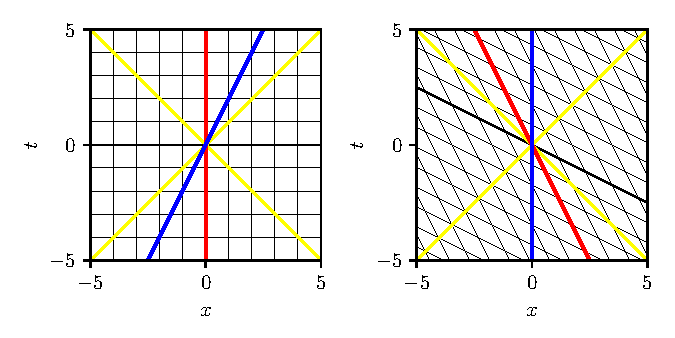
\includegraphics[width=3.2in, height = 1.6in]{images/k1.pdf}
			\caption{A Lorentz Transformation $(k=1)$}
			\label{fig:lorentzk1}
		\end{figure}

		\begin{figure}[h!]
			\centering
			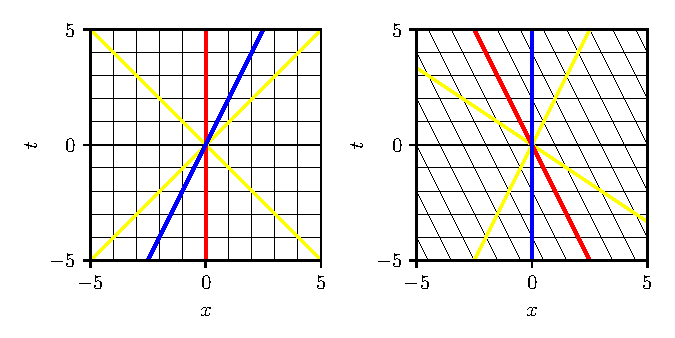
\includegraphics[width=3.2in, height = 1.6in]{images/k0.pdf}
			\caption{A Galilean Transformation $(k=0)$}
			\label{fig:lorentzk0}
		\end{figure}

		\begin{figure}[h!]
			\centering
			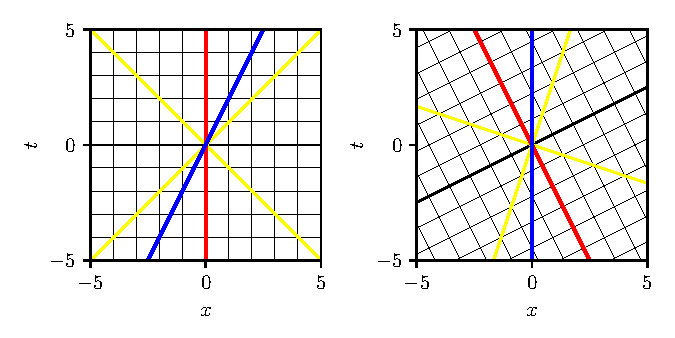
\includegraphics[width=3.2in, height = 1.6in]{images/k-1.pdf}
			\caption{A $k<0$ Lorentz Transformation $(k=-1)$}
			\label{fig:lorentzk-1}
		\end{figure}

	\end{solution_pset}
	\ 
	\newpage
	% ===========================
	% PROBLEM 1.2
	% ===========================
	\stepcounter{subsection}
	\subsection*{
		Problem 1.2
	}
	\begin{problem}
		To get the conditions above, we required closure--- i.e.,
		that the composition of two frame transformations $S\to S'$
		and $S'\to S''$ is also a frame transformation, $S\to S''$.
		You will notice that we only used equality of the diagonal 
		components of the composite transformation to get the equation
		in the problem above. What about the off diagonal components? Explore.
	\end{problem}
	\begin{solution_pset}
		We again refer to \S1.4\cite{juan2026}. For a velocity $w$ with respect from reference frame $S$ 
		to $S''$, transformation obtained has general form
		\begin{equation}
			\label{eq:Mw}
			M\indices{^\mu_\nu}(w)
			=
			\bmqty{
				A(w) & -vA(w) \\[4pt]
				- \dfrac{(A(w)^2-1)}{vA(v)} 
					 & A(w)
			}
		\end{equation}
		As we imposed from the closure condition, we also require
		that the composion of a transformation is also a transformation.
		For velocity $v$ with respect from $S$ to $S'$, and $u$, with respect to 
		$S'$ to $S''$, we have
		\begin{equation}
			\label{eq:Mw-MvMu}
			\tensor{M}{^\mu_\sigma}(w) = \tensor{M}{^\mu_\nu}(u)\tensor{M}{^\nu_\sigma}(v)
		\end{equation}
		Explicitly showing the multiplication, we have
		\[
			\tensor{M}{^\mu_\nu}(w) = 
			\bmqty{
				A(u) & -uA(u) \\[4pt]
				- \dfrac{(A(u)^2-1)}{uA(u)} 
					 & A(u)
			}
			\bmqty{
				A(v) & -vA(v) \\[4pt]
				- \dfrac{(A(v)^2-1)}{vA(v)} 
					 & A(v)
			}
		\]
		Solving that, we have the following monstrous matrix multiplication:
		{
			\begin{equation*}
			\tensor{M}{^\mu_\nu}(w) = 
			\begin{bmatrix}
				A(u)A(v) + \dfrac{uA(u)\bigl(A(v)^2-1\bigr)}{vA(v)} & 
				-(u+v)A(u)A(v) \\[14pt]
				-\dfrac{\bigl(A(u)^2-1\bigr)A(v)}{uA(u)} - \dfrac{A(u)\bigl(A(v)^2-1\bigr)}{vA(v)} & 
				A(u)A(v) + \dfrac{vA(v)\bigl(A(u)^2-1\bigr)}{uA(u)}
			\end{bmatrix}
			\end{equation*}
		}
		We used the equality of diagonal components, i.e, $M\indices{^0_0}$ and $M\indices{^1_1}$, 
		to derive (\ref{eq:A-value}). Now, we are tasked to determine the implications
		of the off-diagonal components, i.e., $M\indices{^0_1}$ and $M\indices{^1_0}$.

		The tricky part here is discerning what it means. The off-diagonal components are not equal, so 
		I can't put a relationship between them, so it took a long time for me to 
		think about what it means. However, I realized that we can again exploit closure.
		That is, components of $M(w)$ must be equal to components of $M(u) M(v)$.
		Also, we already know the value of $A(w)$, which is just (\ref{eq:A-value})
		\[
			A(w) = \frac{1}{\sqrt{1-kw^2}}
		\]
		As a preliminary, we begin with the established result on the lecture, that
		the $M\indices{^1_0}$ reduces to
		\begin{align*}
			-
		   \frac{A(w)^2 - 1}{w A(w)} 
		   &=
		   -
		   \frac{
			   \pqty{\frac{1}{\sqrt{1-kw^2}}}^2 - 1
		   }{w A(w)} \\
		   &=
		   -
		   \frac{
			   {\frac{1}{{1-kw^2}}} - 1
		   }{w A(w)} \\
		   &=
		   -
		   \frac{
			   {\frac{1 - (1-kw^2)}{{1-kw^2}}} 
		   }{w A(w)} \\
		   &=
		   -
		   \frac{
			   {\frac{kw^2)}{{1-kw^2}}} 
		   }{w A(w)} \\
		   &=
		   -
		   \frac{
			   kw^2 A(w)^2
		   }{w A(w)} \\
		   &=
		   -kw A(w)
		\end{align*}
		However, look at $M\indices{^1_0}$, it is just $-w A(w)$.
		Hence, we show the relation between these two components:
		\begin{equation}
			\label{eq:M01-M10 relation}
			M\indices{^0_1} 
			=
			k
			M\indices{^1_0} 
		\end{equation}
		
		With that establish, lets begin working on the problem.
		We start with $M\indices{^1_0}(w)$. By closure, we require that
		\begin{equation}
			\label{eq:M10-equality}
		    w A(w) = (u + v) A(u) A(v)
		\end{equation}
		Likewise, with $M\indices{^0_1}$, we require that
		\begin{equation}
			\label{eq:M01-equality}
			\dfrac{(A(w)^2-1)}{wA(w)} 
			=
			\dfrac{\bigl(A(u)^2-1\bigr)A(v)}{uA(u)} + \dfrac{A(u)\bigl(A(v)^2-1\bigr)}{vA(v)}  
		\end{equation}
		
		We can show that (\ref{eq:M01-equality}) just 
		reduces to (\ref{eq:M10-equality})
		\begin{align*}
			\dfrac{(A(w)^2-1)}{wA(w)} 
			&=
			\dfrac{\bigl(A(u)^2-1\bigr)A(v)}{uA(u)} 
			+
			\dfrac{A(u)\bigl(A(v)^2-1\bigr)}{vA(v)} \\
			\dfrac{kw^2A(w)^2}{wA(w)} 
			&=
			\dfrac{\bigl(ku^2 A(u)^2 \bigr)A(v)}{uA(u)} 
			+
			\dfrac{A(u)\bigl(kv^2 A(v^2)\bigr)}{vA(v)} \\
			kwA(w)
			&=
			kvA(u)A(v)
			+
			kvA(u)A(v)\\
			wA(w)
			&=
			(u+v)
			A(u) A(v)
		\end{align*}

		What we note here is that (\ref{eq:M10-equality}) 
		provides us a consistency condition which determines 
		how $A$ must compose. Now, if we use (\ref{eq:A-value}),
		we find that
		\[ 
			\frac{w}{\sqrt{1 - kw^2}} 
			=
			\frac{u+v}{
				\sqrt{1 - ku^2} 
				\sqrt{1 - kv^2} 
			} 
		\]
		We massage this a bit and look at what we find.
		Consider:
		\begin{align*}
			\frac{w^2}{{1 - kw^2}} 
			&=
			\frac{(u+v)^2}{
				{
					(1 - ku^2)
				} 
				{
					(1 - kv^2)
				} 
			} 
			\\
			w^2
			\pqty{1 - ku^2}
			\pqty{1 - kv^2}
			&=
			(u+v)^2 
			\pqty{1 - kw^2}\\
			w^2
			\pqty{1 - ku^2 - kv^2 + k^2 u^2 v^2}
			&=
			(u+v)^2 
			- kw^2(u+v^2)\\
			w^2
			\pqty{1 - ku^2 - kv^2 + k^2 u^2 v^2}
			+ 
			kw^2(u+v^2)
			&=
			(u+v)^2 \\
			w^2
			\pqty{
				1 - 
				ku^2 - 
				kv^2 + k^2 u^2 v^2 + 
				k(u+v)^2
			}
			&=
			(u+v)^2 \\
			w^2
			\pqty{
				1 - 
				ku^2 - 
				kv^2 + k^2 u^2 v^2 + 
				ku^2 + 2kuv + kv^2
			}
			&=
			(u+v)^2 \\
			w^2
			\pqty{
				1 +
				2kuv + 
				k^2 u^2 v^2 
			}
			&=
			(u+v)^2 \\
			w^2
			(1 + kuv)^2
			&=
			(u+v)^2 \\
			w^2
			&=
			\frac{
				(u+v)^2 
			}{
				(1 + kuv)^2
			} 
		\end{align*}
		Hence, from the equivalence of $M\indices{^1_0}(w) = 
		M\indices{^1_0}(u) 
		M\indices{^1_0}(v) 
		$,
		and the from the scaling factor
		of the components.
		$
		M\indices{^1_0}(w)
		=
		k 
		M\indices{^0_1}(w)
		$,
		out comes the relativistic velocity
		addition law.
		\begin{equation}
			\label{eq:w=u+v}
			\boxed{
				w
				=
				\frac{
					u+v
				}{
					1 + kuv
				}
			}
		\end{equation}

		Note that this relation can be independently
		derived simply from knowing the value of $A$,
		and taking the velocities to be 
		\[
			w = \dv{x}{t} 
		\]
		from $S$ to $S'$,
		and
		\[
			u = \dv{x'}{t'} 
		\]
		from $S''$ to $S'$. You can then do some math
		and still arive with the velocity addition formula.

		However, here we see that the notion velocity addition
		between two moving frames of reference
		is embedded in the components of the transformation itself.
		
	\end{solution_pset}
	\newpage
	% ===========================
	% PROBLEM 1.3
	% ===========================
	\stepcounter{subsection}
	\subsection*{
		Problem 1.3
	}
	\begin{problem}
		Given a basis for a vector space $V$, $\{\vec{e}_i\}, i = 1,\ldots,n$, we considered
		the set of $n$ dual vectors $\{\underline{e}^i\}$ according to the rule
		\begin{equation}
			\label{eq:1.3.1}
			\underline{e}^i[\vec{e}_j] = \tensor{\delta}{^i_j}
		\end{equation}
		\begin{enumerate}[(1)]
			\item Show that this rule is suffient to define the $\underline{e}^i$  as dual
				vectors. That is, we know how each $\underline{e}^i$ acts on all $v\in V$.
			\item Show that $\{\und{e}^i\}$ is a basis for $V^*$.
		\end{enumerate}
	\end{problem}
	\begin{solution_pset}
		% \begin{enumerate}(1)
		    % \item Suffiency of definining it as a dual vector:

				% \begin{proof}
				% \begin{align*}
					% \forall v \in V,\quad \qty{e_\mu} \subset V,\quad \Span{\{e_\mu\}} = V, \qty{e_\mu}&:\\
					% \implies v &= v^\mu e_\mu\\
					% e^\nu[v] &= e^\nu[v^\mu e_\mu]\\
					% e^\nu[v] &= v^\mu e^\nu[e_\mu]\\
					% e^\nu[v] &= v^\mu \delta\indices{^\nu_\mu} \\
					% e^\nu[v] &= v^\nu \\
					% \therefore e^\nu &\in V^*
				% \end{align*}
				% \end{proof}
					
			% \item LI \& spanning
				% \begin{enumerate}

				    % \item LI
						% \begin{proof}
						% \begin{align*}
							% \forall e^\mu \in V^*,\quad e_\nu \in V&\\
							% \forall a_\mu : a_\mu e^\mu &= \und{0}\\
							% \implies a_\mu e^\mu[e_\nu] &= 0\\
							% a_\mu \delta^\mu_\nu &= 0\\
							% \implies\forall a_\nu: a_\nu &= 0\\
							% \implies LI\{e^\mu\} 
						% \end{align*}
						% \end{proof}
						
					% \item Spanning
						% \begin{proof}
						% \begin{align*}
							% \exists e_\mu: e_\mu \in V,\quad& LI \{e_\mu\}, \Span{\{e_\mu\}}=V\\
							% \exists \omega \in V^*&:\\
							% \omega_\mu &= \omega[e_\mu]\\
							% \forall v\in V&:\\
							% \omega[v] &= \omega_\mu e^\mu[v]\\
							% \implies\omega &= \omega_\mu e^\mu\\
							% \therefore \Span{\{e^\mu\}} &= V^* 
						% \end{align*}
						% \end{proof}
				% \end{enumerate}
		% \end{enuerate}
		
		\textit{Note:} I use $\ovr{v}$ instead of $\vec{v}$, it's cleaner looking.

		\begin{enumerate}[(1)]
			\item Suffiency of definining $\und{e}^i$ as a dual vector.

				For the rule $\und{e}^i[\ovr{e}_j]=\delta\indices{^i_j}$ to define $\und{e}^i$ as a dual vector, 
				  we must know how 
				  each $\und{e}^i$ acts on $\ovr{v}$, $\forall \ovr{v}\in V$.

				  By definition (\S 2.6, \cite{juan2026}), a dual vector
				  is a linear map acting on a vector such that, if $\und\omega\in V^*$,
				  $\ovr v\in V$, then
				  \[
					  \omega: V\to \R,\quad \ovr v \mapsto\und\omega[\ovr v]\in \R
				  \]

					\begin{proof}
						Let $\ovr v\in V$. Since $\{\ovr{e}_\mu\}$ is a basis of $V$,
						there exist unique components $v^\mu\in\R$ such that
						\[
							\ovr{v}=v^\mu \ovr{e}_\mu.
						\]
						Then
						\begin{align*}
							\und{e}^\nu[\ovr v]
							&=\und{e}^\nu[v^\mu \ovr{e}_\mu]\\
							&=v^\mu \und{e}^\nu[\ovr{e}_\mu]\\
							&=v^\mu \delta^\nu_\mu\\
							&=v^\nu.
						\end{align*}
						Thus, the action of $\und{e}^\nu$ on every $\ovr v\in V$ is
						completely determined. 
					\end{proof}
			\item For $\qty{\und{e}^i}$ to be a basis, it must be both linearly independent and 
				  spans the entire dual vector space. We prove these two separately.
			
				\begin{enumerate}

					\item Linear Independence.

						If $\qty{\und{e}^i}$ is linearly independent, we note that
						$\forall a_\mu \in \R$, if
						\[
							a_\mu \und{e}^\mu =\und 0,
						\]
						then it implies that $\forall \mu, \mu \in (1,\ldots,n)$,
						\[
							a_\mu = 0.
						\]
						\begin{proof}
							Consider a linear combination such that
							\[
								a_\mu \und e^\mu = \und 0,
							\]
							where $a_\mu\in\mathbb{R}$ are arbitrary.

							Evaluating both sides on $e_\nu\in V$ gives
							\begin{align*}
								a_\mu \und e^\mu[\ovr e_\nu]
								&=\und 0[\ovr e_\nu]\\
								a_\mu\delta^\mu_\nu
								&=0\\
								a_\nu&=0.
							\end{align*}
							Since this holds for every $\nu$, we have
							$a_\mu=0$ for all $\mu$. Hence
							$\{\und e^\mu\}$ is linearly independent.
						\end{proof}
					\item Spanning

						For $\mathrm{span} \qty{\und e^i} = V^*$, it means that
						$\forall \und\omega\in V^*$, $\und\omega$ can be built as a linear combination of the basis vectors,
						i.e.,
						\[
							\und\omega = \omega_\mu \und e^\mu
						\]
						\begin{proof}
							Let $\omega\in V^*$. We define that
							\[
								\omega_\mu=\und \omega[\ovr e_\mu].
							\]
							For any $\ovr v\in V$, we can write
							\[
								\ovr v=v^\mu \ovr e_\mu.
							\]
							Then
							\begin{align*}
								\und\omega[\ovr v]
								&=\und\omega[v^\mu \ovr e_\mu]\\
								&=v^\mu\und\omega[\ovr e_\mu]\\
								&=v^\mu\omega_\mu \\
								&= \omega_\mu v^\mu\\
								&=\omega_\mu \und e^\mu[v].
							\end{align*}

							Since $v$ is arbitrary, we can remove it and
							retain the covector in an operational sense.
							Therefore,
							\[
								\und\omega=\omega_\mu \und e^\mu,
							\]
							so any $\und \omega\in V^*$ is a linear combination
							of $\und e^\mu$. Therefore
							\[
								\mathrm{span}{\{\und e^\mu\}}=V^*.
							\]
							That is, $\und e^\mu$ spans the covector space.
						\end{proof}
				\end{enumerate}

				Hence, $\und e^i$ is a basis for $V^*$.
		\end{enumerate}

	\end{solution_pset}
	\newpage
	% ===========================
	% PROBLEM 1.4
	% ===========================
	\stepcounter{subsection}
	\subsection*{
		Problem 1.4
	}
	\begin{problem}
		Show that if $\{\und{e}^i\}$ is a basis for $V^*$ and 
		$\{\vec{e}_i\}$ is a basis for $V$, then $\qty{\vec{e}_i\otimes \und{e}^j \otimes \und{e}^k}$, $i,j,k = 1,\ldots,n$, is 
		a basis for the space of $(1,2)$ tensors.
	\end{problem}
	\begin{solution_pset}
		
		To show that $\qty{\ovr e_i \otimes \und e^j \otimes \und e^k}$, where $i,j,k=1,\ldots, n$
		is a basis for (1,2) tensors, we must prove that
		it is linearly independent and spans the entire $(1,2)$ tensor space.
		We shall prove these separately.

		\textit{Note:} I will be using abstract index notation here. Also, I will be switching the indices on the basis vectors and covectors to greek because it makes the math easier.

		\begin{enumerate}[(1)]
		    \item Linear Independence.

				% Let the tensor set be 
				% \[
				% 	(T)\indices{^\alpha_{\beta\gamma}}
				% 	=
				% 		\qty{
				% 			\ovr e_\alpha
				% 			\otimes
				% 			\und e^\beta
				% 			\otimes
				% 			\und e^\gamma
				% 		}.
				% \]
				% Here, we denote that $T$ is a tensor for each choice of index $\alpha,\beta,\gamma = 1,\ldots, n$.
				% The parenthesis is there to specify that it is not a component, but rather, a set of tensors. Each choice
				% of index represents members of the basis as the indices $\alpha,\beta,\gamma$, or whatever is specified, varies.

				Let $0\indices{^{a}_{bc}}$ be the zero tensor for the
				$(1,2)$ tensor space, i.e., it maps all covector and vector
				arguments to $0$.

				The set of tensors $
				%	{(T)\indices{^{\alpha}_{\beta\gamma}}}
					\qty{
						\ovr e_\alpha \otimes \und e^\beta \otimes \und e^\gamma
					}
				$ is linearly independent
				if, for all $C\indices{_\alpha^{\beta\gamma}}\in\R$,
				\[
					C\indices{^\alpha_{\beta\gamma}}\ 
					\ovr e_\alpha \otimes \und e^\beta \otimes \und e^\gamma
					=
					0\indices{^{a}_{bc}}
				\]
				implies
				\[
					C\indices{^\alpha_{\beta\gamma}}=0
				\]
				for all $\alpha,\beta,\gamma=1,\ldots,n$.
				% \footnote{I am under the impression here 
				% that \textit{top} and \textit{bottom} index order does not matter, i.e., $C\indices{_\alpha^{\beta\gamma}} = C\indices{^{\beta\gamma}_\alpha}$}.

				\begin{proof}
					% Let
					% \[
					% 	T\indices{^{a}_{bc}}
					% 	=
					% 	{
					% 		\ovr e_\alpha
					% 		\otimes
					% 		\und e^\beta
					% 		\otimes
					% 		\und e^\gamma
					% 	}.
					% \]
					Consider $C\indices{^\alpha_{\beta\gamma}}\in\R$ such that
					\[
						C\indices{^\alpha_{\beta\gamma}}\ 
						% T\indices{^{a}_{bc}}
						\ovr e_\alpha \otimes \und e^\beta \otimes \und e^\gamma
						=
						0\indices{^{a}_{bc}}.
					\]
					Let's feed the tensor a set of basis covectors and vectors,
					$\und e^\lambda,\ovr e_\mu,\ovr e_\nu$.
					Then
					\begin{align*}
						C\indices{^\alpha_{\beta\gamma}}\ 
						% T\indices{^{a}_{bc}}
						\ovr e_\alpha \otimes \und e^\beta \otimes \und e^\gamma
						[
							\und e^\lambda,
							\ovr e_\mu,
							\ovr e_\nu
						]
						&=
						0\indices{^{a}_{bc}}
						[
							\und e^\lambda,
							\ovr e_\mu,
							\ovr e_\nu
						]
						\\
						% C\indices{_\alpha^{\beta\gamma}}
						% \ovr e_\alpha
						% \otimes
						% \und e^\beta
						% \otimes
						% \und e^\gamma
						% [
						% 	\und e^\lambda,
						% 	\ovr e_\mu,
						% 	\ovr e_\nu
						% ]
						% &=0
						% \\
						C\indices{^\alpha_{\beta\gamma}}\ 
						\ovr e_\alpha[\und e^\lambda]
						\und e^\beta[\ovr e_\mu]
						\und e^\gamma[\ovr e_\nu]
						&=0
						\\
						C\indices{^\alpha_{\beta\gamma}}
						\delta\indices{^\lambda_\alpha}
						\delta\indices{^\beta_\mu}
						\delta\indices{^\gamma_\nu}
						&=0
						\\
						C\indices{^\lambda_{\beta\gamma}}
						\delta\indices{^\beta_\mu}
						\delta\indices{^\gamma_\nu}
						&=0
						\\
						C\indices{^\lambda_{\mu\gamma}}
						\delta\indices{^\gamma_\nu}
						&=0
						\\
						C\indices{^\lambda_{\mu\nu}}
						&=0.
					\end{align*}
					Since the indices $\lambda,\mu,\nu$ are arbitrary, we can replace them. Hence,
					\[
						C\indices{^\alpha_{\beta\gamma}}=0
					\]
					for all $\alpha,\beta,\gamma$.
				\end{proof}
				
				
			\item Spanning

				A set of tensors $
					% \qty{T\indices{^{a}_{bc}}}
					\qty{
						\ovr e_\alpha \otimes \und e^\beta \otimes \und e^\gamma
					}
				$ span the tensor space $(1,2)$,
				if an arbitrary tensor $G\indices{^{a}_{bc}}$ can be written as a linear
				combination of the tensor set $G\indices{^\alpha_{\beta\gamma}}\in \R, \forall \alpha,\beta,\gamma = 1,\ldots,n$, i.e.,
				\[
					G\indices{^{a}_{bc}}
					 = 
					 G\indices{^{\alpha}_{\beta\gamma}}\ 
					\ovr e_\alpha \otimes \und e^\beta \otimes \und e^\gamma
				\]

				\begin{proof}
					% Let 
					% \[
					% 	T\indices{^a_{bc}} = \ovr e_\lambda \otimes \und e^\mu \otimes \und e^\nu
					% \]

					We define the following: 

					For an arbitrary tensor $G\indices{^a_{bc}}$,
					we define that the components are given by\footnote{
						I kinda feel like this move is a hack of some sort.
						Feels like a circular argument without really having justification.
						I don't understand why we define it to be like that (other 
						than to define it in terms of the basis itself), but the lecture defined things like
						this multiple times so yeah, just kinda followed it.
					}
					\[
						G\indices{^\alpha_{\beta\gamma}}
						\equiv
						G\indices{^a_{bc}} 
						[
							\und e^\alpha,
							\ovr e_\beta,
							\ovr e_\gamma
						]
					\]
					Thus, let's feed the basis covectors and vectors $
							\und e^\lambda,
							\ovr e_\mu,
							\ovr e_\nu
					$
					\begin{align*}
						G\indices{^a_{bc}} 
						[
							\und e^\lambda,
							\ovr e_\mu,
							\ovr e_\nu
						]
						&=
						G\indices{^\lambda_{\mu\nu}}
						\\
						&=
						G\indices{^\alpha_{\mu\nu}}
						\delta\indices{^\lambda_\alpha}
						\\
						&=
						G\indices{^\alpha_{\beta\nu}}
						\delta\indices{^\lambda_\alpha}
						\delta\indices{^\beta_\mu}
						\\
						&=
						G\indices{^\alpha_{\beta\gamma}}\ 
						\delta\indices{^\lambda_\alpha}
						\delta\indices{^\beta_\mu}
						\delta\indices{^\gamma_\nu}
						\\
						&=
						G\indices{^\alpha_{\beta\gamma}}\ 
						\ovr e_{\alpha}
						[\und e^\lambda]
						\und e^{\beta}
						[\ovr e_\mu]
						\und e^{\gamma}
						[\ovr e_\nu]
						\\
						&=
						G\indices{^\alpha_{\beta\gamma}}
						(
							\ovr e_\alpha \otimes 
							\und e^\beta \otimes 
							\und e^\gamma
						)
						[
							\und e^\lambda,
							\ovr e_\mu,
							\ovr e_\nu
						]
					\end{align*}
					However, the term in the parenthesis is just
					% $T\indices{^a_{bc}}$,
					the tensor set,
					thus
					\begin{align*}
						G\indices{^a_{bc}} 
						[
							\und e^\alpha,
							\ovr e_\beta,
							\ovr e_\gamma
						]
						&=
						G\indices{^\alpha_{\beta\gamma}}\ 
						\ovr e_\alpha \otimes \und e^\beta \otimes \und e^\gamma
						[
							\und e^\lambda,
							\ovr e_\mu,
							\ovr e_\nu
						]
					\end{align*}
					Since the arguments $
						\und e^\lambda,
						\ovr e_\mu,
						\ovr e_\nu
					$ are arbitrary, we can remove them and retain
					the tensor as an operator. Therefore
					\begin{align*}
						G\indices{^a_{bc}} 
						&=
						G\indices{^\alpha_{\beta\gamma}}\ 
						% T\indices{^a_{bc}}
						\ovr e_\alpha \otimes \und e^\beta \otimes \und e^\gamma
						\\
						\implies
						\mathrm{span}\qty{
							\ovr e_\alpha \otimes \und e^\beta \otimes \und e^\gamma
						}
						&=
						\binom{1}{2}
					\end{align*}
					% Since $\lambda, \mu,$ and $\nu$ are arbitrary,
					% we can replace them.
					% \begin{align*}
					% 	G\indices{^a_{bc}} 
					% 	&=
					% 	G\indices{^\alpha_{\beta\gamma}}
					% 	T\indices{^a_{bc}}\\[1em]
					% 	\implies
					% 	\mathrm{span}\qty{T\indices{^a_{bc}}} 
					% 	&=
					% 	\binom{1}{2}
					% \end{align*}
					Thus, the tensors
					\[
						\qty{
							\ovr e_\alpha \otimes \und e^\beta \otimes \und e^\gamma
						}
					\]
					span the $(1,2)$ tensor space.
				\end{proof}
		\end{enumerate}
		Hence, $
		\qty{\ovr e_\alpha \otimes \und e^\beta \otimes \und e^\gamma}
		$ constitute a basis for the $(1,2)$ tensor space.

	\end{solution_pset}
	\newpage
	% ===========================
	% PROBLEM 1.5
	% ===========================
	\stepcounter{subsection}
	\subsection*{
		Problem 1.5
	}
	\begin{problem}
		If $g$ is a $(0,2)$ tensor, then it defines an isomorphism between $V$ and $V^*$,
		i.e., $g:V\to V^*$. Show that the inverse map $g\inv: V^* \to V$, such that 
		$g\inv g = gg\inv = \mathrm{Id}$, is a $(2,0)$ tensor.
	\end{problem}
	\begin{solution_pset}
			\begin{proof}
				A $(2,0)$ tensor is a bilinear map such that, if $\alpha\in(2,0), \omega,\eta\in V^*$
				\[
					\alpha:V^*\times V^*\to \R,\qquad \alpha:\omega,\eta\mapsto \alpha(\omega,\eta).
				\]

				Now we figure out how to massage $g\inv$ to show this property.
				Since $g\in(0,2)$ it accepts two vectors and returns a scalar. 
				However, it can also only accept one,
				and can be defined as a map such that
				\[
					g: V \to V^*.
				\]
				We have the inverse map be 
				\[
					g\inv: V^* \to V.
				\]
				That is, it maps covectors to vectors. Let $\omega,\eta\in V^*$,
				then
				\[
					g\inv(\omega) \in V.
				\]
				Since $\eta$ is a covector, it's a map from $V\to \R$. Hence, we can
				have $\eta$ act on $g\inv(\omega)$,
				\[
					\eta(g\inv(\omega))\in\R.
				\]
				Let us define $g\inv$ to accept two arguments, such that
				\[
					g\inv(\omega,\eta)\equiv
					\eta(g\inv(\omega)) \in \R.
				\]
				Thus, we have shown that $g\inv$ can be a map such that
				\[
					g\inv:V^*\times V^* \to \R.
				\]
				However, this is not enough to include it in the group of $(2,0)$ tensors.

				Since $g\inv:V^* \to V$ is an isomorphism, it implies linearity between covectors, i.e.,
				\[
					g\inv(a \omega_1 + b \omega_2) = a g\inv(\omega_1)+ b g\inv(\omega_2).
				\]
				Let us check bilinearity for two covectors. 

				For $a,b\in\R$, then
				\begin{align*}
					g\inv(a\omega_1 + \omega_2, \eta)
					&=
					\eta\qty(g\inv(a\omega_1 + b\omega_2))\\
					&=
					\eta\qty(g\inv(a\omega_1) + g\inv(b\omega_2))\\
					&=
					a \eta g\inv(\omega_1) + b \eta g\inv(\omega_2)\\
					&=
					a g\inv(\omega_1,\eta) + b  g\inv(\omega_2,\eta).
				\end{align*}
				Similarly,
				\[
					g\inv(\omega,a\eta_1 + b\eta_2) = a g\inv(\omega,\eta_1) + b g\inv(\omega,\eta_2).
				\]
				Thus, $g\inv$ is a bilinear on $V^* \times V^*$, and therefore, a $(2,0)$ tensor.
			\end{proof}

			No longer part of the main proof, but a less rigorous but quicker argument is this:
			Since $g$ is defined to be
			\[
				g = g_{\mu\nu}\p_\mu \otimes \p_\nu.
			\]
			Then its inverse, such that
			\[
				gg\inv = g\inv g = \delta,
			\]
			takes the form
			\[
				g\inv = g^{\mu\nu} \dd{x^\mu}\otimes \dd{x^\nu},
			\]
			where
			\[
				g^{\mu\alpha}g_{\alpha\nu} = \delta\indices{^\mu_\nu}.
			\]
			Hence, $g\inv$ is a $(2,0)$ tensor with components $g^{\mu\nu}$.
	\end{solution_pset}
	\newpage
	% ===========================
	% PROBLEM 1.6
	% ===========================
	\stepcounter{subsection}
	\subsection*{
		Problem 1.6
	}
	\begin{problem}
		Starting from the definition of a tensor as a multilinear map, prove the 
		standard transformation law for $(k,l)$-tensor components under a change of coordinates.
	\end{problem}
	\begin{solution_pset}
		The standard Tensor component transformation law under change of 
		coordinates from $\{x^\sigma\}$ to $\{x'^{\mu}\}$ is \cite{juan2026, Liang2023}
		\begin{equation}
			\label{eq:tensor-transformation-law}
			{T'}\indices{^{{\mu_1}\ldots{\mu_k}}_{{\nu_1}\ldots{\nu_l}}}
			=
			\pdv{x'^{\mu_1}}{x^{\rho_1}} 
			\cdots
			\pdv{x'^{\mu_k}}{x^{\rho_k}} 
			\pdv{x^{\sigma_1}}{x'^{\nu_k}} 
			\cdots
			\pdv{x^{\sigma_l}}{x'^{\nu_l}} 
			\tensor{T}{^{{\rho_1}\ldots{\rho_k}}_{{\sigma_1}\ldots{\sigma_l}}}
		\end{equation}
		We derive it, from the definition alone, as follows:

		\begin{proof}
		The definition of a tensor, as stated from the lecture, is (\S 2.7 \cite{juan2026}):

		A tensor of $(k,l)$ type is a multilinear map 
		from the product of dual and vector spaces to real numbers,
		such that
		\begin{equation}
			\label{eq:tensor-defn}
			T:
			V^*_1 \times 
			V^*_2 \times 
			\cdots
			V^*_k \times
			V_1 \times
			V_2 \times
			\cdots
			V_l
			\to \R
		\end{equation}
		That is, it is a \textit{machine} which accepts covectors ($k$ slots), and vectors ($l$ slots),
		and returns a real number. Multilinearity here means that the tensor is linear in each slot separately.

		Vectors are tensors which accept one covector, and likewise covectors are tensors which accept one vector.
		Hence, we can use basis vectors and basis covectors as a basis for a tensor space. Let $\{x^\mu\}$ 
		be coordinate functions in a manifold $\mcal M$, and 
		$T\in(k,l), \omega_i \in V^*, v^i\in V$
		such that we can define vectors and covectors naturally:
		\[
			v = v^\mu \p_\mu, \qquad \omega = \omega_\mu \dd{x^\mu}
		\]
		Therefore, the basis vectors are $\p_\mu$, and the basis covectors are $\dd{x^\mu}$.

		We define that if we feed the tensor basis vectors and covectors, we recover its components.
		\begin{align*}
			T[\dd{x^{\mu_1}},\cdots,\dd{x^{\mu_k}};\p_{\nu_1},\cdots,\p_{\nu_l}]
			\equiv
			T\indices{^{\mu_1\cdots \mu_k}_{\nu_1\cdots\nu_l}}\ 
		\end{align*}
		We can then expand our way into $k+l$ identity $\delta^{\mu_k}_{\nu_l}$ operations,
		pulling out the basis for each index, separating them, discovering it's an outer product,
		and recovering the tensor as an operational
		definition (see the solution on Problem 1.4.2 which uses this method).

		With all that done,
		we find that a tensor $T\in(k,l)$ defined in a chart $\{x^\mu\}$ 
		has component form, which is the form that we need 
		to define the transformation in general.
		\begin{equation}
			\label{eq:tensor-component-form}
			T = 
			T\indices{^{\mu_1\cdots \mu_k}_{\nu_1\cdots\nu_l}}\ 
			\p_{\mu_1}\otimes \cdots \otimes \p_{\mu_k}
			\otimes
			\dd{x^{\nu_1}}\otimes \cdots \otimes \dd{x^{\nu_1}}
		\end{equation}
		Say we wish to change our coordinates from $\{x^\mu\}$ to $\{y^\sigma\}$.
		Recall how a vector components transform under a change of coordinates:
		\begin{equation}
			\label{eq:vector-transform}
			\pdv{}{y^\sigma} = \pdv{x^\mu}{y^\sigma} \pdv{}{x^\mu} 
		\end{equation}
		Additionally, recall how a covector components transform under a change 
		of coordinates
		\begin{equation}
			\label{eq:covector-transform}
			\dd{y^\sigma} = \pdv{y^\sigma}{x^\mu}\dd{x^\mu} 
		\end{equation}
		Let's rewrite the expression it terms of this change of coordinates.
		We will now explicity write $\p_\mu = \pdv{}{x^\mu}$, since there 
		are multiple coordinates involved.

		We're going from $x^\mu$ to $y^\sigma$, so it's gonna be the 
		inverse of the expressions above.
		\[
			T 
			=
			T\indices{^{\mu_1\cdots \mu_k}_{\nu_1\cdots\nu_l}}\ 
			\pqty{
				\pdv{
					y^{\rho_1}
				}{
					x^{\mu_1}
				}
				\pdv{}{
					y^{\rho_1}
				} 
			}
			\otimes
			\cdots
			\otimes
			\pqty{
				\pdv{
					y^{\rho_k}
				}{
					x^{\mu_k}
				}
				\pdv{}{
					y^{\rho_k}
				} 
			}
			\otimes
			\pqty{
				\pdv{x^{\nu_1}}{y^{\sigma_1}}
				\dd{y^{\sigma_1}} 
			}
			\otimes
			\pqty{
				\pdv{x^{\nu_l}}{y^{\sigma_l}}
				\dd{y^{\sigma_l}} 
			}
		\]
			We can pull out the coordinate transformation coefficients, a.k.a. the Jacobians,
			they're just constants, and the tensor product is a linear operation.
			\begin{equation}
				\label{eq:transform-jacobians}
				T 
				=
					\pdv{
						y^{\rho_1}
					}{
						x^{\mu_1}
					}
					\cdots
					\pdv{
						y^{\rho_k}
					}{
						x^{\mu_k}
					}
					\pdv{x^{\nu_1}}{y^{\sigma_1}}
					\cdots
					\pdv{x^{\nu_l}}{y^{\sigma_l}}
				T\indices{^{\mu_1\cdots \mu_k}_{\nu_1\cdots\nu_l}}\ 
					\pdv{}{y^{\rho_1}} 
				\otimes
				\cdots
				\otimes
					\pdv{}{y^{\rho_k}} 
				\otimes
					\dd{y^{\sigma_1}} 
				\otimes
				\cdots
				\otimes
					\dd{y^{\sigma_l}} 
			\end{equation}
		On the other hand, since $T$ is the same tensor regardless
		of the coordinate system, we can write it in the terms of the $\{y^\sigma\}$
		coordinates directly. We denote the components for this new coordinates to be 
		$T'$
		\begin{equation}
			\label{eq:tensor-component-form-y}
			T = 
			{T'}\indices{^{\rho_1 \cdots \rho_k}_{\sigma_1\cdots\sigma_l}}\ 
			\pdv{}{y^{\rho_1}} \otimes \cdots \otimes \pdv{}{y^{\rho_k}} 
			\otimes
			\dd{y^{\sigma_1}}\otimes \cdots \otimes \dd{y^{\sigma_1}}
		\end{equation}
		Let's compare (\ref{eq:transform-jacobians}) and (\ref{eq:tensor-component-form-y}).
		They are equal, they have the same basis tensors. However, their components are not the same.
		But since both statements are equal, then the components of both forms must also
		be equal, only transformations from one another. Hence, we equate them, and find the following result:
		\begin{equation}
			\label{eq:tensor-component-transform}
			\boxed{
				{T'}\indices{^{\rho_1 \cdots \rho_k}_{\sigma_1\cdots\sigma_l}} 
				=
				\pdv{
					y^{\rho_1}
				}{
					x^{\mu_1}
				}
				\cdots
				\pdv{
					y^{\rho_k}
				}{
					x^{\mu_k}
				}
				\pdv{x^{\nu_1}}{y^{\sigma_1}}
				\cdots
				\pdv{x^{\nu_l}}{y^{\sigma_l}}
				T\indices{^{{\mu_1}\cdots{\mu_k}}_{{\nu_1}\cdots{\nu_l}}} 
			}
		\end{equation}

		Therefore, we have recovered (\ref{eq:tensor-transformation-law}),\footnote{
			With some caveats, it used $x'$ instead of $y$, which isn't really
			a problem since we can just relabel it, and the indices are 
			swapped, but indices are arbitrary, and the swapping is consistent.
			We can just rename it and swap them, but I am too tired, and I neither
			have the drive nor inclination to do so.
			It is equivalent to Eq. (\ref{eq:tensor-transformation-law}). Trust me bro.
		} which is how a component of a $(k,l)$ tensor transforms under a
		coordinate transformation.
		\end{proof}
		


	\end{solution_pset}
	% ===========================
	% PROBLEM 1.7
	% ===========================
	\stepcounter{subsection}
	\subsection*{
		Problem 1.7
	}
	\begin{problem}
		Show that the identity maps
		\begin{equation}
			\label{eq:Id1}
		    \Id_1 : V\to V,\ \Id_1(v)= v, \forall v\in V
		\end{equation}
		\begin{equation}
			\label{eq:Id2}
			\Id_2 : V*\to V*,\ \Id_2(\omega)= \omega, \forall v\in V^*
		\end{equation}
		Can be interpreted as the same $(1,1)$ tensor. What are its components?
		What does this tensor do when it is fed a one-form and a vector? 
		Does this remind you of any other tensorial operation?
	\end{problem}
	\begin{solution_pset}
			We tackle this one first with a functional approach,
			then we do the quicker coordinate-based route.
		\begin{proof}

			A $(1,1)$ identity tensor can be viewed as a map
			\[
				\binom{1}{1}:
				V\to V,\qquad 
				\binom{1}{1}:
				V^* \to V^*
			\]
			or equivalently, as a bilinear map
			\[
				\binom{1}{1}:
				V^*\times V\to \R
			\]

			We start with $\Id_1:V\to V$. 
			For any $v\in V$, then
			\[
				\Id_1[v]= v.
			\]
			We can turn this into a scalar-valued operation
			by feeding the resulting vector to a one-form $\omega\in V^*$:
			\[
				\omega[\Id_1[v]] = \omega[v]
			\]
			As we did in Problem 1.5, we can define this as a bilinear map, a $(1,1)$ tensor
			call it $\delta$\footnote{wow, what a shocker choice of name}, such that
			\[
				\delta(\omega,v) \equiv \omega[v]
			\]

			For $\Id_2:V^*\to V^*$, given $\omega\in V^*$,
			then
			\[
				\Id_2(\omega)= \omega
			\]
			A vector $v$ naturally acts on a one-form by evaluation.
			Alternatively, we could use the fact that the double-dual
			space $V^{**}$ is isomorphic to $V$, $V^{**}\cong V$, so 
			\[
				\Id_2(\omega)[v] \equiv v[\Id_2(\omega)] = \omega(v)
			\]
			Again, we find that
			\[
				\delta(\omega,v)= \omega[v]
			\]
			Both identity maps map $v$ and $\omega$ to the same 
			scalar value. Hence, it is the same $(1,1)$ tensor.
		\end{proof}

		Alternatively, since it a vector and a covector can be represented
		with a vector and covector basis,
		\[
			v = v^\mu \ovr e_\mu,\qquad  \omega = \omega_\nu \und e^\nu
		\]
		Then we have
		\begin{align*}
			\delta(\omega,v) 
			&= 
			\delta[
				v^\mu \ovr e_\mu,
				\omega_\nu \und e^\nu
			]\\
			&=
			v^\mu \omega_\nu \delta[\ovr e_\mu, \und e^\nu]\\
			&=
			v^\mu \omega_\nu \delta\indices{^\mu_\nu}\\
			&=
			v^\mu \omega_\nu
		\end{align*}
		That is, it is just the Euclidean tensor/metric,
		or the Kronecker delta, or whatever other name it has.

		Thus, its components are 
		\[
			\delta\indices{^\mu_\nu} = 
			\begin{cases}
			    1,\quad\mu=\nu\\
				0,\quad\mu\neq\nu
			\end{cases}
		\]
		Since it is a $(1,1)$ tensor, and matrices are isomorphic to $(1,1)$ tensors,
		it can be represented as a matrix
		\[
			\delta\indices{^\mu_\nu}
			=
			\bmqty{
				1 & 0 \\
				0 & 1
			} 
		\]
		When fed a one-form and a vector, it simply evaluates the
		one-form on the vector
		\[
			\delta(\omega,v) = \omega(v)
		\]

		Otherwise known as a contraction operation, where
		we contract the indices upstairs and downstairs.
		\[
			\delta\indices{^\mu_\nu} \omega_\mu v^\nu = \omega_\nu v^\nu = \omega(v)
		\]
		So the identity $(1,1)$ tensor is just the Euclidean metric, or 
		the Kronecker delta, or the identity under contraction operator.
		Among other names.
	\end{solution_pset}

\newpage

\newpage
	\renewcommand{\refname}{Additional References}
	\addcontentsline{toc}{subsection}{Additional References}
	\bibliographystyle{unsrturl}
	\bibliography{references}	
	\newpage
\section*{ \textit{Author's Note} }
	\addcontentsline{toc}{subsection}{Author's Note}
	\textit{A grandiose essay}
	\vspace{0.5cm}

	My journey in learning relativity is quite curious. When I was a child, I remember 
	wondering why things go down the way they do.
	My folks and those who are older would simply answer: That's just the way things are, it's gravity. \textit{Basta}. 
	Later on, when I was a little older, I picked up this old book called \textit{Science in Daily Life} where I learned
	much about science and chemistry and all those good shit. That book was one of my prized possessions,
	I still have it today, in fact. When I was a little older, right around fourth grade, my neighbor
	was throwing out books she no longer used, and part of that mixture were books on chemistry and 
	books on Physics for fourth year high school. 

	It was there where I learned about Newton and his apple. It was there where I learned about Einstein and
	binding energies and logic gates, of nuclear physics and atom bombs; where I learned that gravity is a force that drew upon it other 
	masses by the product of their quantities the inverse of the square of their distances. That made me interested in orbital mechanics,
	astronomy, the Apollo program. That book was one of the reasons why I am where I am today, the same way
	Vsauce and Veritasium inspired me when I was watching their videos when I was young. I say 
	all this, because we all have an origin story of some sort. Some story we call ours, that tells 
	our own humble beginnings. This was a story of how I fell in love with Physics, and why I chose it
	to be my career once I reached adulthood. That's why I decided to be a Physicist.

	Newton had origin stories. Einstein had an origin story. We must treasure where we came from, and 
	what it took for us to get there, is all I'm trying to say. Anyways, I first learned about general 
	relativity all those years ago, but thought it was very difficult and a hassle to understand. Understanding
	special relativity and its implications were much easier, but boy, GR is a whole 'nother level. 
	But fascinating! Differential geometry, manifolds, paradoxes, black holes, all so fascinating and interesting
	for me, part of the reason why I fell in love with the damn philosophy of reason. But also, it was scary,
	all those numbers and derivatives and the like, all so intimidating, that I thought back then I 
	would never even learn it. And so, I 
	find it funny, now, as an adult, that I took it as my undergraduate specialty of choice, joining
	a laboratory that specialized in gravity, taking my thesis on gravity. The amount of difficult mathematics
	one had to master to reach this point is insane, but, much like a mountain, the difficulty is part
	of the journey, and to reach the top is sweeter than the pleasures we get to enjoy in our daily life.

	And so, here I am today, taking a graduate course in my undergraduate degree, about the subject that
	fascinated me as a child, but I found too difficult to climb and learn. Now, I know enough to say
	that what I know is a drop in an endless ocean, and relativity, the jewel of modern physics, in 
	both beauty and elegance, is the pearl at the bottom of it.
	It makes me glad that it is what I chose to dedicate my academic life to, and I find within me
	the desire to add to the sum of human knowledge, to participate in the accumulated species-wide project
	of humanity towards understanding nature, to leave a legacy behind and be remembered
	in such a way. It is only recently that I learned
	to appreciate physics for what it is, a beautiful description of reality. In my early college years, the
	stress of it all consumed me, so much so that I haven't really taken a break and looked at the landscape,
	and now I am about to graduate, I look back think of all those things 
	I learned, and it impresses me that I could learn so much.

	Anyways, these lecture notes are precisely that, transcriptions of lectures on the course of General Relativity,
	by one of the leading physicists in the country, Dr. Vega, whom I personally idolized since I
	learned about him when I was in highschool, being a homegrown gravitational physicist and all that,
	and now I'm studying under him as my adviser, ain't that something.
	The content is precisely what he talks about in the lecture. Although not exactly verbatim, I tried 
	my best to record all the words being said and tried to capture the topic being discussed at the moment,
	doing my best to convey all the ideas and meaning of the lecture. So that, in the future, I may look upon it when I forget something or simply
	as I please, and others, peers, students, friends, which I may give these lecture
	notes to, may understand it in a manner as I understand it today. I wish the future may be kind to us,
	and when we look back, to our stories and origins, may we smile and reminisce in mild happiness,
	and be proud of what we have become.

	\vfill
	\begin{flushright}
		{\Large
			\textbf{End.}
		}	
	\end{flushright}
	\begin{center}
		{
			\large
			\textsc{Physica Vincit Omnia}
		}
	\end{center}
\newpage
\addcontentsline{toc}{subsection}{Colophon}
	\thispagestyle{empty}
	\begin{center}
		\textit{Fideli meo computatro Lenovo 81AH, comite laboris, confectum}\\[0.5em]
		\textit{Typis \LaTeXe confectum}\\[1em]
		Augusto MMXXVI
	\end{center}
	\vspace*{1in}
	\begin{center}
		{\LARGE
			\textit{\textbf{
				Not\ae\ Lectionum\\
				de Relativitate Generali
			}}\\[2em]
		}
			\textit{Ex Lectionibus M. F. I. Vegae}\\[1em]
			\textit{Scriptae ab\\[0.5em] {\large\textbf{Argenteo Ioanne}}}\\[2in]
	\end{center}
	\vfill
	\begin{center}
		\textbf{IV – Baccalaureus Physic\ae}\\[0.5em]
		\textsc{Gravity Subgroup, GANAP Laboratory}\\[0.5em]
		{\large \textsc{National Institute of Physics}}\\
		{\large \textsc{University of the Philippines Diliman}}
	\end{center}
\newpage
	\thispagestyle{empty}
	\vspace*{0.5in}
	\begin{center}
		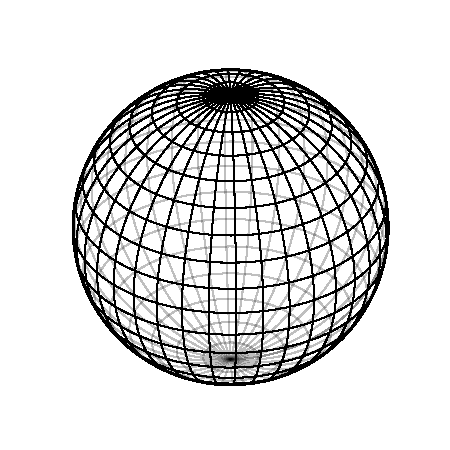
\includegraphics[width = 4in]{images/sphere.pdf}
	\end{center}
	\vfill
	\begin{center}
		{
			\Large
			\textsc{Sic Mundus Creatus Est}
		}
	\end{center}
\newpage
	\thispagestyle{empty}
	\begin{center}
		{
			\Large
			\textit{Ad Astra per Aspera}\\[2.5in]
			\textit{Hic sum, hic maneo}
			\vfill
			\textit{\textbf{Mors vincit Omnia}}
		}
	\end{center}

\end{document}
